\documentclass[12pt, a4paper, reqno, oneside]{book}
\usepackage[left=2.5cm, right=2cm, top=2cm, bottom=2cm]{geometry}
\usepackage{amsmath,amsxtra,amssymb,latexsym, amscd,amsthm}
\usepackage{microtype}
\usepackage{indentfirst}
\usepackage{color}
\usepackage{empheq}
\usepackage{iftex}
\ifXeTeX
  \usepackage{fontspec}
  \setmainfont[Ligatures=TeX]{Times New Roman}
  \setsansfont[Ligatures=TeX]{Arial}
  \usepackage[vietnamese,english]{babel}
\else
  \usepackage[utf8]{inputenc}
  \usepackage[T5]{fontenc}
  \usepackage[vietnamese]{babel}
\fi
% \usepackage{amsmath} % đã được nạp ở dòng 3
\usepackage[mathscr]{eucal}
\usepackage{amsfonts}
\usepackage{graphicx}
\usepackage{float}
\usepackage{listings}
\usepackage[dvipsnames]{xcolor}
\usepackage{verbatim}
\usepackage{tikz}
\usetikzlibrary{calc,positioning,arrows.meta,shapes.geometric,fit,backgrounds,decorations.pathreplacing}
\usepackage{tkz-graph}
\usepackage{array}
\usepackage{multirow}
\usepackage{algorithm}
\usepackage{algpseudocode}
% Note: subfigure is legacy and conflicts with modern subcaption; kept commented for compatibility
% \usepackage{subfigure}
\usepackage{pgfplots}
\pgfplotsset{compat=1.18}
\usepackage{titlesec}
\usepackage{fancyhdr}
\usepackage{rotating}
\usepackage{longtable}
\usepackage{supertabular}
\usepackage{subcaption}
\usepackage{tabularx}
\usepackage[normalem]{ulem}
\usepackage{pdfpages}
\usepackage[square,numbers]{natbib}
\usepackage{booktabs}
\usepackage{chngcntr}
\usepackage{tabularray}
\usepackage{placeins}
\usepackage{enumitem}
\usepackage{seqsplit}
\usepackage{needspace}
\usepackage[labelfont=bf, textfont=it, justification=centering]{caption}
\captionsetup{labelfont={color=blue, bf}, textfont=it}
\captionsetup[table]{position=top}
\captionsetup[figure]{position=bottom}

\hyphenation{op-tical net-works semi-conduc-tor}
\usepackage[hyphens,spaces,obeyspaces]{url}
\usepackage{xurl}
\usepackage[colorlinks=true,bookmarksopen,bookmarksnumbered,citecolor=blue,linkcolor=blue,urlcolor=blue,pdftitle={Biểu diễn cấu trúc cho hệ thống phát hiện xâm nhập mạng CAN bus đa phương tiện},pdfauthor={Vũ Tiến Tuấn Trung}]{hyperref}
\def\UrlBreaks{\do\/\do-\do_\do.\do=\do?\do&\do~}
\def\UrlNoBreaks{\do\(\do\[\do\{\do\<\do\:}
\setlength{\emergencystretch}{1.5em}

\renewcommand{\baselinestretch}{1.25}
\setlength{\headheight}{15pt}
\setlength{\textfloatsep}{10pt plus 2pt minus 2pt}
\setlength{\intextsep}{8pt plus 2pt minus 2pt}
\setlength{\floatsep}{8pt plus 2pt minus 2pt}
\setlength{\abovecaptionskip}{4pt}
\setlength{\belowcaptionskip}{4pt}
\titleformat{\section}{\normalfont\Large\bfseries\raggedright}{\thesection}{1em}{}
\titleformat{\subsection}{\normalfont\large\bfseries\raggedright}{\thesubsection}{1em}{}
\titleformat{\subsubsection}{\normalfont\normalsize\bfseries\raggedright}{\thesubsubsection}{1em}{}

\fancyhf{}
\fancyhead[L]{\small{\leftmark}}
\fancyfoot[C]{\thepage}

\newcommand\chap[1]{%
  \clearpage\phantomsection%
  \chapter*{#1}%
  \addcontentsline{toc}{chapter}{#1}%
  \markboth{#1}{}%
}
\newcommand\sect[1]{%
  \Needspace{5\baselineskip}%
  \phantomsection%
  \addcontentsline{toc}{section}{#1}%
  \section*{#1}%
}

\renewcommand{\theequation}{\thechapter.\arabic{equation}}
\counterwithin{algorithm}{chapter}
\renewcommand{\thealgorithm}{\thechapter.\arabic{algorithm}}
\floatname{algorithm}{Thuật toán}
\renewcommand{\listalgorithmname}{Danh sách thuật toán}
\algrenewcommand\algorithmicrequire{\textbf{Đầu vào:}}
\algrenewcommand\algorithmicensure{\textbf{Đầu ra:}}
\newtheorem{lemma}{\bf Bổ đề}[chapter]
\newtheorem{theorem}{\bf Định lý}[chapter]
\newtheorem{proposition}{\bf Mệnh đề}[chapter]
\newtheorem{corollary}{\bf Hệ quả}[chapter]
\newtheorem{definition}{\bf Định nghĩa}[chapter]
\newtheorem{remark}{\bf Chú ý}[section]

% Mức tiêu đề sâu (subsubsubsection, paragraph)
\titleclass{\subsubsubsection}{straight}[\subsection]
\newcounter{subsubsubsection}[subsubsection]
\renewcommand\thesubsubsubsection{\thesubsubsection.\arabic{subsubsubsection}}
\renewcommand\theparagraph{\thesubsubsubsection.\arabic{paragraph}}

\titleformat{\subsubsubsection}
  {\normalfont\normalsize\bfseries}{\thesubsubsubsection}{1em}{}
\titlespacing*{\subsubsubsection}
  {0pt}{3.25ex plus 1ex minus .2ex}{1.5ex plus .2ex}

\makeatletter
\renewcommand\paragraph{\@startsection{paragraph}{5}{\z@}%
  {3.25ex \@plus1ex \@minus.2ex}%
  {-1em}%
  {\normalfont\normalsize\bfseries}}
\renewcommand\subparagraph{\@startsection{subparagraph}{6}{\parindent}%
  {3.25ex \@plus1ex \@minus .2ex}%
  {-1em}%
  {\normalfont\normalsize\bfseries}}
\def\toclevel@subsubsubsection{4}
\def\toclevel@paragraph{5}
\def\toclevel@paragraph{6}
\def\l@subsubsubsection{\@dottedtocline{4}{7em}{4em}}
\def\l@paragraph{\@dottedtocline{5}{10em}{5em}}
\def\l@subparagraph{\@dottedtocline{6}{14em}{6em}}
\makeatother

\setcounter{secnumdepth}{4}
\setcounter{tocdepth}{2}

% Thư mục hình ảnh
\graphicspath{{./figs/}}

\definecolor{mygreen}{rgb}{0,0.6,0}
\definecolor{mygray}{rgb}{0.5,0.5,0.5}
\definecolor{mymauve}{rgb}{0.58,0,0.82}

\lstdefinestyle{customc}{
  belowcaptionskip=1\baselineskip,
  breaklines=true,
  frame=single,
  xleftmargin=\parindent,
  language=C,
  showstringspaces=false,
  basicstyle=\footnotesize\ttfamily,
  keywordstyle=\bfseries\color{green!40!black},
  commentstyle=\itshape\color{purple!40!black},
  identifierstyle=\color{blue},
  stringstyle=\color{orange},
  numbers=left,
  numberstyle=\tiny\color{gray},
  stepnumber=1, 
}

\lstdefinestyle{customasm}{
  belowcaptionskip=1\baselineskip,
  frame=single,
  xleftmargin=\parindent,
  language=[x86masm]Assembler,
  basicstyle=\footnotesize\ttfamily,
  commentstyle=\itshape\color{purple!40!black},
  numbers=left,
  numberstyle=\tiny\color{gray},
  stepnumber=1, 
}

\lstset{escapechar=@,style=customc}

\definecolor{processblue}{cmyk}{0.96,0,0,0}
\newcolumntype{C}[1]{>{\centering\arraybackslash}p{#1}}
\definecolor{eclipseStrings}{RGB}{42,0.0,255}
\definecolor{eclipseKeywords}{RGB}{127,0,85}
\colorlet{numb}{magenta!60!black}

\lstdefinelanguage{json}{
    basicstyle=\normalfont\ttfamily,
    commentstyle=\color{eclipseStrings},
    stringstyle=\color{eclipseKeywords},
    numbers=left,
    numberstyle=\scriptsize,
    stepnumber=1,
    numbersep=8pt,
    showstringspaces=false,
    breaklines=true,
    frame=lines,
    string=[s]{"}{"},
    comment=[l]{:\ "},
    morecomment=[l]{:"},
    literate=
        *{0}{{{\color{numb}0}}}{1}
         {1}{{{\color{numb}1}}}{1}
         {2}{{{\color{numb}2}}}{1}
         {3}{{{\color{numb}3}}}{1}
         {4}{{{\color{numb}4}}}{1}
         {5}{{{\color{numb}5}}}{1}
         {6}{{{\color{numb}6}}}{1}
         {7}{{{\color{numb}7}}}{1}
         {8}{{{\color{numb}8}}}{1}
         {9}{{{\color{numb}9}}}{1}
}

\DeclareRobustCommand{\code}[1]{\nolinkurl{#1}}
\newcolumntype{Y}{>{\raggedright\arraybackslash}X}
\newcolumntype{P}[1]{>{\raggedright\arraybackslash}p{#1}}

\begin{document}
\hypersetup{pageanchor=false}
\selectlanguage{vietnamese}

% =========================================================================
% TRANG BÌA NGOÀI (BÌA CHÍNH - KHUNG ĐÔI TIKZ)
% =========================================================================
\begin{titlepage}
\begin{center}
	\begin{tikzpicture}[overlay,remember picture]
	    \draw [line width=3pt,rounded corners=0pt]
	        ($ (current page.north west) + (20mm,-20mm) $)
	        rectangle
	        ($ (current page.south east) + (-15mm,20mm) $);
	    \draw [line width=1pt,rounded corners=0pt]
	        ($ (current page.north west) + (21.5mm,-21.5mm) $)
	        rectangle
	        ($ (current page.south east) + (-16.5mm,21.5mm) $);
	\end{tikzpicture}
	\\[1mm]
    \centerline{\bf ĐẠI HỌC QUỐC GIA HÀ NỘI}
    \centerline{\bf TRƯỜNG ĐẠI HỌC CÔNG NGHỆ}
    
    \vspace*{1.8cm}
    \large
        \begin{figure}[H]
        \centering
        
\includegraphics[width=0.23\linewidth]{figs/uet.jpg}
        \end{figure}
    \vspace*{1cm}
    \centerline{\bf VŨ TIẾN TUẤN TRUNG}
    \vspace*{2.0cm}
    {\fontsize{15}{19}\selectfont\bfseries
    \centerline{BIỂU DIỄN CẤU TRÚC CHO HỆ THỐNG}
    \centerline{PHÁT HIỆN XÂM NHẬP MẠNG CAN BUS}
    \centerline{ĐA PHƯƠNG TIỆN\par}}
    \vspace*{2.2cm}
    \centerline{\bf KHÓA LUẬN TỐT NGHIỆP ĐẠI HỌC HỆ CHÍNH QUY}
    \vspace*{0.2cm}
    \centerline{\bf Ngành: Hệ thống thông tin}
    
    \vfill
    \centerline{\bf Hà Nội -- 2026}
    \vspace{13pt}
\end{center}
\end{titlepage}

\newpage

% =========================================================================
% TRANG BÌA PHỤ (BÌA TRONG - CÓ CÁN BỘ HƯỚNG DẪN)
% =========================================================================
\begin{titlepage}
\begin{center}
	\begin{tikzpicture}[overlay,remember picture]
	    \draw [line width=3pt,rounded corners=0pt]
	        ($ (current page.north west) + (20mm,-20mm) $)
	        rectangle
	        ($ (current page.south east) + (-15mm,20mm) $);
	    \draw [line width=1pt,rounded corners=0pt]
	        ($ (current page.north west) + (21.5mm,-21.5mm) $)
	        rectangle
	        ($ (current page.south east) + (-16.5mm,21.5mm) $);
	\end{tikzpicture}
	\\[1mm]
    \centerline{\bf ĐẠI HỌC QUỐC GIA HÀ NỘI}
    \centerline{\bf TRƯỜNG ĐẠI HỌC CÔNG NGHỆ}
    \vspace*{1.8cm}
    \large
        \begin{figure}[H]
        \centering
        
\includegraphics[width=0.23\linewidth]{figs/uet.jpg}
        \end{figure}
    \vspace*{0.9cm}
    \large
    \centerline{\bf VŨ TIẾN TUẤN TRUNG}
    \vspace*{1.8cm}
    {\fontsize{15}{19}\selectfont\bfseries
    \centerline{BIỂU DIỄN CẤU TRÚC CHO HỆ THỐNG}
    \centerline{PHÁT HIỆN XÂM NHẬP MẠNG CAN BUS}
    \centerline{ĐA PHƯƠNG TIỆN\par}}
    \vspace*{1.5cm}
    \centerline{\bf KHÓA LUẬN TỐT NGHIỆP ĐẠI HỌC HỆ CHÍNH QUY}
    \vspace*{0.2cm}
    \centerline{\bf Ngành: Hệ thống thông tin}
    
    \vspace*{1.4cm}
    \centerline{\bf Cán bộ hướng dẫn:}
    \centerline{\bf PGS. TS. Nguyễn Ngọc Hóa}
    
    \vfill
    \centerline{\bf Hà Nội -- 2026}
    \vspace{13pt}
\end{center}
\end{titlepage}

\newpage
\hypersetup{pageanchor=true}
\pagenumbering{roman}
\pagestyle{plain}

% =========================================================================
% LỜI CẢM ƠN
% =========================================================================
\chap{Lời cảm ơn}
\vspace{20pt}
Em xin bày tỏ lòng biết ơn sâu sắc tới thầy hướng dẫn, PGS. TS. Nguyễn Ngọc Hóa, vì sự tận tâm dìu dắt, những góp ý chuyên môn quý báu và sự động viên liên tục trong suốt quá trình nghiên cứu và thực hiện khóa luận. Kiến thức uyên bác, sự phản biện chặt chẽ và định hướng khoa học của thầy đã giúp em vượt qua nhiều thách thức phương pháp luận để hoàn thành công trình này.

Em cũng xin chân thành cảm ơn các nhóm tác giả và cộng đồng nghiên cứu an ninh mạng ô tô đã công bố công khai các bộ dữ liệu đối chuẩn và công trình khoa học về mạng CAN, tạo điều kiện thiết yếu cho quá trình đối chứng và kiểm chứng thực nghiệm của khóa luận.

Trong quá trình thực hiện, tác giả có sử dụng các công cụ hỗ trợ AI cho việc rà soát ngữ pháp, định dạng văn bản, đối chiếu tài liệu và gợi ý cú pháp lập trình. Tác giả đã trực tiếp kiểm tra mọi nguồn trích dẫn, thẩm định và xác nhận toàn bộ mã nguồn, tự tiến hành thực nghiệm và hoàn toàn chịu trách nhiệm đối với nội dung khoa học cuối cùng; mọi ý tưởng cốt lõi, thiết kế phương pháp, phân tích và kết luận trong khóa luận đều là công trình nghiên cứu độc lập của tác giả.

Dù đã nỗ lực tối đa để bảo đảm tính chặt chẽ học thuật, khóa luận khó tránh khỏi những hạn chế nhất định. Em rất mong nhận được những ý kiến đóng góp và nhận xét quý báu từ Hội đồng chấm khóa luận để hoàn thiện hơn nữa nghiên cứu trong tương lai.

Xin trân trọng cảm ơn!

\newpage

% =========================================================================
% LỜI CAM ĐOAN
% =========================================================================
\chap{Lời cam đoan}
\vspace{20pt}
Tôi xin cam đoan khóa luận tốt nghiệp này là công trình nghiên cứu độc lập của bản thân tôi, được thực hiện dưới sự hướng dẫn khoa học của PGS. TS. Nguyễn Ngọc Hóa. Tôi xác nhận rằng toàn bộ hoặc bất kỳ phần nào của khóa luận này chưa từng được nộp để xét cấp bằng tốt nghiệp hay bất kỳ bằng cấp, học vị nào khác tại Trường Đại học Công nghệ -- Đại học Quốc gia Hà Nội hay tại bất kỳ cơ sở giáo dục nào khác.

Mọi nguồn tài liệu tham khảo, dữ liệu, mã nguồn và công trình liên quan được sử dụng trong khóa luận đều đã được ghi nhận đầy đủ và trích dẫn đúng quy chuẩn. Tôi bảo đảm rằng toàn bộ số liệu thực nghiệm và các phân tích thống kê trình bày trong khóa luận là kết quả xác thực từ các thí nghiệm do tôi trực tiếp triển khai và kiểm chứng một cách độc lập, bảo đảm tính nghiêm ngặt và chính xác về mặt phương pháp luận.

Tôi xin cam kết bản cam đoan này được lập với tinh thần trung thực học thuật cao nhất và tuân thủ đầy đủ các quy chế, quy định đào tạo hiện hành của Trường Đại học Công nghệ, Đại học Quốc gia Hà Nội.

\begin{flushright}
{\it Tác giả khóa luận}
\hskip 1.5cm\quad

\vskip 2cm
{\bf Vũ Tiến Tuấn Trung}  \quad\ \quad
\end{flushright}

\newpage

% =========================================================================
% TÓM TẮT KHÓA LUẬN (VINAMESE)
% =========================================================================
\chap{Tóm tắt}
\vspace{-10pt}

Phát hiện xâm nhập trên mạng điều khiển cục bộ CAN (\textit{Controller Area Network}) khi chuyển giao sang các dòng xe chưa từng quan sát là thách thức lớn do định danh CAN-ID mang tính độc quyền theo từng nhà sản xuất. Khóa luận đề xuất và kiểm chứng thực nghiệm \textbf{khung phát hiện xâm nhập cấu trúc thích ứng ngưỡng gồm hai giai đoạn}, cho phép bộ mã hóa Transformer nhẹ (75.298 tham số) huấn luyện một lần trên xe nguồn có thể bảo vệ các dòng xe mới mà không cần dữ liệu tấn công có nhãn hay huấn luyện lại trọng số mạng nơ-ron.

Ở \textbf{Giai đoạn I (Biểu diễn cấu trúc độc lập định danh)}, hệ thống loại bỏ bit CAN-ID thô và tái định nghĩa định danh làm khóa truy xuất trạng thái nhân quả, tạo vector 30 chiều nắm bắt tần suất, thứ tự, chuyển tiếp và vi sai tải tin ($\Delta\text{payload}$). Đánh giá trên 4 tập chuyển giao CTT ở chế độ thuần nội dung cho thấy: tại ngưỡng tĩnh đóng băng từ nguồn, biểu diễn cấu trúc chưa cải thiện độ nhạy (Recall điều kiện B đạt 73,83\% so với 85,41\% của đầu vào thô) và trôi dạt ngưỡng nghiêm trọng ($\text{FAR} = 52{,}46\%$). Ngược lại, xét về xếp hạng độc lập ngưỡng, biểu diễn cấu trúc vượt trội rõ rệt khi nâng Average Precision (AP) từ 0,3781 lên 0,5554 (+17,74 điểm phần trăm ghép cặp). Với dữ liệu có dấu thời gian đơn điệu (136 bản ghi), biến thể động học thời gian 32 chiều nâng AP lên 0,9359 và hạ FAR nguồn xuống 2,46\% (vẫn vượt ngân sách 0,1\% tới 24,6 lần). Phép thăm dò tuyến tính chứng minh thuộc tính hình thái (đặc biệt là DLC và mặt nạ byte) vừa mã hóa danh tính hãng xe (đạt 94,88\% trên biểu diễn ẩn và 96,42\% từ riêng DLC--mặt nạ), vừa phân tách tấn công. Sự đan xen đặc trưng này khiến các kỹ thuật thích ứng cấp biểu diễn (MixStyle, LOVO-cAdv, LEACE/INLP8) không thể xóa ranh giới miền mà không làm suy giảm độ nhạy phát hiện.

Để khắc phục sụp đổ ngưỡng tĩnh mà không huấn luyện lại mô hình, \textbf{Giai đoạn II (Hiệu chuẩn nền lành tính và lọc sự kiện)} ước lượng ngưỡng phân vị ngoại mẫu từ tiền tố khởi động lành tính ($N_{\text{pool}} \in [3.539, 6.000]$ cửa sổ) kết hợp lọc trượt $m$-trong-$n$. Tại ngân sách danh định $\alpha = 1{,}0\%$, quy trình kiểm soát tốt tỷ lệ báo động giả thực nghiệm ($\le 1{,}08\%$, từ 0,22\% ở Tập 3 đến 2,00\% ở Tập 4) và khôi phục Recall điều kiện B đạt 40,42\%--48,59\% (vượt mức 33,73\% của đầu vào thô); lọc trượt 2-trong-3 tiếp tục hạ FAR trung bình xuống 0,22\% với Precision đạt 84,96\%. Trên dữ liệu ngoại bộ, hiệu chuẩn hạ FAR của DoS trên Opel Astra từ 31,53\% xuống 0,17\% (tại $\alpha = 0{,}1\%$) và triệt tiêu FAR về 0,00\% trên Renault Clio. So với các bộ phát hiện mật độ thuần xe đích (Mahalanobis ước lượng 1.890 tham số gây vỡ FAR đuôi gấp 5--15 lần), Transformer nguồn đóng băng đóng vai trò bộ nén rủi ro một chiều chỉ hiệu chuẩn duy nhất một ngưỡng vô hướng $\tau_{\text{target}}$, xác lập độ ổn định vượt trội khi vận hành.

\medskip
\noindent \textit{\textbf{Từ khóa:}} Mạng CAN, phát hiện xâm nhập, chuyển giao xuyên phương tiện, biểu diễn cấu trúc, hiệu chuẩn nền lành tính, an toàn ô tô.
\newpage

% =========================================================================
% TÓM TẮT KHÓA LUẬN (ENGLISH ABSTRACT)
% =========================================================================
\chap{Abstract}
\vspace{-10pt}

Intrusion detection on Controller Area Network (CAN) buses under cross-vehicle transfer to unseen platforms poses a formidable challenge due to manufacturer-proprietary CAN identifier (CAN-ID) assignments. This thesis proposes and empirically validates a \textbf{two-stage threshold-calibrated structural intrusion detection framework}, enabling a lightweight Transformer (75,298 parameters) trained once on source data to protect unseen platforms without labeled attacks or retraining.

In \textbf{Stage I (Identifier-Agnostic Structural Representation)}, raw CAN-ID bits are excluded and repurposed as causal lookup keys, yielding a 30-dimensional vector capturing frequency, order, sequential transitions, and same-ID payload differences ($\Delta\text{payload}$). Across four CTT transfer sets in a content-only regime, structural representations under static source-frozen thresholds do not enhance sensitivity (Condition B recall reaches 73.83\% vs. 85.41\% for raw inputs) and suffer severe threshold shift ($\text{FAR} = 52.46\%$). In threshold-independent ranking, however, structural features demonstrate clear superiority, raising Average Precision (AP) from 0.3781 to 0.5554 (+17.74 percentage points paired gain). With monotonic timestamps (136 clean captures), the 32-dimensional timed extension lifts AP to 0.9359 and reduces source FAR to 2.46\% (still 24.6-fold above the 0.1\% budget). Controlled linear probing reveals that syntax attributes (notably DLC and byte masks) simultaneously encode manufacturer identity (94.88\% probe accuracy on latents, 96.42\% from DLC--masks alone) and separate attacks. This feature entanglement prevents representation invariance methods (MixStyle, LOVO-cAdv, LEACE/INLP8) from removing domain boundaries without eroding sensitivity.

To overcome static threshold collapse without retraining, \textbf{Stage II (Benign Prefix Calibration and Event Filtering)} estimates an out-of-sample quantile threshold from unlabeled benign warmup prefixes ($N_{\text{pool}} \in [3{,}539, 6{,}000]$ windows) combined with an $m$-out-of-$n$ causal sliding filter. At nominal budget $\alpha = 1.0\%$, this protocol tightly controls empirical false alarm rates ($\le 1.08\%$, 0.22\%--2.00\%) and restores Condition B recall to 40.42\%--48.59\% (surpassing raw inputs' 33.73\%); 2-out-of-3 filtering further suppresses average FAR to 0.22\% with 84.96\% precision. On external benchmarks, calibration reduces Opel Astra DoS FAR from 31.53\% to 0.17\% (at $\alpha = 0.1\%$) and eliminates Renault Clio FAR to 0.00\%. Compared to target-only density estimators (where Mahalanobis fits 1,890 parameters causing tail FAR blowout of 5--15$\times$), the frozen source Transformer acts as a 1D risk compressor calibrating a single scalar threshold $\tau_{\text{target}}$, conferring superior operational stability.

\smallskip
\noindent \textit{\textbf{Keywords:}} CAN bus, intrusion detection, cross-vehicle transfer, structural representation, benign prefix calibration, automotive cybersecurity.
\newpage

% =========================================================================
% DANH MỤC (TOC, LOF, LOT, LOA, ABBREVIATIONS)
% =========================================================================
\begingroup
\small
\renewcommand{\baselinestretch}{0.95}\selectfont
\setlength{\parskip}{0pt}
\makeatletter
\renewcommand*\l@chapter[2]{%
  \ifnum \c@tocdepth >\m@ne
    \addpenalty{-\@highpenalty}%
    \vskip 0.25em \@plus\p@
    \setlength\@tempdima{1.5em}%
    \begingroup
      \parindent \z@ \rightskip \@pnumwidth
      \parfillskip -\@pnumwidth
      \leavevmode \bfseries
      \advance\leftskip\@tempdima
      \hskip -\leftskip
      #1\nobreak\hfil \nobreak\hb@xt@\@pnumwidth{\hss #2}\par
      \penalty\@highpenalty
    \endgroup
  \fi}
\makeatother
\tableofcontents
\endgroup
\clearpage

\clearpage
\begingroup
\small
\setlength{\parskip}{0pt}
\phantomsection
\addcontentsline{toc}{chapter}{Danh sách hình vẽ}
\listoffigures
\endgroup
\clearpage

\begingroup
\small
\setlength{\parskip}{0pt}
\phantomsection
\addcontentsline{toc}{chapter}{Danh sách bảng}
\listoftables
\endgroup
\clearpage

\begingroup
\small
\setlength{\parskip}{0pt}
\phantomsection
\addcontentsline{toc}{chapter}{Danh sách thuật toán}
\listofalgorithms
\endgroup
\clearpage

\chap{Danh mục từ viết tắt}
\vspace{2pt}
{\footnotesize\setlength{\tabcolsep}{3.5pt}\renewcommand{\arraystretch}{0.78}
\noindent\begin{tabularx}{\textwidth}{@{}lYlY@{}}
\toprule
\textbf{Ký hiệu} & \textbf{Ý nghĩa} & \textbf{Ký hiệu} & \textbf{Ý nghĩa} \\ \midrule
ACK & Acknowledgment (Xác nhận khung CAN) & IFS & Intermission / Interframe Space \\
AP & Average Precision & INLP & Iterative Nullspace Projection \\
cAdv & Conditional Adversarial (Đối kháng có điều kiện) & LEACE & Least-Squares Concept Erasure \\
CAN & Controller Area Network & LOVO & Leave-One-Vehicle-Out \\
CAN-FD & CAN with Flexible Data-Rate & LR & Logistic Regression \\
CI & Khoảng tin cậy (Confidence Interval) & LRU & Least Recently Used \\
CRC & Cyclic Redundancy Check & LSTM & Long Short-Term Memory \\
CSMA/CD+AMP & Carrier Sense Multiple Access / Collision Detection + Arbitration on Message Priority & MACs & Multiply-Accumulate Operations \\
CTT & Bộ dữ liệu can-train-and-test & MHA & Multi-Head Attention \\
DANN & Domain-Adversarial Neural Network & MLM & Masked Language Modeling \\
DBC & Cơ sở dữ liệu mô tả CAN (Database CAN) & MLP & Multi-Layer Perceptron \\
DLC & Data Length Code & OBD-II & On-Board Diagnostics II \\
DNN & Deep Neural Network & PCA & Principal Component Analysis \\
DoS & Denial of Service & PR & Precision--Recall \\
ECU & Electronic Control Unit & PR-AUC & Diện tích dưới đường cong PR \\
EOF & End of Frame (Kết thúc khung CAN) & ROC-AUC & Diện tích dưới đường cong ROC \\
FFN & Feed-Forward Network & RTR & Remote Transmission Request \\
FLOPs & Floating Point Operations & SHA-256 & Secure Hash Algorithm \mbox{256-bit} \\
F1 & Trung bình điều hòa Precision--Recall & SOF & Start of Frame (Khởi đầu khung CAN) \\
FAR & False Alarm Rate (/100k hay \%) & TEC & Transmit Error Counter \\
FN/FP & False Negative / False Positive & TF & Transformer \\
FPR & False Positive Rate & TF-IDF & Term Frequency--Inv. Doc. Freq. \\
GRL & Gradient Reversal Layer & TN/TP & True Negative / True Positive \\
IDE & Identifier Extension bit & UET & Trường ĐH Công nghệ, ĐHQGHN \\
IDS & Intrusion Detection System & VNU & Đại học Quốc gia Hà Nội \\
\bottomrule
\end{tabularx}\par}
\addtocounter{table}{-1}

\newpage
\pagenumbering{arabic}
\pagestyle{fancy}



\chap{Mở đầu}\label{chap:introduction}

\sect{Bối cảnh và động cơ nghiên cứu}
Mạng điều khiển cục bộ CAN (\textit{Controller Area Network}) đóng vai trò là xương sống truyền thông nội mạng trên hầu hết các phương tiện giao thông đường bộ hiện đại, đảm bảo sự phối hợp thời gian thực giữa các bộ điều khiển điện tử (ECU) phụ trách hệ thống truyền lực, khung gầm, phanh và an toàn chủ động~\cite{bosch1991can,iso11898_1_2015}. Được thiết kế từ thập niên 1980 với mục tiêu tối ưu hóa chi phí cáp nối và độ trễ phân xử bus, giao thức CAN hoạt động theo cơ chế quảng bá không phân định địa chỉ nguồn--đích và hoàn toàn thiếu vắng các cơ chế bảo mật nền tảng như mã hóa nội dung hay xác thực tính toàn vẹn thông điệp~\cite{bozdal2020evaluation}. Khi các dòng xe hiện đại ngày càng mở rộng kết nối không dây, viễn thông (telematics) và hỗ trợ lái tự hành, bề mặt tấn công của phương tiện bị phơi bày nghiêm trọng. Các nghiên cứu an ninh ô tô kinh điển đã chứng minh rằng khi xâm nhập thành công vào một nút ngoại vi, kẻ tấn công có thể chèn các khung tin giả mạo để chiếm quyền điều khiển các chức năng vận hành cốt lõi, đe dọa trực tiếp đến tính mạng hành khách~\cite{koscher2010experimental,checkoway2011comprehensive}.

Để bảo vệ hạ tầng nội mạng mà không làm phát sinh chi phí đại tu phần cứng ECU hiện hữu, các hệ thống phát hiện xâm nhập (IDS) thụ động trên bus đã trở thành một giải pháp phòng vệ then chốt. Tuy nhiên, tính đặc thù độc quyền của ngành công nghiệp ô tô đặt ra một rào cản kỹ thuật nghiêm trọng: không gian truyền thông CAN được định nghĩa riêng biệt cho từng dòng xe thông qua ma trận định danh và cơ sở dữ liệu chuyển đổi (DBC file) do từng nhà sản xuất bảo mật nghiêm ngặt. Khi một mô hình IDS được huấn luyện tối ưu trên dữ liệu thu thập từ một mẫu xe nguồn tại phòng thí nghiệm, khả năng duy trì độ chính xác khi triển khai sang một dòng xe hoàn toàn mới (chuyển giao xuyên phương tiện -- \textit{cross-vehicle transfer}) thường suy giảm nghiêm trọng~\cite{koltai2026trust,lampe2024curated}. Thực trạng này đòi hỏi cộng đồng nghiên cứu phải chuyển dịch từ các mô hình học thuộc chữ ký tĩnh sang các phương pháp học biểu diễn có khả năng nắm bắt quy luật giao tiếp nội tại của giao thức, cho phép chuyển giao tri thức bảo mật giữa các nền tảng xe khác nhau mà không đòi hỏi thu thập dữ liệu tấn công có nhãn trên xe đích.

\sect{Các thách thức cốt lõi và khoảng trống nghiên cứu}
Qua khảo cứu toàn diện tài liệu nghiên cứu chuyên ngành, khóa luận nhận diện bốn khoảng trống nghiên cứu (Research Gaps) lớn đang cản trở việc phát triển các hệ thống IDS ô tô có năng lực chuyển giao thực tế:

\textbf{Khoảng trống 1: Sự phụ thuộc cứng vào không gian định danh độc quyền (Proprietary Identifier Dependency).} 
Phần lớn các nghiên cứu IDS ô tô ứng dụng học máy và học sâu hiện nay~\cite{song2020dcnn,won2026canbertplus,balasubramanian2025canlp} đều đưa trực tiếp mã định danh CAN-ID hoặc biểu diễn nhúng của CAN-ID vào các tầng nơ-ron phân loại. Do CAN-ID phản ánh trực tiếp kiến trúc phân xử và quyền ưu tiên riêng của từng hãng xe, không gian định danh giữa hai mẫu xe độc lập gần như không có sự giao thoa ngữ nghĩa. Khi đối mặt với dòng xe đích chưa từng quan sát trong tập huấn luyện, phân phối đầu vào của mô hình bị sụp đổ hoàn toàn, khiến hệ thống mất khả năng phân biệt lưu lượng bình thường và lưu lượng bất thường nếu không được gắn nhãn và huấn luyện lại từ đầu.

\textbf{Khoảng trống 2: Sự ngộ nhận giữa tính bất biến danh nghĩa và hiện tượng đan xen đặc trưng thực tế (Nominal Invariance vs. Feature Entanglement).}
Một số công trình gần đây đã cố gắng giải quyết sự phụ thuộc định danh bằng cách ẩn danh hóa hoặc loại bỏ hoàn toàn bit CAN-ID thô khỏi đầu vào~\cite{obafemi2026travel,khreasat2026relational}, với giả định rằng các đặc trưng cú pháp còn lại (độ dài dữ liệu DLC, chu kỳ xuất hiện, tần suất khung tin) sẽ tự động mang lại tính bất biến miền xe (vehicle-domain invariance). Tuy nhiên, các thuộc tính cú pháp này thực chất lại bị đan xen chặt chẽ (\textit{feature entanglement}) với đặc tính phần cứng và cấu hình mạng của từng hãng xe. Việc loại bỏ định danh một cách cảm tính mà không đo lường sự rò rỉ thông tin nền tảng có thể dẫn đến hai kịch bản cực đoan: hoặc mô hình vô tình học thuộc dấu ấn phần cứng của xe nguồn, hoặc biểu diễn bị triệt tiêu quá mức khiến năng lực phát hiện bất thường bị phá hủy hoàn toàn.

\textbf{Khoảng trống 3: Hiện tượng trôi dạt phân phối logit và sự sụp đổ của ngưỡng quyết định tĩnh (Logit Distribution Shift and Static Threshold Collapse).}
Trong các bài toán chuyển giao miền, sự biến thiên phân phối (dịch chuyển hiệp phương sai) và phân phối xác suất tiên nghiệm giữa các phương tiện (\textit{covariate and prior shift})~\cite{shimodaira2000covariate,morenotorres2012shift} dẫn đến sự trôi dạt nghiêm trọng của phân phối điểm số bất thường (logit shift) ở đầu ra mô hình. Nhiều công trình công bố chỉ báo cáo các chỉ số chất lượng xếp hạng độc lập ngưỡng như Diện tích dưới đường cong ROC (AUC) hoặc Độ chính xác trung bình (AP), từ đó đưa ra kết luận lạc quan về khả năng chuyển giao. Tuy nhiên, khi vận hành thực tế tại một ngưỡng phân loại đóng băng từ nguồn, sự trôi dạt logit khiến tỷ lệ báo động giả (FAR) bùng nổ vượt mức kiểm soát, rơi vào cái bẫy tỷ lệ nền (base-rate fallacy)~\cite{axelsson2000base,sommer2010outside} và làm tê liệt hệ thống cảnh báo của phương tiện.

\textbf{Khoảng trống 4: Sự thiếu vắng đối chứng sòng phẳng với các bộ phát hiện thuần đích (Lack of Fair Target-Only Baselines).}
Các nghiên cứu thích ứng miền hiện hành thường chỉ so sánh mô hình chuyển giao với chính mô hình nguồn chưa thích ứng, mà bỏ qua một câu hỏi phương pháp luận mang tính nền tảng: Dưới cùng một ngân sách quan sát dữ liệu khởi động hữu hạn trên xe đích, liệu việc chuyển giao một bộ mã hóa phức tạp từ nguồn có thực sự mang lại ưu thế vượt trội so với việc triển khai trực tiếp các thuật toán phát hiện mật độ thuần không giám sát trên miền đích (\textit{Target-Only unsupervised baselines}, chẳng hạn khoảng cách Mahalanobis OOD~\cite{lee2018mahalanobis})? Việc thiếu vắng các phép đối chứng sòng phẳng này khiến giá trị thực tiễn của các kiến trúc học chuyển giao nguồn chưa được khẳng định một cách thuyết phục.

\sect{Mục tiêu và câu hỏi nghiên cứu}
Khóa luận này hướng tới mục tiêu thiết kế, đánh giá và kiểm chứng thực nghiệm một khung biểu diễn độc lập định danh và cơ chế thích ứng có kiểm soát, nhằm thiết lập một hệ thống IDS mạng CAN có khả năng chuyển giao xuyên phương tiện với hiệu năng ổn định và khả thi trong điều kiện vận hành thực tế. Để đạt được mục tiêu này, nghiên cứu được dẫn dắt bởi năm nhóm câu hỏi nghiên cứu (Research Questions) cốt lõi:
\begin{itemize}
    \item \textbf{RQ1 (Hiệu năng chuyển giao và sự phân kỳ ngưỡng):} Biểu diễn cấu trúc độc lập định danh đạt hiệu năng phân tách như thế nào trên các dòng xe lạ chưa từng quan sát so với biểu diễn thô, và tại sao có sự phân kỳ sâu sắc giữa chất lượng xếp hạng độc lập ngưỡng (AP) và hiệu năng vận hành tại ngưỡng tĩnh?
    \item \textbf{RQ2 (Đánh đổi thành phần biểu diễn):} Từng nhóm thành phần trong biểu diễn cấu trúc (tần suất cục bộ, thứ tự xuất hiện, vi sai dữ liệu tải $\Delta\text{payload}$) đóng vai trò như thế nào trong việc cân bằng giữa khả năng xếp hạng bất thường và nguy cơ quá khớp vào chữ ký tấn công nguồn?
    \item \textbf{RQ3 (Đan xen đặc trưng và giới hạn bất biến):} Không gian biểu diễn cấu trúc loại bỏ thông tin định danh đạt mức độ độc lập đặc thù xe đến đâu, và hiện tượng đan xen giữa đặc trưng topo xe với dấu vết tấn công được bóc tách định lượng như thế nào qua các phép thăm dò chẩn đoán (\textit{diagnostic probing})?
    \item \textbf{RQ4 (Khả năng tổng quát hóa ngoại bộ):} Mô hình chuyển giao thể hiện năng lực tổng quát hóa ra sao khi đối mặt với các bộ dữ liệu ngoại bộ hoàn toàn độc lập, đa dạng về hãng xe, kiến trúc bus và chính sách gán nhãn?
    \item \textbf{RQ5a (Hiệu chuẩn vận hành và đối chứng thuần đích):} Cơ chế hiệu chuẩn tiền tố lành tính có thể khôi phục điểm vận hành khả thi trên xe đích mà không cần huấn luyện lại hay không, và mô hình chuyển giao nguồn thể hiện ưu thế/hạn chế gì khi đặt cạnh các bộ ước lượng mật độ thuần đích (Target-Only) dưới cùng một ngân sách khởi động hữu hạn?
    \item \textbf{RQ5b (Bất biến cấp đặc trưng và triệt tiêu biểu diễn xe):} Các kỹ thuật điều chuẩn phân phối ẩn (MixStyle), học đối kháng đa nguồn (LOVO-cAdv) và triệt tiêu tuyến tính (LEACE/INLP8) có thể xóa bỏ hoàn toàn dấu ấn đặc thù xe trong không gian tiềm ẩn hay không, và ranh giới giữa triệt tiêu thông tin tuyến tính với rò rỉ phi tuyến còn sót lại là gì?
\end{itemize}

\sect{Phạm vi, đối tượng nghiên cứu và khung giải pháp hai giai đoạn}
Về phạm vi kỹ thuật, khóa luận tập trung vào bài toán phát hiện xâm nhập nhị phân (bình thường/tấn công) ở cấp cửa sổ rời rạc $W = 64$ khung tin trên giao thức CAN 2.0A (chuẩn định danh 11-bit) dưới mô hình quan sát thụ động chỉ đọc. Thuật ngữ \textit{đa phương tiện} trong tên đề tài được sử dụng theo nghĩa kỹ thuật ô tô, chỉ khả năng chuyển giao xuyên qua nhiều dòng xe và nền tảng phần cứng khác nhau (\textit{cross-vehicle / multi-vehicle}), không mang nghĩa truyền thông đa phương tiện (\textit{multimedia}).

Nhằm giải quyết đồng bộ bài toán phụ thuộc mã định danh và sự sụp đổ của ngưỡng phân loại tĩnh, khóa luận xây dựng \textbf{khung phát hiện xâm nhập cấu trúc thích ứng ngưỡng gồm hai giai đoạn cốt lõi}:
\begin{enumerate}
    \item \textbf{Giai đoạn I -- Học biểu diễn cấu trúc độc lập định danh và kiểm định zero-shot đóng băng:} Loại bỏ hoàn toàn bit CAN-ID thô khỏi đầu vào bộ mã hóa Transformer gọn nhẹ (75.298 tham số) và chuyển hóa định danh thành khóa truy xuất trạng thái nhân quả. Toàn bộ trọng số mạng và ngưỡng nguồn được đóng băng tuyệt đối khi đánh giá trên xe đích nhằm cô lập năng lực phân tách nội tại của không gian đặc trưng (đối chứng cả nhánh thuần nội dung 30 chiều và nhánh mở rộng động học thời gian 32 chiều trên luồng đồng hồ chuẩn).
    \item \textbf{Giai đoạn II -- Hiệu chuẩn ngưỡng vận hành trên tiền tố lành tính và lọc sự kiện:} Giữ nguyên toàn bộ trọng số bộ mã hóa nguồn (không huấn luyện lại), chỉ ước lượng một ngưỡng phân vị vô hướng duy nhất từ tiền tố khởi động lành tính không nhãn trên xe đích kết hợp bộ lọc sự kiện trượt $m$-trong-$n$ nhằm khắc phục sự trôi dạt phân phối điểm số và ổn định tỷ lệ báo động giả.
\end{enumerate}

Song song với khung giải pháp chính hai giai đoạn, khóa luận triển khai một \textbf{nhánh chẩn đoán và đối chứng bất biến miền} (thăm dò tuyến tính có kiểm soát, điều chuẩn phân phối ẩn MixStyle, học đa nguồn đối kháng LOVO và triệt tiêu khái niệm tuyến tính LEACE/INLP8). Nhánh này không nhằm đề xuất thêm kiến trúc phân mảnh, mà đóng vai trò kiểm chứng lý luận và thực nghiệm ranh giới giữa tính bất biến biểu diễn với hiện tượng đan xen đặc trưng, qua đó khẳng định tính tất yếu của cơ chế hiệu chuẩn ở Giai đoạn II.

\sect{Các đóng góp chính của khóa luận}
Tương ứng với việc giải quyết bốn khoảng trống nghiên cứu đã nhận diện, khóa luận mang lại bốn đóng góp khoa học và thực nghiệm chính:
\begin{enumerate}
    \item \textbf{Thiết kế không gian biểu diễn cấu trúc 30 chiều độc lập định danh (Giai đoạn I):} Xây dựng quy trình trích xuất nhân quả cấp cửa sổ loại bỏ hoàn toàn các bit CAN-ID thô khỏi đầu vào bộ phân loại nhưng duy trì định danh làm khóa bảng lịch sử trạng thái gọn nhẹ (130 KiB RAM ở bản tham chiếu và nén còn $\approx 20{,}48$ KiB khi triển khai nhúng C/C++). Không gian 30 chiều nắm bắt đồng thời cú pháp khung tin, vi sai dữ liệu tải ($\Delta\text{payload}$) cùng định danh, thống kê phân xử cục bộ và cấu trúc chuyển tiếp liền kề, giúp nâng chất lượng xếp hạng độc lập ngưỡng (AP) ở điều kiện chuyển xe thêm +17,74 điểm phần trăm so với biểu diễn thô (và đạt $\text{AP} = 0{,}9359$ khi mở rộng sang biến thể động học thời gian 32 chiều trên luồng bus đồng hồ chuẩn).
    \item \textbf{Phân định lý luận và chẩn đoán thực nghiệm hiện tượng đan xen đặc trưng:} Thiết lập sự phân tách rõ ràng giữa \textit{tính bất biến dưới phép đổi tên định danh nhất quán} (một thuộc tính hình thức hẹp) với \textit{tính độc lập miền xe thực tế}. Thông qua thăm dò tuyến tính có đối chứng Hewitt--Liang và các thí nghiệm thích ứng cấp đặc trưng (MixStyle, học đối kháng đa nguồn LOVO, triệt tiêu tuyến tính LEACE/INLP8), khóa luận chứng minh các thuộc tính hình thái khung tin (độ dài DLC và mặt nạ byte) vừa chứa dấu ấn hãng xe sâu sắc (giải mã xe đạt 94,88\% trên biểu diễn ẩn và 96,42\% từ riêng DLC--mặt nạ), vừa là tín hiệu cốt lõi để phát hiện xâm nhập; do đó các kỹ thuật ép bất biến biểu diễn đơn thuần không thể triệt tiêu hoàn toàn ranh giới miền mà không làm suy giảm độ nhạy phát hiện.
    \item \textbf{Xây dựng cơ chế hiệu chuẩn tiền tố lành tính kết hợp lọc sự kiện trượt (Giai đoạn II):} Thiết kế quy trình hiệu chuẩn ngưỡng phân vị ngoại mẫu không giám sát từ tiền tố khởi động lành tính trên xe đích kết hợp bộ lọc sự kiện trượt $m$-trong-$n$, cho phép khôi phục điểm vận hành khả thi mà tuyệt đối không cần dữ liệu tấn công đích hay cập nhật trọng số mạng nơ-ron. Giải pháp kéo giảm tỷ lệ báo động giả trung bình từ trên 52\% về $\le 1{,}08\%$ tại ngân sách danh định $\alpha = 1{,}0\%$ (và xuống 0,22\% với Precision 84,96\% khi lọc 2-trong-3), đồng thời kiểm chứng hiệu quả khôi phục trên các tập dữ liệu ngoại bộ thực tế.
    \item \textbf{Thiết lập hệ thống đối chứng đa phương tiện tái lập và làm rõ lợi thế tham số so với mô hình thuần đích:} Triển khai bộ thực nghiệm kiểm chứng nghiêm ngặt qua 3 hạt giống ngẫu nhiên trên bộ đối chuẩn \textit{can-train-and-test} và 57 bản ghi từ ba bộ dữ liệu ngoại bộ độc lập. Phép đối chứng sòng phẳng dưới cùng ngân sách khởi động với các bộ phát hiện mật độ thuần xe đích (\textit{Target-Only}) làm sáng tỏ cơ chế bổ trợ kiến trúc: trong khi mô hình Mahalanobis phải ước lượng 1.890 tham số hiệp phương sai trực tiếp trên luồng đích không dừng dẫn tới vỡ FAR vùng đuôi gấp 5--15 lần, bộ mã hóa Transformer nguồn đóng băng đóng vai trò bộ nén rủi ro một chiều và chỉ hiệu chuẩn đúng một ngưỡng vô hướng, mang lại độ ổn định đuôi vượt trội trong vận hành thực tế.
\end{enumerate}

\sect{Tổ chức khóa luận}
Nội dung của khóa luận được tổ chức thành 4 chương chính và phần kết luận, với cấu trúc logic luân chuyển như sau:
\begin{itemize}
    \item \textbf{Chương~\ref{chap:background} (Cơ sở lý thuyết):} Trình bày nguyên lý hoạt động của mạng CAN, phân loại các mô hình tấn công trên bus, cơ sở toán học của bài toán dịch chuyển phân phối đa miền và nền tảng kiến trúc học biểu diễn chuỗi.
    \item \textbf{Chương~\ref{chap:related} (Các nghiên cứu liên quan):} Khảo cứu toàn diện các công trình IDS ô tô hiện hành, phân tích các phương pháp học chuyển giao và thích ứng miền, từ đó định vị rõ ràng các khoảng trống tri thức mà khóa luận tập trung giải quyết.
    \item \textbf{Chương~\ref{chap:method} (Khung biểu diễn cấu trúc xuyên phương tiện):} Định nghĩa hình thức mô hình đe dọa, đặc tả chi tiết thuật toán trích xuất biểu diễn cấu trúc 30 chiều, kiến trúc bộ mã hóa Transformer và quy trình hiệu chuẩn tiền tố lành tính gộp.
    \item \textbf{Chương~\ref{chap:results} (Thực nghiệm và đánh giá):} Trình bày chi tiết giao thức đánh giá, kết quả thực nghiệm đối chứng đa phương tiện, các phân tích cắt bỏ thành phần, chẩn đoán thăm dò biểu diễn, kiểm thử ngoại bộ và thảo luận về các mối đe dọa tính hợp lệ.
    \item \textbf{\hyperref[chap:conclusion]{Kết luận và hướng phát triển}:} Đúc kết các kết luận khoa học cốt lõi tương ứng với các câu hỏi nghiên cứu RQ1--RQ5, chỉ ra các giới hạn nội tại và đề xuất các định hướng nghiên cứu tiếp theo.
    \item \textbf{Phần Phụ lục:} Phụ lục~\ref{app:reproducibility} và Phụ lục~\ref{app:sensitivity} cung cấp các thông số tái lập chi tiết, mã băm toàn vẹn dữ liệu, các bảng phân rã kết quả theo tệp và các thí nghiệm kiểm toán mở rộng bổ trợ cho Chương~\ref{chap:results}.
\end{itemize}

\chapter{Cơ sở lý thuyết}\label{chap:background}
Chương này thiết lập các nền tảng lý thuyết cốt lõi cho bài toán phát hiện xâm nhập mạng nội xe đa phương tiện, bao gồm kiến trúc tầng vật lý và cơ chế phân xử truy cập của giao thức CAN cùng mô hình quan sát thụ động của IDS, cơ chế tác động ở mức bus của các họ tấn công nội xe, bản chất chuyển dịch phân phối giữa các dòng xe cùng vai trò của các bộ dữ liệu đối chuẩn, và nền tảng toán học của học biểu diễn chuỗi tự chú ý dưới dịch chuyển miền.

\section{Giao thức mạng CAN và kiến trúc quan sát của IDS thụ động}
Mạng điều khiển cục bộ CAN (\textit{Controller Area Network}), do Robert Bosch GmbH đề xuất và chuẩn hóa quốc tế trong bộ tiêu chuẩn ISO~11898~\cite{bosch1991can,iso11898_1_2015,iso11898_2_2016}, đóng vai trò đường xương sống truyền thông thời gian thực kết nối các bộ điều khiển điện tử (\textit{Electronic Control Unit} --- ECU) trong ô tô hiện đại. Khác với các mạng chuyển mạch gói truyền thống, CAN hoạt động theo mô hình truyền thông hướng thông điệp (\textit{message-oriented}) trên môi trường đường truyền dùng chung: mỗi khung tin không mang địa chỉ trạm gửi hay trạm nhận tường minh mà chỉ mang một mã định danh phân xử (\textit{Arbitration ID}), vừa xác định ngữ nghĩa vật lý của dữ liệu vừa quy định mức độ ưu tiên truy cập bus.

\subsection{Đặc tính vật lý và truyền tín hiệu vi sai}
Theo chuẩn ISO~11898-2~\cite{iso11898_2_2016} (phổ biến $500\,\text{kbps}$ trên xe du lịch), các ECU kết nối song song qua cặp dây xoắn đôi vi sai \code{CAN_H} và \code{CAN_L} với hai điện trở kết cuối $120\,\Omega$ ở hai đầu trục nhằm triệt tiêu phản xạ sóng cao tần. Trạng thái logic trên bus được mã hóa qua hiệu điện thế vi sai $V_{\text{diff}} = V_{\text{CAN\_H}} - V_{\text{CAN\_L}}$ gồm hai mức đối nghịch:
\begin{itemize}
    \item \textbf{Trạng thái lặn (\textit{Recessive}, bit logic \texttt{1}):} $V_{\text{diff}} \approx 0\,\text{V}$ (hai dây cùng ở mức phân áp $\approx 2{,}5\,\text{V}$) khi không có nút nào chủ động phát.
    \item \textbf{Trạng thái trội (\textit{Dominant}, bit logic \texttt{0}):} $V_{\text{diff}} \approx +2{,}0\,\text{V}$ ($V_{\text{CAN\_H}} \approx 3{,}5\,\text{V}$ và $V_{\text{CAN\_L}} \approx 1{,}5\,\text{V}$) khi ít nhất một bộ thu phát kéo dòng chủ động.
\end{itemize}
Cơ chế vi sai giúp triệt tiêu nhiễu điện từ đồng pha trong khoang xe và tạo nền tảng cho phép toán logic wired-AND ở tầng liên kết dữ liệu.

\subsection{Cơ chế wired-AND và phân xử bit không phá hủy CSMA/CD+AMP}
Về mặt điện học, kết nối song song các bộ thu phát tạo nên phép toán \textbf{wired-AND} vật lý trên bus: chỉ cần một ECU phát mức trội (\texttt{0}) thì toàn bộ đường truyền lập tức bị kéo về trạng thái trội bất kể bao nhiêu ECU khác đang phát mức lặn (\texttt{1}); trạng thái lặn chỉ duy trì khi \emph{tất cả} các nút trên bus đều thả nổi ở mức \texttt{1}. Tính chất này là nền tảng cho cơ chế đa truy cập cảm nhận sóng mang kết hợp phát hiện xung đột và phân xử theo ưu tiên thông điệp (\textbf{CSMA/CD+AMP} --- \textit{Carrier Sense Multiple Access with Collision Detection and Arbitration on Message Priority})~\cite{bosch1991can,iso11898_1_2015}.

Cụ thể, sau khoảng nghỉ giữa các khung (\textit{Interframe Space} --- IFS gồm $3$ bit lặn), mọi ECU có dữ liệu chờ đều có thể đồng thời bắt đầu truyền bit khởi đầu khung trội (\textit{Start of Frame} --- SOF, giá trị \texttt{0}) để đồng bộ hóa cạnh xuống. Trong suốt pha truyền trường định danh (\textit{Arbitration Field}), từng nút đồng thời phát từng bit từ trọng số cao nhất (MSB) đến thấp nhất (LSB) và đọc ngược lại mức điện áp thực tế trên bus tại điểm lấy mẫu của mỗi chu kỳ bit $T_{\text{bit}}$ (chẳng hạn $T_{\text{bit}} = 2\,\mu\text{s}$ tại $500\,\text{kbps}$). Xét hai nút $a$ và $b$ cùng cạnh tranh đường truyền với hai mã định danh $11$ bit $c_a, c_b \in \{0, \ldots, 2047\}$, biểu diễn nhị phân $(c_{a,10}, \ldots, c_{a,0})_2$ và $(c_{b,10}, \ldots, c_{b,0})_2$. Gọi $k^*$ là vị trí bit có trọng số cao nhất nơi hai định danh khác nhau:
\begin{equation}\label{eq:can-arbitration}
k^* = \max\big\{k \in \{0, \ldots, 10\} : c_{a,k} \neq c_{b,k}\big\}.
\end{equation}
Tại chu kỳ bit tương ứng với $k^*$, nút có $c_{\cdot, k^*} = 0$ phát mức trội, còn nút có $c_{\cdot, k^*} = 1$ phát mức lặn nhưng đọc về mức trội trên bus. Ngay tại thời điểm phát hiện sai khác giữa bit gửi và bit đọc về, nút thua cuộc lập tức ngừng phát ở chu kỳ bit kế tiếp và chuyển sang chế độ chỉ nhận, trong khi nút thắng cuộc hoàn tất toàn bộ khung tin mà \emph{không hề bị hỏng dữ liệu hay phải truyền lại}. Do biểu diễn nhị phân quy ước \texttt{0} thắng \texttt{1}, mã định danh số học càng nhỏ thì quyền ưu tiên chiếm bus càng cao ($c_a < c_b \Rightarrow$ nút $a$ thắng).

\textbf{Giải thích vật lý của lỗ hổng từ chối dịch vụ (DoS):} Chính cơ chế phân xử không phá hủy theo thứ tự số học là nguyên nhân trực tiếp khiến bus CAN dễ tổn thương trước tấn công làm ngập. Khung tin mang mã định danh \texttt{0x000} gồm toàn bộ $11$ bit trội liên tiếp ($00000000000_2$). Bất kỳ lúc nào kẻ tấn công phát liên tục các khung \texttt{0x000} ngay khi bus vừa kết thúc $3$ bit \code{IFS}, mọi ECU hợp pháp mang định danh $c_i > 0$ đều chắc chắn thua phân xử ngay tại bit khác không đầu tiên của mình và phải lùi lại chờ khung tiếp theo. Một khung dữ liệu chuẩn CAN 2.0A có tổng chiều dài từ $44$ bit (\code{DLC}=0) đến $108$ bit (\code{DLC}=8) trước khi tính bit chèn (\textit{bit stuffing}, tối đa khoảng $20\%$), tức chỉ mất khoảng $88\text{--}260\,\mu\text{s}$ tại tốc độ $500\,\text{kbps}$. Do đó, việc bơm \texttt{0x000} với tần suất $4.000\text{--}10.000\text{ khung/giây}$ sẽ độc chiếm tuyệt đối băng thông vật lý, gây bỏ đói bus (\textit{bus starvation}) và trễ hạn thời gian thực đối với toàn bộ các hệ thống điều khiển có mức ưu tiên thấp hơn.

\subsection{Chuẩn CAN 2.0A (11 bit) so với CAN 2.0B (29 bit) và lỗ hổng bảo mật cấu trúc}
Đặc tả Bosch CAN 2.0 định nghĩa hai định dạng khung tin cùng tồn tại trên bus~\cite{bosch1991can,iso11898_1_2015}:
\begin{itemize}
    \item \textbf{Khung chuẩn CAN 2.0A (Base Frame, 11-bit ID):} Sử dụng $11$ bit định danh (tối đa $2^{11} = 2.048$ mã, từ \texttt{0x000} đến \texttt{0x7FF}) với bit mở rộng định danh \code{IDE = 0} (trội). Đây là định dạng phổ biến trên phần lớn các dòng xe du lịch thương mại và là phạm vi trực tiếp của khóa luận.
    \item \textbf{Khung mở rộng CAN 2.0B (Extended Frame, 29-bit ID):} Mở rộng không gian định danh lên $29$ bit ($2^{29}$ mã) bằng cách chèn bit \code{SRR} (\textit{Substitute Remote Request}, luôn ở mức lặn \texttt{1}), bit \code{IDE = 1} (lặn) và thêm $18$ bit định danh mở rộng sau phần $11$ bit cơ sở. Khi một khung 2.0A và 2.0B có cùng $11$ bit đầu cùng tranh chấp bus, khung 2.0A thắng phân xử nhờ bit \code{IDE = 0} trội ghi đè bit \code{IDE = 1} lặn.
\end{itemize}

Cấu trúc chi tiết các trường của một khung dữ liệu chuẩn CAN 2.0A $11$ bit cùng vai trò phân xử và mối liên hệ với đầu vào trích xuất đặc trưng của hệ thống IDS được minh họa trực quan tại Hình~\ref{fig:can-frame-11bit}.

\begin{figure}[htbp]
\centering
\begin{tikzpicture}[>=Stealth, font=\sffamily]
  % Total width = 15.4 cm (fits comfortably inside 16.5 cm \textwidth)
  \def\h{1.38}

  % Top group brackets
  \draw[decorate, decoration={brace, amplitude=4pt}, thick, blue!70!black] (0.02, \h+0.42) -- (4.18, \h+0.42)
    node[midway, above=5pt, font=\scriptsize\bfseries, text=blue!70!black] {Phân xử \& định danh (13 bit)};
  \draw[decorate, decoration={brace, amplitude=4pt}, thick, teal!70!black] (4.22, \h+0.42) -- (9.28, \h+0.42)
    node[midway, above=5pt, font=\scriptsize\bfseries, text=teal!70!black] {Điều khiển \& dữ liệu tải (6 -- 70 bit)};
  \draw[decorate, decoration={brace, amplitude=4pt}, thick, orange!70!black] (9.32, \h+0.42) -- (12.58, \h+0.42)
    node[midway, above=5pt, font=\scriptsize\bfseries, text=orange!75!black] {Toàn vẹn \& xác nhận (18 bit)};
  \draw[decorate, decoration={brace, amplitude=4pt}, thick, black!70] (12.62, \h+0.42) -- (15.38, \h+0.42)
    node[midway, above=5pt, font=\scriptsize\bfseries, text=black!80] {Kết thúc (10 bit)};

  % Bit lengths right above boxes
  \node[font=\tiny\bfseries] at (0.375, \h+0.18) {1b};
  \node[font=\tiny\bfseries] at (2.10,  \h+0.18) {11b};
  \node[font=\tiny\bfseries] at (3.825, \h+0.18) {1b};
  \node[font=\tiny\bfseries] at (5.20,  \h+0.18) {6b};
  \node[font=\tiny\bfseries] at (7.75,  \h+0.18) {0--64b (0--8B)};
  \node[font=\tiny\bfseries] at (10.10, \h+0.18) {15b};
  \node[font=\tiny\bfseries] at (11.175,\h+0.18) {1b};
  \node[font=\tiny\bfseries] at (11.75, \h+0.18) {1b};
  \node[font=\tiny\bfseries] at (12.325,\h+0.18) {1b};
  \node[font=\tiny\bfseries] at (13.425,\h+0.18) {7b};
  \node[font=\tiny\bfseries] at (14.825,\h+0.18) {3b};

  % SOF
  \filldraw[fill=red!18, draw=red!65!black, thick] (0.00,0) rectangle (0.75,\h);
  \node[align=center, font=\scriptsize\bfseries] at (0.375, 0.72) {SOF\\[-2pt]{\tiny (D=0)}};

  % 11-bit Arbitration ID
  \filldraw[fill=blue!16, draw=blue!70!black, thick] (0.75,0) rectangle (3.45,\h);
  \node[align=center, font=\scriptsize\bfseries] at (2.10, 0.70) {Arbitration ID\\[-1pt]{\tiny 11 bit (ID[10:0])}\\[-1pt]{\tiny $c_i \in [0, 2047]$}};

  % RTR
  \filldraw[fill=blue!10, draw=blue!70!black, thick] (3.45,0) rectangle (4.20,\h);
  \node[align=center, font=\scriptsize\bfseries] at (3.825, 0.70) {RTR\\[-2pt]{\tiny (0/1)}};

  % Control (6b)
  \filldraw[fill=cyan!14, draw=teal!75!black, thick] (4.20, 0.92) rectangle (6.20, \h);
  \node[font=\scriptsize\bfseries] at (5.20, 1.15) {Control (6b)};
  \filldraw[fill=cyan!8, draw=teal!75!black, thick] (4.20, 0) rectangle (4.75, 0.92);
  \node[rotate=90, font=\tiny\bfseries] at (4.475, 0.46) {IDE (1b)};
  \filldraw[fill=cyan!8, draw=teal!75!black, thick] (4.75, 0) rectangle (5.25, 0.92);
  \node[rotate=90, font=\tiny\bfseries] at (5.00, 0.46) {r0 (1b)};
  \filldraw[fill=teal!20, draw=teal!75!black, thick] (5.25, 0) rectangle (6.20, 0.92);
  \node[align=center, font=\scriptsize\bfseries] at (5.725, 0.46) {DLC\\[-2pt]{\tiny 4b ($d_i$)}};

  % Data Field
  \filldraw[fill=teal!14, draw=teal!75!black, thick] (6.20,0) rectangle (9.30,\h);
  \node[align=center, font=\scriptsize\bfseries] at (7.75, 0.70) {Data Field (Payload)\\[-1pt]{\tiny 0--8 Byte ($\mathbf{b}_i$)}\\[-1pt]{\tiny $m_{i,j}=\mathbf{1}[j<d_i]$}};

  % CRC Seq (15b) + Del (1b)
  \filldraw[fill=orange!15, draw=orange!75!black, thick] (9.30,0) rectangle (10.90,\h);
  \node[align=center, font=\scriptsize\bfseries] at (10.10, 0.70) {CRC Seq.\\[-1pt]{\tiny 15 bit}};
  \filldraw[fill=orange!24, draw=orange!75!black, thick] (10.90,0) rectangle (11.45,\h);
  \node[rotate=90, font=\tiny\bfseries] at (11.175, 0.69) {CRC Del (R)};

  % ACK Slot (1b) + Del (1b)
  \filldraw[fill=yellow!22, draw=orange!75!black, thick] (11.45,0) rectangle (12.05,\h);
  \node[rotate=90, font=\tiny\bfseries] at (11.75, 0.69) {ACK Slot};
  \filldraw[fill=orange!24, draw=orange!75!black, thick] (12.05,0) rectangle (12.60,\h);
  \node[rotate=90, font=\tiny\bfseries] at (12.325, 0.69) {ACK Del (R)};

  % EOF (7b)
  \filldraw[fill=gray!18, draw=black!75, thick] (12.60,0) rectangle (14.25,\h);
  \node[align=center, font=\scriptsize\bfseries] at (13.425, 0.70) {EOF\\[-1pt]{\tiny 7 bit (R=1)}};

  % IFS (3b)
  \filldraw[fill=gray!10, draw=black!65, dashed, thick] (14.25,0) rectangle (15.40,\h);
  \node[align=center, font=\scriptsize\bfseries] at (14.825, 0.70) {IFS\\[-1pt]{\tiny 3 bit (R=1)}};

  % Bottom extraction mapping annotations
  \draw[->, thick, blue!70!black] (2.10, -0.05) -- (2.10, -0.52);
  \draw[->, thick, teal!75!black] (5.725, -0.05) -- (5.725, -0.52);
  \draw[->, thick, teal!75!black] (7.75, -0.05) -- (7.75, -0.52);

  \node[draw=blue!55!black, fill=blue!5, rounded corners=3pt, align=center, font=\scriptsize, text width=14.9cm, inner sep=4pt]
    (idsmap) at (7.70, -1.08) {%
      \textbf{Ánh xạ sang bộ trích xuất đặc trưng IDS:} Khung quan sát $F_i=(t_i,c_i,d_i,\mathbf{b}_i,y_i)$ sử dụng trường \textbf{Arbitration ID} ($c_i$), \textbf{DLC} ($d_i$) và \textbf{Data Field} ($\mathbf{b}_i$). Các mô hình truyền thống đưa trực tiếp bit $c_i$ vào phân loại; trong khi tiếp cận cấu trúc loại bỏ định danh tuyệt đối khỏi đầu vào trực tiếp và sử dụng $c_i$ làm khóa tra cứu ngữ cảnh và động học luồng tin.%
    };

  % Compact legend line
  \node[font=\tiny, anchor=north west, text=black!80] at ([yshift=-6pt]idsmap.south west)
    {Chú thích mức vật lý: \textbf{D=0} -- bit trội ($V_{\text{diff}}\approx 2\,\text{V}$); \textbf{R=1} -- bit lặn ($V_{\text{diff}}\approx 0\,\text{V}$); \textbf{Del} -- bit phân tách (\textit{Delimiter}); \textbf{EOF} -- kết thúc khung; \textbf{IFS} -- khoảng nghỉ giữa hai khung.};
\end{tikzpicture}
\caption[Cấu trúc khung dữ liệu chuẩn CAN 2.0A (11-bit) và ánh xạ trường thông tin IDS]{Cấu trúc khung dữ liệu chuẩn CAN 2.0A ($11$-bit Arbitration ID) theo ISO~11898-1 và mối liên hệ giữa các trường khung tin với đầu vào của hệ thống IDS.}\label{fig:can-frame-11bit}
\end{figure}

Từ góc độ an toàn thông tin, thiết kế nguyên thủy của CAN 2.0A/B ưu tiên tối đa tính tất định thời gian thực và chi phí phần cứng thấp, dẫn đến năm lỗ hổng bảo mật cấu trúc cố hữu~\cite{bozdal2020evaluation,koscher2010experimental,checkoway2011comprehensive}:
\begin{enumerate}
    \item \textbf{Môi trường truyền thông quảng bá (\textit{broadcast medium}):} Mọi khung tin truyền trên bus đều lan truyền đồng thời tới tất cả các nút thu phát, không có cơ chế cách ly cổng vật lý theo cặp nguồn--đích. Một ECU hoặc thiết bị chẩn đoán bị xâm nhập có thể nghe lén toàn bộ lưu lượng trên nhánh bus đó.
    \item \textbf{Thiếu trường địa chỉ nguồn và đích:} Mã định danh $c_i$ chỉ đại diện cho loại thông điệp và mức ưu tiên phân xử, hoàn toàn không xác định danh tính phần cứng của ECU phát. Mọi nút trên bus đều có thể phát khung tin mang bất kỳ giá trị $c_i$ hợp lệ nào mà giao thức tầng liên kết dữ liệu không thể phân biệt nguồn phát thật hay giả.
    \item \textbf{Không có mã xác thực thông điệp (\textit{no authentication / MAC}):} Trường kiểm tra \code{CRC} $15$ bit chỉ phát hiện lỗi truyền dẫn ngẫu nhiên (nhiễu điện từ), không có giá trị bảo mật mật mã. Dung lượng tải cực hạn $0\text{--}8$ byte của CAN cổ điển cũng gây trở ngại lớn cho việc chèn chữ ký số hay mã xác thực MAC truyền thống trên các phần cứng di sản.
    \item \textbf{Không có mã hóa nội dung tải (\textit{no encryption}):} Toàn bộ $8$ byte dữ liệu $\mathbf{b}_i$ truyền dưới dạng bản rõ, cho phép kẻ tấn công giải mã ngược bảng ánh xạ tín hiệu DBC hoặc phát hiện quy luật biến thiên vật lý của xe.
    \item \textbf{Không có bộ đếm tươi hay chống phát lại (\textit{no freshness / anti-replay}):} Khung CAN chuẩn không chứa số thứ tự hay nhãn thời gian xác thực, nên kẻ tấn công có thể ghi lại các khung hợp lệ (như mở khóa cửa, chuyển số, phanh) và phát lại tùy ý.
\end{enumerate}

\subsection{Mô hình quan sát thụ động và biểu diễn khung tin}
Trong bối cảnh không thể thay thế đồng loạt toàn bộ các ECU di sản để triển khai xác thực mật mã, hệ thống phát hiện xâm nhập (IDS) thụ động đóng vai trò lớp phòng thủ giám sát bổ trợ không xâm lấn. IDS trong nghiên cứu quan sát bản ghi khung tin sau khi truyền trên bus, không can thiệp vào quá trình phân xử và không quan sát trực tiếp mọi trạng thái vật lý nội bộ của từng ECU. Ngoài ra, chênh lệch thời gian ghi nhận trong nhật ký lưu lượng còn phụ thuộc phần cứng thu, độ phân giải timestamp và tải tức thời của bus; vì vậy không được diễn giải máy móc mọi thay đổi nhịp thời gian là hành vi tấn công~\cite{bozdal2020evaluation,verma2024road}.

Ký hiệu khung tin thứ $i$ quan sát được trên luồng CAN là
\begin{equation}\label{eq:can-frame}
F_i=(t_i,c_i,d_i,\mathbf{b}_i,y_i),\quad d_i\in\{0,\ldots,8\},\quad y_i\in\{0,1\},
\end{equation}
trong đó $t_i$ là timestamp, $c_i \in \{0,\ldots,2047\}$ là mã định danh chuẩn 11 bit, $d_i$ là số byte hữu hiệu (\code{DLC}), $\mathbf{b}_i=(b_{i,0},\ldots,b_{i,7}) \in \{0,\ldots,255\}^8$ là vector payload đã đệm $0$ ngoài phạm vi $d_i$, và $y_i$ là nhãn nhị phân sau khi kiểm tra chính sách gán nhãn của từng bộ dữ liệu. Cần lưu ý rằng $t_i$ là siêu dữ liệu do thiết bị thu ghi lại chứ không phải trường dữ liệu được xác thực trong khung tin; đồng thời mặt nạ tính hợp lệ $m_{i,j} = \mathbf{1}[j < d_i]$ được dùng để phân biệt byte đệm mang giá trị $0$ với byte dữ liệu thực sự mang giá trị $0$.

\section{Các cơ chế tấn công trên mạng nội xe}
Trên môi trường đường truyền quảng bá thiếu xác thực nguồn, kẻ tấn công khi chiếm quyền một ECU hoặc kết nối thiết bị độc hại qua cổng chẩn đoán OBD-II/giao diện không dây có thể chèn, sửa đổi hoặc triệt tiêu lưu lượng CAN~\cite{koscher2010experimental,checkoway2011comprehensive}. Nghiên cứu giả định mô hình IDS thụ động chỉ đọc luồng khung tin mà không chủ động chặn gói hay phát khung lỗi phá hủy; đồng thời tấn công sửa đồng thời cả log thu và nhãn chuẩn (ground truth) nằm ngoài phạm vi đánh giá. Dựa trên đặc trưng vật lý và tác động lên chuỗi thông điệp trong các bộ dữ liệu đối chuẩn, bốn họ tấn công trọng tâm được phân tích chi tiết như sau:

\begin{enumerate}
    \item \textbf{Tấn công từ chối dịch vụ / Làm ngập bus (\textit{DoS / Flooding}):} Kẻ tấn công khai thác trực tiếp cơ chế phân xử bit trội CSMA/CD+AMP bằng cách phát liên tục các khung tin có mã định danh ưu tiên tuyệt đối (thường là \texttt{0x000} hoặc các ID rất thấp) ngay sau mỗi chu kỳ nghỉ \code{IFS}. Vì mọi bit của \texttt{0x000} đều ở mức trội, nút tấn công thắng phân xử trong mọi cuộc cạnh tranh, đẩy hiệu suất chiếm dụng bus lên gần $100\%$, làm tăng đột biến tần suất cục bộ $f_k(\texttt{0x000})$, ép số định danh phân biệt trong cửa sổ $U_k$ giảm mạnh và làm trễ hạn hoặc mất hoàn toàn các khung điều khiển chu kỳ thấp hơn của các ECU hợp pháp. Về mặt dữ liệu, cần lưu ý chính sách tạo mẫu của từng bộ benchmark: chẳng hạn với Automotive v2, đoạn tấn công DoS được tạo bằng cách thay thế một khoảng thời gian trong bản sao trace bình thường~\cite{dupont2019automotive} chứ không phải chèn thêm song song toàn bộ lưu lượng thực.
    \item \textbf{Tấn công dò quét ngẫu nhiên (\textit{Fuzzing}):} Kẻ tấn công bơm các khung tin mang mã định danh $c_i$ ngẫu nhiên hoặc quét tuần tự trên không gian 11 bit (bao gồm cả các ID chưa từng xuất hiện trong từ điển hợp lệ $\mathcal{C}_v$ của xe) kết hợp với độ dài $d_i$ và các byte dữ liệu $\mathbf{b}_i$ ngẫu nhiên có entropy cao. Trên bus, luồng fuzzing phá vỡ cấu trúc định danh ổn định của cửa sổ: số ID phân biệt $U_k$ tăng vọt, ma trận chuyển tiếp liên tiếp $T_k(c_{i-1}, c_i)$ xuất hiện nhiều cặp chuyển tiếp bất thường, còn giá trị $|\Delta \mathbf{b}_i|$ tại các ID trùng ngẫu nhiên dao động hỗn loạn. Ở mức vật lý, các khung fuzzing không hợp lệ có thể kích hoạt trạng thái bất thường trên bảng điều khiển hoặc phát sinh khung lỗi từ các ECU nhận.
    \item \textbf{Tấn công giả mạo / Chèn có chủ đích (\textit{Spoofing / Injection}):} Kẻ tấn công nhắm vào một mã định danh chức năng cụ thể $c^* \in \mathcal{C}_v$ (như vòng tua máy \code{rpm}, tốc độ \code{speed}, trạng thái số \code{force-neutral}, hoặc các kịch bản chèn theo chu kỳ \code{interval}, \code{double}, \code{triple}, \code{systematic} trong \texttt{can-train-and-test}~\cite{lampe2024curated}) để truyền các giá trị payload giả mạo $\mathbf{b}_{\text{adv}}$ mà không vô hiệu hóa ECU gốc. Hệ quả trên bus là cuộc \emph{đua thời gian} (\textit{timing race}): các khung giả mạo xen kẽ giữa chu kỳ tự nhiên $\Delta t_{c^*}$ của ECU thật, làm tần suất $f_k(c^*)$ tăng gấp đôi hoặc hơn, tạo ra các cặp tự chuyển tiếp $(c^*, c^*)$ bất thường trong $T_k$, và gây ra bước nhảy vi sai payload $|b_{i,j} - b_{q,j}|$ đột ngột khi giá trị thật và giả đan xen liên tiếp. Tuy nhiên, với các cuộc tấn công giả mạo biến thiên chậm hoặc chỉ thay đổi nhẹ một vài bit/byte biên (\code{force-neutral}, \code{speed}), biên độ tín hiệu vi sai rất nhỏ và dễ lẫn vào nhiễu vận hành bình thường.
    \item \textbf{Tấn công đình chỉ và mạo danh (\textit{Suspension / Masquerade}):} Đây là hình thái tấn công tinh vi gồm hai pha liên tiếp nhằm triệt tiêu hiện tượng xung đột payload giữa khung thật và khung giả:
    \begin{itemize}
        \item Ở pha \textit{Đình chỉ (Suspension)}, kẻ tấn công làm câm lặng ECU hợp pháp phát mã $c^*$ — có thể thông qua cơ chế ép lỗi \textbf{Bus-Off} theo ISO~11898-1 (liên tục ghi đè bit trội lên các bit lặn trong trường dữ liệu hoặc CRC của nạn nhân để đẩy bộ đếm lỗi phát \textit{Transmit Error Counter} vượt ngưỡng $\text{TEC} > 255$, buộc ECU nạn nhân tự ngắt khỏi bus) hoặc vô hiệu hóa phát tại nút bị chiếm quyền. Khi chỉ có pha đình chỉ (như trong bộ dữ liệu CAN-MIRGU~\cite{rajapaksha2024canmirgu}), trên bus không xuất hiện bất kỳ khung độc hại nào được chèn thêm mà chỉ ghi nhận sự biến mất của $c^*$ ($f_k(c^*) \to 0$) trong suốt khoảng đình chỉ được gán nhãn $1$. Vì vậy, trong phân tích CAN-MIRGU, nhãn từng khung tin được trích xuất trực tiếp từ cột nhãn tường minh ở cuối dòng thay vì giả định mọi khung trong tệp tấn công đều là khung độc hại được chèn.
        \item Ở pha \textit{Mạo danh (Masquerade)}, sau khi ECU gốc đã bị triệt tiêu, nút tấn công tiếp quản và phát các khung giả mạo mang mã $c^*$ đúng theo chu kỳ danh định $\Delta t_{c^*}$ của nạn nhân. Nhờ đó, mật độ tần suất $f_k(c^*)$, số ID phân biệt $U_k$ và thậm chí chuỗi chuyển tiếp ID gần như không đổi so với bình thường, khiến mọi bộ phát hiện chỉ dựa vào ID hoặc nhịp thời gian đều bị qua mặt; dấu vết còn lại chủ yếu nằm ở sự bất nhất cục bộ của payload và vi sai $\Delta \mathbf{b}_i$ so với ngữ cảnh vận hành các ID lân cận.
    \end{itemize}
\end{enumerate}

Đối với dữ liệu mô phỏng hoặc bản ghi đã qua chỉnh sửa hậu kỳ, mọi kết luận thực nghiệm trong khóa luận chỉ phát biểu về dấu vết quan sát được trên luồng bus mà không suy diễn sang tác động cơ học ngoài thực tế. Hình~\ref{fig:attack-passive-ids} đối chiếu trực quan bốn hình thái tấn công nói trên trên trục thời gian CAN cùng mô hình triển khai bộ phát hiện IDS thụ động tại cổng trung tâm (Central Gateway / cổng chẩn đoán OBD-II).

\begin{figure}[htbp]
\centering
\begin{tikzpicture}[>=Stealth, font=\sffamily]
  % ==================== PANEL (a): Bus Timeline of 4 Attack Families ====================
  \draw[rounded corners=4pt, draw=black!45, fill=gray!3] (0.0, 0.0) rectangle (15.4, -7.05);
  \node[anchor=north west, font=\footnotesize\bfseries, text=black!85] at (0.18, -0.14)
    {(a) Đối chiếu hình thái bốn họ tấn công trên trục thời gian khung tin CAN};

  \draw[->, thick, black!60] (3.45, -1.12) -- (15.05, -1.12) node[right, font=\tiny\bfseries] {$t$};
  \node[font=\tiny, text=black!75] at (5.90, -0.90) {Chu kỳ $\Delta t_{\texttt{0x240}}$};
  \draw[<->, thin, black!60] (4.70, -1.12) -- (7.10, -1.12);

  % Row 1: Normal (y=-1.70)
  \node[anchor=west, font=\scriptsize\bfseries, text=teal!75!black] at (0.18, -1.70) {0. Bình thường};
  \draw[thin, gray!45] (3.45, -1.70) -- (14.95, -1.70);
  \foreach \x/\id in {3.60/0x120, 4.70/0x240, 5.80/0x310, 7.10/0x120, 8.20/0x240, 9.30/0x310, 10.60/0x120, 11.70/0x240, 12.80/0x310, 14.00/0x120} {
    \filldraw[fill=teal!18, draw=teal!70!black, rounded corners=1.5pt] (\x, -1.92) rectangle (\x+0.88, -1.48);
    \node[font=\tiny\bfseries] at (\x+0.44, -1.70) {\texttt{\id}};
  }

  % Row 2: DoS / Flooding (y=-2.80)
  \node[anchor=west, font=\scriptsize\bfseries, text=red!75!black] at (0.18, -2.80) {1. DoS / Làm ngập};
  \draw[thin, gray!45] (3.45, -2.80) -- (12.60, -2.80);
  \filldraw[fill=teal!18, draw=teal!70!black, rounded corners=1.5pt] (3.60, -3.02) rectangle (4.48, -2.58);
  \node[font=\tiny\bfseries] at (4.04, -2.80) {\texttt{0x120}};
  \foreach \x in {4.60, 5.48, 6.36, 7.24, 8.12, 9.00, 9.88, 10.76, 11.64} {
    \filldraw[fill=red!24, draw=red!75!black, rounded corners=1.5pt] (\x, -3.02) rectangle (\x+0.80, -2.58);
    \node[font=\tiny\bfseries, text=red!75!black] at (\x+0.40, -2.80) {\texttt{0x000}};
  }
  \node[draw=red!60!black, dashed, fill=white, rounded corners=1.5pt, font=\tiny, text=red!75!black, inner sep=2.5pt]
    at (13.85, -2.80) {Bỏ đói ECU ($c_i > 0$)};

  % Row 3: Fuzzing (y=-3.90)
  \node[anchor=west, font=\scriptsize\bfseries, text=orange!80!black] at (0.18, -3.90) {2. Fuzzing};
  \draw[thin, gray!45] (3.45, -3.90) -- (11.45, -3.90);
  \filldraw[fill=teal!18, draw=teal!70!black, rounded corners=1.5pt] (3.60, -4.12) rectangle (4.48, -3.68);
  \node[font=\tiny\bfseries] at (4.04, -3.90) {\texttt{0x120}};
  \filldraw[fill=orange!26, draw=orange!80!black, rounded corners=1.5pt] (4.70, -4.12) rectangle (5.68, -3.68);
  \node[font=\tiny\bfseries] at (5.19, -3.90) {\texttt{0x7A3}?};
  \filldraw[fill=orange!26, draw=orange!80!black, rounded corners=1.5pt] (5.86, -4.12) rectangle (6.58, -3.68);
  \node[font=\tiny\bfseries] at (6.22, -3.90) {\texttt{0x4F1}};
  \filldraw[fill=teal!18, draw=teal!70!black, rounded corners=1.5pt] (7.10, -4.12) rectangle (7.98, -3.68);
  \node[font=\tiny\bfseries] at (7.54, -3.90) {\texttt{0x240}};
  \filldraw[fill=orange!26, draw=orange!80!black, rounded corners=1.5pt] (8.16, -4.12) rectangle (9.22, -3.68);
  \node[font=\tiny\bfseries] at (8.69, -3.90) {\texttt{0x6C9}?};
  \filldraw[fill=orange!26, draw=orange!80!black, rounded corners=1.5pt] (9.40, -4.12) rectangle (10.28, -3.68);
  \node[font=\tiny\bfseries] at (9.84, -3.90) {\texttt{0x5E2}};
  \filldraw[fill=teal!18, draw=teal!70!black, rounded corners=1.5pt] (10.48, -4.12) rectangle (11.36, -3.68);
  \node[font=\tiny\bfseries] at (10.92, -3.90) {\texttt{0x310}};
  \node[font=\tiny, text=orange!80!black, anchor=west, fill=gray!3, inner sep=2pt] at (11.55, -3.90) {ID lạ ($U_k\uparrow$), DLC/Payload hỗn loạn};

  % Row 4: Spoofing / Injection (y=-5.00)
  \node[anchor=west, font=\scriptsize\bfseries, text=purple!75!black] at (0.18, -5.00) {3. Spoofing / Chèn};
  \draw[thin, gray!45] (3.45, -5.00) -- (10.25, -5.00);
  \filldraw[fill=teal!18, draw=teal!70!black, rounded corners=1.5pt] (3.60, -5.22) rectangle (4.48, -4.78);
  \node[font=\tiny\bfseries] at (4.04, -5.00) {\texttt{0x120}};
  \filldraw[fill=teal!18, draw=teal!70!black, rounded corners=1.5pt] (4.70, -5.22) rectangle (5.58, -4.78);
  \node[font=\tiny\bfseries] at (5.14, -5.00) {\texttt{0x240}};
  \filldraw[fill=purple!22, draw=purple!80!black, thick, rounded corners=1.5pt] (5.68, -5.22) rectangle (6.60, -4.78);
  \node[font=\tiny\bfseries, text=purple!80!black] at (6.14, -5.00) {\texttt{0x240*}};
  \filldraw[fill=teal!18, draw=teal!70!black, rounded corners=1.5pt] (7.10, -5.22) rectangle (7.98, -4.78);
  \node[font=\tiny\bfseries] at (7.54, -5.00) {\texttt{0x240}};
  \filldraw[fill=purple!22, draw=purple!80!black, thick, rounded corners=1.5pt] (8.08, -5.22) rectangle (9.00, -4.78);
  \node[font=\tiny\bfseries, text=purple!80!black] at (8.54, -5.00) {\texttt{0x240*}};
  \filldraw[fill=teal!18, draw=teal!70!black, rounded corners=1.5pt] (9.30, -5.22) rectangle (10.18, -4.78);
  \node[font=\tiny\bfseries] at (9.74, -5.00) {\texttt{0x310}};
  \node[font=\tiny, text=purple!80!black, anchor=west, fill=gray!3, inner sep=2pt] at (10.35, -5.00) {Xen kẽ nhịp thật/giả, tăng $f_k$, nhảy $|\Delta \mathbf{b}_i|$};

  % Row 5: Suspension / Masquerade (y=-6.15)
  \node[anchor=west, font=\scriptsize\bfseries, text=blue!75!black, align=left] at (0.18, -6.15) {4. Suspension /\\[-1pt]Mạo danh};
  \draw[thin, gray!45] (3.45, -6.15) -- (11.95, -6.15);
  \node[draw=teal!70!black, fill=teal!18, rounded corners=1.5pt, minimum width=0.88cm, minimum height=0.44cm, inner sep=0pt, font=\tiny\bfseries]
    at (4.04, -6.15) {\texttt{0x240}};
  \node[draw=red!70!black, fill=red!14, dashed, rounded corners=1.5pt, minimum width=1.68cm, minimum height=0.44cm, inner sep=1.5pt, font=\tiny\bfseries, text=red!70!black]
    at (5.44, -6.15) {Lỗi $\text{TEC}>255$};
  \node[draw=blue!70!black, fill=blue!4, thick, dotted, rounded corners=1.5pt, minimum width=2.12cm, minimum height=0.44cm, inner sep=1pt, font=\tiny, text=blue!75!black]
    at (7.46, -6.15) {Bus-Off (vắng \texttt{0x240})};
  \node[draw=blue!80!black, fill=blue!20, thick, rounded corners=1.5pt, minimum width=0.92cm, minimum height=0.44cm, inner sep=0pt, font=\tiny\bfseries, text=blue!80!black]
    at (9.14, -6.15) {\texttt{0x240*}};
  \node[draw=blue!80!black, fill=blue!20, thick, rounded corners=1.5pt, minimum width=0.92cm, minimum height=0.44cm, inner sep=0pt, font=\tiny\bfseries, text=blue!80!black]
    at (11.41, -6.15) {\texttt{0x240*}};
  \node[font=\tiny, text=blue!80!black, anchor=west, fill=gray!3, inner sep=2pt] at (12.02, -6.15) {Đúng nhịp $\Delta t$, sai payload};

  % ==================== PANEL (b): Passive IDS Deployment Architecture ====================
  \draw[rounded corners=4pt, draw=black!45, fill=blue!2] (0.0, -7.35) rectangle (15.4, -13.05);
  \node[anchor=north west, font=\footnotesize\bfseries, text=black!85] at (0.18, -7.45)
    {(b) Mô hình triển khai IDS thụ động tại Central Gateway / Cổng OBD-II (chỉ đọc RX)};

  % Vehicle CAN buses on left
  \draw[very thick, teal!75!black] (0.35, -8.45) -- (4.75, -8.45);
  \node[anchor=west, font=\tiny\bfseries, text=teal!75!black] at (0.35, -8.22) {Powertrain CAN ($500\,\text{kbps}, 120\,\Omega$)};
  \node[draw=teal!70!black, fill=white, rounded corners=2pt, font=\tiny, inner sep=2.5pt] (ecm) at (1.10, -8.88) {ECM};
  \node[draw=teal!70!black, fill=white, rounded corners=2pt, font=\tiny, inner sep=2.5pt] (tcm) at (2.40, -8.88) {TCM};
  \draw[thick, teal!75!black] (ecm.north) -- (1.10, -8.45);
  \draw[thick, teal!75!black] (tcm.north) -- (2.40, -8.45);

  \draw[very thick, blue!70!black] (0.35, -9.72) -- (4.75, -9.72);
  \node[anchor=west, font=\tiny\bfseries, text=blue!70!black] at (0.35, -9.49) {Chassis CAN (\code{CAN_H}/\code{CAN_L})};
  \node[draw=blue!70!black, fill=white, rounded corners=2pt, font=\tiny, inner sep=2.5pt] (abs) at (1.10, -10.15) {ABS/ESC};
  \node[draw=blue!70!black, fill=white, rounded corners=2pt, font=\tiny, inner sep=2.5pt] (eps) at (2.45, -10.15) {EPS};
  \draw[thick, blue!70!black] (abs.north) -- (1.10, -9.72);
  \draw[thick, blue!70!black] (eps.north) -- (2.45, -9.72);

  \draw[very thick, orange!75!black] (0.35, -11.00) -- (4.75, -11.00);
  \node[anchor=west, font=\tiny\bfseries, text=orange!80!black] at (0.35, -10.77) {Body / Comfort CAN};
  \node[draw=orange!75!black, fill=white, rounded corners=2pt, font=\tiny, inner sep=2.5pt] (bcm) at (1.10, -11.43) {BCM};
  \node[draw=orange!75!black, fill=white, rounded corners=2pt, font=\tiny, inner sep=2.5pt] (obd) at (2.80, -11.43) {Cổng OBD-II};
  \draw[thick, orange!75!black] (bcm.north) -- (1.10, -11.00);
  \draw[thick, orange!75!black] (obd.north) -- (2.80, -11.00);

  % Central Gateway
  \node[draw=black!80, fill=gray!18, thick, rounded corners=3pt, align=center, font=\scriptsize\bfseries, minimum width=2.2cm, minimum height=3.15cm]
    (gw) at (5.95, -9.72) {Central\\Gateway\\(Định tuyến)};
  \draw[<->, thick, teal!75!black] (4.75, -8.45) -- (gw.west |- 0,-8.45);
  \draw[<->, thick, blue!70!black] (4.75, -9.72) -- (gw.west);
  \draw[<->, thick, orange!75!black] (4.75, -11.00) -- (gw.west |- 0,-11.00);

  % Read-only passive tap
  \node[draw=red!70!black, fill=red!8, dashed, thick, rounded corners=3pt, align=center, font=\tiny\bfseries, text width=2.4cm, inner sep=3.5pt]
    (rx) at (9.10, -9.72) {Bộ thu thụ động\\(RX-only / Silent)\\Không phát TX};
  \draw[->, dashed, very thick, red!70!black] (gw.east) -- (rx.west);

  % OBD-II optional diagnostic tap routed cleanly below
  \draw[->, dashed, thick, red!65!black] (obd.south) -- ++(0, -0.50) -| (rx.south);
  \node[font=\tiny, text=red!70!black, anchor=west] at (3.20, -12.38)
    {Nhánh trích xuất chỉ đọc (listen-only tap): bảo toàn 100\% phân xử bus \& deadline ECU};

  % IDS Pipeline on right
  \node[draw=blue!70!black, fill=blue!10, thick, rounded corners=3pt, align=center, font=\scriptsize\bfseries, text width=3.5cm, inner sep=4pt]
    (phi) at (13.15, -8.88) {Tiền xử lý \& Trích xuất\\đặc trưng cửa sổ $X_k$};
  \node[draw=purple!70!black, fill=purple!10, thick, rounded corners=3pt, align=center, font=\scriptsize\bfseries, text width=3.5cm, inner sep=4pt]
    (det) at (13.15, -10.35) {Mô hình phát hiện $f_\theta$\\+ Bộ lọc cảnh báo};
  \node[draw=black!75, fill=white, rounded corners=3pt, align=center, font=\tiny\bfseries, text width=3.5cm, inner sep=3pt]
    (out) at (13.15, -11.65) {Quyết định cảnh báo $\widehat{Y}_k$ / Log};

  \draw[->, thick, blue!70!black] (rx.east) |- (phi.west);
  \draw[->, thick, blue!70!black] (phi.south) -- (det.north);
  \draw[->, thick, purple!70!black] (det.south) -- (out.north);
\end{tikzpicture}
\caption[Bốn hình thái tấn công CAN và kiến trúc IDS thụ động]{Minh họa bốn hình thái tấn công trên trục thời gian CAN (a) và kiến trúc triển khai hệ thống IDS thụ động chỉ đọc (RX-only) tại Central Gateway hoặc cổng OBD-II (b).}\label{fig:attack-passive-ids}
\end{figure}

\section{Bài toán dịch chuyển phân phối đa phương tiện và các bộ dữ liệu đối chuẩn}
\subsection{Các điều kiện dịch chuyển xe và tấn công}
Bốn điều kiện là các tập con đối chuẩn được thiết kế để khảo sát hai loại chuyển dịch (được tổng hợp chi tiết tại Bảng~\ref{tab:conditions}). Chúng không tạo một thí nghiệm nhân quả chỉ thay đúng một yếu tố: phiên ghi, trạng thái vận hành, tỷ lệ lớp và hiện thực tấn công có thể đồng thời thay đổi. Các chênh lệch A--B hoặc C--D vì vậy được diễn giải trong phạm vi bộ dữ liệu.
Gọi $v_s,v_t$ là miền xe nguồn và đích; $a_s,a_t$ là tập kiểu tấn công xuất hiện trong train và test. Điều kiện A/B/C/D giữ hoặc thay đổi hai yếu tố này. ``Quen'' phải được kiểm tra trên dữ liệu thực sự đi vào huấn luyện: một họ tấn công có tên trong danh mục mô tả nhưng bị loại bỏ hoàn toàn trong quá trình lấy mẫu chưa thể coi là đã được mô hình học.

\begin{table}[htbp]\centering
\caption[Bốn điều kiện kiểm thử chuyển giao đa phương tiện]{Bốn điều kiện kiểm thử chuyển giao đa phương tiện được kế thừa từ bộ đối chuẩn \texttt{can-train-and-test}}\label{tab:conditions}
\begin{tabular}{clll}\toprule Điều kiện & Xe & Tấn công & Vai trò\\\midrule
A & Quen & Quen & Đối chứng trong miền\\
B & Lạ & Quen & Chuyển dịch xe\\
C & Quen & Lạ & Chuyển dịch tấn công\\
D & Lạ & Lạ & Chuyển dịch đồng thời\\\bottomrule\end{tabular}
\end{table}

Ngoại suy sang dataset khác còn thay đổi công cụ thu, định dạng nhãn và môi trường. Nó không phải phép thay đổi riêng xe. Các dataset hoặc trace chia sẻ nguồn ghi cũng không phải các quan sát độc lập chỉ vì mang tên tệp khác nhau. Các cặp phương tiện nguồn và đích tương ứng trong bốn set thực nghiệm được quy định cụ thể tại Bảng~\ref{tab:vehicle_pairs}.

\begin{table}[htbp]\centering
\caption[Ánh xạ cặp phương tiện nguồn và đích trong bốn tập dữ liệu]{Ánh xạ cặp phương tiện nguồn và đích trong bốn tập dữ liệu thực nghiệm của \texttt{can-train-and-test}}\label{tab:vehicle_pairs}
\begin{tabular}{lll}\toprule Set & Xe nguồn & Xe đích\\\midrule
1 & Chevrolet Impala & Chevrolet Silverado\\
2 & Chevrolet Traverse & Subaru Forester\\
3 & Chevrolet Silverado & Subaru Forester\\
4 & Subaru Forester & Chevrolet Traverse\\\bottomrule\end{tabular}
\end{table}

Bốn set chỉ sử dụng bốn xe vật lý và chỉ có ba xe đích phân biệt (Silverado, Forester, Traverse); trong đó \textit{Subaru Forester} đóng vai trò xe đích ở cả Set 2 và Set 3. Để kiểm soát thiên lệch lặp xe đích khi lấy trung bình cộng thuần túy, quy trình đánh giá ở Chương~\ref{chap:results} (Mục~\ref{sec:comparison-protocol}) thiết lập giao thức báo cáo song song trung bình chuẩn 4 set và trung bình khử lặp cân bằng theo ba xe đích vật lý phân biệt.

\subsection{Nguồn dữ liệu đối chuẩn và ngoại bộ}
Khóa luận khảo sát và phân loại các bộ dữ liệu được sử dụng cùng các thuộc tính kỹ thuật khách quan được tổng hợp tại Bảng~\ref{tab:datasets}.
\begin{longtable}{P{3.0cm}P{2.2cm}P{2.6cm}P{2.8cm}P{2.8cm}}
\caption{Tổng hợp thuộc tính kỹ thuật khách quan của các bộ dữ liệu nghiên cứu}\label{tab:datasets}\\\toprule
Bộ dữ liệu & Số dòng xe & Dấu thời gian & Các họ tấn công & Cơ chế gán nhãn\\\midrule\endfirsthead
\caption[]{(tiếp theo)}\\\toprule Bộ dữ liệu & Số dòng xe & Dấu thời gian & Các họ tấn công & Cơ chế gán nhãn\\\midrule\endhead
can-train-and-test~\cite{lampe2024curated} & 4 xe vật lý & Vi sai $\Delta t$ thực tế & DoS, Fuzzy, Gear, Malfunction & Nhãn nhị phân cấp khung tin\\
Automotive v2~\cite{dupont2019automotive} & 2 xe (Opel, Renault) & Vi sai liên xung $\Delta t$ & DoS & Theo khoảng thời gian và ID\\
CAN-MIRGU~\cite{rajapaksha2024canmirgu} & 1 xe vật lý & Độ phân giải cao & DoS, Fuzzy, Spoofing, Replay & Đồng bộ từ nhật ký tấn công\\
CICIoV2024~\cite{neto2024ciciov2024} & Đa thiết bị mô phỏng & Thứ tự hàng (không timing) & DoS, Fuzzing, Spoofing & Nhãn cấp khung từ mô phỏng\\
OTIDS~\cite{lee2017otids} & 1 xe (Kia Soul) & Thời gian tương đối & DoS, Fuzzy, Impersonation & Nhãn cấp khung theo chuỗi\\\bottomrule
\end{longtable}
Cần phân biệt rõ bộ dữ liệu HCRL OTIDS (thu thập trên dòng xe Kia Soul theo mô tả phát hành chính thức) với Car-Hacking Dataset. Đối với CAN-MIRGU, nghiên cứu tuân thủ trực tiếp các thông số kỹ thuật và quy ước gán nhãn được tài liệu gốc công bố~\cite{rajapaksha2024canmirgu}.

\section{Nền tảng học biểu diễn chuỗi và dịch chuyển phân phối trong phát hiện xâm nhập}
\subsection{Cơ chế tự chú ý đa đầu và mã hóa chuỗi Transformer}\label{subsec:self-attention}
Để mô hình hóa chuỗi thông điệp nội xe theo thứ tự truyền tin mà không phụ thuộc giả định tuyến tính hay nút thắt tuần tự của các mạng hồi quy truyền thống, kiến trúc bộ mã hóa Transformer~\cite{vaswani2017attention} ánh xạ trực tiếp một cửa sổ $W$ khung tin thành biểu diễn ngữ cảnh thống nhất. Cho ma trận đặc trưng đầu vào của cửa sổ $X \in \mathbb{R}^{W \times D}$, tầng chiếu tuyến tính đầu vào $W_E \in \mathbb{R}^{D \times d_{\text{model}}}$ cùng ma trận mã hóa vị trí học được $P \in \mathbb{R}^{W \times d_{\text{model}}}$ tạo ra biểu diễn nhúng ban đầu:
\begin{equation}\label{eq:pos-encoding}
Z^{(0)} = X W_E + P \in \mathbb{R}^{W \times d_{\text{model}}}.
\end{equation}
Giá trị $P$ đóng vai trò neo giữ thứ tự xuất hiện tương đối của từng khung tin trong cửa sổ độ dài $W$, cho phép mô hình phân biệt các mẫu lặp chu kỳ và cặp chuyển tiếp liền kề.

Tại mỗi tầng mã hóa, cơ chế tự chú ý (\textit{Scaled Dot-Product Attention}) nhận bộ ba ma trận Truy vấn ($Q$), Khóa ($K$) và Giá trị ($V$) kích thước $W \times d_k$ (hoặc $W \times d_v$), thực hiện tính trọng số tương đồng toàn cục giữa mọi cặp vị trí khung tin trong cửa sổ:
\begin{equation}\label{eq:scaled-dot-attn}
\operatorname{Attention}(Q, K, V) = \operatorname{softmax}\!\left(\frac{QK^\top}{\sqrt{d_k}}\right)V,
\end{equation}
trong đó hệ số chuẩn hóa $1/\sqrt{d_k}$ ngăn tích vô hướng tăng phương sai quá lớn khi $d_k$ tăng, giữ cho hàm $\operatorname{softmax}$ tránh vùng bão hòa gradient. Nhằm giúp mô hình đồng thời theo dõi nhiều kiểu quan hệ ngữ cảnh khác nhau (như đồng xuất hiện định danh, bước nhảy payload cục bộ và mật độ bất thường), cơ chế tự chú ý đa đầu (\textit{Multi-Head Self-Attention} --- MHA) tách không gian biểu diễn thành $h$ đầu chú ý song song ($d_k = d_v = d_{\text{model}}/h$):
\begin{equation}\label{eq:mha}
\operatorname{MultiHead}(Z) = \operatorname{Concat}(\operatorname{head}_1, \ldots, \operatorname{head}_h) W^O,
\end{equation}
với từng đầu $\operatorname{head}_i = \operatorname{Attention}\!\big(Z W_i^Q,\, Z W_i^K,\, Z W_i^V\big)$, các ma trận tham số $W_i^Q, W_i^K, W_i^V \in \mathbb{R}^{d_{\text{model}} \times d_k}$ và ma trận hợp nhất $W^O \in \mathbb{R}^{h d_v \times d_{\text{model}}}$. Đầu ra sau MHA đi qua kết nối phần dư, chuẩn hóa lớp (\textit{LayerNorm}) và mạng truyền thẳng theo từng vị trí (\textit{Feed-Forward Network} --- FFN, chiều ẩn $d_{\text{ff}}$, hàm kích hoạt $\operatorname{GELU}$). Khác với các kiến trúc hồi quy đòi hỏi chiều dài đường đi $O(W)$ để truyền thông tin giữa hai khung ở hai đầu cửa sổ, self-attention thiết lập đường truyền tương tác trực tiếp độ dài $O(1)$ giữa mọi cặp khung $0 \le r, r' < W$. Sau $L$ tầng mã hóa, phép gộp trung bình theo trục thời gian tạo vector đại diện cấp cửa sổ $z_k = \frac{1}{W}\sum_{r=0}^{W-1} Z^{(L)}_{r,:} \in \mathbb{R}^{d_{\text{model}}}$ làm đầu vào cho bộ phân loại nhị phân (các siêu tham số cấu hình cụ thể $D, d_{\text{model}}, h, L, d_{\text{ff}}$ được đặc tả chi tiết tại Mục~\ref{sec:transformer-encoder} và Bảng~\ref{tab:config}).

\subsection{Phân loại toán học bốn dạng dịch chuyển phân phối xuyên phương tiện}\label{subsec:domain-shifts}
Ký hiệu $\mathcal{X} \subseteq \mathbb{R}^{W \times D}$ là không gian biểu diễn cửa sổ và $\mathcal{Y} = \{0, 1\}$ là không gian nhãn nhị phân (bình thường / tấn công). Gọi $P_s(X, Y)$ và $P_t(X, Y)$ lần lượt là phân phối đồng thời của các cửa sổ CAN trên xe nguồn $v_s$ và xe đích $v_t$. Khi chuyển giao một mô hình phân loại $f_\theta$ được huấn luyện và hiệu chuẩn ngưỡng chỉ trên tập nguồn $\mathcal{D}_s$ sang đánh giá trên xe đích $\mathcal{D}_t$ ở Giai đoạn 1 (zero-shot), hệ thống phải đối mặt đồng thời với bốn dạng dịch chuyển phân phối tách biệt về mặt toán học~\cite{shimodaira2000covariate,quinonerocandela2009dataset,morenotorres2012shift,zhao2019invariant}:

\begin{enumerate}
    \item \textbf{Dịch chuyển hiệp phương sai (\textit{Covariate Shift}):} Xảy ra khi phân phối biên của đặc trưng đầu vào thay đổi giữa xe nguồn và xe đích, trong khi quy luật nhãn có điều kiện được giả định giữ nguyên~\cite{shimodaira2000covariate,quinonerocandela2009dataset,morenotorres2012shift}:
    \begin{equation}\label{eq:covariate-shift}
    P_s(X) \neq P_t(X), \qquad P_s(Y \mid X) = P_t(Y \mid X).
    \end{equation}
    Trên mạng CAN thực tế, dịch chuyển hiệp phương sai xuất phát trực tiếp từ tập định danh riêng của từng hãng xe ($\mathcal{C}_s \neq \mathcal{C}_t$), sự khác biệt về phân bố độ dài khung \code{DLC}, tải bus và chu kỳ phát làm thay đổi thống kê tần suất $f_k(c_i)$ và số ID phân biệt $U_k$, cũng như khác biệt bố cục byte theo cơ sở dữ liệu DBC làm dịch chuyển phân phối nền $\mathbf{b}_i$ và $|\Delta \mathbf{b}_i|$.
    \item \textbf{Dịch chuyển có điều kiện / Dịch chuyển khái niệm (\textit{Conditional / Concept Shift}):} Xảy ra khi mối quan hệ giữa biểu diễn đầu vào $X$ và nhãn tấn công $Y$ thay đổi qua các miền~\cite{morenotorres2012shift,zhao2019invariant}:
    \begin{equation}\label{eq:conditional-shift}
    P_s(Y \mid X) \neq P_t(Y \mid X).
    \end{equation}
    Hiện tượng này phát sinh trong cả hai kịch bản: ở điều kiện C/D (tấn công mới như \textit{fuzzing}, \textit{suspension} có cấu trúc dấu vết khác hẳn tấn công đã học như \textit{DoS}), và ngay cả ở điều kiện B khi cùng một bước nhảy payload hoặc mẫu chuyển tiếp lại mang ý nghĩa điều khiển hợp lệ trên xe đích nhưng từng gắn nhãn tấn công trên xe nguồn do khác biệt mã hóa DBC. Theo định lý giới hạn dưới của Zhao và cộng sự~\cite{zhao2019invariant}, khi tồn tại dịch chuyển phân phối nhãn biên hoặc dịch chuyển có điều kiện trên không gian ẩn $Z$, mọi bộ mã hóa chỉ ép bất biến phân phối biên $P_s(Z) \approx P_t(Z)$ vẫn có tổng lỗi nguồn và đích bị chặn dưới bởi độ lệch phân phối có điều kiện, lý giải vì sao riêng kỹ thuật đối kháng miền chưa đủ bảo đảm hiệu năng zero-shot.
    \item \textbf{Dịch chuyển tiên nghiệm lớp (\textit{Class-Prior Shift}):} Xảy ra khi tỷ lệ khung tin tấn công thực tế trong luồng truyền thông thay đổi căn bản giữa môi trường thí nghiệm đóng gói và luồng vận hành xe thực tế~\cite{morenotorres2012shift}:
    \begin{equation}\label{eq:prior-shift}
    P_s(Y) \neq P_t(Y), \qquad P_s(X \mid Y) = P_t(X \mid Y).
    \end{equation}
    Dịch chuyển tiên nghiệm lớp giải thích tại sao các độ đo phụ thuộc tỷ lệ nền như Precision và F1 biến động mạnh giữa các kịch bản kiểm thử ngay cả khi mô hình duy trì xác suất phát hiện (TPR) và báo động giả (FPR) cố định, củng cố sự cần thiết của các độ đo độc lập tỷ lệ tiên nghiệm như ROC-AUC (đo lường độ phân tách bất biến tỷ lệ nhãn) kết hợp với đường cong PR-AUC / AP (đo lường năng lực xếp hạng không phụ thuộc ngưỡng dưới điều kiện mất cân bằng nhãn sâu sắc).
    \item \textbf{Dịch chuyển điểm số và ngưỡng quyết định (\textit{Score / Threshold Shift}):} Cho bộ chấm điểm bất thường đóng băng từ nguồn $s_\theta : \mathcal{X} \to \mathbb{R}$ (với $s_\theta(X) = \operatorname{softmax}(f_\theta(X))_1$ hoặc điểm logit tương ứng). Ngay cả khi năng lực phân tách thứ bậc giữa cửa sổ tấn công và lành tính trên xe đích được bảo toàn tốt (tức điểm AP cao), phân phối điểm số trên lớp nền lành tính vẫn bị dịch chuyển đáng kể giữa các dòng xe:
    \begin{equation}\label{eq:score-shift}
    P_s\big(s_\theta(X) \mid Y = 0\big) \neq P_t\big(s_\theta(X) \mid Y = 0\big).
    \end{equation}
    Hệ quả là ngưỡng cắt cố định $\tau_{\text{src}} = \operatorname{Quantile}_{1-\alpha}\!\big(s_\theta(X) \mid \mathcal{D}_s^{\text{val},0}\big)$ chọn theo ngân sách $\alpha$ trên tập validation nguồn tạo ra tỷ lệ báo động giả lệch hoàn toàn khỏi mục tiêu trên xe đích:
    \begin{equation}\label{eq:threshold-mismatch}
    \operatorname{FAR}_t(\tau_{\text{src}}) = \mathbb{P}_{(X,Y)\sim P_t}\big(s_\theta(X) \ge \tau_{\text{src}} \mid Y = 0\big) \neq \alpha,
    \end{equation}
    dẫn đến hiện tượng bùng nổ báo động giả vượt xa ngân sách danh định ban đầu khi nền điểm đích dịch lên trên $\tau_{\text{src}}$, hoặc suy giảm đột ngột độ nhạy (Recall) khi nền điểm đích dịch xuống dưới $\tau_{\text{src}}$.
\end{enumerate}

Trong học máy thích ứng miền, các hướng tiếp cận nhằm đối phó với bốn dạng dịch chuyển trên có thể phân thành ba nhóm nền tảng: (1) học biểu diễn bất biến qua đối kháng miền DANN~\cite{ganin2016dann} dùng tầng đảo ngược gradient (nhưng chịu ràng buộc của giới hạn điều kiện~\cite{zhao2019invariant}); (2) điều chuẩn thống kê đặc trưng trong pha huấn luyện như MixStyle~\cite{zhou2021mixstyle} bằng phép trộn kỳ vọng và độ lệch chuẩn theo từng lô; và (3) ở Giai đoạn 2, hiệu chuẩn ngưỡng phi tham số trên nền lành tính xe đích kết hợp triệt tiêu khái niệm tuyến tính hậu nghiệm như INLP~\cite{ravfogel2020null} hoặc LEACE~\cite{belrose2023leace} để cô lập mức độ rò rỉ thuộc tính miền.

\subsection{Cơ sở lý thuyết về thăm dò có kiểm soát và chặn sai số phân vị mẫu hữu hạn}\label{subsec:theory-probing-dkw}
Nhằm cung cấp cơ sở toán học chặt chẽ cho các phép chẩn đoán không gian biểu diễn và quy trình hiệu chuẩn ngưỡng vận hành trong các chương tiếp theo, phần này thiết lập hai công cụ lý thuyết then chốt:

\begin{enumerate}
    \item \textbf{Giao thức thăm dò tuyến tính có kiểm soát (Controlled Linear Probing):} Cho bộ mã hóa biểu diễn $z = f_\theta(X) \in \mathbb{R}^d$, việc huấn luyện một bộ phân loại tuyến tính $g_\psi(z)$ để dự đoán một thuộc tính siêu dữ liệu $v$ (như định danh dòng xe $V \in \{0, \ldots, 3\}$) có nguy cơ phản ánh năng lực ghi nhớ mẫu của chính bộ thăm dò chứ không chứng minh $z$ chứa thông tin khả dụng về $v$. Để khắc phục, khóa luận áp dụng phương pháp thăm dò có đối chứng của Hewitt và Liang~\cite{hewitt2019probes}. Độ chọn lọc (\textit{selectivity}) được định nghĩa bởi chênh lệch độ chính xác:
    \begin{equation}\label{eq:probe-selectivity}
    \operatorname{Selectivity} = \operatorname{Acc}_{\text{task}}(g_\psi; z, V) - \operatorname{Acc}_{\text{control}}(g_{\psi'}; z, \widetilde{V}),
    \end{equation}
    trong đó nhiệm vụ kiểm chứng gán nhãn giả ngẫu nhiên $\widetilde{V}$ có cùng số lớp và cùng phân bố xác suất tiên nghiệm nhưng độc lập có điều kiện với $X$. Một biểu diễn đạt tính chọn lọc thấp (gần $0$) chứng minh việc không gian ẩn không mã hóa danh tính phương tiện, loại trừ giả thuyết thăm dò tự học thuộc.
    \item \textbf{Chặn sai số phân vị mẫu hữu hạn (Finite-Sample Quantile Bounds):} Trong Giai đoạn II, ngưỡng vận hành xe đích $\tau_{\text{target}}$ được ước lượng từ tập $N_{\text{pool}}$ cửa sổ nền lành tính. Theo bất đẳng thức Dvoretzky--Kiefer--Wolfowitz (DKW)~\cite{massart1990dkw}, hàm phân phối thực nghiệm $F_{N_{\text{pool}}}(t)$ hội tụ đều về hàm phân phối tích lũy lý thuyết $F(t)$ với tốc độ hàm mũ:
    \begin{equation}\label{eq:dkw-inequality}
    \mathbb{P}\left(\sup_{t \in \mathbb{R}} \big| F_{N_{\text{pool}}}(t) - F(t) \big| > \epsilon\right) \le 2\exp\big(-2 N_{\text{pool}} \epsilon^2\big).
    \end{equation}
    Với mức ý nghĩa thống kê $\delta \in (0, 1)$, sai số đồng đều tối đa theo bất đẳng thức DKW bị chặn trên bởi $\epsilon = \sqrt{\ln(2/\delta)/(2N_{\text{pool}})}$. Bên cạnh đó, tại phân vị đuôi mục tiêu $\alpha$, sai số chuẩn của ước lượng tỷ lệ báo động giả tuân theo phân phối nhị thức:
    \begin{equation}\label{eq:binomial-se}
    \operatorname{SE}(\hat{\alpha}) = \sqrt{\frac{\alpha(1-\alpha)}{N_{\text{pool}}}}.
    \end{equation}
    Để phân vị thực nghiệm tại mức $\alpha$ xác định có nghĩa và tránh hiện tượng suy biến về điểm cực đại, cỡ mẫu khởi động tối thiểu cần thỏa mãn điều kiện $N_{\text{pool}}\alpha \ge 1$. Cần lưu ý rằng các cận lý thuyết này được thiết lập dưới giả định mẫu độc lập và phân phối đồng nhất (IID), do đó chỉ đóng vai trò mốc tham chiếu chặn dưới chứ không cấu thành cam kết phân phối tự do trên luồng CAN thực tế vốn có tự tương quan chuỗi và tính không dừng.
\end{enumerate}



\section{Tóm tắt chương}
Chương này đã hệ thống hóa toàn diện cơ sở kỹ thuật của mạng nội bộ ô tô Controller Area Network (CAN): từ kiến trúc tầng vật lý truyền tín hiệu vi sai, cơ chế logic wired-AND và giao thức phân xử bit không phá hủy CSMA/CD+AMP, cấu trúc định dạng khung tin CAN 2.0A/B cho tới cơ chế phát sinh của bốn họ tấn công mức bus phổ biến (DoS/Làm ngập, Fuzzing, Spoofing/Chèn, Suspension/Mạo danh). Qua đó, chương làm rõ các lỗ hổng bảo mật cấu trúc cốt lõi bắt nguồn từ bản chất quảng bá không mã hóa và không xác thực danh tính nguồn phát, đồng thời xác lập mô hình quan sát thụ động của hệ thống phát hiện xâm nhập (IDS) hoạt động tại ranh giới vật lý mà không can thiệp hay phá vỡ tính tiền định thời gian thực của bus xe.

Bên cạnh đó, chương đã xây dựng nền tảng thống kê và học máy làm điểm tựa phương pháp luận cho toàn bộ nghiên cứu: từ cơ chế tự chú ý đa đầu trong mô hình mã hóa chuỗi Transformer, phân loại toán học bốn dạng dịch chuyển phân phối xuyên phương tiện ($\mathcal{P}(\mathbf{X})$, $\mathcal{P}(Y|\mathbf{X})$, trôi dạt ngưỡng và dịch chuyển tiên nghiệm lớp ($P(Y)$)), cho đến phương pháp luận thăm dò có kiểm soát (controlled probing) và cơ sở cận sai số phân vị mẫu hữu hạn. Đây chính là khung lý thuyết nền tảng để Chương~\ref{chap:related} khảo sát, định vị khoảng trống nghiên cứu trong tài liệu nghiên cứu chuyên ngành, và là tiền đề để Chương~\ref{chap:method} thiết kế kiến trúc biểu diễn cấu trúc giải quyết bài toán dịch chuyển phân phối.

\chapter{Các nghiên cứu liên quan}\label{chap:related}

Phát hiện xâm nhập trên mạng điều khiển cục bộ CAN (\textit{Controller Area Network}) là một chủ đề nhận được sự quan tâm sâu sắc của cộng đồng an ninh thông tin và kỹ thuật ô tô trong hơn một thập kỷ qua~\cite{rajapaksha2023survey}. Tuy nhiên, như Sharmin và cộng sự đã chỉ ra trong nghiên cứu tổng quan quy mô lớn~\cite{sharmin2024benchmark}, các công trình công bố trong lĩnh vực này thường sử dụng các giả định đầu vào phân mảnh, giao thức tiền xử lý không đồng nhất và chính sách đánh giá thiếu chuẩn hóa, dẫn đến những kết luận thiếu tính so sánh trực tiếp nếu không được đặt trên cùng một cơ sở đối chuẩn. Nhằm định vị một cách tường minh ranh giới học thuật và đóng góp của khóa luận, chương này hệ thống hóa các công trình nghiên cứu liên quan theo bốn trường phái phương pháp luận cốt lõi: (1) Phát hiện dựa trên dấu ấn thời gian và đặc tính vật lý; (2) Học sâu dựa trên mã định danh và mô hình ngôn ngữ chuỗi; (3) Học chuyển giao và nỗ lực đạt tính bất biến xuyên phương tiện; và (4) Thích ứng miền, triệt tiêu biểu diễn và hiệu chuẩn ngưỡng vận hành.

\section{Phát hiện dựa trên dấu ấn thời gian và đặc tính vật lý}
Trường phái đầu tiên tập trung vào việc mô hình hóa các quy luật thời gian và đặc tính vật lý của tín hiệu CAN nhằm phát hiện sự xuất hiện của các khung tin bất thường mà không cần giải mã sâu cấu trúc dữ liệu tải (\textit{payload}).

\textbf{Nguyên lý và các hướng tiếp cận tiêu biểu:}
Xuất phát từ bản chất truyền thông tuần hoàn của hầu hết các thông điệp định kỳ trên mạng CAN, các phương pháp kinh điển khai thác khoảng thời gian giữa các khung tin liên tiếp ($\Delta t$) để nhận diện các cuộc tấn công chèn ép lưu lượng. Lee và cộng sự đề xuất OTIDS~\cite{lee2017otids}, phân tích quan hệ thời gian liên quan tới các khung tin yêu cầu truyền từ xa (remote frames) nhằm phát hiện sự sai lệch chu kỳ khi có kẻ tấn công can thiệp vào bus. Đi xa hơn vào tầng vật lý, Cho và Shin~\cite{cho2016fingerprint} phát triển kỹ thuật nhận diện dấu vân tay đồng hồ (clock fingerprinting): thông qua việc đo lường độ trôi dạt tần số dao động thạch anh vi mô của từng ECU phát tín hiệu, hệ thống có thể lập hồ sơ định danh phần cứng cho từng nút mạng, từ đó phát hiện các cuộc tấn công mạo danh ngay cả khi kẻ tấn công phát thông điệp với mã định danh hợp lệ.

\textbf{Ưu điểm và điểm nghẽn phương pháp luận:}
Ưu điểm nổi bật của nhóm phương pháp này là tính độc lập cao với nội dung dữ liệu tải và chi phí tính toán thấp, rất phù hợp với các bộ vi điều khiển hạn chế tài nguyên. Tuy nhiên, trường phái này bộc lộ hai điểm nghẽn cốt lõi khi đối mặt với bài toán chuyển giao xuyên phương tiện:
\begin{itemize}
    \item \textit{Tính nhạy cảm với jitter và sự phụ thuộc phần cứng:} Dấu ấn đồng hồ phần cứng và chu kỳ truyền thông phụ thuộc chặt chẽ vào cấu hình ECU của từng chiếc xe cụ thể, hoàn toàn không thể tái sử dụng trực tiếp trên một mẫu xe khác nếu không trải qua quá trình thu thập và lập hồ sơ dấu vân tay mới từ đầu.
    \item \textit{Điểm mù trước các cuộc tấn công giữ nguyên chu kỳ:} Chiscop và cộng sự~\cite{chiscop2021modification} đã chứng minh thực nghiệm rằng kẻ tấn công có thể can thiệp sửa đổi các byte dữ liệu tải mà vẫn duy trì chính xác chu kỳ phát sóng của thông điệp gốc. Điều này khẳng định rằng thông tin thời gian đơn thuần không thể là lời giải toàn diện cho an ninh mạng CAN nếu thiếu vắng cơ chế giám sát cấu trúc dữ liệu tải.
\end{itemize}

\section{Học sâu dựa trên mã định danh và mô hình ngôn ngữ chuỗi}
Sự bùng nổ của học máy và học sâu đã thúc đẩy trường phái thứ hai: chuyển dịch từ việc giám sát chu kỳ sang mô hình hóa tương quan không gian và ngữ cảnh chuỗi của các mã định danh CAN-ID cùng dữ liệu tải.

\textbf{Nguyên lý và các hướng tiếp cận tiêu biểu:}
Nhằm khai thác cấu trúc ma trận của lưu lượng CAN, Song và cộng sự~\cite{song2020dcnn} đề xuất kiến trúc mạng tích chập sâu (DCNN) xử lý các khối 29 khung tin liên tiếp, trong đó các bit CAN-ID được ánh xạ thành lưới điểm nhị phân để học các đặc trưng không gian cục bộ. Islam và cộng sự~\cite{islam2020graph} trừu tượng hóa luồng thông điệp thành đồ thị truyền thông (Graph IDS), trong đó các đỉnh biểu diễn mã CAN-ID và các cạnh phản ánh xác suất chuyển tiếp giữa các thông điệp liên tiếp.

Song song với hướng tiếp cận dạng lưới và đồ thị, các tiến bộ trong xử lý ngôn ngữ tự nhiên đã truyền cảm hứng mạnh mẽ cho việc xem xét luồng CAN như một chuỗi văn bản. Hanselmann và cộng sự phát triển CANet~\cite{hanselmann2020canet}, sử dụng một nhánh LSTM theo từng ID và ghép trạng thái ẩn để tái tạo tín hiệu CAN, phát hiện bất thường dựa trên sai số tái tạo. Khi kiến trúc Transformer~\cite{vaswani2017attention} trở thành chuẩn mực biểu diễn chuỗi, Alkhatib và cộng sự đề xuất CAN-BERT~\cite{alkhatib2022canbert}, học biểu diễn chuỗi CAN-ID thông qua nhiệm vụ dự đoán token bị che (\textit{Masked Language Modeling}). Won và cộng sự mở rộng mô hình với CANBERT+~\cite{won2026canbertplus}, mã hóa toàn diện mỗi thông điệp bao gồm CAN-ID, độ dài DLC và các byte payload để nắm bắt tương quan phức tạp giữa cú pháp và ngữ nghĩa. Ở cấp độ khung tin riêng lẻ, Balasubramanian và cộng sự đề xuất CANLP~\cite{balasubramanian2025canlp}, trích xuất đặc trưng văn bản TF-IDF từ các ký tự thập lục phân của khung tin kết hợp bộ phân loại nơ-ron nông. Bên cạnh đó, Dong và cộng sự phát triển kiến trúc MTFF~\cite{dong2026mtff}, tích hợp cơ chế tự chú ý đa đầu để theo dõi lịch sử biến thiên của các thông điệp cùng ID song song với tương quan thời gian liên thông điệp, song phương pháp này vẫn vận hành trên miền đơn xe và gắn chặt với từ điển ID cố định. Ở hướng tiếp cận giải mã tín hiệu vật lý, Jeong và cộng sự đề xuất X-CANIDS~\cite{jeong2024xcanids}, giải mã trực tiếp dữ liệu tải thành các tín hiệu vật lý có thể diễn giải nhờ tệp DBC; tuy nhiên phương pháp này đòi hỏi phải có cơ sở dữ liệu DBC độc quyền của từng dòng xe, khiến khả năng triển khai zero-shot trên xe lạ gặp rào cản lớn.

\textbf{Ưu điểm và điểm nghẽn phương pháp luận (Khoảng trống 1):}
Các mô hình học sâu chuỗi thể hiện năng lực nắm bắt ngữ cảnh vượt trội và đạt độ chính xác phát hiện gần như tuyệt đối ($F_1 > 99\%$) khi được huấn luyện và kiểm thử trên cùng một dòng xe. Tuy nhiên, điểm nghẽn mang tính bản chất của trường phái này chính là \textbf{Khoảng trống 1 (Sự phụ thuộc cứng vào không gian định danh độc quyền)}:
\begin{itemize}
    \item Việc đưa trực tiếp mã CAN-ID thô hoặc các lớp nhúng từ vựng gắn với ID vào mô hình khiến toàn bộ mạng nơ-ron bị gán chặt vào từ điển truyền thông của xe nguồn.
    \item Do bảng mã CAN-ID được các nhà sản xuất ô tô bảo mật và phân bổ riêng biệt~\cite{bosch1991can}, khi chuyển giao sang một dòng xe đích có ma trận định danh hoàn toàn mới, các tầng nhúng ngôn ngữ và các bộ lọc tích chập bị sụp đổ hoàn toàn về mặt ngữ nghĩa. Mô hình không thể suy luận trên các token chưa từng xuất hiện trong từ điển, trừ khi phải gán nhãn và huấn luyện lại toàn bộ mạng từ đầu.
\end{itemize}

\section{Học chuyển giao và nỗ lực đạt tính bất biến xuyên phương tiện}
Nhận thức được rào cản từ không gian định danh độc quyền, trường phái thứ ba tập trung nghiên cứu các phương pháp học chuyển giao (\textit{Transfer Learning}) và kỹ thuật trừu tượng hóa đặc trưng nhằm hướng tới khả năng bảo vệ xuyên phương tiện.

\textbf{Nguyên lý và các hướng tiếp cận tiêu biểu:}
Nhằm giảm thiểu chi phí gán nhãn trên xe đích, Tariq và cộng sự phát triển CANTransfer~\cite{tariq2020cantransfer}, áp dụng kỹ thuật học chuyển giao ít mẫu (\textit{few-shot transfer learning}) kết hợp mạng tích chập và ConvLSTM để thích ứng các biểu diễn payload và thời gian từ xe nguồn sang xe đích. Tuy nhiên, cách tiếp cận này vẫn bắt buộc phải thu thập một lượng nhỏ dữ liệu tấn công có nhãn trên xe đích để tinh chỉnh trọng số.

Để giải quyết bài toán zero-shot (hoàn toàn không có dữ liệu tấn công đích), các công trình gần đây đã tìm cách loại bỏ mã CAN-ID thô khỏi đầu vào. Obafemi~\cite{obafemi2026travel} loại bỏ mã hóa ID one-hot và kết hợp hiệu chỉnh thống kê trên dữ liệu lành của xe đích trên các cửa sổ quan sát. Khreasat và González~\cite{khreasat2026relational} thiết kế hệ thống Relational IDS, bỏ qua giá trị tuyệt đối của ID và thay thế bằng ma trận tần suất chuyển tiếp tương đối kết hợp với độ đo entropy topo mạng. Islam và cộng sự đề xuất hệ thống Hybrid UIDS~\cite{s26051489}, kết hợp hệ số tương quan Pearson, biến đổi Wavelet và học sâu miền tần số nhằm hướng tới phát hiện xâm nhập phổ quát, song chi phí biến đổi miền tần số lớn và chưa được kiểm chứng đầy đủ trên các luồng CAN đa hãng độc lập. Koltai và cộng sự~\cite{koltai2026trust} khảo sát luật kết hợp (Association Rules) trên 7 bộ dữ liệu để đánh giá tính khái quát hóa không trọng số. Để cung cấp một chuẩn đối sánh khách quan, Lampe và Meng công bố bộ dữ liệu đối chuẩn \textit{can-train-and-test} (CTT)~\cite{lampe2024curated}, thiết lập quy trình kiểm thử bốn điều kiện A--D phân định rõ ràng giữa xe quen/lạ và tấn công quen/lạ. Đồng thời, Kidmose và cộng sự trong nghiên cứu can-sleuth~\cite{kidmose2025cansleuth} đã bóc tách sâu sắc các hạn chế của các bộ dữ liệu an ninh ô tô công khai, đặc biệt là sự thiếu chuẩn hóa về chính sách gán nhãn và sự xuất hiện của các nhãn tấn công gián đoạn (suspension) không hề chèn khung tin độc hại.

\textbf{Ưu điểm và điểm nghẽn phương pháp luận (Khoảng trống 2 và Khoảng trống 3):}
Mặc dù đã mở ra hướng đi đầy triển vọng cho việc loại bỏ sự phụ thuộc vào bảng mã ID, các công trình thuộc trường phái này vẫn vướng phải hai hạn chế phương pháp luận nghiêm trọng:
\begin{itemize}
    \item \textit{Sự ngộ nhận giữa tính bất biến danh nghĩa và hiện tượng đan xen đặc trưng (Khoảng trống 2):} Việc loại bỏ ID thuần túy không đồng nghĩa với việc loại bỏ thông tin nhận diện xe. Các thuộc tính cú pháp còn lại như độ dài dữ liệu DLC và tần suất xuất hiện vẫn chứa đựng dấu ấn kiến trúc mạng của từng hãng xe. Nếu không có các công cụ chẩn đoán chuyên sâu (như thăm dò tuyến tính), mô hình rất dễ rơi vào tình trạng quá khớp vào các đặc trưng đan xen của xe nguồn thay vì nắm bắt bản chất của hành vi tấn công.
    \item \textit{Sự sụp đổ của ngưỡng quyết định tĩnh do trôi dạt logit (Khoảng trống 3):} Các nghiên cứu thực nghiệm xuyên miền gần đây~\cite{koltai2026trust,sharmin2024benchmark,lampe2024curated} đã chỉ ra rằng khi chuyển sang xe lạ, sự sụt giảm hiệu năng diễn ra rất phổ biến. Tuy nhiên, nhiều công trình trong lĩnh vực vẫn thường chỉ tập trung tối ưu các thước đo xếp hạng độc lập ngưỡng như AUC hoặc Độ chính xác trung bình (AP)~\cite{saito2015pr}. Dưới tác động của sự dịch chuyển hiệp phương sai và trôi dạt phân phối xác suất tiên nghiệm giữa các dòng xe~\cite{shimodaira2000covariate,morenotorres2012shift}, phân phối điểm số bất thường (logit) ở đầu ra của mô hình bị trôi dạt dữ dội. Khi triển khai tại một ngưỡng phân loại cố định mang từ nguồn sang, tỷ lệ báo động giả (FAR) bùng nổ vượt ngoài kiểm soát, rơi vào cái bẫy tỷ lệ nền (base-rate fallacy)~\cite{axelsson2000base,sommer2010outside} và làm tê liệt hệ thống cảnh báo của phương tiện.
\end{itemize}

\section{Thích ứng miền, triệt tiêu biểu diễn và hiệu chuẩn ngưỡng vận hành}
Trường phái thứ tư phát triển từ nhu cầu cấp bách nhằm thu hẹp khoảng cách phân phối giữa miền nguồn và miền đích, hướng tới việc ổn định hóa không gian tiềm ẩn và kiểm soát tỷ lệ báo động giả trong điều kiện vận hành thực tế.

\textbf{Nguyên lý và các hướng tiếp cận tiêu biểu:}
Trong lý thuyết học thích ứng miền không giám sát (UDA), việc căn chỉnh phân phối ẩn thường được thực hiện qua hai hướng: học biểu diễn bất biến miền và thích ứng lúc kiểm thử. Kỹ thuật MixStyle~\cite{zhou2021mixstyle} xáo trộn các tham số thống kê đặc trưng (mean và standard deviation) giữa các mẫu trong không gian tiềm ẩn để rèn luyện cho mô hình khả năng chống chịu sự thay đổi miền. Ganin và cộng sự đề xuất kiến trúc mạng đối kháng miền DANN~\cite{ganin2016dann}, sử dụng tầng đảo ngược gradient (GRL) để ép bộ trích xuất đặc trưng tạo ra các biểu diễn mà bộ phân loại miền không thể phân biệt được nguồn gốc dữ liệu. Tuy nhiên, định lý giới hạn dưới của Zhao và cộng sự~\cite{zhao2019invariant} đã chỉ ra rằng việc ép bất biến biểu diễn giữa các miền (như trong DANN) không bảo đảm giảm thiểu rủi ro trên miền đích nếu phân phối nhãn điều kiện có sự phân kỳ, dẫn đến sự đánh đổi cố hữu giữa tính bất biến miền và độ chính xác phân tách. Để nâng cao năng lực phân tách biểu diễn cho mạng nội xe, Hoang và Kim~\cite{hoang2022supcon} khảo sát học tương phản có giám sát (SupCon) kết hợp kiến trúc ResNet. Ở cấp độ kiểm thử, Wang và cộng sự đề xuất TENT~\cite{wang2020tent}, tối thiểu hóa entropy của các dự đoán trên miền đích để cập nhật các tham số chuẩn hóa theo thời gian thực.

Ở một hướng tiếp cận sâu hơn về giải thích mô hình, các phương pháp triệt tiêu khái niệm (\textit{concept erasure}) như INLP (\textit{Iterative Null-space Projection})~\cite{ravfogel2020null} và LEACE (\textit{Least-squares Concept Erasure})~\cite{belrose2023leace} cung cấp các công cụ toán học tối ưu nhằm loại bỏ triệt để một thuộc tính thông tin mục tiêu (chẳng hạn như danh tính xe) khỏi không gian đặc trưng mà gây ra sự xáo trộn tối thiểu cho các đặc trưng còn lại. Để kiểm soát rủi ro thống kê vùng đuôi, lý thuyết dự báo tuân thủ (\textit{Conformal Prediction})~\cite{tibshirani2019conformal} và bất đẳng thức tập trung xác suất DKW~\cite{massart1990dkw} cung cấp nền tảng toán học chặt chẽ để chọn ngưỡng phân vị có chặn sai số bảo đảm. Về phía phát hiện ngoại lai thuần đích, khoảng cách Mahalanobis trong không gian đặc trưng sâu~\cite{lee2018mahalanobis} được xem là chuẩn mực để ước lượng mật độ phân phối lành tính và định vị các điểm dữ liệu nằm ngoài phân phối (OOD).

\textbf{Ưu điểm và điểm nghẽn phương pháp luận (Khoảng trống 4):}
Mặc dù cung cấp nền tảng lý thuyết rất mạnh mẽ, việc ứng dụng các kỹ thuật thích ứng miền và ước lượng mật độ vào an ninh mạng CAN vẫn bộc lộ \textbf{Khoảng trống 4 (Sự thiếu vắng đối chứng sòng phẳng với các bộ phát hiện thuần đích)}:
\begin{itemize}
    \item Hầu hết các kỹ thuật thích ứng miền mới chỉ được kiểm chứng trên các tập dữ liệu thị giác máy tính chuẩn (như DomainBed~\cite{gulrajani2021domainbed}), chưa từng được đánh giá toàn diện trên các luồng truyền thông ô tô có tính tương quan chuỗi thời gian cao.
    \item Quan trọng hơn, chưa có nghiên cứu nào đặt lên bàn cân so sánh sòng phẳng: Giữa một bộ mã hóa sâu được huấn luyện từ nguồn kết hợp hiệu chuẩn ngưỡng với một bộ ước lượng mật độ thuần không giám sát trên dữ liệu xe đích (chẳng hạn Mahalanobis fit trên đoạn khởi động), giải pháp nào đạt hiệu năng tốt hơn và ổn định hơn trước phương sai vùng đuôi? Việc thiếu vắng lời giải đáp cho câu hỏi này khiến ranh giới ứng dụng giữa mô hình học chuyển giao và mô hình học thuần đích vẫn chưa được định lượng rõ ràng.
\end{itemize}

\section{Ma trận đối chiếu và định vị đóng góp của khóa luận}
Nhằm tổng kết và định vị rõ nét sự khác biệt về mặt phương pháp luận, Bảng~\ref{tab:related} đối chiếu định tính phương pháp đề xuất của khóa luận với mười công trình nghiên cứu tiêu biểu trong tài liệu nghiên cứu an ninh mạng CAN.

\begin{longtable}{P{2.5cm}P{2.9cm}P{1.8cm}P{2.2cm}P{5.1cm}}
\caption{Đối chiếu định tính phương pháp đề xuất với các công trình phát hiện xâm nhập CAN tiêu biểu}\label{tab:related}\\\toprule
Công trình & Đặc trưng đầu vào & Đơn vị QĐ & Dữ liệu xe đích & Khác biệt cốt lõi với khóa luận\\\midrule\endfirsthead
\caption[]{(tiếp theo)}\\\toprule Công trình & Đặc trưng đầu vào & Đơn vị QĐ & Dữ liệu xe đích & Khác biệt cốt lõi với khóa luận\\\midrule\endhead
OTIDS~\cite{lee2017otids} & Khoảng cách thời gian $\Delta t$ giữa các khung remote/data & Cấp khung tin & Cố định (không chuyển giao) & Thuần túy dựa vào chu kỳ thời gian; không khai thác cấu trúc dữ liệu tải và chuyển tiếp ID.\\
DCNN~\cite{song2020dcnn} & Lưới 29-bit CAN-ID biểu diễn ma trận nhị phân & Khối 29 khung & Đơn xe (học nội bộ) & Dùng CNN phát hiện trên ID thô; không có tính bất biến đổi tên ID hay cơ chế chuyển giao đa xe.\\
Graph IDS~\cite{islam2020graph} & Đồ thị quan hệ chuỗi và chuyển tiếp ID & Cửa sổ đồ thị & Zero-shot & Mô hình hóa topo chuỗi ID nhưng phụ thuộc ID tuyệt đối; không xử lý vi sai biến thiên $\Delta\text{payload}$.\\
CANTransfer \cite{tariq2020cantransfer} & Payload và thời gian qua mạng tích chập kết hợp ConvLSTM & Cấp cửa sổ & Cần nhãn tấn công (Few-shot) & Yêu cầu dữ liệu tấn công có nhãn trên xe đích để tinh chỉnh; khóa luận hướng tới zero-shot không nhãn.\\
Lampe--Meng~\cite{lampe2024curated} & CAN-ID thô, timestamp và byte payload qua CNN/LSTM & Cửa sổ $W=64$ & Zero-shot (ngưỡng tĩnh) & Bộ đối chuẩn đa xe (CTT); chưa thiết kế biểu diễn bất biến đổi tên ID hay khôi phục ngưỡng vận hành.\\
Relational IDS~\cite{khreasat2026relational} & Tần suất chuyển tiếp ID, entropy và topology mạng & Cấp cửa sổ & Dữ liệu lành tính xe đích & Khai thác topo quan hệ ID nhưng bỏ qua biến thiên payload; chưa phân tách AP khỏi trôi dạt logit.\\
Hybrid UIDS~\cite{s26051489} & Tương quan Pearson, Wavelet và học sâu miền tần số & Khung / Cửa sổ & Zero-shot & Tiếp cận theo biến đổi miền tần số; chi phí tính toán lớn và chưa kiểm chứng trên luồng CAN đa hãng độc lập.\\
MTFF~\cite{dong2026mtff} & Lịch sử cùng ID và lịch truyền giữa các ID qua Attention & Cấp khung tin & Đơn xe & Nhánh attention theo dõi lịch truyền nhưng gắn chặt với ID cố định; không đánh giá chuyển giao xe lạ.\\
Obafemi~\cite{obafemi2026travel} & Bỏ mã hóa ID one-hot, chuẩn hóa đặc trưng thống kê & Cấp cửa sổ & Dữ liệu lành tính xe đích & Bỏ ID thô nhưng chưa có cơ chế lưu vết lịch sử $H_k$; chưa phân tích hiện tượng đan xen giữa xe và tấn công.\\
Koltai et al.~\cite{koltai2026trust} & Khai phá luật kết hợp (AssocRules) trên 7 bộ dữ liệu & Khung / Cửa sổ & Zero-shot & Khảo sát diện rộng luật kết hợp không trọng số trên luồng CAN; chưa mô hình hóa ngữ cảnh tự chú ý và phụ thuộc ngưỡng tin cậy tĩnh.\\
\textbf{Khóa luận đề xuất} & \textbf{Biểu diễn cấu trúc 30D (tần suất, thứ tự, chuyển tiếp, $\Delta\text{payload}$)} & \textbf{Cửa sổ $W=64$} & \textbf{Zero-shot + Hiệu chuẩn lành $K=500$} & \textbf{Bất biến đổi tên ID; Transformer gọn nhẹ (75k tham số); phân tách AP khỏi ngưỡng; khôi phục vận hành bằng warmup.}\\\bottomrule
\end{longtable}

Bảng đối chiếu trên xác lập vị trí của khóa luận: Thay vì phát triển thêm một mô hình học sâu phức tạp trên các tập ID cố định hoặc đưa ra các tuyên bố lạc quan chỉ dựa trên các chỉ số xếp hạng độc lập ngưỡng, nghiên cứu này tập trung giải quyết tận gốc bốn khoảng trống phương pháp luận đã nêu. Khóa luận cung cấp một đánh giá thực nghiệm hoàn toàn tái lập, xây dựng hệ thống đối chứng biểu diễn đa tầng và phân tách tường minh giữa chất lượng biểu diễn nội tại với sự trôi dạt điểm vận hành ngưỡng dưới sự dịch chuyển phân phối thực tế.

\section{Tóm tắt chương}
Chương này đã hệ thống hóa bốn trường phái tiếp cận chính trong nghiên cứu phát hiện xâm nhập mạng CAN, phân tích sâu sắc các ưu điểm kỹ thuật cũng như những điểm nghẽn phương pháp luận nội tại của từng nhóm. Thông qua ma trận đối chiếu tổng hợp tại Bảng~\ref{tab:related}, chương đã định vị rõ ràng các khoảng trống tri thức cốt lõi về sự phụ thuộc mã định danh, tính bất biến hình thức, hiện tượng đan xen đặc trưng, sự sụp đổ ngưỡng tĩnh và tính sòng phẳng trong đối chứng với mô hình thuần đích. 

Trên cơ sở các khoảng trống nghiên cứu đã được nhận diện và định vị vững chắc, Chương~\ref{chap:method} sẽ phát biểu hình thức bài toán, mô hình đe dọa, đặc tả chi tiết thuật toán trích xuất khung biểu diễn cấu trúc 30 chiều xuyên phương tiện và xây dựng quy trình hiệu chuẩn tiền tố lành tính nhằm hiện thực hóa mục tiêu đã đặt ra.
\chapter{Khung biểu diễn cấu trúc xuyên phương tiện}\label{chap:method}
Dựa trên các khoảng trống về tính bất biến định danh và điểm vận hành dưới dịch chuyển miền đã xác định ở Chương~\ref{chap:related}, chương này phát biểu hình thức bài toán và thiết kế chi tiết khung biểu diễn cấu trúc xuyên phương tiện cùng các cơ chế thích ứng và hiệu chuẩn vận hành.

\section{Phát biểu bài toán và mô hình đe dọa}
\subsection{Đơn vị đánh giá cửa sổ và quy tắc gán nhãn}
Với kích thước $W$ và stride $W$, cửa sổ thứ $k$ trong một file gồm
\begin{equation}
\mathcal{W}_k=(F_{kW},\ldots,F_{kW+W-1}),\qquad Y_k=\max_{i=kW}^{kW+W-1}y_i.
\end{equation}
Phần dư cuối file nhỏ hơn $W$ bị bỏ và số frame bị bỏ được ghi lại. Khóa luận định nghĩa bài toán dưới dạng \textbf{phát hiện theo khối cửa sổ (Window-level Detection)}, trong đó quyết định chốt chặn được đưa ra tại thời điểm kết thúc cửa sổ sau khi đã thu thập đủ $W=64$ khung tin. Do đó, hệ thống luôn đi kèm độ trễ đệm tối thiểu $\Delta t_{\text{buffer}} = \sum_{i=1}^{W} \Delta t_i \approx 32\text{--}64\text{ ms}$ tại tốc độ truyền CAN tiêu chuẩn (phân rã chi tiết độ trễ xem tại Mục~\ref{sec:runtime}). Về mặt gán nhãn, đây là cơ chế giám sát yếu (weak supervision): một cửa sổ 64 frame chỉ cần chứa duy nhất một frame được gán nhãn 1 thì toàn bộ cửa sổ vẫn mang nhãn dương ($Y_k=1$); cảnh báo đúng ở cấp cửa sổ không đồng nghĩa với việc định vị chính xác frame tấn công bên trong. Đối với đặc trưng chuyển tiếp ID tại vị trí đầu cửa sổ ($j=0$), giá trị được khởi tạo bằng $0{,}0$ do không mang trạng thái khung tin tiền nhiệm xuyên qua ranh giới cửa sổ. Với CAN-MIRGU suspension, toàn bộ khoảng đình chỉ được gán nhãn 1 dù không có frame tấn công được chèn~\cite{rajapaksha2024canmirgu}. Vì vậy nhãn 1 không được diễn giải chung là một frame độc hại được chèn.

Khi so sánh với công trình khác, cần trùng đơn vị quyết định, quy tắc nhãn, split và mẫu đánh giá. Không thể chỉ nhân mẫu số FAR theo 64 để biến một bài toán window thành bài toán frame, vì phép gộp nhãn là phi tuyến và quyết định của mô hình không phân bổ ngược duy nhất về các frame. Khung phương pháp thích ứng miền mở rộng được trình bày chi tiết tại Mục~\ref{sec:domain-adaptation-methods}.

\subsection{Mục tiêu tối ưu, trạng thái nhân quả và ranh giới tính bất biến}
Bộ trích xuất $\Phi$ biến cửa sổ thành ma trận $X\in\mathbb{R}^{W\times D}$. Bộ phân loại $f_\theta$ trả xác suất lớp 1 và dự đoán
\begin{equation}
p_k=\operatorname{softmax}(f_\theta(\Phi(\mathcal{W}_k)))_1,
\qquad \widehat Y_k=\mathbf{1}[p_k\geq\tau].
\end{equation}
Trong Giai đoạn 1 (kiểm định zero-shot), tham số $\theta$ chỉ học từ phần train nguồn và ngưỡng $\tau$ chỉ chọn từ validation nguồn rồi được đóng băng trước test; các số chia cố định trong feature không được fit lại trên xe đích (ở Giai đoạn 2, $\theta$ vẫn đóng băng nhưng ngưỡng $\tau$ được hiệu chuẩn lại từ một đoạn tiền tố nền lành tính của xe đích). Điều này vẫn cho phép đọc lịch sử quá khứ của chính trace đích để tính khoảng cách cùng ID: đó là xử lý đầu vào nhân quả, không phải huấn luyện bằng nhãn đích.

Khác biệt quan trọng là giữa bất biến đổi tên ID và bất biến miền xe. Một phép đổi tên một-một bảo toàn quan hệ cùng ID có thể không thay đổi feature cấu trúc; chuyển xe thực lại thay cả payload, chu kỳ và cấu trúc thông điệp. Chứng minh tính chất thứ nhất không kéo theo tính chất thứ hai.
Để thể hiện phụ thuộc vào quá khứ, có thể viết chính xác đầu vào là $\Phi(\mathcal W_k;H_k)$, với $H_k$ là trạng thái lịch sử trước cửa sổ. Trạng thái bắt đầu rỗng ở mỗi file. Các công thức rút gọn $\Phi(\mathcal W_k)$ trong khóa luận luôn đi kèm quy tắc trạng thái này; mỗi cửa sổ không phải một đoạn độc lập được trích xuất lại từ đầu.

Đặt dưới mô hình đe dọa IDS thụ động đã nêu tại Chương~\ref{chap:background}, lộ trình phương pháp phân tách rõ hai chế độ đánh giá: kiểm định zero-shot nghiêm ngặt với trọng số $\theta$ và ngưỡng $\tau$ hoàn toàn đóng băng từ nguồn để cô lập năng lực biểu diễn, và hiệu chuẩn khởi động nền lành tính không nhãn trên xe đích nhằm giải quyết sai lệch ngưỡng khi triển khai thực tế.

\section{Kiến trúc luồng xử lý và hợp đồng dữ liệu đầu vào}
\subsection{Luồng xử lý và phân chia trách nhiệm}
Giao thức thực nghiệm tuân thủ quy trình xử lý chặt chẽ gồm bốn giai đoạn độc lập: kiểm chứng tính toàn vẹn dữ liệu đầu vào, trích xuất đặc trưng cửa sổ, huấn luyện và hiệu chuẩn mô hình trên tập nguồn, và đánh giá hiệu năng đóng băng trên tập đích. Toàn bộ các cấu phần thuật toán được module hóa đồng bộ; cấu hình siêu tham số, phiên bản thư viện và mã nguồn thực thi được kiểm soát tường minh qua hệ thống hồ sơ cấu hình chuẩn hóa. Trong Giai đoạn 1, luồng xử lý đảm bảo nguyên tắc nhân quả một chiều: dữ liệu của phương tiện đích hoàn toàn không được sử dụng trong các bước huấn luyện, chọn mô hình hoặc tối ưu ngưỡng quyết định (Giai đoạn 2 cho phép sử dụng tiền tố lành tính không nhãn trên xe đích để hiệu chuẩn ngưỡng vận hành), như được mô hình hóa trực quan tại Hình~\ref{fig:pipeline}.

\begin{figure}[htbp]\centering
\begin{tikzpicture}[node distance=0.35cm, every node/.style={draw,rounded corners,align=center,font=\small,text width=11cm,inner sep=4.5pt},>=Stealth]
\node (a) {File gốc và nguồn nhãn: kiểm tra schema, thứ tự thời gian, hash};
\node (b) [below=of a] {Cửa sổ hoàn chỉnh: raw 28 / structural 30 chiều (content)};
\node (c) [below=of b] {Nhóm train nguồn: lấy mẫu toàn file, huấn luyện classifier};
\node (d) [below=of c] {Nhóm validation nguồn: chọn ngưỡng theo ngân sách FAR};
\node (e) [below=of d] {Đóng băng checkpoint và ngưỡng: A--D, ngoại suy theo schema};
\node (f) [below=of e] {Dự đoán từng cửa sổ, confusion matrix, metric và báo cáo};
\foreach \s/\t in {a/b,b/c,c/d,d/e,e/f} \draw[->] (\s)--(\t);
\end{tikzpicture}
\caption[Sơ đồ luồng xử lý và ranh giới nhân quả nguồn--đích]{Sơ đồ luồng xử lý dữ liệu với ranh giới phân tách nghiêm ngặt giữa miền nguồn và miền đích trong Giai đoạn 1 (nhánh content-only loại bỏ hoàn toàn các chiều thời gian ở cả pha huấn luyện và kiểm thử; Giai đoạn 2 bổ sung khâu hiệu chuẩn nền đích mô tả tại Mục~\ref{sec:domain-adaptation-methods}).}\label{fig:pipeline}
\end{figure}

\subsection{Hợp đồng dữ liệu và nguyên tắc toàn vẹn dòng vào}
Để ngăn ngừa hiện tượng rò rỉ thông tin hoặc sai lệch kiểu dữ liệu khi xử lý các luồng CAN đa dạng, hệ thống thiết lập một \textit{hợp đồng dữ liệu nghiêm ngặt} (Strict Data Integrity Contract). Cấu trúc của mỗi khung tin đầu vào tuân thủ định nghĩa chuẩn hóa tại Chương~\ref{chap:background}: $F_i = (t_i, c_i, d_i, \mathbf{b}_i, y_i)$, trong đó $t_i \in \mathbb{R}_{\ge 0}$ là dấu thời gian xuất hiện (hoặc được xem là khuyết thiếu đối với các bộ dữ liệu không cung cấp trường thời gian), $c_i \in \mathcal{C}$ là mã định danh CAN-ID, $d_i \in \{0, \ldots, 8\}$ là độ dài trường dữ liệu (DLC), $\mathbf{b}_i = (b_{i,0}, \ldots, b_{i,7}) \in \{0, \ldots, 255\}^8$ là mảng byte dữ liệu tải, và $y_i \in \{0, 1\}$ là nhãn kiểm chứng mặt đất.

Quy trình tiền xử lý tuân thủ ba nguyên tắc toàn vẹn dữ liệu:
\begin{enumerate}
    \item \textit{Bảo toàn biểu diễn định danh và dữ liệu tải:} Mã $c_i$ và mảng byte $\mathbf{b}_i$ được xử lý với độ chính xác bit tuyệt đối, ngăn chặn việc ép kiểu số học gây mất mát các bit 0 trọng số cao ở phần đầu hoặc làm sai lệch định dạng thập lục phân. Trường payload có số ký tự không tương thích với $d_i$ hoặc vượt quá 8 byte tiêu chuẩn của CAN 2.0A đều bị phát hiện và kích hoạt cảnh báo lỗi toàn vẹn.
    \item \textit{Xử lý ngoại lệ không dung thứ (Zero-Tolerance Schema Enforcement):} Hệ thống tuyệt đối không thực hiện các phép sửa đổi dữ liệu ngầm định (chẳng hạn như tự động suy diễn nhãn thiếu thành lành tính hoặc cắt gọt định danh lỗi). Bất kỳ tệp dữ liệu nào vi phạm lược đồ chuẩn hoặc mâu thuẫn nhãn trong tập nguồn đều bị dừng xử lý ngay lập tức nhằm bảo đảm tính trung thực của tập huấn luyện. Đối với các tập kiểm thử ngoại bộ, các bản ghi lỗi được ghi nhận tường minh và loại trừ khỏi mẫu đánh giá kèm báo cáo lý do cụ thể.
    \item \textit{Phân định ranh giới phụ thuộc thời gian:} Nhánh thuần nội dung (Content-Only) loại bỏ hoàn toàn $t_i$ khỏi không gian đặc trưng đầu vào của mạng nơ-ron, do đó không bị ảnh hưởng bởi lỗi trôi dạt đồng hồ hay các bước nghịch đảo timestamp cục bộ. Hệ thống không thực hiện sắp xếp lại dòng bản ghi theo $t_i$ nhằm bảo toàn nguyên vẹn thứ tự ghi nhận vật lý của bộ thu thập trên bus.
\end{enumerate}

\subsection{Tính nhân quả của trạng thái và tính độc lập luồng xử lý}
Việc trích xuất đặc trưng cho luồng dữ liệu liên tục đòi hỏi sự cân bằng giữa tính nhân quả (\textit{causality}) và khả năng mở rộng bộ nhớ khi triển khai thực tế:
\begin{enumerate}
    \item \textit{Nhân quả ở cấp cửa sổ (Window-Level Causality):} Luồng xử lý hoạt động theo nguyên tắc nhân quả ở cấp cửa sổ (\textit{window-level causality}): Pha 1 cần gom đủ $W=64$ khung trong cửa sổ để tính thống kê tần suất và chuyển tiếp nội tại, tương ứng với độ trễ đệm tích lũy $\Delta t_{\text{buffer}} \approx 32\text{--}64\text{ ms}$ tại tốc độ bus tiêu chuẩn ($1.000\text{--}2.000\text{ khung/giây}$), không phải nhân quả tức thời từng khung tin; khi cửa sổ đã gom đủ, Pha 2 duyệt và cập nhật bảng lịch sử $H_k$ nghiêm ngặt một chiều theo đúng thứ tự thời gian $r=0 \to W-1$ và tuyệt đối không sử dụng thông tin từ các cửa sổ tương lai.
    \item \textit{Tính độc lập với cơ chế phân khối (Chunk-Streaming Invariance):} Nhằm hỗ trợ xử lý các tệp log dung lượng lớn vượt quá dung lượng RAM, đường ống trích xuất hỗ trợ đọc phân khối (chunking). Thiết kế thuật toán bảo đảm rằng việc chia nhỏ tệp thành các khối đọc trung gian không làm thay đổi ranh giới cửa sổ 64 khung và không làm đứt đoạn trạng thái $H_k$; kết quả ma trận đặc trưng đầu ra hoàn toàn đồng nhất với kịch bản đọc toàn bộ tệp vào bộ nhớ trong một lần.
    \item \textit{Quản lý tài nguyên bộ nhớ nhúng và khả năng mở rộng:} Đối với chuẩn CAN 2.0A (không gian định danh 11-bit với tối đa $2^{11} = 2.048$ mã ID phân biệt), bảng lịch sử tham chiếu trong Python lưu 1 byte cờ hợp lệ, $8 \times 4\text{ B}$ payload kiểu float32 và $8 \times 4\text{ B}$ mặt nạ kiểu float32 (tổng cộng 65 byte mỗi ID), tiêu tốn xấp xỉ $65\text{ B} \times 2.048 = 133.120\text{ B} \approx 130\text{ KiB}$ RAM; khi triển khai trên phần cứng nhúng C/C++, cấu trúc này có thể nén gọn với kiểu \code{uint8_t} xuống chỉ còn $\approx 20{,}48\text{ KiB}$ (10 byte mỗi ID). Để quản lý bộ nhớ dài hạn, bảng trạng thái được đặt lại theo chu kỳ khóa điện (ignition cycle) hoặc sau khoảng im lặng bus $\tau_{\text{idle}} > 5\text{ s}$; khi mở rộng sang CAN mở rộng 29-bit hoặc CAN-FD (payload tới 64 byte), bảng chỉ mục trực tiếp được thay thế bằng bảng băm giới hạn dung lượng với chính sách loại trừ LRU (Least Recently Used) từ $256\text{--}1.024$ ID hoạt động.
\end{enumerate}

\section{Đặc tả biểu diễn đặc trưng cấu trúc 30 chiều}\label{sec:structural-rep}

\subsection{Cơ sở thiết kế không gian biểu diễn (Design Rationale)}
Nhằm hóa giải sự sụp đổ của mô hình khi chuyển giao sang các dòng xe chưa từng quan sát (Khoảng trống 1), không gian biểu diễn cấu trúc 30 chiều ($\mathbb{R}^{30}$) được xây dựng dựa trên nguyên lý cốt lõi: \textbf{Loại bỏ hoàn toàn mã định danh CAN-ID thô khỏi đầu vào của bộ phân loại, nhưng duy trì vai trò của CAN-ID làm khóa truy xuất trạng thái cục bộ nhằm mô hình hóa động học nội tại của luồng truyền thông.}

Thiết kế này giải phóng mô hình khỏi nguy cơ học thuộc từ điển ID cố định của xe nguồn, đồng thời cho phép nắm bắt các quy luật giao tiếp nền tảng thông qua bốn nhóm đặc trưng tương hỗ:
\begin{enumerate}
    \item \textbf{Nhóm hình thái khung tin cơ bản (Frame Syntax, Chiều 0--16):} Gồm độ dài DLC chuẩn hóa ($d_i / 8$), 8 byte payload chuẩn hóa ($b_{i,j} / 255$) và 8 bit mặt nạ hiệu lực ($m_{i,j} = \mathbf{1}[j < d_i]$). Nhóm này phản ánh cấu trúc cú pháp nguyên thủy của từng thông điệp. Việc bổ sung mặt nạ $m_{i,j}$ bảo đảm các byte đệm không hợp lệ (nằm ngoài phạm vi DLC) được triệt tiêu hoàn toàn về 0, ngăn mô hình trích xuất các tương quan giả tạo từ vùng đệm rác của bộ điều khiển CAN.
    \item \textbf{Nhóm vi sai động học dữ liệu tải theo luồng ($\Delta\text{payload}$, Chiều 17--25):} Khi loại bỏ CAN-ID thô, nếu chỉ giữ lại giá trị payload tuyệt đối $b_{i,j}$, mô hình rất dễ bị quá khớp vào các dải giá trị cảm biến đặc thù của xe nguồn. Thay vào đó, việc tính toán độ lệch tuyệt đối $|b_{i,j} - b_{q,j}|$ giữa khung hiện tại và khung tiền nhiệm gần nhất có cùng ID $c_i$ sẽ nắm bắt được tính chất động học của luồng dữ liệu. Trong trạng thái vận hành bình thường, các thông số vật lý (vận tốc, góc lái, vòng tua) biến thiên trơn tru theo thời gian, do đó $\Delta\text{payload}$ giữa hai khung kế tiếp cùng ID duy trì ở mức nhỏ. Khi xảy ra tấn công chèn ép ngẫu nhiên (Fuzzing) hoặc tấn công can thiệp trạng thái mạo danh (Spoofing/Injection), cuộc đua nhịp giữa khung tin hợp lệ từ ECU thật và khung tin độc hại từ nút xâm nhập sẽ gây ra sự đứt gãy tính trơn tru vật lý, tạo nên các bước nhảy đột biến trong không gian vi sai. (Ngược lại, đối với tấn công DoS bơm payload hằng số khiến $\Delta\text{payload} = 0$, hành vi bất thường sẽ bị bắt trọn bởi sự bùng nổ của tần suất cục bộ $f_k/W$ và chuyển tiếp $T_k$). Chiều 25 ($h_i$) đóng vai trò cờ chỉ báo nhị phân, phân biệt rõ giữa trường hợp vi sai bằng 0 do payload không đổi với trường hợp chưa từng quan sát ID này trong quá khứ.
    \item \textbf{Nhóm thống kê phân xử và thứ tự xuất hiện cục bộ (Local Arbitration \& Ordering, Chiều 26--28):} Tần suất xuất hiện chuẩn hóa $f_k(c_i) / W$ phản ánh mật độ xuất hiện của từng định danh trong cửa sổ. Hai đặc trưng $\operatorname{rank}_0(c_i)/U_k$ và $\operatorname{rank}_0(c_i)/W$ mã hóa thứ tự xuất hiện tương đối của định danh và gián tiếp phản ánh độ đa dạng định danh $U_k$ trong cửa sổ thông qua tỷ số $U_k/W$. Thông tin này giúp nhận diện sự sụp đổ độ đa dạng khi xảy ra tấn công từ chối dịch vụ DoS (toàn bộ cửa sổ bị độc chiếm bởi một ID duy nhất khiến $U_k \to 1$), hoặc sự tăng vọt dị thường của $U_k$ khi kẻ tấn công quét mã (Fuzzing) với hàng loạt định danh ngẫu nhiên liên tục xuất hiện.
    \item \textbf{Nhóm động học chuyển tiếp chuỗi liền kề (Sequential Transition, Chiều 29):} Mật độ chuyển tiếp giữa cặp ID liên tiếp $T_k(c_{i-1}, c_i) / (W - 1)$ mô hình hóa cấu trúc chuyển tiếp tuần tự giữa các thông điệp liền kề trên bus mà hoàn toàn không cần biết ý nghĩa định danh tuyệt đối của chúng. Khi kẻ tấn công chèn khung tin ngẫu nhiên hoặc liên tục truyền một ID đơn lẻ, cấu trúc chuỗi Markov của các cặp thông điệp liền kề sẽ bị phá hủy nghiêm trọng.
\end{enumerate}

\noindent\textbf{Ranh giới phương pháp luận và các đánh đổi thiết kế:}
Cần nhấn mạnh rằng vi sai dữ liệu tải số học $|b_{i,j} - b_{q,j}|$ là một phép đo gần đúng hiệu quả về chi phí tính toán ($\mathcal{O}(1)$ cho mỗi byte), không đồng nhất với khoảng cách tín hiệu vật lý thực tế (chẳng hạn khi một biến số nguyên 16-bit tăng từ $\texttt{0x00FF}$ lên $\texttt{0x0100}$, giá trị vật lý chỉ tăng 1 đơn vị nhưng byte thấp thay đổi 255 đơn vị). Tuy nhiên, phép biến đổi này tránh được việc phải dựa vào tệp DBC độc quyền để giải mã tín hiệu, duy trì tính độc lập hoàn toàn với nhà sản xuất. Đồng thời, việc lựa chọn kích thước cửa sổ $W=64$ khung tin thiết lập một điểm đánh đổi tối ưu giữa ngữ cảnh cấu trúc (đủ lớn để tính toán tần suất và chuyển tiếp ổn định) và độ trễ đệm thời gian thực ($32\text{--}64\text{ ms}$ tại tốc độ bus tiêu chuẩn), bảo đảm tính khả thi cho việc tích hợp vào hệ thống giám sát an ninh ô tô.

Để làm cơ sở đối chứng với biểu diễn cấu trúc 30 chiều, khóa luận thiết lập biểu diễn thô (\textit{Raw Representation}) 28 chiều bao gồm: 11 bit nhị phân của \code{arbitration_id} được giải nén từ bit trọng số cao (MSB, bit 10) đến bit trọng số thấp (LSB, bit 0); 1 chiều DLC chuẩn hóa ($d_i/8$); 8 byte payload chuẩn hóa ($b_{i,j}/255$, byte ngoài DLC được đệm 0); và 8 chiều mặt nạ tính hợp lệ ($m_{i,j}=\mathbf{1}[j<d_i]$). Cả hai biểu diễn chuẩn đều không sử dụng đặc trưng thời gian và sử dụng các hằng số chuẩn hóa cố định không phụ thuộc vào dữ liệu kiểm thử. Chi tiết đặc tả vector biểu diễn cấu trúc 30 chiều được tổng hợp tại Bảng~\ref{tab:features}.

\begin{longtable}{P{2.4cm}P{1.2cm}P{9.2cm}}
\caption{Đặc tả vector biểu diễn cấu trúc 30 chiều ở cấp khung tin trên một cửa sổ phân tích}\label{tab:features}\\\toprule
Chỉ số & Chiều & Định nghĩa\\\midrule\endfirsthead
\caption[]{(tiếp theo)}\\\toprule Chỉ số & Chiều & Định nghĩa\\\midrule\endhead
0 & 1 & $d_i/8$, với $d_i$ là độ dài payload được xác minh\\
1--8 & 8 & $b_{i,j}/255$; byte ngoài DLC được đệm 0\\
9--16 & 8 & $m_{i,j}=\mathbf{1}[j<d_i]$\\
17--24 & 8 & $|b_{i,j}-b_{q,j}|m_{i,j}m_{q,j}/255$, với $q$ là frame trước cùng ID trong file\\
25 & 1 & $h_i = \mathbf{1}[\text{lịch sử}(c_i) \neq \emptyset]$, cờ chỉ báo tồn tại frame trước cùng ID\\
26 & 1 & $f_k(c_i)/W$, tần suất xuất hiện của ID $c_i$ trong cửa sổ $k$\\
27 & 1 & $\operatorname{rank}_0(c_i)/U_k$, thứ tự xuất hiện đầu tiên (bắt đầu từ 0) chia số ID phân biệt $U_k$ trong cửa sổ\\
28 & 1 & $\operatorname{rank}_0(c_i)/W$, cùng hạng cục bộ chia kích thước cửa sổ $W$\\
29 & 1 & $T_k(c_{i-1}, c_i)/(W-1)$ cho $r>0$ và $0$ khi $r=0$ (với $r = i - kW$ là vị trí cục bộ trong cửa sổ); số lần chuyển tiếp giữa cặp ID liên tiếp trong cửa sổ\\\bottomrule
\end{longtable}
Hai feature 27 và 28 cùng dựa trên thứ tự xuất hiện, với mẫu số khác nhau. Chúng không được tuyên bố là hai nguồn thông tin độc lập. Ablation nhóm local statistics kiểm tra liệu nhóm này có bổ sung giá trị ngoài lịch sử payload hay không. Hiệu payload chỉ được tính trên các byte hữu hiệu ở cả hai frame, tránh biến sự thay đổi padding thành tín hiệu cảm biến giả.

Gọi $r_i = \operatorname{rank}_0(c_i)$ là thứ tự xuất hiện đầu tiên (tính từ $0$) của định danh $c_i$ trong cửa sổ $k$; với $r_i > 0$, tỷ số $f_{28}/f_{27}=U_k/W$ cố định trong cửa sổ $k$, nhưng $U_k$ có thể đổi giữa các cửa sổ. Không suy ra đồng tuyến toàn bộ dữ liệu hoặc tác hại tối ưu chỉ từ tỷ số này. Biến thể bỏ riêng chiều 28 kiểm tra vai trò của cách mã hóa thứ hai; biến thể bỏ byte payload tuyệt đối giữ DLC, mask (9 chiều) và biến thiên cùng cờ $h_i$ để khảo sát tín hiệu phụ thuộc xe.

Quy trình tính toán tuần tự theo từng cửa sổ $\mathcal{W}_k$ và cập nhật nhân quả bảng lịch sử $H_k$ được đặc tả chi tiết trong Thuật toán~\ref{alg:causal-30d}. Để đồng nhất ký hiệu với Bảng~\ref{tab:features}, trong phạm vi cửa sổ $\mathcal{W}_k=(F_{kW},\ldots,F_{kW+W-1})$, mỗi khung thành phần tại vị trí cục bộ $r \in \{0,\ldots,W-1\}$ tương ứng với chỉ số toàn cục $i = kW + r$ (khi $r=0$ ở đầu cửa sổ, chiều chuyển tiếp $29$ nhận giá trị $0$). Pha tính thống kê cục bộ $f_k, U_k, \operatorname{rank}_0, T_k$ chỉ sử dụng $W$ khung nội tại trong $\mathcal{W}_k$, còn pha truy xuất và cập nhật $H_k$ diễn ra đúng theo thứ tự khung $r=0 \to W-1$, bảo đảm độ phức tạp thời gian $\mathcal{O}(W)$ cho mỗi cửa sổ và bộ nhớ trạng thái cố định $\mathcal{O}(|\mathcal{C}_{\max}|)$ độc lập với chiều dài bản ghi.

\begin{algorithm}[htbp]
\caption{Trích xuất nhân quả biểu diễn cấu trúc 30 chiều cấp cửa sổ $\Phi(\mathcal{W}_k; H_k)$}\label{alg:causal-30d}
{\small\linespread{1.05}\selectfont
\begin{algorithmic}[1]
\Require Cửa sổ hoàn chỉnh $\mathcal{W}_k = (F_{kW}, \ldots, F_{kW+W-1})$ với $F_i = (t_i, c_i, d_i, \mathbf{b}_i, y_i)$ ($i = kW+r$, $0 \le r < W$); bảng lịch sử nhân quả $H_k : c \mapsto (d_q, \mathbf{b}_q, \mathbf{m}_q)$ (khởi tạo $H_0 = \emptyset$ tại đầu mỗi tệp).
\Ensure Ma trận đặc trưng $X_k \in \mathbb{R}^{W \times 30}$ và trạng thái lịch sử cập nhật $H_{k+1}$.
\State \textbf{Pha 1 --- Thống kê cấu trúc nội tại của cửa sổ $\mathcal{W}_k$:}
\State Đếm tần suất $f_k(c) \leftarrow \sum_{r=0}^{W-1} \mathbf{1}[c_{kW+r} = c]$ cho mọi $c$ xuất hiện trong $\mathcal{W}_k$
\State $U_k \leftarrow |\{c_{kW+r} : 0 \le r < W\}|$ \Comment{Số mã định danh phân biệt trong cửa sổ}
\State Gán hạng xuất hiện đầu tiên $\operatorname{rank}_0(c) \in \{0, \ldots, U_k - 1\}$ theo thứ tự $r$ tăng dần
\State Đếm chuyển tiếp liền kề $T_k(u, v) \leftarrow \sum_{r=1}^{W-1} \mathbf{1}[c_{kW+r-1} = u \land c_{kW+r} = v]$
\State \textbf{Pha 2 --- Trích xuất từng khung tin và cập nhật nhân quả $H_k$:}
\State $H \leftarrow H_k$; \quad $X_k \leftarrow \mathbf{0}_{W \times 30}$
\For{$r = 0$ \textbf{to} $W - 1$}
    \State $i \leftarrow kW + r$ \Comment{Chỉ số khung toàn cục tương ứng vị trí cục bộ $r$}
    \For{$j = 0$ \textbf{to} $7$}
        \State $m_{i,j} \leftarrow \mathbf{1}[j < d_i]$ \Comment{Mặt nạ byte hợp lệ}
        \State $X_k[r, 1 + j] \leftarrow (b_{i,j} \cdot m_{i,j}) / 255$ \Comment{Byte đệm ngoài $d_i$ bằng $0$}
        \State $X_k[r, 9 + j] \leftarrow m_{i,j}$
    \EndFor
    \State $X_k[r, 0] \leftarrow d_i / 8$ \Comment{Chiều 0: độ dài DLC chuẩn hóa}
    \If{$c_i \in \operatorname{dom}(H)$} \Comment{Đã quan sát khung trước $q$ cùng mã $c_i$}
        \State $(d_q, \mathbf{b}_q, \mathbf{m}_q) \leftarrow H[c_i]$
        \State $h_i \leftarrow 1$
        \For{$j = 0$ \textbf{to} $7$}
            \State $X_k[r, 17 + j] \leftarrow |b_{i,j} - b_{q,j}| \cdot m_{i,j} \cdot m_{q,j} / 255$ \Comment{Vi sai cùng ID trên byte hữu hiệu}
        \EndFor
    \Else
        \State $h_i \leftarrow 0$ \Comment{Chiều 17--24 giữ nguyên $0$}
    \EndIf
    \State $X_k[r, 25] \leftarrow h_i$ \Comment{Cờ chỉ báo tồn tại lịch sử cùng ID}
    \State $X_k[r, 26] \leftarrow f_k(c_i) / W$ \Comment{Tần suất định danh chuẩn hóa}
    \State $X_k[r, 27] \leftarrow \operatorname{rank}_0(c_i) / U_k$ \Comment{Thứ tự xuất hiện trên số ID phân biệt}
    \State $X_k[r, 28] \leftarrow \operatorname{rank}_0(c_i) / W$ \Comment{Thứ tự xuất hiện trên kích thước cửa sổ}
    \If{$r > 0$}
        \State $X_k[r, 29] \leftarrow T_k(c_{i-1}, c_i) / (W - 1)$ \Comment{Mật độ chuyển tiếp cặp ID liên tiếp}
    \Else
        \State $X_k[r, 29] \leftarrow 0$ \Comment{Quy ước tại khung đầu cửa sổ ($r = 0$)}
    \EndIf
    \State $H[c_i] \leftarrow (d_i, \mathbf{b}_i, \mathbf{m}_i)$ \Comment{Cập nhật nhân quả ngay sau khi trích xuất khung $r$}
\EndFor
\State $H_{k+1} \leftarrow H$
\State \Return $X_k, H_{k+1}$
\end{algorithmic}}
\end{algorithm}

\subsection{Mở rộng động học thời gian (Timed 32D và Timed Raw 29D)}\label{subsec:timed-features-def}
Để khai thác động học nhịp phát xung vật lý trên bus CAN khi dấu thời gian đo lường đạt độ tin cậy đơn điệu, nghiên cứu mở rộng không gian đặc trưng bằng hai biến thời gian liên xung:
\begin{enumerate}
    \item \textbf{Khoảng cách thời gian giữa hai khung liên tiếp trên bus ($\Delta t$, chỉ số 26):} Gọi $t_i$ là dấu thời gian (tính bằng giây) của khung thứ $i$ trên bus. Khoảng thời gian $\Delta t = t_i - t_{i-1}$ phản ánh tốc độ chiếm quyền bus tức thời. Tại khung đầu tiên của phiên trích xuất ($i=0$ hoặc khi khởi tạo bộ trích xuất), $\Delta t$ được gán bằng $0$. Giá trị được chuyển đổi sang thang đo mili-giây, kẹp trần tại $10\text{ s} = 10.000\text{ ms}$ và chuẩn hóa phi tuyến theo thang log tự nhiên:
    \begin{equation}\label{eq:timed-dt}
    \text{logdt}_i = \ln\big(1 + 1000 \cdot \min(\Delta t,\, 10.0)\big).
    \end{equation}
    \item \textbf{Khoảng cách thời gian giữa hai khung liên tiếp cùng ID ($\Delta t_{\text{ID}}$, chỉ số 27):} Với khung tin mang định danh $c_i$, gọi $t_q$ là dấu thời gian của khung gần nhất trước đó trong lịch sử có cùng ID ($c_q = c_i$). Khi $c_i$ lần đầu tiên xuất hiện trong bảng lịch sử ($h_i = 0$), đặc trưng giữ giá trị mặc định $0{,}0$. Khi đã có lịch sử ($h_i = 1$), đặc trưng phản ánh chu kỳ phát định kỳ thực tế của ECU và được chuẩn hóa tương tự:
    \begin{equation}\label{eq:timed-dt-id}
    \text{logdt}_{\text{ID}, i} = \ln\big(1 + 1000 \cdot \min(t_i - t_q,\, 10.0)\big).
    \end{equation}
\end{enumerate}
Hai đặc trưng này được chèn tại chỉ số 26 và 27 (sau cờ lịch sử $h_i$ tại chỉ số 25 và trước các thống kê tần suất, thứ tự, chuyển tiếp tại chỉ số 28--31), tạo nên vector cấu trúc hoàn chỉnh \textbf{Timed Structural (32D)}. Đối với biểu diễn thô, biến thể \textbf{Timed Raw (29D)} mở rộng từ 28 chiều bằng cách bổ sung duy nhất đặc trưng $\text{logdt}_i$ theo đúng Công thức~\eqref{eq:timed-dt} tại chỉ số thứ 29 (chỉ mục 28), hoàn toàn không sử dụng $\Delta t_{\text{ID}}$. Cần nhấn mạnh rằng việc triển khai các biến thể Timed (29D và 32D) yêu cầu một tiền đề dữ liệu bắt buộc (data contract): chuỗi dấu thời gian thu thập trên bus phải thỏa mãn tính đơn điệu nghiêm ngặt $\Delta t \ge 0$, không bị trôi dạt hoặc xáo trộn do lỗi bộ đệm ghi nhận.

\subsection{Nhánh chỉ dùng nội dung (Content-Only 30D và 28D)}\label{subsec:content-features-def}
Khi chuyển sang môi trường thu thập thực tế hoặc các tệp nhật ký bị trôi dạt đồng hồ, mất dấu thời gian tuyệt đối hoặc chịu lỗi ghi chép đi lùi (như hiện tượng đảo ngược dấu thời gian dưới mili-giây do bộ đệm thiết bị thu), nhánh chỉ dùng nội dung (\textit{content-only}) loại bỏ hoàn toàn hai chiều thời gian này ($\Delta t$ và $\Delta t_{\text{ID}}$). Không gian cấu trúc co về đúng \textbf{30 chiều} và không gian thô co về đúng \textbf{28 chiều} theo đúng chỉ mục đánh số tại Bảng~\ref{tab:features}. Các mô hình content được huấn luyện và đánh giá trên lược đồ 30D/28D thuần túy, tuyệt đối không đưa timestamp giả hoặc zero-fill vào mô hình, đóng vai trò cận dưới bảo thủ cho an toàn mạng CAN.

\subsection{Tính bất biến đổi tên ID}
Xét một ánh xạ một-một $g$ áp dụng nhất quán cho toàn bộ ID trong một capture và trạng thái lịch sử, giữ nguyên timestamp và payload. Quan hệ $c_i=c_j$ tương đương $g(c_i)=g(c_j)$; tần suất, thứ tự xuất hiện đầu tiên, các cặp chuyển tiếp và vị trí frame trước cùng ID vì vậy được bảo toàn. Các feature structural không thay đổi dưới phép đổi tên này. Ánh xạ phải nằm trong miền ID được parser hỗ trợ.

Nếu đổi tên độc lập ở từng cửa sổ mà không đổi lịch sử tương ứng, tính chất trên không còn được bảo đảm. Nếu thay đổi payload hoặc thời gian như khi đổi xe thực, chứng minh cũng không áp dụng. Kiểm thử invariance là kiểm tra phần triển khai của tính chất hẹp đã định nghĩa, không phải bằng chứng tổng quát hóa đa xe.

\section{Bộ mã hóa chuỗi Transformer và hàm mục tiêu}\label{sec:transformer-encoder}
Mô hình dựa trên cơ chế attention~\cite{vaswani2017attention}. Mỗi vector được chiếu tuyến tính tới 64 chiều rồi cộng positional embedding học được kích thước $W\times64$. Hai Transformer encoder layers sử dụng 4 heads, feed-forward 128, GELU và dropout 0,1. Mean pooling tạo embedding 64 chiều; head gồm LayerNorm, Linear 64-to-32, ReLU và Linear 32-to-2.

Với logits $z_{k,0},z_{k,1}$, mô hình tối ưu cross-entropy hai lớp:
\begin{equation}
\mathcal L(\theta)=-\frac1N\sum_{k=1}^N\log\frac{\exp z_{k,Y_k}}{\exp z_{k,0}+\exp z_{k,1}}.
\end{equation}
Để cô lập tuyệt đối tác động của không gian biểu diễn đầu vào khi đối chứng giữa các biến thể đặc trưng, cấu hình chuẩn sử dụng hàm mất mát cross-entropy nhị phân chuẩn mà không bổ sung các thành phần điều chuẩn hàm mục tiêu như Focal Loss hay học tương phản. Cách thiết lập tối giản này giữ nguyên phần thân bộ mã hóa Transformer và đầu phân loại giữa mô hình thô (75.170 tham số) và mô hình cấu trúc (75.298 tham số --- chỉ chênh đúng $2 \times 64 = 128$ trọng số tại tầng chiếu đầu vào), bảo đảm mọi chênh lệch về năng lực phân tách ở Chương~\ref{chap:results} đều bắt nguồn trực tiếp từ đặc trưng đầu vào. Toàn bộ sơ đồ luồng dữ liệu từ trích xuất đặc trưng 30 chiều, bộ mã hóa Transformer đến các nhánh phân loại và thích ứng miền được minh họa trực quan trong Hình~\ref{fig:architecture-30d}.

\begin{figure}[htbp]\centering
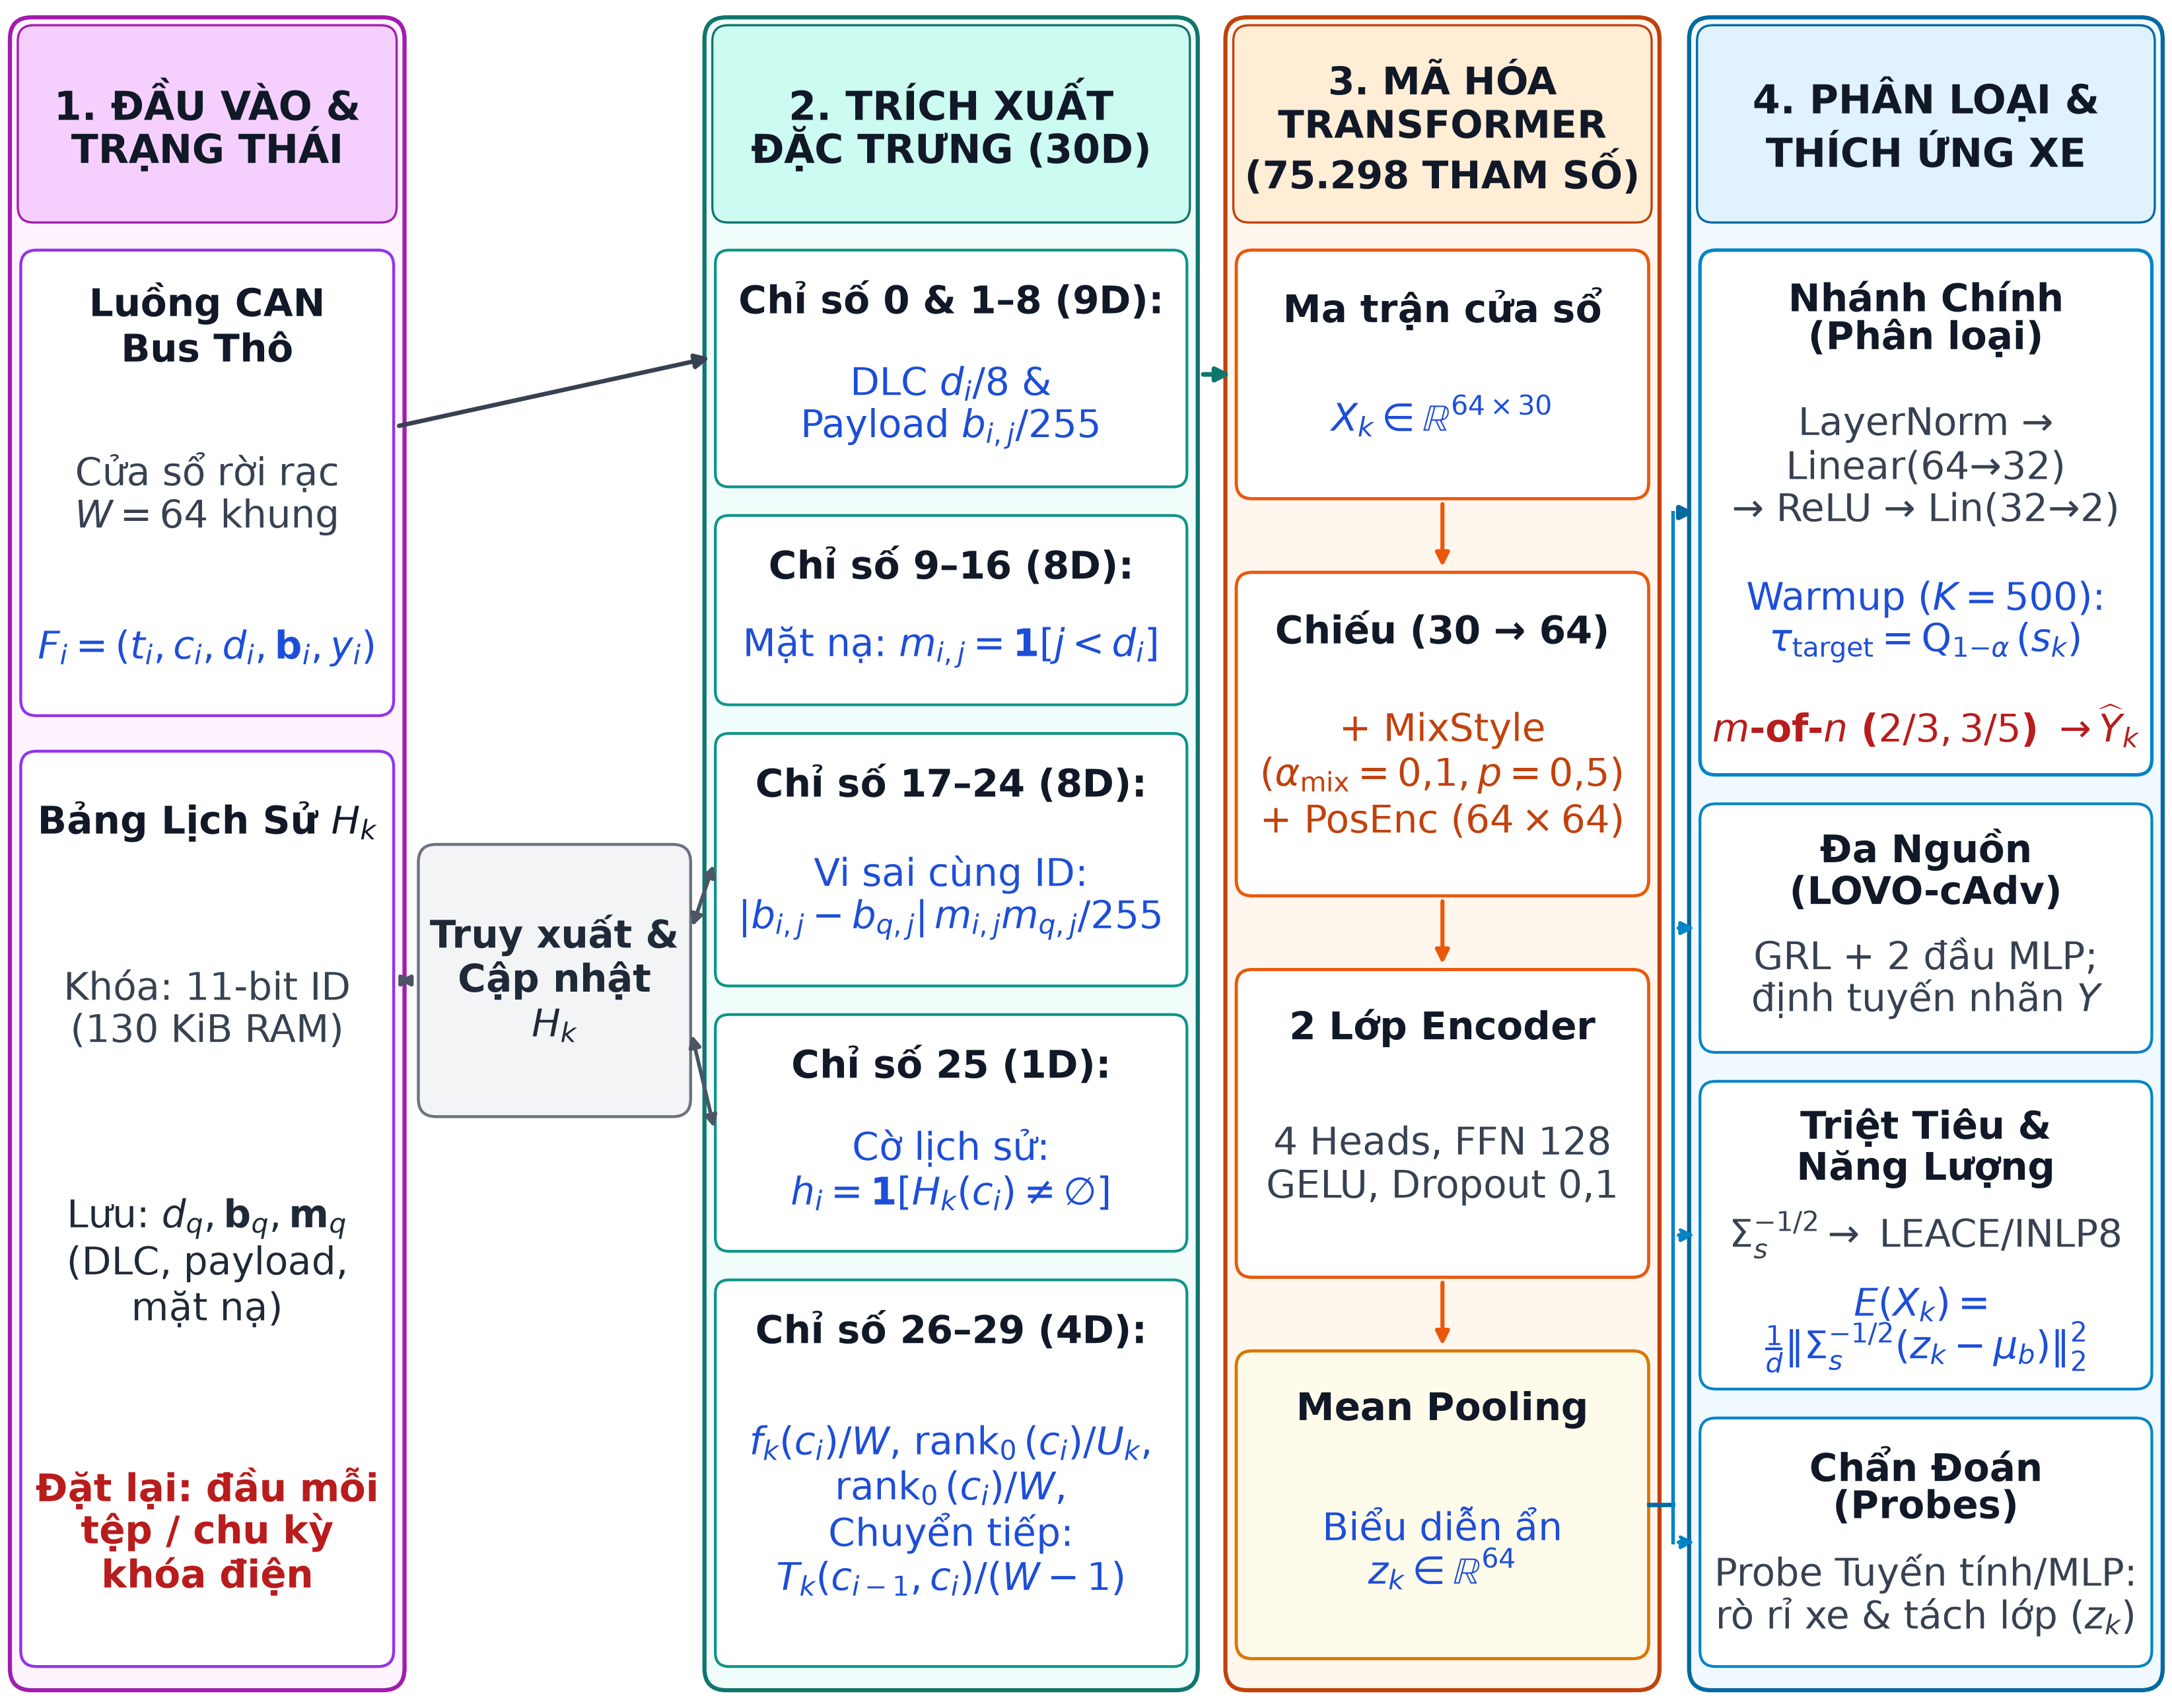
\includegraphics[width=0.98\textwidth]{figs/pipeline_architecture_30d.png}
\caption[Sơ đồ kiến trúc tổng thể Structural Transformer và các nhánh thích ứng]{Sơ đồ kiến trúc tổng thể phương pháp Structural Transformer và các nhánh thích ứng/chẩn đoán: (1) Đầu vào luồng CAN thô ($W=64$) kết hợp cập nhật nhân quả bảng lịch sử $H_k$; (2) Trích xuất vector 30 chiều đặc trưng cấu trúc cấp khung tin; (3) Bộ mã hóa Transformer 2 tầng ($75.298$ tham số) tích hợp MixStyle (tùy chọn trong nhánh thích ứng) và Mean Pooling tạo biểu diễn ẩn cửa sổ $z_k \in \mathbb{R}^{64}$; (4) Nhánh phân loại chính (kèm hiệu chuẩn Benign Warmup $K=500$ và lọc sự kiện $m$-of-$n$) cùng 3 nhánh mở rộng: học đa nguồn LOVO-cAdv DANN, triệt tiêu tuyến tính LEACE/INLP8 với năng lượng Mahalanobis, và bộ thăm dò chẩn đoán rò rỉ danh tính xe.}\label{fig:architecture-30d}
\end{figure}

Cross-entropy ràng buộc dự đoán trên mẫu huấn luyện, không buộc mọi tấn công chưa thấy thuộc lớp bình thường. Điểm thấp ở C/D có thể liên quan tới độ phủ tấn công, biểu diễn, dịch chuyển phân phối hoặc ngưỡng. Do chưa cô lập được hoàn toàn tác động của hàm mục tiêu, không thể quy mọi hạn chế ở Điều kiện C và D cho riêng hàm mất mát cross-entropy hay mặc định rằng việc bổ sung nhánh tái tạo sẽ tự động khắc phục hiện tượng này. Các siêu tham số huấn luyện và ngân sách báo động giả chi tiết của thực nghiệm được trình bày tại Mục~\ref{sec:comparison-protocol} (Bảng~\ref{tab:config}).

{\renewcommand{\arraystretch}{0.9}
\begin{table}[htbp]\centering\footnotesize\setlength{\tabcolsep}{4.5pt}
\caption[Phân loại có hệ thống các cơ chế thích ứng miền và đối chứng bất biến]{Phân loại có hệ thống các cơ chế thích ứng miền và đối chứng bất biến}\label{tab:adaptation-taxonomy}
\begin{tabular}{P{2.6cm}P{2.8cm}P{1.8cm}P{2.4cm}P{1.8cm}P{3.2cm}}
\toprule
Nhóm vai trò & Cơ chế & Dữ liệu nguồn & Ngân sách xe đích & Trọng số mô hình & Nguyên lý cốt lõi\\\midrule
\textbf{Giai đoạn II (Hệ thống chính)} & Hiệu chuẩn tiền tố lành tính \& lọc $m$-trong-$n$ & Đơn nguồn (1 xe) & Tiền tố lành tính không nhãn ($K$ cửa sổ/bản ghi) & Đóng băng hoàn toàn & Ước lượng phân vị ngoại mẫu 1 chiều $\tau_{\text{target}}$ kết hợp lọc sự kiện trượt $m$-trong-$n$\\
\midrule
\textbf{Nhánh chẩn đoán \& đối chứng bất biến} & Điều chuẩn trộn phong cách (MixStyle) & Đơn nguồn (1 xe) & $0$ mẫu đích & Cập nhật khi học & Trộn thống kê $(\mu, \sigma)$ giữa các mẫu cùng nhãn trong từng lô huấn luyện\\
\textbf{Nhánh chẩn đoán \& đối chứng bất biến} & Học đa nguồn đối kháng có điều kiện (LOVO-cAdv) & Đa nguồn (3 xe) & $0$ mẫu đích & Cập nhật đối kháng & Bộ phân biệt miền định tuyến cứng theo nhãn lớp $Y$ kết hợp tầng đảo ngược gradient (GRL)\\
\textbf{Nhánh chẩn đoán \& đối chứng bất biến} & Làm trắng nền lành tính, LEACE/INLP8 \& $E_{\text{white}}$ & Đa nguồn (3 xe) & Tiền tố lành tính đối chứng & Đóng băng (hậu xử lý) & Làm trắng hiệp phương sai nền, triệt tiêu không gian con nhận diện xe và đo năng lượng Mahalanobis\\
\bottomrule\end{tabular}
\end{table}}

\section{Giai đoạn II: Hiệu chuẩn ngưỡng vận hành trên tiền tố lành tính và lọc sự kiện trượt}\label{sec:method-calibration}
Dưới tác động của dịch chuyển hiệp phương sai và dịch chuyển điểm số giữa các dòng xe (Mục~\ref{subsec:domain-shifts}), ngưỡng quyết định đóng băng từ nguồn $\tau_{\text{src}}$ thường bị lệch nghiêm trọng so với phân phối nền lành tính của phương tiện mới. Thay vì tinh chỉnh trọng số mạng nơ-ron --- vốn đòi hỏi dữ liệu tấn công có nhãn trên xe đích và tiềm ẩn nguy cơ quên tri thức nguồn --- Giai đoạn II giữ đóng băng hoàn toàn bộ mã hóa Transformer $f_\theta$ và chỉ thích ứng duy nhất một ngưỡng phân loại vô hướng $\tau_{\text{target}}$ dựa trên một đoạn tiền tố lưu lượng lành tính không nhãn thu thập trên xe đích.

\paragraph{Giao thức xác định tiền tố hợp lệ không rò rỉ:} Gọi $L_{\text{benign}}^{(j)}$ là số cửa sổ lành tính liên tiếp ở đầu bản ghi thứ $j$ trước khi xuất hiện cửa sổ tấn công đầu tiên. Với ngân sách khởi động trần $K \in \{200, 500, 1000\}$ cửa sổ mỗi bản ghi, độ dài tiền tố hợp lệ dùng cho hiệu chuẩn ngoại tuyến được chặn trên bởi:
\begin{equation}
K_{\text{valid}}^{(j)} = \min\left(K, \left\lfloor \frac{L_{\text{benign}}^{(j)}}{2} \right\rfloor\right).
\end{equation}
Ràng buộc $\lfloor L_{\text{benign}}^{(j)} / 2 \rfloor$ đóng vai trò chốt an toàn chống rò rỉ nhãn trong đánh giá ngoại tuyến, bảo đảm đoạn hiệu chuẩn hoàn toàn sạch tấn công đồng thời giữ lại ít nhất một nửa tiền tố lành tính cho tập kiểm thử hậu khởi động. Khi triển khai vật lý trên phương tiện thực tế, $K$ cửa sổ khởi động được thu thập trực tiếp trong pha bật khóa điện / nổ máy tĩnh trước khi xe vận hành.

\paragraph{Ước lượng phân vị gộp đa bản ghi:} Cho tập hợp $J$ bản ghi của cùng một phương tiện đích, hệ thống trích xuất tuần tự các điểm rủi ro vô hướng $s(X_k^{(j)}) = \operatorname{softmax}(f_\theta(X_k^{(j)}))_1$ trên toàn bộ các cửa sổ tiền tố $k \in \{0, \dots, K_{\text{valid}}^{(j)} - 1\}$ và gộp thành đa tập nền $\mathcal{S}_{\text{warm}}$ có tổng kích thước $N_{\text{pool}} = \sum_{j=1}^{J} K_{\text{valid}}^{(j)}$. Tại ngân sách báo động giả danh định $\alpha \in \{0{,}1\%, 0{,}5\%, 1{,}0\%, 2{,}0\%\}$, ngưỡng vận hành trên xe đích được xác định bằng phân vị thực nghiệm:
\begin{equation}
\tau_{\text{target}} = \operatorname{Quantile}_{1-\alpha}(\mathcal{S}_{\text{warm}}).
\end{equation}
Theo phân tích sai số phân vị mẫu hữu hạn (Mục~\ref{subsec:theory-probing-dkw}), để phân vị đuôi tại mức $\alpha$ có ý nghĩa thống kê và không suy biến về giá trị cực đại, cỡ mẫu nền cần thỏa mãn điều kiện $N_{\text{pool}}\alpha \ge 1$. Cơ chế gộp đa phiên giúp thỏa mãn chặt chẽ điều kiện này ngay cả ở ngân sách khắt khe $\alpha = 0{,}1\%$; trong trường hợp triển khai trên một chuyến đi đơn lẻ chỉ có $K = 500$ cửa sổ ($K\alpha = 0{,}5 < 1$ tại $\alpha = 0{,}1\%$), hệ thống cần tích lũy nền qua nhiều chu kỳ khởi động hoặc vận hành ở ngân sách $\alpha \ge 0{,}5\%$ kết hợp bộ lọc sự kiện.

\paragraph{Bộ lọc sự kiện trượt $m$-trong-$n$:} Nhằm triệt tiêu các xung nhiễu báo động giả đơn lẻ trên đường truyền tốc độ cao (1.000--2.000 khung tin/giây), các quyết định nhị phân hậu khởi động ($k \ge K_{\text{valid}}^{(j)}$) đi qua bộ lọc trượt nhân quả:
\begin{equation}\label{eq:mofn-filter}
\hat{Y}_k^{(m/n)} = \mathbf{1}\!\left[\sum_{r = \max(K_{\text{valid}}^{(j)},\, k - n + 1)}^{k} \mathbf{1}\!\left[s(X_r) \ge \tau_{\text{target}}\right] \ge m\right],
\end{equation}
trong đó cảnh báo chính thức chỉ kích hoạt khi có ít nhất $m$ trong tối đa $n$ cửa sổ liên tiếp vượt ngưỡng ($m/n \in \{2/3, 3/5\}$). Về chi phí trực tuyến, bước hiệu chuẩn phân vị chỉ tốn $\mathcal{O}(N_{\text{pool}} \log N_{\text{pool}})$ một lần sau pha khởi động, còn bộ lọc trượt chỉ yêu cầu một bộ đệm vòng kích thước $n$. Toàn bộ quy trình được đặc tả hình thức trong Thuật toán~\ref{alg:benign-cal-mofn}.

\begin{algorithm}[htbp]
\caption{Hiệu chuẩn nền lành tính gộp đa bản ghi ($N_{\text{pool}}$) kết hợp bộ lọc sự kiện trượt $m$-trong-$n$}\label{alg:benign-cal-mofn}
{\small\linespread{1.05}\selectfont
\begin{algorithmic}[1]
\Require Bộ phân loại nguồn đóng băng $f_\theta$; tập hợp $J$ bản ghi của xe đích $\{\mathcal{C}^{(j)}\}_{j=1}^J$ với số cửa sổ lành tính đầu bản ghi $L_{\text{benign}}^{(j)}$; ngân sách khởi động trần mỗi bản ghi $K \in \{200, 500, 1000\}$; ngân sách báo động giả mục tiêu $\alpha \in \{0{,}1\%, 0{,}5\%, 1{,}0\%, 2{,}0\%\}$; tham số lọc trượt $(m, n)$ (mặc định $2/3, 3/5$).
\Ensure Ngưỡng vận hành xe đích $\tau_{\text{target}}$ và chuỗi cảnh báo sự kiện sau khởi động $\{\widehat{Y}_{k, (j)}^{(m/n)}\}$ cho từng bản ghi $j \in \{1, \ldots, J\}$.
\State \textbf{Giai đoạn 1 --- Thu thập điểm nền lành tính gộp đa bản ghi ($N_{\text{pool}}$):}
\State $\mathcal{S}_{\text{warm}} \leftarrow [\,]$ \Comment{Đa tập (multiset) tích lũy điểm số nền lành}
\For{$j = 1$ \textbf{to} $J$}
    \State $K_{\text{valid}}^{(j)} \leftarrow \min\big(K,\, \lfloor L_{\text{benign}}^{(j)} / 2 \rfloor\big)$ \Comment{Ngân sách tiền tố hợp lệ bảo đảm an toàn nhãn}
    \State Khởi tạo trạng thái lịch sử $H_0 \leftarrow \emptyset$ cho bản ghi $j$
    \For{$k = 0$ \textbf{to} $K_{\text{valid}}^{(j)} - 1$}
        \State $X_k^{(j)}, H_{k+1} \leftarrow \Phi(\mathcal{W}_k^{(j)}; H_k)$ \Comment{Trích xuất cấu trúc theo Thuật toán~\ref{alg:causal-30d}}
        \State $s(X_k^{(j)}) \leftarrow \operatorname{softmax}(f_\theta(X_k^{(j)}))_1$ \Comment{Điểm rủi ro từ bộ mã hóa nguồn}
        \State $\mathcal{S}_{\text{warm}} \leftarrow \mathcal{S}_{\text{warm}} \sqcup [s(X_k^{(j)})]$
    \EndFor
\EndFor
\State $N_{\text{pool}} \leftarrow |\mathcal{S}_{\text{warm}}| = \sum_{j=1}^J K_{\text{valid}}^{(j)}$ \Comment{Tổng số cửa sổ nền tích lũy}
\State \textbf{Giai đoạn 2 --- Hiệu chuẩn ngưỡng phân vị thực nghiệm trên xe đích:}
\State $\tau_{\text{target}} \leftarrow \operatorname{Quantile}_{1-\alpha}(\mathcal{S}_{\text{warm}})$ \Comment{Bảo đảm điều kiện cỡ mẫu đuôi $N_{\text{pool}}\alpha \ge 1$}
\State \textbf{Giai đoạn 3 --- Suy luận hậu khởi động và lọc sự kiện trượt $m$-trong-$n$ trên từng bản ghi:}
\For{$j = 1$ \textbf{to} $J$}
    \For{$k = K_{\text{valid}}^{(j)}$ \textbf{to} $M^{(j)} - 1$}
        \State $X_k^{(j)}, H_{k+1} \leftarrow \Phi(\mathcal{W}_k^{(j)}; H_k)$
        \State $s(X_k^{(j)}) \leftarrow \operatorname{softmax}(f_\theta(X_k^{(j)}))_1$
        \State $a_k \leftarrow \mathbf{1}\big[s(X_k^{(j)}) \ge \tau_{\text{target}}\big]$ \Comment{Quyết định nhị phân thô tại cửa sổ $k$}
        \State $j_0 \leftarrow \max(K_{\text{valid}}^{(j)},\, k - n + 1)$
        \State $\widehat{Y}_{k, (j)}^{(m/n)} \leftarrow \mathbf{1}\left[\sum_{r=j_0}^{k} a_r \ge m\right]$ \Comment{Phát cảnh báo khi có $\ge m$ trên $n$ cửa sổ vượt ngưỡng}
    \EndFor
\EndFor
\State \Return $\tau_{\text{target}}, \{\widehat{Y}_{k, (j)}^{(m/n)}\}$
\end{algorithmic}}
\end{algorithm}

\section{Các cơ chế thích ứng và triệt tiêu cấp đặc trưng phục vụ chẩn đoán bất biến miền}\label{sec:domain-adaptation-methods}
Bên cạnh cơ chế hiệu chuẩn ngưỡng ở đầu ra (Giai đoạn II), một câu hỏi lý thuyết trọng tâm là liệu có thể triệt tiêu trực tiếp dấu ấn đặc thù xe ngay trong không gian biểu diễn tiềm ẩn $z_k \in \mathbb{R}^{64}$ hay không (Câu hỏi nghiên cứu RQ5b). Để kiểm định giả thuyết này một cách hệ thống và đối chứng với Giai đoạn II, khóa luận tích hợp ba nhóm phương pháp thích ứng và triệt tiêu cấp đặc trưng (tổng hợp tại nửa dưới Bảng~\ref{tab:adaptation-taxonomy}).

\subsection{Điều chuẩn phân phối ẩn bằng trộn phong cách (MixStyle)}\label{subsec:method-mixstyle}
Nhằm tăng cường sức chống chịu trước biến thiên phân phối đầu vào ngay từ pha huấn luyện đơn nguồn mà không cần dữ liệu xe đích, kỹ thuật MixStyle~\cite{zhou2021mixstyle} được thích ứng cho chuỗi thời gian CAN. Sau tầng chiếu tuyến tính ($E \in \mathbb{R}^{W \times d}, d = 64$) và trước khi cộng mã hóa vị trí, với mỗi cặp mẫu cùng nhãn $(X, \widetilde{X})$ trong cùng lô huấn luyện ($Y = \widetilde{Y}$), thống kê kỳ vọng $\mu(X)$ và độ lệch chuẩn $\sigma(X)$ theo trục khung tin:
\begin{equation}
\mu(X) = \frac{1}{W}\sum_{i=1}^W E_i, \qquad \sigma(X) = \sqrt{\frac{1}{W}\sum_{i=1}^W (E_i - \mu(X))^2 + \epsilon}.
\end{equation}
Thống kê phong cách hỗn hợp được tạo qua phép nội suy lồi với hệ số $\lambda \sim \operatorname{Beta}(\alpha_{\text{mix}}, \alpha_{\text{mix}})$ ($\alpha_{\text{mix}} = 0{,}1$):
\begin{align}
\gamma &= \lambda \sigma(X) + (1 - \lambda) \sigma(\widetilde{X}),\\
\beta &= \lambda \mu(X) + (1 - \lambda) \mu(\widetilde{X}),
\end{align}
để tạo thống kê hỗn hợp $(\beta, \gamma)$ và chuẩn hóa lại theo công thức:
\begin{equation}
\operatorname{MixStyle}(X) = \gamma \odot \frac{E - \mu(X)}{\sigma(X)} + \beta.
\end{equation}
Phép trộn chỉ kích hoạt ngẫu nhiên với xác suất $p = 0{,}5$ lúc huấn luyện; trong pha suy luận, nhánh này trở về ánh xạ đồng nhất thuần túy nên không phát sinh bất kỳ chi phí tính toán bổ sung nào.

\subsection{Học đa nguồn giữ ngoài một xe kết hợp đối kháng có điều kiện (LOVO-cAdv)}\label{subsec:method-lovo}
Khi dữ liệu huấn luyện có sẵn từ nhiều dòng xe nguồn, khóa luận thiết lập giao thức học đa nguồn giữ ngoài một xe (\textit{Leave-One-Vehicle-Out} --- LOVO) trên bốn dòng xe vật lý (Impala, Traverse, Silverado và Forester): mỗi lượt kiểm thử giữ trọn một xe làm miền đích chưa quan sát và dùng ba xe còn lại làm miền nguồn tách biệt theo mã băm SHA-256.

Kiến trúc mạng đối kháng miền (DANN~\cite{ganin2016dann}) gồm bộ trích xuất đặc trưng $G_f$, bộ phân loại tấn công $G_y$ và bộ phân biệt miền đối kháng có điều kiện $G_d$. Để tránh ép xóa nhầm các đặc trưng phân tách lớp tấn công, $G_d$ gồm hai đầu mạng MLP 2 tầng độc lập $G_{d,0}$ và $G_{d,1}$ được định tuyến cứng theo nhãn lớp thực $Y \in \{0, 1\}$ của mẫu nguồn, nối với $z_k = G_f(X_k)$ qua tầng đảo ngược gradient ($\text{GRL}_\lambda$) với hệ số $\lambda(p) = \frac{2}{1 + \exp(-10p)} - 1$ theo hàm mục tiêu:
\begin{equation}
\mathcal{L}_{\text{total}} = \mathcal{L}_y(G_y(z_k), Y) - \lambda \mathcal{L}_d(G_d(z_k), D),
\end{equation}
trong đó $D$ là nhãn định danh miền xe nguồn. Song song với đầu vào cấu trúc 30 chiều đầy đủ (\textit{Structural + cAdv}), khóa luận khảo sát thêm biến thể lược bỏ 8 byte payload tuyệt đối (\textit{Relative + cAdv}, 22 chiều --- chỉ giữ DLC, mặt nạ hiệu lực, vi sai $\Delta\text{payload}$, cờ lịch sử $h_i$ và các thống kê cục bộ) nhằm buộc bộ mã hóa tập trung hoàn toàn vào quy luật biến thiên tương đối.

\subsection{Làm trắng nền lành tính, triệt tiêu khái niệm tuyến tính (LEACE/INLP8) và điểm năng lượng Mahalanobis}\label{subsec:method-whitening}
Nhằm chẩn đoán trực tiếp mức độ tồn lưu thông tin nhận diện phương tiện và ranh giới giữa bất biến tuyến tính với rò rỉ phi tuyến trên biểu diễn ẩn đóng băng $z_k \in \mathbb{R}^{64}$, khóa luận thiết lập chuỗi hậu xử lý gồm ba bước:
\begin{enumerate}
    \item \textbf{Làm trắng hiệp phương sai nền lành tính:} Từ tập cửa sổ lành tính đối chứng thu thập trên xe đích (gồm 2.000 cửa sổ tách làm hai tập con 1.000 cửa sổ ước lượng tham số và 1.000 cửa sổ chọn ngưỡng), hệ thống tính vector kỳ vọng $\mu_b$ và ma trận hiệp phương sai chính quy hóa co $\Sigma_s = (1 - \gamma)\Sigma_b + \gamma\bar{\sigma}^2 I$ ($\gamma = 0{,}1$), rồi áp dụng phép biến đổi làm trắng $W_{\text{white}} = \Sigma_s^{-1/2}$ để đưa phân phối nền của từng xe về kỳ vọng triệt tiêu và hiệp phương sai đơn vị: $z'_k = W_{\text{white}}(z_k - \mu_b)$. (Lưu ý về thiết kế tách tập chẵn--lẻ so với chia khối thời gian liên tục sẽ được đánh giá đối chứng cụ thể trong Chương~\ref{chap:results}).
    \item \textbf{Triệt tiêu khái niệm tuyến tính:} Áp dụng phép chiếu xiên dạng đóng LEACE~\cite{belrose2023leace} ($P = I - \Sigma_X^{1/2}UU^\top \Sigma_X^{-1/2}$, trực giao dưới tích vô hướng Mahalanobis $\Sigma_X^{-1}$) hoặc phép chiếu không gian rỗng lặp INLP~\cite{ravfogel2020null} (lặp tối đa 32 vòng để rút gọn về 8 chiều dư, ký hiệu INLP8) ước lượng trên các xe nguồn nhằm xóa triệt để mọi hướng tuyến tính mang thông tin nhận diện hãng xe.
    \item \textbf{Điểm bất thường năng lượng Mahalanobis ($E_{\text{white}}$):} Tính khoảng cách bình phương trung bình chuẩn hóa trên không gian đã làm trắng (theo khoảng cách Mahalanobis~\cite{lee2018mahalanobis}) mà không phụ thuộc vào đầu phân loại nhị phân nguồn:
    \begin{equation}
    E_{\text{white}}(X_k) = \frac{1}{d}\left\|W_{\text{white}}(z_k - \mu_b)\right\|_2^2 \quad (d = 64).
    \end{equation}
\end{enumerate}

\section{Tóm tắt chương}\label{sec:method-summary}
Chương~\ref{chap:method} đã phát biểu hình thức bài toán phát hiện xâm nhập mạng CAN xuyên phương tiện và đặc tả trọn vẹn khung giải pháp đề xuất gồm hai giai đoạn cốt lõi: \textbf{Giai đoạn I} xây dựng không gian biểu diễn cấu trúc 30 chiều độc lập định danh (cùng nhánh mở rộng động học thời gian 32 chiều cho bus đồng hồ chuẩn) kết hợp bộ mã hóa Transformer 75.298 tham số; \textbf{Giai đoạn II} bổ sung cơ chế hiệu chuẩn phân vị trên tiền tố lành tính không nhãn kết hợp bộ lọc sự kiện trượt $m$-trong-$n$ nhằm khôi phục điểm vận hành mà không huấn luyện lại mô hình. Bên cạnh đó, chương đã trình bày hệ thống các phương pháp thích ứng và triệt tiêu cấp đặc trưng (MixStyle, LOVO-cAdv, làm trắng nền lành tính, LEACE/INLP8 và $E_{\text{white}}$) làm công cụ đối chứng lý thuyết cho hiện tượng đan xen đặc trưng. Chương~\ref{chap:results} sẽ triển khai đánh giá thực nghiệm toàn diện khung đề xuất và các nhánh đối chứng này theo năm câu hỏi nghiên cứu RQ1--RQ5.

\chapter{Thực nghiệm và đánh giá}\label{chap:results}
Chương này triển khai hệ thống thực nghiệm đối chứng đa phương tiện diện rộng nhằm kiểm chứng thực nghiệm các giả thuyết khoa học và trả lời trọn vẹn năm câu hỏi nghiên cứu (RQ1--RQ5) đã xác lập ở phần Mở đầu. Bố cục chương và bản đồ ánh xạ câu hỏi nghiên cứu được tổ chức như sau:
\begin{itemize}
    \item \textbf{Mục~\ref{sec:comparison-protocol} (Thiết lập và giao thức thực nghiệm):} Trình bày quy tắc chia tách dữ liệu, lấy mẫu reservoir, cấu hình siêu tham số và hệ thống độ đo kiểm định.
    \item \textbf{Mục~\ref{sec:zeroshot-eval} (Đánh giá chuyển giao zero-shot và chẩn đoán biểu diễn):}
    \begin{itemize}
        \item \textit{Mục~\ref{sec:comparison-results} \&~\ref{subsec:timed-vs-content}:} Trả lời \textbf{RQ1} về hiệu năng chuyển giao phương tiện và sự phân kỳ giữa chất lượng xếp hạng độc lập ngưỡng (AP) với độ nhạy tại ngưỡng tĩnh, cùng vai trò của động học thời gian.
        \item \textit{Mục~\ref{sec:completion}:} Trả lời \textbf{RQ2} về đóng góp của từng nhóm thành phần đặc trưng (cú pháp, vi sai $\Delta\text{payload}$, thống kê cục bộ) và độ nhạy kích thước cửa sổ $W$.
        \item \textit{Mục~\ref{sec:eval-probes}:} Trả lời \textbf{RQ3} về hiện tượng đan xen đặc trưng và giới hạn của tính bất biến biểu diễn thông qua thăm dò tuyến tính có kiểm soát.
        \item \textit{Mục~\ref{sec:eval-external}:} Trả lời \textbf{RQ4} về năng lực tổng quát hóa ngoại bộ trên ba bộ dữ liệu độc lập và ranh giới thất bại thực tế.
    \end{itemize}
    \item \textbf{Mục~\ref{sec:adaptation-eval} (Đánh giá các cơ chế thích ứng miền và khôi phục điểm vận hành):}
    \begin{itemize}
        \item \textit{Mục~\ref{sec:benign-calibration}:} Trả lời \textbf{RQ5a} về khôi phục điểm vận hành qua hiệu chuẩn tiền tố lành tính không giám sát ($K=500$, lọc trượt $m$-trong-$n$) và lợi thế tham số so với mô hình thuần đích.
        \item \textit{Mục~\ref{sec:feature-invariance}:} Trả lời \textbf{RQ5b} về giới hạn của các kỹ thuật thích ứng và triệt tiêu cấp đặc trưng (MixStyle, LOVO-cAdv, làm trắng nền lành tính và LEACE/INLP8).
    \end{itemize}
    \item \textbf{Mục~\ref{sec:runtime} \&~\ref{sec:threats-to-validity}:} Phân tích chi phí tính toán, độ trễ thời gian thực và thảo luận các mối đe dọa tính hợp lệ.
\end{itemize}

\section{Thiết lập và giao thức thực nghiệm}
\subsection{Tách nguồn, lấy mẫu reservoir và chống rò rỉ}
Bảng~\ref{tab:split-stats} tổng hợp cấu trúc chia tách theo hậu tố vòng ghi (\textit{recording round}) trên 4 tập dữ liệu sau kiểm tra toàn vẹn đầu vào: tổng cộng 30 tệp huấn luyện nguồn (388.435 cửa sổ W64 khả dụng; hậu tố 1 ở Set 1--2 và hậu tố 3 ở Set 3--4) và 30 tệp validation nguồn (385.168 cửa sổ W64 đầy đủ không cắt tỉa; hậu tố 2 ở Set 1--2 và hậu tố 4 ở Set 3--4), tách biệt hoàn toàn khỏi tập kiểm thử A--D trong cả pha học và chọn ngưỡng.

{\renewcommand{\arraystretch}{0.88}
\begin{table}[htbp]\centering\footnotesize
\caption{Thống kê chia tách tập huấn luyện/validation nguồn, số lượng tệp kiểm thử và phân bố họ tấn công trên bốn tập \texttt{can-train-and-test}}\label{tab:split-stats}
\begin{tabular}{P{1.1cm}P{2.2cm}P{2.2cm}P{1.5cm}P{6.3cm}}
\toprule
Set & Nguồn (Train/Val) & Test A/B/C/D & Hậu tố Val & Họ tấn công trong A--B / C--D \\ \midrule
1 & 6 / 6 tệp & 8 / 8 / 12 / 12 & 2 & A--B: DoS, force-neutral, rpm, standstill; C--D: double, fuzzing, interval, speed, systematic, triple \\
2 & 8 / 8 tệp & 12 / 12 / 8 / 8 & 2 & A--B: double, fuzzing, interval, speed, systematic, triple; C--D: DoS, force-neutral, rpm, standstill \\
3 & 7 / 7 tệp & 10 / 10 / 14 / 14 & 4 & A--B: DoS, double, force-neutral, fuzzing, triple; C--D: interval, rpm, rpm-acc., speed, speed-acc., standstill, systematic \\
4 & 9 / 9 tệp & 14 / 14 / 10 / 10 & 4 & A--B: interval, rpm, rpm-acc., speed, speed-acc., standstill, systematic; C--D: DoS, double, force-neutral, fuzzing, triple \\
\bottomrule
\end{tabular}
\end{table}}

Về quy tắc chia tách và lọc tệp trên các bộ dữ liệu nghiên cứu: đối với \textit{can-train-and-test}, tập validation nguồn được tách theo hậu tố vòng ghi độc lập, tuyệt đối không can thiệp vào tập kiểm thử chính thức; đối với \textit{Automotive v2}, nhãn tấn công DoS được xác định nghiêm ngặt theo khoảng cách thời gian và chữ ký khung tin thay vì gán nhãn thô toàn bộ tệp; đối với \textit{CAN-MIRGU}, toàn bộ khung tin được đồng bộ nhãn từ nhật ký tấn công và kiểm tra tính toàn vẹn; đối với \textit{CICIoV2024}, thực nghiệm tuân thủ giao thức thứ tự hàng trong tệp CSV do không có dấu thời gian đo lường; và bộ dữ liệu \textit{OTIDS} chưa đưa vào kết luận chính thức do cần xác minh tính nhất quán nhãn sau chuyển đổi. Các tệp nguồn được gom theo hậu tố vòng ghi (nhóm hậu tố lớn nhất làm validation; không tái huấn luyện trên tập validation sau khi chốt ngưỡng). Việc lấy mẫu huấn luyện áp dụng thuật toán random-priority reservoir theo từng tệp và lớp (tối đa $1.000$ cửa sổ/lớp/tệp với \code{sampling\_seed=20261103}) trên luồng đã trích xuất trạng thái liên tục; mọi phương pháp dùng chung đúng bộ chỉ số mẫu nguồn này, trong khi tập validation và kiểm thử A--D được đánh giá đầy đủ với tỷ lệ lớp nguyên bản.

\noindent\textbf{Dịch chuyển tiên nghiệm lớp từ lấy mẫu reservoir và lộ trình đánh giá hai giai đoạn:} Việc áp trần lấy mẫu $1.000$ cửa sổ/lớp/tệp trên tập huấn luyện nguồn tạo ra phân bố lớp nhân tạo tiệm cận cân bằng ($50:50$). Ngược lại, phân bố tấn công thực tế trên các tập kiểm thử A--D biến thiên hơn ba bậc độ lớn, phổ biến trong khoảng $0{,}03\%\text{--}8{,}0\%$ (và có thể đạt $97\%$ ở các tệp DoS/interval, xem thống kê tại Mục~\ref{subsec:bd-per-file-counts}). Sự dịch chuyển tiên nghiệm lớp (\textit{class-prior shift}) giữa pha huấn luyện và kiểm thử này là yếu tố nhiều khả năng thúc đẩy hiện tượng bão hòa logit (\textit{logit saturation}) của tầng phân loại softmax, đồng thời khuếch đại độ nhạy và phương sai chọn ngưỡng cực đoan giữa các hạt giống khởi tạo (như hiện tượng sụp đổ ngưỡng ở Set~1 seed 42 so với seed 43--44). Để khảo sát hiện tượng này một cách khoa học và minh bạch, lộ trình đánh giá của khóa luận được phân định thành hai giai đoạn rõ rệt: \textbf{Giai đoạn 1 (Mục~\ref{sec:zeroshot-eval})} kiểm chứng nghiêm ngặt giả thuyết zero-shot dưới ngưỡng tĩnh đóng băng từ nguồn trên cả bốn điều kiện A--D và 57 bản ghi ngoại bộ; \textbf{Giai đoạn 2 (phương pháp tại Mục~\ref{sec:domain-adaptation-methods}, thực nghiệm tại Mục~\ref{sec:adaptation-eval})} nghiên cứu khôi phục điểm vận hành bằng hiệu chuẩn nền lành tính không giám sát và đối chứng trực diện với các bộ phát hiện thuần không giám sát trên xe đích (Target-Only). Mỗi lượt thực nghiệm đều kiểm tra tính toàn vẹn SHA-256, lược đồ bốn tập và phát hiện tệp trùng lặp, lưu ý rằng mã băm chỉ xác nhận toàn vẹn tệp chứ chưa tự chứng minh các vòng ghi độc lập hoàn toàn về mặt chuyến lái.

\subsection{Đối chứng, cấu hình huấn luyện và giao thức so sánh CTT}\label{sec:comparison-protocol}
Bảng~\ref{tab:config} tóm tắt các siêu tham số huấn luyện mặc định và ngân sách báo động giả validation dùng để chọn ngưỡng nguồn ($100/100.000$ cửa sổ lành, đóng vai trò điểm chuẩn so sánh chứ không phải chuẩn an toàn ô tô). Hồi quy logistic (LR) chỉ dùng cho phân tích probe hậu nghiệm, không xếp hạng như một bộ IDS.

{\renewcommand{\arraystretch}{0.88}
\begin{table}[htbp]\centering\footnotesize
\caption{Các siêu tham số huấn luyện và ngân sách báo động giả mặc định của thực nghiệm}\label{tab:config}
\begin{tabular}{P{6.5cm}P{6.5cm}}
\toprule
Tham số & Giá trị \\
\midrule
Cửa sổ chính / độ nhạy & 64 / 32 và 128\\
Hidden / layers / heads & 64 / 2 / 4\\
Feed-forward / dropout & 128 / 0,1\\
Optimizer & AdamW\\
Learning rate / weight decay & 0,001 / $10^{-4}$\\
Epochs / batch size & 10 / 128\\
Scheduler & Cosine theo epoch\\
Seed khởi tạo & 42, 43, 44\\
Seed lấy mẫu chung & 20261103\\
Giới hạn mỗi file, mỗi lớp train & 1.000 cửa sổ\\
Ngân sách FAR validation & 100/100.000 cửa sổ benign\\
\bottomrule
\end{tabular}
\end{table}}

\textbf{Giao thức chuẩn hóa theo thứ tự nội dung bản ghi (đối sánh thuần nội dung):} Quét toàn bộ 236 tệp CTT ghi nhận 193.240.845 khung dữ liệu (chênh 236 dòng tiêu đề so với 193.241.081 dòng CSV), 3.019.271 cửa sổ $W=64$ toàn kho và 12.527 lần dấu thời gian đi lùi trên 100 tệp. Do đó, ma trận chính gồm 60 đơn vị IDS (4 set $\times$ 3 seed $\times$ 5 phương pháp) chỉ sử dụng nhánh nội dung theo thứ tự tệp (Raw 28D và Structural 30D; mã băm SHA-256 lưu tại Phụ lục~\ref{sec:app-provenance}), tách riêng nhánh Timed (29D/32D) sang đối chứng độc lập trên 136 tệp đơn điệu tại Mục~\ref{subsec:timed-vs-content} (Chương~\ref{chap:results}).

\subsubsection{Đối thủ, supervision và thay đổi so với công bố}
Raw và Structural Transformer dùng chung thân bộ mã hóa, mẫu nguồn, CE/AdamW/Cosine (10 epoch, batch 128), chỉ khác biểu diễn đầu vào 28/30 chiều. Ba phương pháp đối thủ được thích ứng chuẩn hóa trên cùng tập mẫu nguồn và đơn vị cửa sổ $W=64$ (commit Git ghim tại Phụ lục~\ref{sec:app-provenance}):
\begin{itemize}
    \item \textbf{\code{CANBERT+ adapted}~\cite{won2026canbertplus}:} Kiến trúc BERT/MLM (hidden 768, 6 tầng, 12 head) tiền huấn luyện masked-ID 15\% trên nền lành nguồn 3 epoch và tinh chỉnh nhãn khung tin 3 epoch (batch 8, vòng lặp PyTorch), gộp điểm cửa sổ bằng $\max_{i\in\mathcal{W}_k} s_i$. Phép gộp cực đại này nhạy với ngoại lệ đơn lẻ, dễ ép ngưỡng nguồn về biên cực đoan (như Set~1 seed 42 ngưỡng suy biến về $8{,}34\times 10^{-16}$, gây FAR $99{,}84\%$ ở B) hoặc sụp đổ recall ở Điều kiện A ($0{,}3843$).
    \item \textbf{\code{CANLP-char-DNN adapted}~\cite{balasubramanian2025canlp}:} Đặc trưng TF-IDF ký tự (unigram, tối đa 256 bigram) + ID/2048 qua Dense 128/64 (dropout 0,15, 30 epoch, Adam 0,001, batch 512), gộp điểm cực đại theo $W=64$.
    \item \textbf{\code{CrySyS-AssocRules/W64}~\cite{koltai2026trust}:} Khai phá luật kết hợp trên nền lành nguồn với $W=64$/stride $64$ ($k=300$, ngưỡng khoảng cách $0{,}3$, itemset tối đa 3/2) qua backend cache khớp chính xác từng phép tính (kiểm thử pilot $k=2$ xác nhận trùng khớp tuyệt đối và tăng tốc $\sim 8{,}3\times$). Do thưa mẫu train và cửa sổ ngắn $W=64$, tỷ lệ cửa sổ validation đạt điểm $1{,}0$ vượt ngân sách $100/100\text{k}$, đẩy ngưỡng nguồn lên $1 + \varepsilon_{\text{mach}} \approx 1{,}0000000000000002$ (chuẩn IEEE 754 64-bit, đẩy toàn bộ dự đoán về lớp lành tính: $R=0, \text{FAR}=0$).
\end{itemize}
Vì các phương pháp khác nhau về dạng giám sát (cửa sổ, khung tin, chỉ nền lành) và dung lượng tham số, đây là đối sánh quy trình trên cùng dữ liệu/ngưỡng chứ không phải ablation cùng ngân sách. Các kết quả Set~1/seed 42 dùng lại sau kiểm tra đồng nhất hash và cấu hình; cơ chế song song GPU có thể gây sai số bất định nhỏ theo phần cứng.

\subsection{Ngưỡng quyết định, hệ thống độ đo và thiết kế kiểm định}
Ngưỡng hiệu chuẩn nguồn tối đa hóa recall validation dưới ngân sách $\text{FAR} \le 100/100\text{k}$ (hòa chọn ít FP hơn rồi ngưỡng cao hơn; các điểm bằng nhau xử lý cùng nhóm; nếu không thỏa thì đặt trên điểm cực đại để dự đoán toàn benign). Với $N_+=TP+FN$ và $N_-=TN+FP$:
\begin{align}
P&=TP/(TP+FP), & R&=TP/N_+,\\
F_1&=2TP/(2TP+FP+FN), & \operatorname{FAR}_{100k}&=10^5FP/N_-.
\end{align}
Khi $N_-=0$, FAR là N/A; khi thiếu lớp dương hoặc không cảnh báo, xử lý theo quy ước chuẩn và không thay AP (tính từ điểm liên tục) bằng F1. Độ phân giải FAR thực nghiệm nhỏ nhất là $10^5/N_-$. Trong phép so ghép cặp (Structural trừ đối thủ cùng set/seed), kết quả được trung bình theo 3 seed trong từng set rồi gán trọng số đều 4 set (và đối chiếu thêm trung bình 3 xe đích khử lặp); khoảng bootstrap ghép cặp 1.000 mẫu lấy lại toàn bộ capture file là mô tả có điều kiện trên tệp quan sát chứ không phải CI quần thể xe.

Nhằm bóc tách có hệ thống đóng góp của từng thành phần biểu diễn và cô lập các kênh gây rò rỉ thông tin xe, nghiên cứu thiết lập ma trận gồm 10 biến thể cắt bỏ đối chứng cùng các kiểm định độ nhạy kích thước cửa sổ và thăm dò tuyến tính có kiểm soát (chi tiết ma trận đối chứng và mục tiêu kiểm định tương ứng được tổng hợp tại Bảng~\ref{tab:ablations}, Phụ lục~\ref{app:sensitivity}). Để đo mức độ tồn lưu thông tin xe và tấn công, nghiên cứu chạy \textit{Linear Probe} (bộ phân loại hồi quy logistic với $C=1$, tối đa 2.000 vòng lặp) trên các biểu diễn ẩn đóng băng với tập chẩn đoán chia theo vòng ghi và cân bằng ô xe $\times$ nhãn (mức cơ hội đoán xe $1/V=0{,}25$), kèm ba đối chứng kiểm soát Hewitt--Liang~\cite{hewitt2019probes} (embedding hằng số, nhiễu Gaussian độc lập và hoán vị nhãn huấn luyện qua 5 hạt giống cố định).

\subsection{Môi trường tính toán và cơ chế đảm bảo tái lập}
Mỗi lượt chạy lưu đầy đủ tệp cấu hình, mã băm SHA-256 dữ liệu, điểm kiểm tra mô hình và tệp dự đoán, đồng thời khóa ghi đè thư mục hoàn tất và chạy lại từ đầu các lượt bị gián đoạn. Phép đo thời gian xử lý thực hiện trên máy trạm AMD Ryzen 5 5600X (16 GB RAM) và GPU NVIDIA GeForce RTX 5060 (8 GB VRAM, Windows 11) với \code{batch=1} (20 cửa sổ khởi động, 300 cửa sổ $\times$ 3 lần = 900 mẫu), phản ánh chi phí tính toán thí nghiệm (chưa bao gồm $32\text{--}64\text{ ms}$ chờ gom cửa sổ và không thay thế kiểm định deadline ECU nhúng).

\section{Đánh giá chuyển giao zero-shot và chẩn đoán biểu diễn cấu trúc}\label{sec:zeroshot-eval}
\subsection{Đánh giá hiệu năng phát hiện và báo động giả khi chuyển giao phương tiện (RQ1)}\label{sec:comparison-results}
Kết quả đối sánh chi tiết nhằm trả lời câu hỏi nghiên cứu RQ1 được phân tích có hệ thống dưới đây. Bảng~\ref{tab:comparison-main} báo cáo kết quả đối sánh chính của năm phương pháp tại kích thước cửa sổ $W=64$ dưới ngưỡng đóng băng từ nguồn qua bốn điều kiện chuyển giao A--D (thống kê mẫu số cửa sổ kiểm thử chi tiết tại Bảng~\ref{tab:comparison-counts}, và chi tiết chênh lệch hiệu năng ghép cặp đối chứng tại Bảng~\ref{tab:comparison-paired}, Phụ lục~\ref{app:sensitivity}).

\Needspace{6\baselineskip}
{\footnotesize\renewcommand{\arraystretch}{0.85}
\begin{longtable}{P{1.0cm}P{4.4cm}P{1.4cm}P{3.0cm}P{1.4cm}P{1.4cm}}
\caption[Kết quả đối sánh chính năm phương pháp ở cửa sổ $W=64$ dưới ngưỡng nguồn]{Kết quả đối sánh chính của năm phương pháp tại kích thước cửa sổ $W=64$ dưới ngưỡng đóng băng từ nguồn qua bốn điều kiện A--D (FAR tính trên $100.000$ cửa sổ lành tính kèm tỷ lệ phần trăm tương đương)}\label{tab:comparison-main}\\\toprule
ĐK & Phương pháp & Recall & FAR /100k (\%) & F1 & AP\\\midrule
\endfirsthead\caption[]{(tiếp theo)}\\\toprule
ĐK & Phương pháp & Recall & FAR /100k (\%) & F1 & AP\\\midrule
\endhead
A & Raw TF & 0,6167 & 115,77 (0,12\%) & 0,7258 & 0,7312\\
A & Structural TF & 0,5886 & 81,67 (0,08\%) & 0,7072 & 0,7483\\
A & CANBERT+ adapted & 0,3843 & 79,27 (0,08\%) & 0,4576 & 0,5335\\
A & CANLP-char-DNN adapted & 0,1228 & 28,37 (0,03\%) & 0,1789 & 0,5482\\
A & CrySyS-AssocRules/W64$^{\dagger}$ & 0,0000 & 0,00 (0,00\%) & 0,0000 & 0,3338\\
B & Raw TF & 0,8541 & 65301,41 (65,30\%) & 0,3000 & 0,3781\\
B & Structural TF & 0,7383 & 52461,46 (52,46\%) & 0,2435 & 0,5554\\
B & CANBERT+ adapted & 0,6395 & 64843,85 (64,84\%) & 0,0593 & 0,0970\\
B & CANLP-char-DNN adapted & 0,2854 & 29695,88 (29,70\%) & 0,0329 & 0,0542\\
B & CrySyS-AssocRules/W64$^{\dagger}$ & 0,0000 & 0,00 (0,00\%) & 0,0000 & 0,0591\\
C & Raw TF & 0,2101 & 91,92 (0,09\%) & 0,2314 & 0,2661\\
C & Structural TF & 0,2230 & 75,82 (0,08\%) & 0,2600 & 0,2928\\
C & CANBERT+ adapted & 0,1037 & 62,54 (0,06\%) & 0,1461 & 0,2218\\
C & CANLP-char-DNN adapted & 0,0020 & 405,49 (0,41\%) & 0,0038 & 0,2373\\
C & CrySyS-AssocRules/W64$^{\dagger}$ & 0,0000 & 0,00 (0,00\%) & 0,0000 & 0,1732\\
D & Raw TF & 0,6614 & 67982,89 (67,98\%) & 0,1213 & 0,1648\\
D & Structural TF & 0,6445 & 54643,37 (54,64\%) & 0,2069 & 0,3357\\
D & CANBERT+ adapted & 0,5549 & 54513,45 (54,51\%) & 0,0644 & 0,1311\\
D & CANLP-char-DNN adapted & 0,2491 & 25452,19 (25,45\%) & 0,0119 & 0,0901\\
D & CrySyS-AssocRules/W64$^{\dagger}$ & 0,0000 & 0,00 (0,00\%) & 0,0000 & 0,0912\\
\bottomrule
\multicolumn{6}{P{13.4cm}}{\footnotesize $^{\dagger}$ Ngưỡng chọn từ validation nguồn suy biến tại $1 + \varepsilon_{\text{mach}} > 1{,}0$ (giá trị máy $1{,}0000000000000002$, dự đoán toàn bộ là benign: $R=0, \text{FAR}=0$); xem chi tiết ở Mục~\ref{subsec:assoc-degenerate}.}
\end{longtable}}



\begin{figure}[htbp]
\centering
\begin{subfigure}[b]{0.45\textwidth}
  \centering
  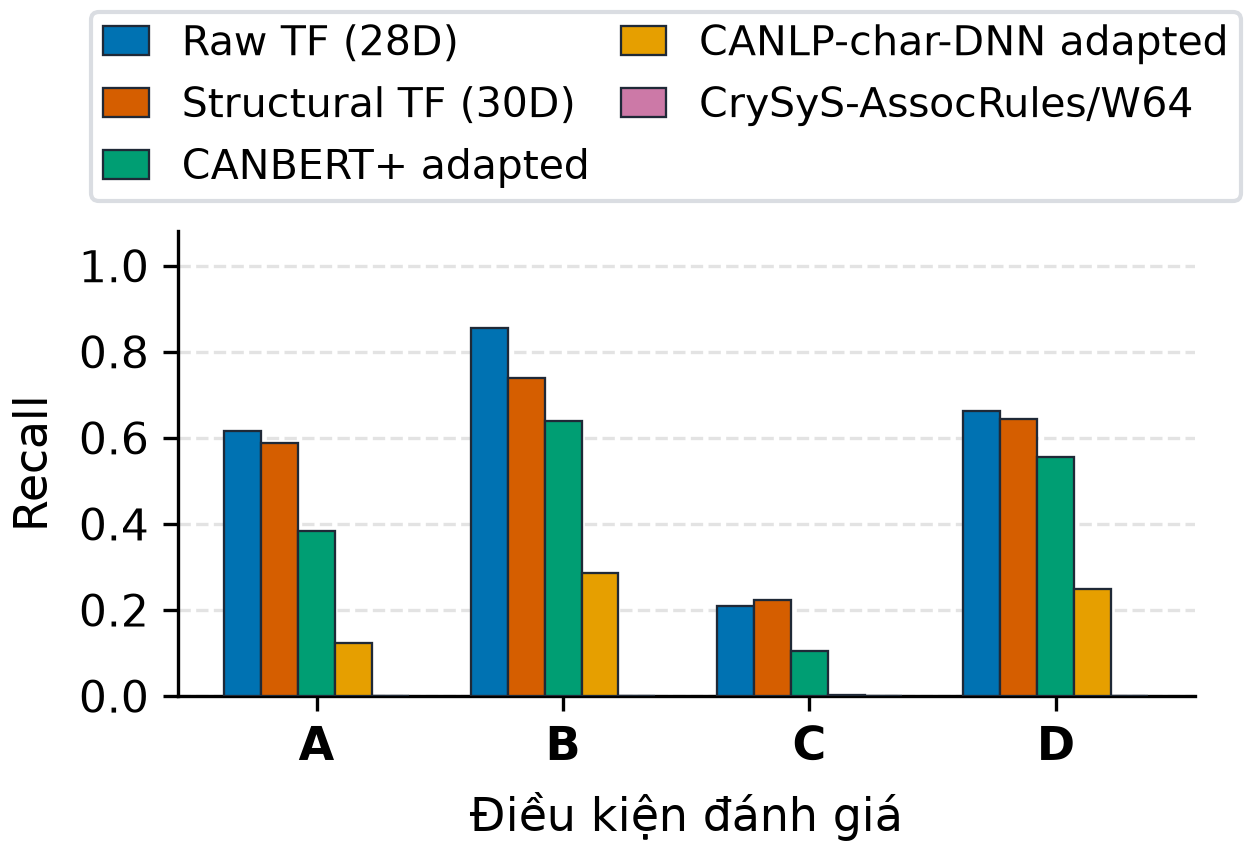
\includegraphics[width=\linewidth]{figs/comparison_v1_vi_Recall.png}
  \caption{Recall}\label{subfig:comp-recall}
\end{subfigure}\hfill
\begin{subfigure}[b]{0.45\textwidth}
  \centering
  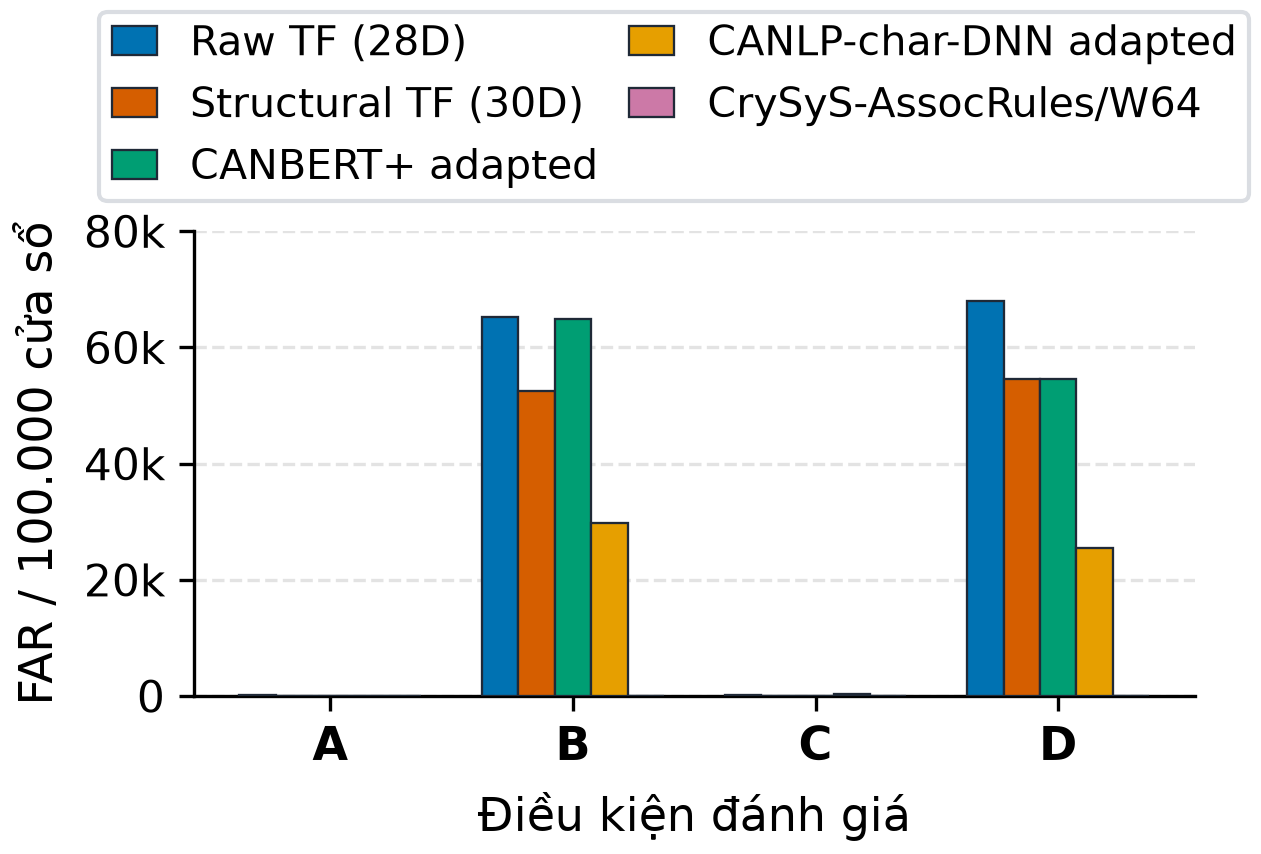
\includegraphics[width=\linewidth]{figs/comparison_v1_vi_FAR_per_100k.png}
  \caption{FAR trên $100.000$ cửa sổ}\label{subfig:comp-far}
\end{subfigure}
\vskip 2pt
\begin{subfigure}[b]{0.45\textwidth}
  \centering
  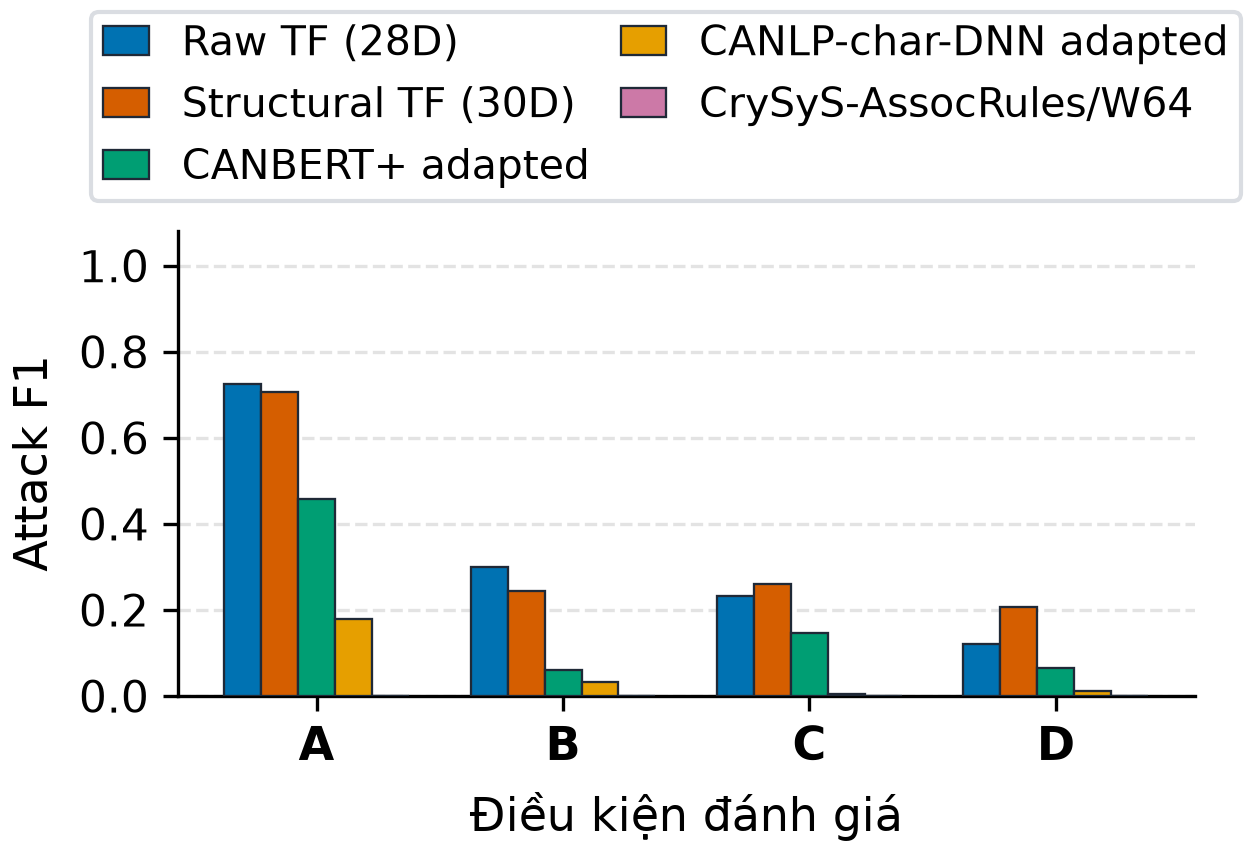
\includegraphics[width=\linewidth]{figs/comparison_v1_vi_Attack_F1.png}
  \caption{Attack F1}\label{subfig:comp-f1}
\end{subfigure}\hfill
\begin{subfigure}[b]{0.45\textwidth}
  \centering
  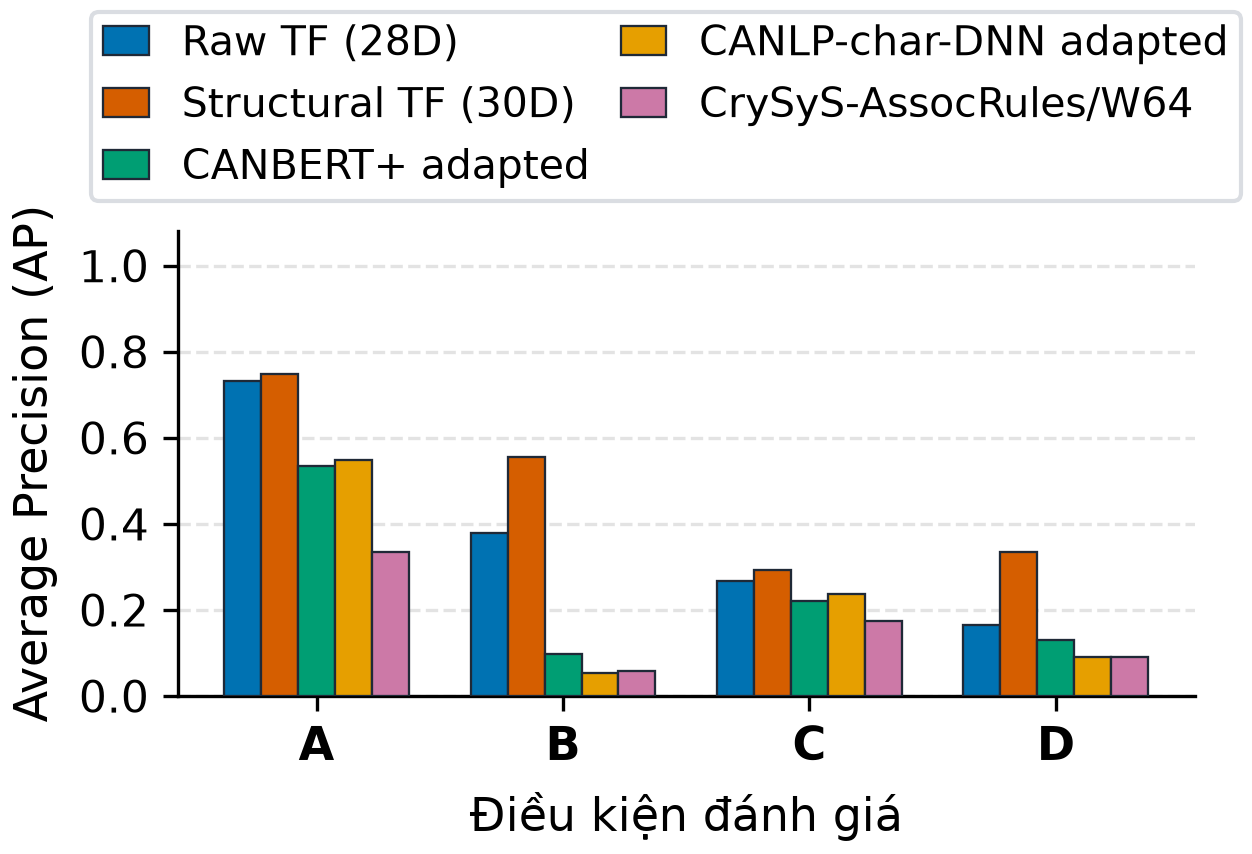
\includegraphics[width=\linewidth]{figs/comparison_v1_vi_AP.png}
  \caption{Average Precision (AP)}\label{subfig:comp-ap}
\end{subfigure}
\caption[Kết quả đối sánh năm phương pháp ở cửa sổ $W=64$ qua bốn điều kiện A--D]{Kết quả đối sánh năm phương pháp ở cửa sổ $W=64$ qua bốn điều kiện A--D dưới ngưỡng nguồn (trọng số bốn tập ngang nhau).}\label{fig:comparison-four-metrics}
\end{figure}

Từ Bảng~\ref{tab:comparison-main}, Hình~\ref{fig:comparison-four-metrics} và đối chứng chênh lệch ghép cặp tại Bảng~\ref{tab:comparison-paired} (Phụ lục~\ref{app:sensitivity}), ở điều kiện chuyển xe B, Structural đạt recall thấp hơn Raw $-11{,}59$ điểm phần trăm ($0{,}7383$ so với $0{,}8541$) với tỷ lệ báo động giả còn rất cao ($\text{FAR} = 52{,}46\%$, tương đương $52.461{,}46/100\text{k}$ cửa sổ); tuy nhiên về chất lượng xếp hạng độc lập ngưỡng, AP tăng $+0{,}1774$ ghép cặp ($+0{,}1773$ chênh lệch trung bình, từ $0{,}3781$ lên $0{,}5554$, vượt xa CANBERT+ $0{,}0970$ với $\Delta\text{AP} = +0{,}4584$ và CANLP $0{,}0542$ với $\Delta\text{AP} = +0{,}5012$). Ở Điều kiện D (chuyển cả xe và tấn công), AP tăng từ $0{,}1648$ lên $0{,}3357$ ($\Delta\text{AP} = +0{,}1709$ ghép cặp so với Raw, $\Delta\text{AP} = +0{,}2046$ so với CANBERT+; FAR còn $54{,}64\%$). Khi khử lặp trọng số xe đích Subaru Forester (áp dụng trọng số $1/3, 1/6, 1/6, 1/3$), xu hướng hoàn toàn nhất quán: ở B, Structural đạt recall $0{,}6610$, FAR $41{,}26\%$, F1 $0{,}2891$, AP $0{,}5510$ (so với Raw $0{,}8722$, $60{,}23\%$, $0{,}3629$, $0{,}4281$); ở D đạt AP $0{,}3404$ và FAR $43{,}60\%$ (so với Raw $0{,}1799$ và $63{,}69\%$). Do đó giả thuyết ban đầu về việc biểu diễn cấu trúc tự động tăng recall tại ngưỡng tĩnh đóng băng nguồn không được ủng hộ bởi thực nghiệm.

Phân rã chi tiết theo từng tập và hạt giống ngẫu nhiên (Bảng~\ref{tab:comparison-sets}, khoảng bootstrap ở Bảng~\ref{tab:comparison-ci}, và phân rã AP chi tiết tại Bảng~\ref{tab:per-set-ap-breakdown}, Phụ lục~\ref{app:reproducibility}) làm rõ bức tranh chuyển giao: ba hạt giống ngẫu nhiên đại diện cho phương sai tối ưu hóa mô hình chứ không tương đương ba xe độc lập, và 4 tập đối chuẩn can-train-and-test chỉ bao gồm 3 xe đích vật lý riêng biệt (Chevrolet Silverado ở Set 1, Subaru Forester ở Set 2--3, và Chevrolet Traverse ở Set 4). Tại Điều kiện B, mức cải thiện AP của Structural so với Raw ($\Delta\text{AP}$) có sự phân hóa rõ nét theo mức độ tương đồng kiến trúc bus: ở Set~1 (nội bộ dòng Chevrolet), Raw tận dụng được ID trùng khớp và đạt AP cao hơn Structural ($\Delta\text{AP} = -0{,}0983 \pm 0{,}1408$); ngược lại trên các cặp xe khác hãng, Structural thể hiện ưu thế vượt trội ($\Delta\text{AP} = +0{,}2244 \pm 0{,}2325$ ở Set~2; $+0{,}4566 \pm 0{,}0778$ ở Set~3; $+0{,}1267 \pm 0{,}0071$ ở Set~4), đưa mức tăng AP trung bình toàn diện đạt $+0{,}1774$. Tại Điều kiện D, Structural cũng thắng áp đảo ở 3/4 tập (cao nhất $+0{,}3287$ ở Set 3 và $+0{,}3158$ ở Set 4; trung bình $+0{,}1709$), chỉ giảm nhẹ $-0{,}0360$ ở Set 1. Về ngưỡng vận hành tại Set~1, Structural giữ FAR rất thấp ($32{,}14/100\text{k}$ so với Raw $168{,}99/100\text{k}$), nhưng ở Set 2--4 sự trôi dạt nền phân phối điểm số khiến FAR bùng nổ lên $37{,}7\%\text{--}100\%$, dẫn đến hàng chục nghìn cảnh báo giả mỗi giờ ở tốc độ bus $1.000\text{--}2.000$ khung/giây và làm tê liệt khả năng vận hành khả thi. Hiện tượng này khẳng định phân tách độc lập giữa chất lượng xếp hạng (AP) và hiệu năng vận hành tại ngưỡng nguồn, đồng thời xác lập việc hiệu chuẩn ngưỡng là điều kiện bắt buộc đối với IDS nội xe~\cite{axelsson2000base,sommer2010outside,saito2015pr,lampe2024curated}.

\noindent\textbf{Chuyển tiếp sang động học thời gian và tính đơn điệu timestamp:} Hiện tượng sụp đổ ngưỡng vận hành và bùng nổ FAR ở Điều kiện B quan sát thấy ở trên phần lớn bắt nguồn từ việc buộc phải loại bỏ hoàn toàn các đặc trưng thời gian ($\Delta t$) nhằm đảm bảo an toàn trước 100 tệp CTT bị lỗi đồng hồ đi lùi. Tác động có kiểm soát của động học thời gian ($\Delta t$ và $\Delta t_{\text{ID}}$) trên 136 tệp có dấu thời gian đơn điệu nghiêm ngặt được phân tích chi tiết tại Mục~\ref{subsec:timed-vs-content} (Bảng~\ref{tab:monotonic-timed-vs-content}) ngay dưới đây.

\subsubsection{Điểm vận hành suy biến của AssocRules}\label{subsec:assoc-degenerate}
Cả 12 ngưỡng nguồn của \code{CrySyS-AssocRules/W64} đều suy biến tại $1 + \varepsilon_{\text{mach}} > 1{,}0$ (giá trị máy $1{,}0000000000000002$, dự đoán toàn bộ là benign: $R=0, \text{FAR}=0$) do không có bất kỳ ngưỡng khả dĩ nào thỏa mãn ngân sách $\text{FAR} \le 100/100\text{k}$; tại điểm $1{,}0$, FAR validation nguồn đã nằm trong khoảng $348{,}58\text{--}4696{,}34/100\text{k}$ (vượt ngân sách; chi tiết phân phối điểm số bất thường tại Bảng~\ref{tab:assoc-scores}, Mục~\ref{sec:app-assoc-scores}). Ngay cả khi huấn luyện lại trên 5.000 cửa sổ lành liên tục của Set~1, tỷ lệ cửa sổ validation đạt điểm $1{,}0$ vẫn là $0{,}44\%$ ($440/100\text{k}$). Việc thuật toán chọn ngưỡng tự động đẩy ngưỡng lên trên điểm số cực đại đã biến toàn bộ dự đoán thành lớp lành tính, tạo ra một điểm vận hành suy biến cần được ghi nhận minh bạch thay vì hiểu lầm là mô hình không có báo động giả. Ở chỉ số AP độc lập ngưỡng, AssocRules chỉ đạt $0{,}0591$ (B) và $0{,}0912$ (D), và trên xe lạ 100\% cửa sổ đích nhận điểm $1{,}0$ (\code{frac\_score\_1} $=1{,}0000$).

\noindent\textbf{Tác động của quy tắc gộp điểm khung tin và sai lệch quy nạp (Window Aggregation Bias):} Các mô hình đối thủ \code{CANLP} và \code{CANBERT+} là mô hình phân loại cấp khung tin (frame-level), và điểm số cửa sổ được tính qua phép gộp cực đại: $s_{\text{window}} = \max_{j=1}^{64} s_j$. Phép toán $\max$ này khuếch đại xác suất báo động giả của cả cửa sổ theo cấp số nhân: nếu xác suất báo động giả ở mỗi khung tin là $\epsilon$, thì xác suất ít nhất một khung tin bị báo động nhầm trong cửa sổ 64 khung tin là $\text{FAR}_{\text{window}} = 1 - (1 - \epsilon)^{64} \approx 64\epsilon$. Điều này đặt các baseline frame-level vào thế bất lợi thống kê rất lớn dưới cùng một ngưỡng ngân sách FAR cứng so với cơ chế Global Average Pooling của Transformer. Đánh giá lại chuỗi điểm khung đã lưu với quy tắc \code{max}, \code{top8\_mean} và \code{mean} (Mục~\ref{subsec:baseline-pooling-ablation}, Bảng~\ref{tab:baseline-pooling-ablation}, Phụ lục~\ref{app:sensitivity}) cho thấy quy tắc \code{mean} khắc phục ép ngưỡng ở A cho \code{CANLP} (Recall $0{,}1228 \to 0{,}4125$), nhưng AP đa xe ở B của \code{CANBERT+} ($0{,}1636$) và \code{CANLP} ($0{,}1982$) vẫn thua xa \code{Structural} ($0{,}5554$).

\subsubsection{Phân bố số lượng cửa sổ dương/âm từng tệp ở Điều kiện B và D}\label{subsec:bd-per-file-counts}
Bảng~\ref{tab:bd-per-file-counts} tại Mục~\ref{sec:app-bd-per-file-counts} (Phụ lục~\ref{app:reproducibility}) thống kê phân bố trên toàn bộ 88 tệp B và D nhằm diễn giải đúng Bảng~\ref{tab:comparison-main}--\ref{tab:benign-calibration-summary}: tỷ lệ dương từng tệp biến thiên hơn ba bậc độ lớn, từ $0{,}00\%$ (bản ghi \textit{force-neutral} thuộc Tập~4, Điều kiện~D, 0/7.096) và $0{,}03\%$ (bản ghi \textit{speed} thuộc Tập~4, Điều kiện~B, 14/40.932) tới $97{,}81\%$ (bản ghi \textit{interval} thuộc Tập~4, Điều kiện~B, 9.692/9.909) và $96{,}92\%\text{--}97{,}22\%$ ở Tập~3, Điều kiện~D.

\noindent\textbf{Trả lời trực diện RQ1:} Biểu diễn cấu trúc giúp cải thiện vượt bậc khả năng phân tách và chất lượng xếp hạng độc lập ngưỡng trên phương tiện chưa từng thấy ($\Delta\text{AP} = +0{,}1774$ ở B và $+0{,}1709$ ở D), song việc dịch chuyển phân phối nền lành tính vẫn khiến ngưỡng quyết định đóng băng từ nguồn bị trôi dạt nghiêm trọng ($\text{FAR} \approx 52{,}46\%\text{--}54{,}64\%$), khẳng định việc chỉ loại bỏ định danh thô là chưa đủ để giải quyết bài toán zero-shot tại ngưỡng nguồn mà bắt buộc phải có cơ chế thích ứng hoặc hiệu chuẩn vận hành.

\subsection{Tác động của động học thời gian: Đối chứng Timed 32D và Content 30D trên 136 tệp đơn điệu}\label{subsec:timed-vs-content}
Một phát hiện mang tính then chốt của luận văn là: hiện tượng sụp đổ điểm vận hành của bộ phân loại nguồn ở Điều kiện B một phần lớn là hệ quả phụ của quyết định loại bỏ triệt để biến thời gian $\Delta t$ nhằm bảo đảm tính toàn vẹn trước các tệp nhật ký bị lỗi đồng hồ ghi lùi. Để định lượng chính xác tác động độc lập của động học thời gian, nghiên cứu thực hiện đối chứng có kiểm soát giữa nhánh \code{Content} (28D/30D) và \code{Timed} (29D/32D) trên tập con 136/236 tệp CTT có dấu thời gian đơn điệu nghiêm ngặt (không có bất kỳ vi phạm thời gian nào). Kết quả đối chứng trực tiếp được trình bày tại Bảng~\ref{tab:monotonic-timed-vs-content}.

{\footnotesize\setlength{\tabcolsep}{3.5pt}\renewcommand{\arraystretch}{0.88}
\begin{longtable}{P{2.8cm}P{1.7cm}P{0.7cm}P{2.1cm}P{1.5cm}P{1.4cm}P{2.1cm}}
\caption[Đối chứng nhánh Content (28D/30D) và Timed (29D/32D) trên 136 tệp đơn điệu]{Đối chứng trực tiếp hiệu năng giữa nhánh \code{Content} (28D/30D) và \code{Timed} (29D/32D) trên tập con 136/236 tệp CTT có dấu thời gian đơn điệu nghiêm ngặt (trung bình bốn tập và ba hạt giống; giá trị trong ngoặc là trung bình ba xe đích khử lặp)}\label{tab:monotonic-timed-vs-content}\\\toprule
Nhánh / Mô hình & Ngưỡng & ĐK & Recall (3-xe) & FAR (\%) & F1 & AP (3-xe)\\\midrule
\endfirsthead
\caption[]{(tiếp theo)}\\\toprule
Nhánh / Mô hình & Ngưỡng & ĐK & Recall (3-xe) & FAR (\%) & F1 & AP (3-xe)\\\midrule
\endhead
Content Raw (28D) & Nguồn & A & 0,7410 & 0,065\% & 0,8390 & 0,8923\\
Timed Raw (29D) & Nguồn & A & 0,6371 & 0,108\% & 0,7467 & 0,8399\\
Content Structural (30D) & Nguồn & A & 0,6100 & 0,088\% & 0,7217 & 0,8182\\
\textbf{Timed Structural (32D)} & Nguồn & A & \textbf{0,8405} & 0,085\% & \textbf{0,8996} & \textbf{0,9638}\\
\midrule
Content Raw & Nguồn & B & 0,9206 (0,8973) & 76,38\% & 0,2624 & 0,5377 (0,6070)\\
Timed Raw & Nguồn & B & 0,8249 (0,8086) & 65,88\% & 0,2560 & 0,5788 (0,6501)\\
Content Structural & Nguồn & B & 0,6479 (0,5808) & 41,16\% & 0,2360 & 0,5786 (0,6123)\\
\textbf{Timed Structural} & Nguồn & B & 0,8123 (\textbf{0,8711}) & \textbf{2,46\%} & \textbf{0,8274} & \textbf{0,9359} (\textbf{0,9508})\\
Content Raw & Nguồn & C & 0,1592 & 0,081\% & 0,1933 & 0,3077\\
Timed Raw & Nguồn & C & 0,1808 & 0,065\% & 0,2295 & 0,3561\\
Content Structural & Nguồn & C & 0,1715 & 0,078\% & 0,2164 & 0,3699\\
\textbf{Timed Structural} & Nguồn & C & \textbf{0,5015} & \textbf{0,065\%} & \textbf{0,5212} & \textbf{0,7537}\\
\midrule
Content Raw & $K=500$, 1,0\% & B & 0,4540 (0,5190) & 0,67\% & 0,5192 & 0,5424 (0,6119)\\
Timed Raw & $K=500$, 1,0\% & B & 0,4857 (0,5442) & 0,70\% & 0,5585 & 0,5850 (0,6572)\\
Content Structural & $K=500$, 1,0\% & B & 0,4264 (0,4689) & 2,24\% & 0,5225 & 0,5857 (0,6185)\\
\textbf{Timed Structural} & $K=500$, 1,0\% & B & \textbf{0,7460} (\textbf{0,8035}) & \textbf{0,63\%} & \textbf{0,8295} & \textbf{0,9451} (\textbf{0,9575})\\
Content Raw & $K=500$, 1,0\% & D & 0,1009 (0,1308) & 1,20\% & 0,1368 & 0,1990 (0,2287)\\
Timed Raw & $K=500$, 1,0\% & D & 0,1192 (0,1544) & 0,93\% & 0,1635 & 0,2325 (0,2684)\\
Content Structural & $K=500$, 1,0\% & D & 0,2537 (0,3065) & 0,62\% & 0,3213 & 0,3904 (0,4190)\\
\textbf{Timed Structural} & $K=500$, 1,0\% & D & \textbf{0,4036} (\textbf{0,4341}) & \textbf{0,28\%} & \textbf{0,4742} & \textbf{0,7219} (\textbf{0,6736})\\
\bottomrule
\end{longtable}}

Từ Bảng~\ref{tab:monotonic-timed-vs-content}, khóa luận xác lập hai kết luận phương pháp luận cốt lõi:
\begin{enumerate}
    \item \textbf{Hai chế độ vận hành độc lập của hệ thống phát hiện xâm nhập:}
    \begin{itemize}
        \item \textit{Chế độ Bus đồng hồ chuẩn (Clean-Clock Bus):} Khi dấu thời gian vật lý đạt độ tin cậy đơn điệu, sự kết hợp giữa cú pháp khung tin và động học thời gian ($\Delta t, \Delta t_{\text{ID}}$) trong mô hình \textbf{Timed Structural (32D)} cải thiện đáng kể AP và giảm mạnh FAR trên tập con 136 tệp đơn điệu so với Content 30D: ở Điều kiện B, FAR giảm từ $41{,}16\%$ xuống $\mathbf{2{,}46\%}$, Recall đạt $\mathbf{81{,}23\%}$ ($87{,}11\%$ khử lặp 3 xe), F1 đạt $0{,}8274$ và AP vọt lên $\mathbf{0{,}9359}$ ($0{,}9508$ khử lặp). Tuy nhiên, mức FAR $2{,}46\%$ vẫn cao gấp 24,6 lần ngân sách nguồn $0{,}1\%$, cho thấy bài toán chuyển giao zero-shot thực tế chưa được giải quyết trọn vẹn mà vẫn đòi hỏi hiệu chuẩn ngưỡng vận hành dưới các điều kiện thời gian ngặt nghèo. Trái lại, \code{Timed Raw (29D)} chỉ tăng nhẹ AP lên $0{,}5788$ nhưng FAR vẫn vỡ ở mức $65{,}88\%$, chứng minh rằng chỉ riêng thời gian không đủ mà bắt buộc phải có cú pháp cấu trúc ID-invariant.
        \item \textit{Chế độ Log thiếu/nhiễu thời gian (Timing-Degraded / Log-Only Bus):} Khi dấu thời gian bị mất, trôi dạt hoặc chịu lỗi đảo ngược sub-millisecond như trên 100 tệp CTT, mô hình \textbf{Content Structural (30D)} đóng vai trò cận dưới bảo thủ an toàn. Trong chế độ này, sự sụp đổ ngưỡng nguồn được cứu vãn triệt để thông qua cơ chế hiệu chuẩn nền lành tính gộp đa tệp (Giai đoạn 2), cải thiện đáng kể kiểm soát FAR thực nghiệm trung bình về mức $\le 1{,}08\%$ trên các tập đối chuẩn.
    \end{itemize}
    \item \textbf{Hiệu năng sau hiệu chuẩn nền lành tính:} Khi kết hợp hiệu chuẩn nền lành tính ($K=500, \alpha=1{,}0\%$), \code{Timed Structural} đạt $\text{AP}_B=0{,}9451$ (Recall $74{,}60\%$, FAR $0{,}63\%$) và $\text{AP}_D=0{,}7219$ (Recall $40{,}36\%$, FAR $0{,}28\%$), vượt trội áp đảo toàn bộ các biến thể content-only.
\end{enumerate}

\subsection{Phân tích vai trò thành phần biểu diễn và độ nhạy kích thước cửa sổ (RQ2)}\label{sec:completion}
Bảng~\ref{tab:extension-w64} trình bày kết quả phân tích cắt bỏ trên 10 biến thể biểu diễn tại kích thước cửa sổ chuẩn $W=64$, trong khi các đánh giá độ nhạy tương ứng tại $W \in \{32, 128\}$ được tổng hợp chi tiết tại Bảng~\ref{tab:extension-w32} (Phụ lục~\ref{app:sensitivity}).

\Needspace{6\baselineskip}
{\footnotesize\renewcommand{\arraystretch}{0.84}
\begin{longtable}{P{1.1cm}P{4.9cm}P{1.6cm}P{2.2cm}P{1.6cm}P{1.6cm}}
\caption[Kết quả cắt bỏ thành phần biểu diễn trên 10 biến thể ở $W=64$]{Kết quả đối chứng cắt bỏ thành phần biểu diễn trên 10 biến thể ở kích thước cửa sổ $W=64$ (trọng số bốn tập ngang nhau; FAR tính trên $100.000$ cửa sổ lành)}\label{tab:extension-w64}\\\toprule
ĐK & Phương pháp & Recall & FAR & F1 & AP\\\midrule
\endfirsthead\caption[]{(tiếp theo)}\\\toprule
ĐK & Phương pháp & Recall & FAR & F1 & AP\\\midrule
\endhead
A & Chỉ ID & 0,7655 & 90,54 & 0,8439 & 0,8492\\
B & Chỉ ID & 0,8622 & 68896,67 & 0,2573 & 0,3379\\
C & Chỉ ID & 0,1978 & 93,00 & 0,2358 & 0,2736\\
D & Chỉ ID & 0,6822 & 67788,42 & 0,1857 & 0,1914\\
A & Raw & 0,6167 & 115,77 & 0,7258 & 0,7312\\
B & Raw & 0,8541 & 65301,41 & 0,3000 & 0,3781\\
C & Raw & 0,2101 & 91,92 & 0,2314 & 0,2661\\
D & Raw & 0,6614 & 67982,89 & 0,1213 & 0,1648\\
A & Raw bỏ ID & 0,2533 & 100,13 & 0,3668 & 0,4139\\
B & Raw bỏ ID & 0,6794 & 66658,13 & 0,0875 & 0,2200\\
C & Raw bỏ ID & 0,0906 & 62,70 & 0,1466 & 0,2222\\
D & Raw bỏ ID & 0,6871 & 66679,05 & 0,1677 & 0,2175\\
A & Raw cộng cấu trúc & 0,6515 & 84,74 & 0,7380 & 0,7428\\
B & Raw cộng cấu trúc & 0,7604 & 53227,73 & 0,3179 & 0,4842\\
C & Raw cộng cấu trúc & 0,1950 & 91,68 & 0,2296 & 0,2703\\
D & Raw cộng cấu trúc & 0,5783 & 52902,70 & 0,1567 & 0,2976\\
A & Structural & 0,5886 & 81,67 & 0,7072 & 0,7483\\
B & Structural & 0,7383 & 52461,46 & 0,2435 & 0,5554\\
C & Structural & 0,2230 & 75,82 & 0,2600 & 0,2928\\
D & Structural & 0,6445 & 54643,37 & 0,2069 & 0,3357\\
A & Structural bỏ delta & 0,4910 & 89,84 & 0,6050 & 0,6789\\
B & Structural bỏ delta & 0,8306 & 58636,28 & 0,2861 & 0,4927\\
C & Structural bỏ delta & 0,2006 & 73,86 & 0,2363 & 0,2720\\
D & Structural bỏ delta & 0,6795 & 60669,40 & 0,1815 & 0,2745\\
A & Structural bỏ thống kê cục bộ & 0,4851 & 100,21 & 0,6147 & 0,6346\\
B & Structural bỏ thống kê cục bộ & 0,6870 & 65298,51 & 0,0948 & 0,2894\\
C & Structural bỏ thống kê cục bộ & 0,1955 & 99,41 & 0,2412 & 0,2795\\
D & Structural bỏ thống kê cục bộ & 0,6925 & 66400,30 & 0,1626 & 0,3053\\
A & Structural bỏ payload tuyệt đối & 0,6243 & 87,77 & 0,7317 & 0,7644\\
B & Structural bỏ payload tuyệt đối & 0,9243 & 66779,19 & 0,3160 & 0,4453\\
C & Structural bỏ payload tuyệt đối & 0,3328 & 101,16 & 0,4076 & 0,4730\\
D & Structural bỏ payload tuyệt đối & 0,7202 & 67775,85 & 0,2024 & 0,3138\\
A & Structural bỏ hạng/W & 0,5308 & 79,90 & 0,6507 & 0,6837\\
B & Structural bỏ hạng/W & 0,7998 & 59718,63 & 0,2425 & 0,5266\\
C & Structural bỏ hạng/W & 0,2650 & 75,73 & 0,3247 & 0,3420\\
D & Structural bỏ hạng/W & 0,6881 & 62056,45 & 0,1830 & 0,3446\\
A & Structural bỏ chuyển tiếp & 0,5567 & 66,87 & 0,6784 & 0,7044\\
B & Structural bỏ chuyển tiếp & 0,7137 & 53236,21 & 0,2220 & 0,5556\\
C & Structural bỏ chuyển tiếp & 0,2419 & 76,67 & 0,2896 & 0,3210\\
D & Structural bỏ chuyển tiếp & 0,6665 & 55254,24 & 0,2049 & 0,3679\\
\bottomrule\end{longtable}}



Các phép cắt bỏ ở Bảng~\ref{tab:extension-w64} cho thấy: (1) Loại bỏ ID đơn thuần khỏi Raw làm recall B giảm từ $0{,}8541$ xuống $0{,}6794$ và AP giảm từ $0{,}3781$ xuống $0{,}2200$; (2) Nhóm thống kê cục bộ đóng vai trò sống còn đối với AP và kiểm soát FAR (cắt bỏ làm AP B tụt từ $0{,}5554$ xuống $0{,}2894$ và FAR tăng lên $65.298{,}51/100\text{k}$); (3) Bỏ delta làm AP B giảm còn $0{,}4927$, còn bỏ chuyển tiếp giữ AP B xấp xỉ $0{,}5556$ và tăng nhẹ AP D ($0{,}3679$); (4) Đáng chú ý, bỏ payload tuyệt đối làm tăng FAR ở B ($66.779{,}19/100\text{k}$, AP giảm còn $0{,}4453$) nhưng lại nâng mạnh hiệu năng tấn công mới ở Điều kiện C (F1 $0{,}4076$, AP $0{,}4730$ so với Raw $0{,}2661$ và Structural $0{,}2928$), chứng tỏ giá trị byte payload tuyệt đối dễ làm mô hình quá khớp vào chữ ký tấn công nguồn. Việc giữ lại cả hai chiều 28 ($\operatorname{rank}_0/W$) và 29 (chuyển tiếp ID) trong biểu diễn chuẩn 30D xuất phát từ mục tiêu thiết kế toàn diện được xác định trước (\textit{a priori}): chiều 28 cung cấp thang đo mật độ cố định chuẩn hóa theo cửa sổ $W$ độc lập với biến động số lượng ID phân biệt $U_k$ (hỗ trợ độ nhạy khi $W$ thay đổi ở Bảng~\ref{tab:extension-w32}, cải thiện AP ở Điều kiện A và B, đồng thời kìm hãm FAR ở Điều kiện B và D); trong khi chiều 29 mã hóa động học cặp chuyển tiếp liền kề giúp nâng cao rõ rệt hiệu năng trong miền tại Điều kiện A ($+3{,}19$ điểm phần trăm Recall, $+4{,}39$ điểm phần trăm AP) cũng như Điều kiện B ($+2{,}46$ điểm phần trăm Recall, $+2{,}15$ điểm phần trăm F1 và giảm nhẹ FAR). Dù việc lược bỏ riêng chiều 28 hoặc chiều 29 mang lại lợi thế cục bộ cho Điều kiện D ($0{,}3446$ và $0{,}3679$ AP so với $0{,}3357$), không gian 30D nguyên bản được ưu tiên nhằm tối đa hóa độ cân bằng đa điều kiện; việc tỉa gọn các chiều này mở ra một biến thể thu gọn đầy tiềm năng cho kịch bản tấn công chưa từng thấy. Ở Bảng~\ref{tab:extension-w32} (Phụ lục~\ref{app:sensitivity}), chênh lệch recall Structural trừ Raw ở B đổi dấu theo kích thước cửa sổ ($+0{,}69$ điểm phần trăm ở $W=32$, $-11{,}59$ điểm phần trăm ở $W=64$, $+1{,}28$ điểm phần trăm ở $W=128$) với FAR đều trên $53\%$.

\noindent\textbf{Độ nhạy đẳng lượng khung tin và phương sai lấy mẫu reservoir:} Dưới kiểm chứng đẳng lượng $64.000$ khung/tệp/lớp qua $W \in \{32, 64, 128\}$ và qua ba hạt giống lấy mẫu reservoir độc lập (chi tiết tại Mục~\ref{subsec:frame-equated-w-and-reservoir}, Bảng~\ref{tab:frame-equated-w} và Bảng~\ref{tab:reservoir-variance}, Phụ lục~\ref{app:sensitivity}), \code{Structural} tiếp tục vượt trội \code{Raw} về AP trên mọi kích thước cửa sổ và duy trì ổn định điểm tối ưu tại $W=64$ ($\text{AP}_B=0{,}5607$ sau hiệu chuẩn so với $0{,}4304$ ở $W=32$ và $0{,}4903$ ở $W=128$).

\noindent\textbf{Trả lời trực diện RQ2:} Nhóm đặc trưng thống kê cục bộ và biến thiên tải trọng là hai trụ cột quyết định giúp duy trì chất lượng phân tách và kiểm soát FAR khi chuyển giao xe, trong khi cửa sổ $W=64$ xác lập điểm cân bằng tối ưu giữa ngữ cảnh chuỗi và độ trễ phát hiện so với các cửa sổ $W=32$ và $W=128$.

\subsection{Đánh giá mức độ độc lập xe và phân tách tấn công qua thăm dò tuyến tính (RQ3)}\label{sec:eval-probes}
Bảng~\ref{tab:extension-probes} tổng hợp kết quả Linear Probe trên 12 cặp bộ mã hóa đóng băng (chia tách theo vòng ghi, cân bằng ô xe $\times$ nhãn; kết quả tổng hợp đầy đủ trên toàn bộ 10 biến thể biểu diễn được lưu trữ tại Phụ lục~\ref{sec:app-96ckpt-probes}). Trong khi khả năng giải mã nhãn tấn công tăng $+12{,}50$ điểm phần trăm từ $0{,}6419$ (Raw) lên $0{,}7669$ (Structural), độ chính xác giải mã xe chỉ giảm $4{,}37$ điểm phần trăm từ $0{,}9925$ xuống $0{,}9488$ (còn cách xa mức ngẫu nhiên $0{,}2500$; các đối chứng hằng/ngẫu nhiên/hoán vị đều quanh $0{,}25$ và $0{,}50$).

{\renewcommand{\arraystretch}{0.85}
\begin{table}[htbp]\centering\footnotesize
\caption[Kết quả thăm dò tuyến tính và đối chứng Hewitt--Liang trên bộ mã hóa đóng băng]{Kết quả thăm dò tuyến tính và các đối chứng Hewitt--Liang trên biểu diễn ẩn của hai bộ mã hóa Raw và Structural (Balanced Accuracy trung bình qua bốn tập và ba hạt giống)}\label{tab:extension-probes}
\begin{tabular}{P{3.3cm}P{1.6cm}P{4.7cm}P{3.1cm}}
\toprule
Biểu diễn & Nhãn & Đối chứng & Balanced accuracy\\\midrule
raw & attack & constant & 0,5000\\
raw & attack & learned & 0,6419\\
raw & attack & permuted train labels & 0,5106\\
raw & attack & random embedding & 0,5026\\
raw & vehicle & constant & 0,2500\\
raw & vehicle & learned & 0,9925\\
raw & vehicle & permuted train labels & 0,2444\\
raw & vehicle & random embedding & 0,2496\\
structural & attack & constant & 0,5000\\
structural & attack & learned & 0,7669\\
structural & attack & permuted train labels & 0,4958\\
structural & attack & random embedding & 0,5026\\
structural & vehicle & constant & 0,2500\\
structural & vehicle & learned & 0,9488\\
structural & vehicle & permuted train labels & 0,2287\\
structural & vehicle & random embedding & 0,2496\\
\bottomrule\end{tabular}
\end{table}}

\subsubsection{Chẩn đoán nguồn gốc rò rỉ thông tin xe và đan xen đặc trưng}
Để giải thích nguyên nhân rò rỉ xấp xỉ $95\%$ khi đã loại bỏ hoàn toàn 11-bit CAN-ID, Bảng~\ref{tab:input-feature-probes} cô lập từng nhóm đặc trưng đầu vào trên $8.440$ cửa sổ cân bằng ($3.800$ train / $4.640$ test giữ ngoài theo vòng ghi; đối chiếu độ nhạy $C$ ở Mục~\ref{sec:probe-audit} và Bảng~\ref{tab:probe-c-scaling}, Phụ lục~\ref{app:sensitivity}).

{\renewcommand{\arraystretch}{0.85}
\begin{table}[htbp]\centering\footnotesize
\caption{Khả năng giải mã tuyến tính nhãn xe và nhãn tấn công từ từng nhóm đặc trưng đầu vào cô lập ($W=64$)}\label{tab:input-feature-probes}
\begin{tabular}{P{6.2cm}C{1.6cm}C{2.1cm}C{1.6cm}C{2.1cm}}
\toprule
Nhóm đặc trưng đầu vào & Số chiều / khung & Tổng chiều ($W=64$) & Probe xe & Probe tấn công\\\midrule
Tất cả 30 đặc trưng (Structural) & 30 & 1920 & 0,9804 & 0,7487\\
DLC, mặt nạ hợp lệ và cờ $h_i$ (\texttt{dlc\_and\_masks}) & 10 & 640 & \textbf{0,9670} & 0,6289\\
\quad -- Bóc tách riêng DLC và 8 mặt nạ (chỉ 9 chiều) & 9 & 576 & 0,9642 & 0,5946\\
\quad -- Bóc tách riêng cờ lịch sử $h_i$ (chỉ số 25) & 1 & 64 & 0,2746 & 0,5662\\
Chỉ thống kê cục bộ (\texttt{local\_stats}) & 3 & 192 & \textbf{0,7565} & \textbf{0,7269}\\
Chỉ Payload thô (\texttt{payload}) & 8 & 512 & 0,7621 & 0,5601\\
Chỉ Biến thiên payload ($\Delta\text{payload}$) & 8 & 512 & 0,6498 & 0,6420\\
Chỉ Chuyển tiếp ID (\texttt{transition}) & 1 & 64 & 0,4627 & 0,5013\\
\midrule
Loại bỏ Payload thô (\texttt{no\_payload}) & 22 & 1408 & 0,9565 & 0,7578\\
Loại bỏ Biến thiên payload (\texttt{no\_delta}) & 22 & 1408 & 0,9884 & 0,7252\\
Loại bỏ Thống kê cục bộ (\texttt{no\_local\_stats}) & 27 & 1728 & 0,9541 & 0,6319\\
Loại bỏ Chuyển tiếp ID (\texttt{no\_transition}) & 29 & 1856 & 0,9778 & 0,7241\\
\midrule
\multicolumn{5}{P{13.5cm}}{\footnotesize \textit{Ghi chú:} Hàng \texttt{no\_delta} ở bảng này có 22 chiều do chỉ loại bỏ 8 chiều $\Delta\text{payload}$ để cô lập ảnh hưởng của biến thiên byte thô (giữ lại 1 chiều cờ $h_i$ thuộc nhóm \texttt{dlc\_and\_masks}); khác với biến thể cắt bỏ mô hình \texttt{structural\_no\_delta} 21 chiều ở Mục~\ref{sec:transformer-encoder} và Bảng~\ref{tab:model-complexity-audit} (loại bỏ đồng thời 8 chiều $\Delta\text{payload}$ và 1 chiều cờ $h_i$).}\\
\bottomrule\end{tabular}
\end{table}}

Kết quả cho thấy ba kênh rò rỉ chính: (1) \textbf{Cú pháp độ dài khung (\code{dlc\_and\_masks}):} 9 chiều DLC và mặt nạ đạt probe xe $0{,}9642$ (gộp thêm cờ $h_i$ đạt $0{,}9670$, dù riêng $h_i$ chỉ đạt $0{,}2746$), phản ánh tỷ lệ các khung 2/4/5/8 byte đặc thù từng hãng xe; (2) \textbf{Mật độ bus cục bộ (\code{local\_stats}):} chỉ 3 chiều nhưng vừa giải mã xe $75{,}65\%$ vừa đạt probe tấn công cao nhất $72{,}69\%$; (3) \textbf{Dải cảm biến nền (\code{payload}):} đạt $76{,}21\%$ probe xe. Trên toàn bộ 96 checkpoint cắt bỏ (Bảng~\ref{tab:app-96ckpt-probes}, Phụ lục~\ref{app:reproducibility}), mọi biến thể vẫn giữ probe xe $>94{,}8\%$ (\code{no\_payload} $97{,}28\%$, \code{no\_delta} $96{,}52\%$, \code{no\_local} $96{,}33\%$), cung cấp \textbf{bằng chứng chẩn đoán về hiện tượng đan xen đặc trưng}: các kênh mang dấu ấn xe lại chính là tín hiệu quan trọng để phân biệt lưu lượng bất thường. Quét điều chuẩn $C \in \{0{,}01, 0{,}1, 1{,}0, 10{,}0\}$ (Bảng~\ref{tab:probe-c-scaling}, Phụ lục~\ref{app:sensitivity}) xác nhận độ ổn định giải mã của \code{dlc\_and\_masks\_10D} trong khoảng $0{,}9597\text{--}0{,}9670$. Như vậy, sự sụt giảm hiệu năng tại ngưỡng nguồn chịu ảnh hưởng lớn từ dịch chuyển ngưỡng $\tau_{\text{src}}$ hơn là sự tiêu biến hoàn toàn của biên phân tách, tạo động lực thực nghiệm cho phân tích hiệu chuẩn nền lành tính ở Mục~\ref{sec:benign-calibration}.

\noindent\textbf{Trả lời trực diện RQ3:} Mặc dù loại bỏ hoàn toàn định danh CAN-ID thô, biểu diễn cấu trúc vẫn duy trì khả năng giải mã danh tính phương tiện ở mức rất cao ($94{,}88\%$ trên biểu diễn ẩn và $96{,}70\%$ ngay từ nhóm cú pháp DLC/mặt nạ), cung cấp bằng chứng thực nghiệm khẳng định hiện tượng đan xen đặc trưng không thể triệt tiêu triệt để bằng kỹ thuật tiền xử lý đầu vào đơn thuần mà không làm suy giảm tín hiệu phát hiện tấn công.

\subsection{Kiểm thử trên dữ liệu ngoại bộ và phân tích các trường hợp thất bại (RQ4)}\label{sec:eval-external}
Bảng~\ref{tab:extension-external} báo cáo kết quả mô hình Set~1 đóng băng (3 seed, xe nguồn Chevrolet Impala làm mỏ neo đại diện cho dòng xe du lịch thương mại có độ phủ tấn công cân bằng) trên 57 capture ngoại bộ hợp lệ (hai nhóm OTIDS và một tệp CICIoV SPEED bị loại trừ nhất quán theo quy tắc kiểm định đầu vào; lưu ý giới hạn chưa đánh giá lặp lại qua cả bốn set nguồn được nêu tại Mục~\ref{sec:threats-to-validity}).

{\renewcommand{\arraystretch}{0.85}
\begin{table}[htbp]\centering\footnotesize
\caption[Kết quả đánh giá trên các bộ dữ liệu ngoại bộ tại ngưỡng nguồn]{Kết quả đánh giá trên 57 bản ghi ngoại bộ tại ngưỡng đóng băng từ nguồn (gộp số đếm theo bộ dữ liệu và hạt giống rồi lấy trung bình; FAR trên $100.000$ cửa sổ kèm phần trăm)}\label{tab:extension-external}
\begin{tabular}{P{4.2cm}P{2.8cm}P{1.6cm}P{3.6cm}}
\toprule
Dataset & Biểu diễn & Recall & FAR /100k (\%)\\\midrule
CAN-MIRGU (tấn công) & raw & 0,5848 & 59175,90 (59,18\%)\\
CAN-MIRGU (tấn công) & structural & 0,0546 & 2701,79 (2,70\%)\\
CAN-MIRGU (lành tính) & raw & -- & 60615,05 (60,62\%)\\
CAN-MIRGU (lành tính) & structural & -- & 6631,09 (6,63\%)\\
CICIoV2024 & raw & 0,6462 & 100000,00 (100,00\%)\\
CICIoV2024 & structural & 1,0000 & 100000,00 (100,00\%)\\
Opel Astra (DoS) & raw & 1,0000 & 43850,24 (43,85\%)\\
Opel Astra (DoS) & structural & 1,0000 & 31534,46 (31,53\%)\\
Opel Astra (lành tính) & raw & -- & 43841,70 (43,84\%)\\
Opel Astra (lành tính) & structural & -- & 30980,52 (30,98\%)\\
Renault Clio (DoS) & raw & 0,9995 & 33102,87 (33,10\%)\\
Renault Clio (DoS) & structural & 0,9984 & 188,56 (0,19\%)\\
Renault Clio (lành tính) & raw & -- & 33443,71 (33,44\%)\\
Renault Clio (lành tính) & structural & -- & 165,56 (0,17\%)\\
\bottomrule\end{tabular}
\end{table}}

Dưới ngưỡng đóng băng nguồn, trên Renault Clio DoS~\cite{dupont2019automotive}, Structural đạt recall $99{,}84\%$ với FAR chỉ $0{,}19\%$ ($0{,}17\%$ trên benign, so với Raw $33{,}10\%$ và $33{,}44\%$). Trái lại, CICIoV2024 suy biến dự đoán toàn tấn công ($\text{FAR}=100\%$), Opel Astra DoS giữ FAR $>30{,}9\%$, còn CAN-MIRGU giảm FAR nhưng recall tụt còn $5{,}46\%$ (so với Raw $58{,}48\%$). Sự sụp đổ trên các tập dữ liệu ngoại bộ này bắt nguồn từ hai cơ chế vật lý then chốt:
\begin{itemize}
    \item \textbf{Cơ chế dịch chuyển trên CICIoV2024~\cite{neto2024ciciov2024} (phân tách giữa FAR $100\%$ và Recall $100\%$):} Phân tích kiểm toán sâu cấu trúc luồng tin bóc tách hai cơ chế độc lập giải thích sự phân kỳ cực đoan trên CICIoV2024:
    \begin{enumerate}
        \item \textit{Sự sụp đổ báo động giả ($\text{FAR}=100\%$ trên chuỗi lưu lượng lành tính CICIoV2024):} Nguyên nhân không xuất phát từ biên độ byte payload (độ lệch chuẩn byte của CICIoV2024 thậm chí hẹp hơn CTT: $54{,}14$ so với $76{,}98$) mà do độ lệch miền giả lập sâu sắc. Toàn bộ $100\%$ gói tin trong tệp lành có độ dài khung cố định $\text{DLC} = 8$, triệt tiêu hoàn toàn sự biến thiên đa dạng của trường độ dài (vốn là kênh rò rỉ nhận diện phương tiện mạnh nhất với probe đạt $96{,}42\%$ trong RQ3). Đồng thời, mật độ định danh trên mỗi cửa sổ vọt lên $U_k = 33{,}35 \pm 3{,}30$ ID phân biệt (so với mức $26{,}75\text{--}28{,}34$ của các xe du lịch CTT). Dưới sự biến mất của cấu trúc phân tầng ID tự nhiên, bộ mã hóa nguồn nhận diện nhầm lưu lượng bình thường là một đợt bùng nổ dị thường, đẩy toàn bộ điểm rủi ro vượt ngưỡng $\tau_{\text{src}}$ và gây ra $\text{FAR} = 100\%$.
        \item \textit{Sự sụp đổ ghép kênh (bus multiplexing collapse) tạo nên $\text{Recall}=100\%$ trên các tệp tấn công:} Ngược lại, trong cả bốn tệp ghi tấn công mô phỏng (\code{DoS}, \code{spoofing-GAS}, \code{spoofing-RPM}, \code{spoofing-STEERING_WHEEL}), luồng tấn công được tạo độc lập mà hoàn toàn không có sự ghép kênh (multiplexing) của luồng truyền thông nền xe. Số lượng ID trong mỗi cửa sổ 64 khung rơi thẳng về $U_k = 1{,}00 \pm 0{,}00$ (duy nhất 1 ID độc chiếm toàn bộ cửa sổ). Sự sụp đổ ghép kênh cực đoan này lập tức kích hoạt tín hiệu báo động cực đại ở các đặc trưng tần suất ($freq=1{,}0$) và chuyển tiếp ($AA=1{,}0$), giúp mô hình dễ dàng đạt Recall $100\%$ và AP rất cao ($0{,}9172 \pm 0{,}0711$). Điều này chứng minh cả hai thái cực (FAR $100\%$ và Recall $100\%$) đều là hệ quả giả tạo của môi trường mô phỏng ảo hóa thiếu tính hiện thực.
    \end{enumerate}
    \item \textbf{Cơ chế bỏ sót trên CAN-MIRGU~\cite{rajapaksha2024canmirgu}:} Các kịch bản tấn công giả mạo (masquerade attack) trong CAN-MIRGU được chèn đồng bộ theo đúng chu kỳ định kỳ của ECU mục tiêu với mức biến thiên byte rất nhỏ; do không làm tăng đột biến mật độ lưu lượng hay đảo lộn quan hệ chuyển tiếp ID, các biến đổi delta payload và rank của Structural Transformer không vượt qua được ngưỡng nhạy cảm nguồn, khiến phần lớn cửa sổ tấn công bị bỏ sót (recall tại ngưỡng nguồn chỉ đạt $5{,}46\%$ so với Raw $58{,}48\%$; sau hiệu chuẩn nền lành tính ở Mục~\ref{sec:benign-calibration} mới đạt $0{,}65\%\text{--}3{,}08\%$).
\end{itemize}
Thực tế này khẳng định ngưỡng tĩnh nguồn không thể tổng quát hóa tự động qua các khác biệt cơ chế thu thập và chính sách tấn công nếu không có khâu hiệu chuẩn nền thích ứng.

\noindent\textbf{Trả lời trực diện RQ4:} Khi kiểm thử trên dữ liệu ngoại bộ, biểu diễn cấu trúc duy trì độ nhạy xuất sắc trước các đợt bùng nổ lưu lượng kiểu DoS thực tế (Renault Clio đạt Recall $99{,}84\%$ và FAR $0{,}19\%$), nhưng sụp đổ ngưỡng quyết định trước sự lệch miền giả lập (như hiện tượng mất biến thiên DLC và sụp đổ ghép kênh trên CICIoV2024~\cite{neto2024ciciov2024}) hoặc bỏ sót trước các cuộc tấn công ngụy trang tinh vi giữ nguyên chu kỳ bus (như masquerade trên CAN-MIRGU~\cite{rajapaksha2024canmirgu}).

\section{Đánh giá các cơ chế thích ứng miền và khôi phục điểm vận hành (RQ5a, RQ5b)}\label{sec:adaptation-eval}
Phần này đánh giá có hệ thống các giải pháp nhằm khắc phục sự sụp đổ của ngưỡng tĩnh và kiểm định giới hạn của tính bất biến biểu diễn xuyên phương tiện: khởi đầu với cơ chế đề xuất cốt lõi ở \textbf{Giai đoạn II} (hiệu chuẩn ngưỡng vận hành trên tiền tố lành tính không giám sát và lọc sự kiện trượt, trả lời \textbf{RQ5a} tại Mục~\ref{sec:benign-calibration}); tiếp theo là \textbf{nhánh chẩn đoán và đối chứng bất biến miền} (gồm điều chuẩn MixStyle, học đa nguồn đối kháng LOVO-cAdv, làm trắng nền lành tính và triệt tiêu tuyến tính LEACE/INLP8, trả lời \textbf{RQ5b} tại Mục~\ref{sec:feature-invariance}).

\subsection{Khôi phục điểm vận hành qua hiệu chuẩn nền lành tính và đối chứng thuần đích (RQ5a)}\label{sec:benign-calibration}
Nhằm giải quyết sự trôi dạt phân phối điểm nền (\textit{threshold shift}) khiến tỷ lệ báo động giả vượt $52\%$ ở Điều kiện B khi sử dụng ngưỡng tĩnh đóng băng từ nguồn, Giai đoạn II áp dụng cơ chế hiệu chuẩn nền lành tính không giám sát ($K_{\text{valid}} = \min(K, \lfloor L_{\text{benign}}/2 \rfloor)$, $K \in \{200, 500, 1000\}$, $\alpha \in \{0{,}1\%, 1{,}0\%\}$) kết hợp bộ lọc sự kiện trượt $m$-trong-$n$ (Mục~\ref{sec:method-calibration}). Cần lưu ý rằng biến thể \code{Structural + MixStyle} xuất hiện trong Bảng~\ref{tab:benign-calibration-summary} là nhánh điều chuẩn biểu diễn trong pha huấn luyện nguồn (đã đặc tả ở Chương~\ref{chap:method}), được đưa vào đối chứng song song tại đây để khảo sát tác động cộng hưởng với hiệu chuẩn ngưỡng; phân tích chi tiết về bản thân kỹ thuật MixStyle ở trạng thái chưa hiệu chuẩn được trình bày tại Mục~\ref{subsec:eval-mixstyle}.

Kết quả đánh giá hậu khởi động được trình bày tại Hình~\ref{fig:calibration-recovery}, Bảng~\ref{tab:benign-calibration-summary} và Bảng~\ref{tab:cal-baselines-mofn}.

\begin{figure}[htbp]
\centering
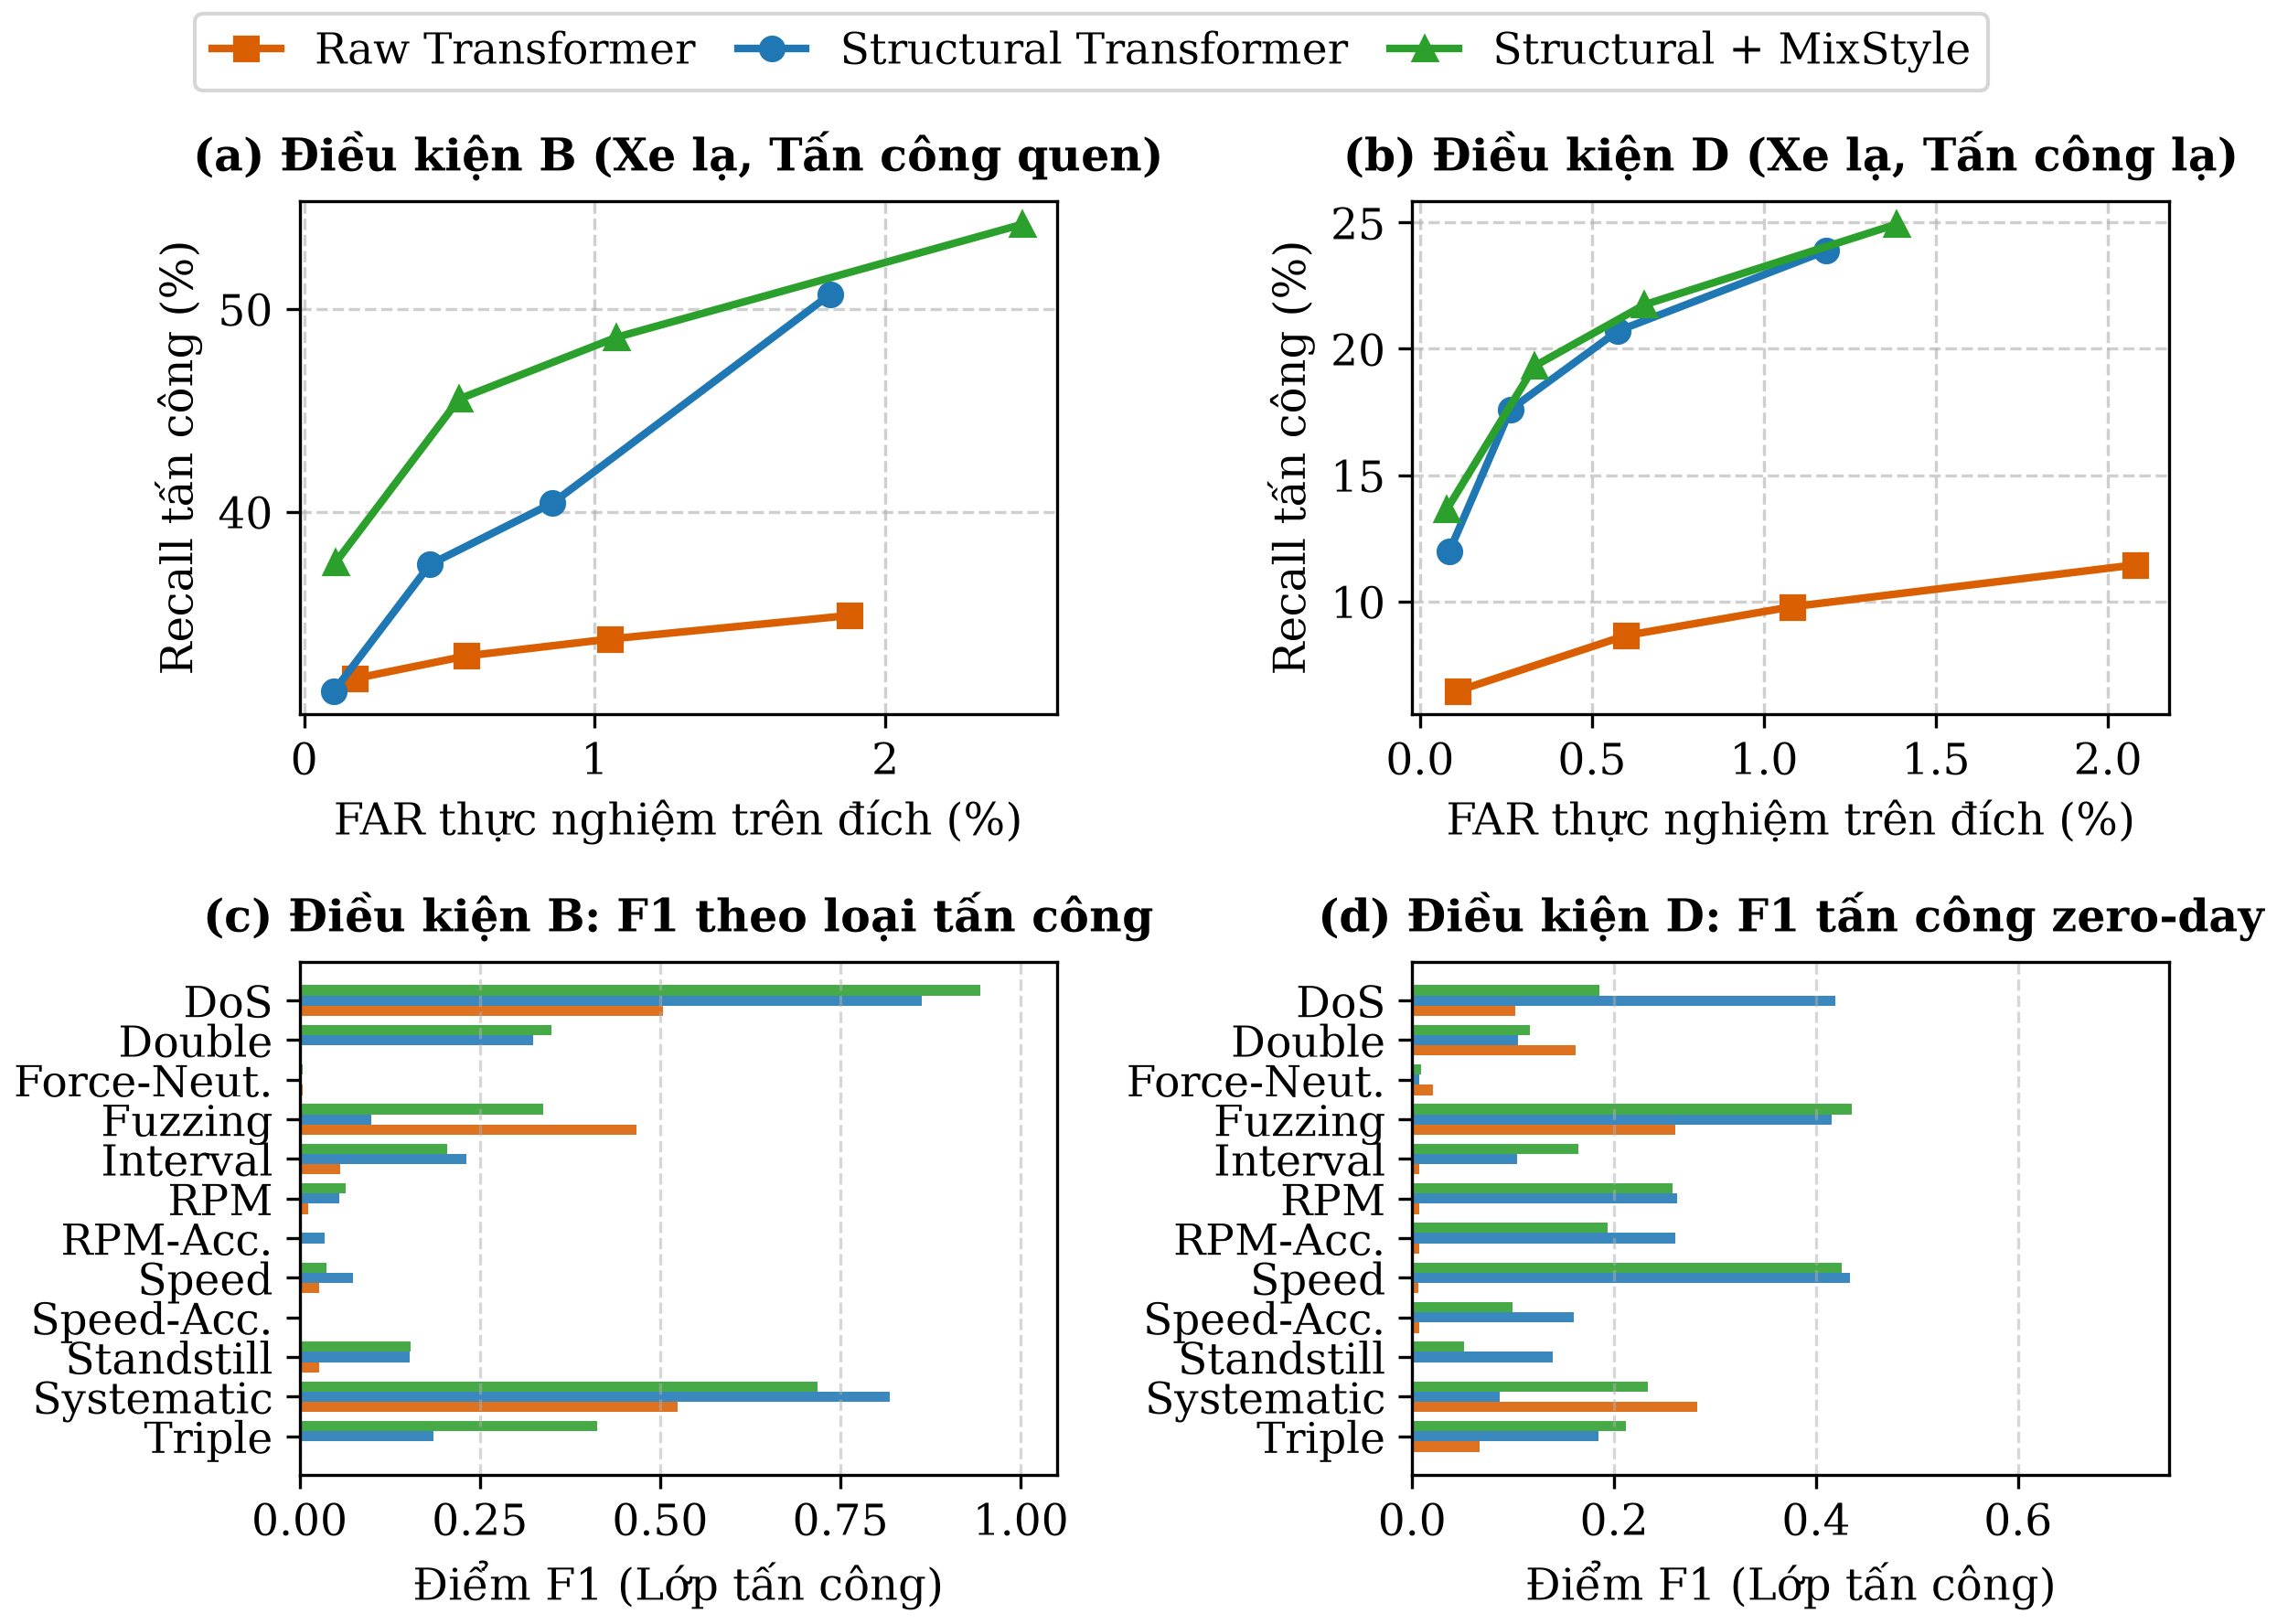
\includegraphics[width=0.80\textwidth]{figs/calibration_recovery_comparison.png}
\caption[Đánh giá khôi phục điểm vận hành qua hiệu chuẩn nền lành tính xe đích]{Đánh giá khôi phục điểm vận hành qua hiệu chuẩn nền lành tính xe đích: (a)--(b) Đường cong Recall theo ngân sách FAR thực nghiệm tại $K=500$; (c)--(d) Điểm F1 theo từng loại tấn công ở điều kiện B và D tại ngân sách khởi động $K=500, \alpha=1{,}0\%$ (đối chiếu chi tiết tại Bảng~\ref{tab:benign-calibration-summary}).}\label{fig:calibration-recovery}
\end{figure}

{\renewcommand{\arraystretch}{0.84}
\begin{table}[htbp]\centering\footnotesize\setlength{\tabcolsep}{4pt}
\caption[Hiệu năng hiệu chuẩn nền lành tính theo ngân sách khởi động $K$]{Hiệu năng khôi phục điểm vận hành qua hiệu chuẩn nền lành tính không giám sát theo $K \in \{200, 500, 1000\}$ (tiền tố khởi động gộp đa tệp $N_{\text{pool}} \in [3.539, 6.000]$ cửa sổ tại $K=500$; trung bình bốn tập; giá trị trong ngoặc là trung bình ba xe đích khử lặp)}\label{tab:benign-calibration-summary}
\begin{tabular}{P{0.7cm}P{0.9cm}P{1.7cm}P{3.1cm}P{2.2cm}P{1.4cm}P{1.2cm}P{1.2cm}}
\toprule
ĐK & $K$ & Ngân sách & Pipeline & Recall (3-xe) & FAR (\%) & AP & F1\\\midrule
B & 200 & 1,0\% & Structural + MixStyle & 0,4734 (0,4949) & 1,2163 & 0,5832 & 0,5344\\
B & 500 & 0,1\% & Raw & 0,3177 (0,3743) & 0,1727 & 0,3803 & 0,3810\\
B & 500 & 0,1\% & Structural & 0,3117 (0,3460) & 0,1024 & 0,5607 & 0,4227\\
B & 500 & 0,1\% & Structural + MixStyle & \textbf{0,3749} (0,3999) & 0,1077 & \textbf{0,5845} & \textbf{0,4955}\\
B & 500 & 1,0\% & Raw & 0,3373 (0,3922) & 1,0509 & 0,3803 & 0,3788\\
B & 500 & 1,0\% & Structural & 0,4042 (0,4303) & 0,8545 & 0,5607 & 0,4748\\
B & 500 & 1,0\% & Structural + MixStyle & \textbf{0,4859} (0,5042) & 1,0752 & \textbf{0,5845} & \textbf{0,5450}\\
B & 1000 & 0,1\% & Structural + MixStyle & 0,4002 (0,4246) & 0,0999 & 0,5864 & 0,5150\\
B & 1000 & 1,0\% & Structural + MixStyle & \textbf{0,5141} (0,5218) & 0,9710 & \textbf{0,5864} & \textbf{0,5697}\\
\midrule
D & 200 & 1,0\% & Structural + MixStyle & 0,2124 (0,2283) & 0,5086 & 0,3680 & 0,2863\\
D & 500 & 0,1\% & Raw & 0,0645 (0,0834) & 0,1087 & 0,1692 & 0,1018\\
D & 500 & 0,1\% & Structural & 0,1196 (0,1403) & 0,0845 & 0,3411 & 0,1793\\
D & 500 & 0,1\% & Structural + MixStyle & \textbf{0,1363} (0,1611) & 0,0772 & \textbf{0,3702} & \textbf{0,2026}\\
D & 500 & 1,0\% & Raw & 0,0979 (0,1257) & 1,0818 & 0,1692 & 0,1195\\
D & 500 & 1,0\% & Structural & 0,2071 (0,2255) & 0,5750 & 0,3411 & 0,2728\\
D & 500 & 1,0\% & Structural + MixStyle & \textbf{0,2175} (0,2340) & 0,6529 & \textbf{0,3702} & \textbf{0,2852}\\
D & 1000 & 1,0\% & Structural + MixStyle & 0,2211 (0,2375) & 0,7078 & 0,3728 & 0,2869\\
\bottomrule\end{tabular}
\end{table}}

{\renewcommand{\arraystretch}{0.84}
\begin{table}[htbp]\centering\footnotesize\setlength{\tabcolsep}{4pt}
\caption[Đối chứng hiệu chuẩn nền lành tính cho đối thủ và bộ lọc sự kiện $m$-trong-$n$]{So sánh hiệu quả hiệu chuẩn nền lành tính trên các mô hình đối thủ và tác động của bộ lọc sự kiện trượt $m$-trong-$n$ ($K=500$, tiền tố khởi động gộp đa tệp $N_{\text{pool}} \in [3.539, 6.000]$ cửa sổ, ngân sách FAR $1{,}0\%$)}\label{tab:cal-baselines-mofn}
\begin{tabular}{P{4.2cm}P{0.9cm}P{1.6cm}P{1.6cm}P{1.6cm}P{1.65cm}P{1.3cm}}
\toprule
Phương pháp / Quy tắc & ĐK & Recall & FAR (\%) & F1 & Precision & AP\\\midrule
CANBERT+ adapted (Calib. $K=500$) & B & 0,2428 & 20,5601 & 0,1078 & -- & 0,0997\\
CANBERT+ adapted (mean-pool) & B & 0,1183 & 1,8902 & 0,1562 & -- & 0,1665\\
CANLP-char-DNN adapted (Calib. $K=500$) & B & 0,6578 & 68,2462 & 0,0794 & -- & 0,0564\\
CANLP-char-DNN adapted (mean-pool) & B & 0,1402 & 1,7714 & 0,1835 & -- & 0,2011\\
Raw TF (1-of-1) & B & 0,3373 & 1,0509 & 0,3788 & -- & 0,3803\\
Structural TF (1-of-1) & B & 0,4042 & 0,8545 & 0,4748 & 0,6846 & 0,5607\\
Structural + MixStyle (1-of-1) & B & 0,4859 & 1,0752 & 0,5450 & 0,6603 & 0,5845\\
Structural + MixStyle (2-of-3) & B & 0,4911 & \textbf{0,2234} & 0,5903 & 0,8496 & --\\
Structural + MixStyle (2-of-5) & B & \textbf{0,5351} & 0,5491 & \textbf{0,6141} & 0,7704 & --\\
Structural + MixStyle (3-of-5) & B & 0,4926 & \textbf{0,1387} & 0,5947 & \textbf{0,9131} & --\\
\midrule
Structural + MixStyle (1-of-1) & D & 0,2175 & 0,6529 & 0,2852 & 0,4857 & 0,3702\\
Structural + MixStyle (2-of-3) & D & 0,1995 & \textbf{0,1160} & 0,2820 & 0,5738 & --\\
Structural + MixStyle (3-of-5) & D & 0,1919 & \textbf{0,0575} & 0,2747 & \textbf{0,6091} & --\\
\bottomrule\end{tabular}
\end{table}}

Từ Bảng~\ref{tab:benign-calibration-summary}, Bảng~\ref{tab:cal-baselines-mofn} và Hình~\ref{fig:calibration-recovery}, nghiên cứu rút ra năm kết luận định lượng:
\begin{enumerate}
    \item \textbf{Khôi phục ưu thế vận hành và thống kê đuôi:} Tại $K=500, \alpha=1{,}0\%$ ở điều kiện B, các đối thủ trực tiếp dưới dạng chấm điểm khung tin chuẩn (\code{CANBERT+} có FAR $20{,}56\%$, \code{CANLP-char-DNN} có FAR $68{,}25\%$) bị vỡ ngân sách nghiêm trọng do hiện tượng trôi dạt phân vị. Đáng chú ý, khi bổ sung cơ chế gộp trung bình (\code{mean}-pooling) theo cửa sổ thời gian cho các mô hình đối thủ, tỷ lệ báo động giả của chúng được kéo giảm hiệu quả về mức $\approx 1{,}8\%$ (Bảng~\ref{tab:cal-baselines-mofn}), song chỉ số chất lượng xếp hạng AP ($0{,}1665$ đối với CANBERT+ và $0{,}2011$ đối với CANLP-char-DNN) vẫn tụt hậu rất xa so với Structural Transformer ($0{,}5607$) và Structural+MixStyle ($0{,}5845$), chứng minh rằng ưu thế phân tách vượt trội của hệ thống xuất phát từ bản thân không gian biểu diễn cấu trúc chứ không phải do bước gom cụm hậu xử lý. Trong khi đó, Structural đạt recall $40{,}42\%$ ($\text{FAR}=0{,}8545\%$) và Structural+MixStyle đạt $48{,}59\%$ (3 xe đích $50{,}42\%$, $\text{FAR}=1{,}0752\%$). Trên toàn bộ các tập đối chuẩn, FAR thực nghiệm trung bình đạt $\le 1{,}08\%$, nhưng có độ phân tán lớn giữa các xe: Set~3 đạt FAR thấp nhất $0{,}22\%$, trong khi Set~4 chạm mức xấu nhất $2{,}00\%$ (gấp đôi ngân sách danh định $1{,}0\%$ do tính không dừng của xe đích). Điều này cho thấy quy trình tiền tố giúp cải thiện đáng kể khả năng kiểm soát FAR trung bình chứ không bảo đảm tuyệt đối trên mọi xe cá thể. Ở $K=500, \alpha=0{,}1\%$, $K\alpha = 0{,}5 < 1$ gây phương sai đuôi lớn hơn mức $K=1000$ ($K\alpha = 1$). Phân rã theo từng tập (Bảng~\ref{tab:cal-k-per-set}, Phụ lục~\ref{app:sensitivity}) cho thấy hiệu quả tăng mạnh ở Set~1 ($88{,}44\%$) và Set~3 ($53{,}14\%$) nhưng khiêm tốn ở Set~4 ($19{,}74\%$).
    \item \textbf{Lọc sự kiện trượt $m$-trong-$n$:} Ở tốc độ bus $1.000$--$2.000$~khung/giây ($56.250$--$112.500$ cửa sổ/giờ), bộ lọc \code{2-of-3} cắt FAR B gần $5\times$ xuống $0{,}2234\%$ (Precision $0{,}8496$, Recall $49{,}11\%$), còn \code{3-of-5} hạ FAR B xuống $0{,}1387\%$ (Precision $0{,}9131$) và FAR D xuống $0{,}0575\%$ (không chứng minh định vị từng frame). Đáng chú ý, ngay cả ở mức FAR cửa sổ $0{,}1387\%$, với mật độ $56.250\text{--}112.500$ cửa sổ/giờ trên đường truyền thực tế, hệ thống vẫn ghi nhận khoảng $78\text{--}156$ cửa sổ cảnh báo/giờ; do đó việc đánh giá tần suất báo động theo giờ và độ trễ phát hiện sự kiện thực tế nằm ngoài phạm vi phân tích theo cửa sổ của luận văn.
    \item \textbf{Rủi ro đầu độc khởi động:} Tiêm $1\%, 2\%, 5\%$ mẫu tấn công vào đoạn khởi động $K=500$ của Structural+MixStyle làm recall B ($\alpha=1{,}0\%$) tụt từ $48{,}59\%$ xuống $47{,}24\%$, $44{,}95\%$ và $32{,}85\%$ (ở $\alpha=0{,}1\%$, chỉ $1\%$ nhiễm bẩn làm recall giảm hơn một nửa từ $37{,}49\%$ xuống $16{,}06\%$ và xuống $5{,}33\%$ ở $5\%$).
    \item \textbf{Phân rã theo kiểu tấn công:} Tại B ($K=500, 1{,}0\%$), Structural+MixStyle đạt recall $92{,}42\%$ trên DoS (F1 $0{,}9438$ vs Raw $0{,}5040$) và $72{,}35\%$ trên Systematic (F1 $0{,}7177$), trong khi \code{force-neutral} ($0{,}38\%$) và \code{speed} ($7{,}31\%$) vẫn thấp; ở D, \code{speed} đạt $40{,}13\%$ (Raw $1{,}03\%$) và \code{fuzzing} $39{,}71\%$.
    \item \textbf{Kiểm chứng ngoại bộ ($K=500, \alpha=0{,}1\%$, 3 seed):} \textit{Opel Astra (DoS)} giảm FAR xuống $0{,}271\% \pm 0{,}266\%$ (Structural) và $0{,}167\% \pm 0{,}079\%$ (MixStyle) với recall $1{,}0000$; \textit{Renault Clio (DoS)} giữ recall $0{,}9984$ và triệt tiêu FAR về $0{,}0000\%$ (Raw $0{,}0508\%$ benign); \textit{CICIoV2024} thoát suy biến FAR $100\%$ ($0{,}047\%$ và $0{,}086\%$) nhưng phương sai seed rất lớn (Structural recall $0{,}3336 \pm 0{,}5242$, AP $0{,}9172 \pm 0{,}0711$; MixStyle recall $0{,}0001 \pm 0{,}0002$ ở $0{,}1\%$ và $0{,}3229 \pm 0{,}5593$ ở $1{,}0\%$); \textit{CAN\_MIRGU} giữ FAR $0{,}087\%\text{--}0{,}094\%$ ($1{,}135\%\text{--}1{,}236\%$ trên benign) nhưng recall chỉ đạt $0{,}0065\text{--}0{,}0072$ ($0{,}0275\text{--}0{,}0308$ ở $1{,}0\%$).
\end{enumerate}

\noindent\textbf{Đối chứng chỉ dùng dữ liệu nền đích ($K=500$), thách thức Target-Only và tính bổ trợ kiến trúc:} Một câu hỏi mang tính phản biện cốt lõi là: \textit{Một khi hệ thống đã chấp nhận cho phép thu thập $K=500$ cửa sổ lành tính đầu phiên trên xe đích để hiệu chuẩn, liệu việc huấn luyện Transformer phức tạp trên các xe nguồn có thực sự cần thiết hay không?} Kết quả đối chứng tổng hợp tại Bảng~\ref{tab:target-only-summary} (chi tiết tại Mục~\ref{subsec:target-only-k500}, Bảng~\ref{tab:target-only-k500}, Phụ lục~\ref{app:sensitivity}), trong đó các bộ dò thuần xe đích cùng xuất phát từ tập tiền tố khởi động gộp đa tệp $N_{\text{pool}} = \sum k_i \in [3.539, 6.000]$ cửa sổ lành tính (gom $k_i = \min(500, \lfloor L_{\text{benign}}^{(i)}/2\rfloor)$ từ mỗi tệp thử nghiệm, bảo đảm cùng ngân sách quan sát với quy trình hiệu chuẩn Transformer). Trong đó, \code{IsolationForest} khớp mô hình và chọn ngưỡng phân vị in-sample trên toàn bộ $N_{\text{pool}}$, còn \code{Split-Mahalanobis} áp dụng cơ chế tách đôi (\textit{split-warmup}) chia ngân sách thành $N_{\text{fit}} \in [1.770, 3.000]$ cửa sổ đầu (250 cửa sổ đầu mỗi tệp) để ước lượng $\mu, \Sigma$ và $N_{\text{cal}} \in [1.770, 3.000]$ cửa sổ tiếp theo (250 cửa sổ sau mỗi tệp) để chọn ngưỡng phân vị out-of-sample chống rò rỉ nội mẫu. Kết quả đưa ra câu trả lời vừa thách thức vừa làm sáng tỏ bản chất của bài toán:
\begin{itemize}
    \item \textit{Ưu thế phân tách của biểu diễn cấu trúc không cần nhãn nguồn:} Trên các bộ dò bất thường thuần xe đích không dùng dữ liệu nguồn (0 mẫu nguồn, 0 nhãn tấn công), \code{Split-Mahalanobis St60} (áp dụng cơ chế split-warmup gom 250 cửa sổ đầu mỗi tệp làm tập ước lượng $\mu, \Sigma$ với độ co ngót $0{,}1$ và 250 cửa sổ sau làm tập chọn ngưỡng phân vị out-of-sample) đạt chất lượng xếp hạng AP vượt trội hơn hẳn Transformer nguồn (Điều kiện B: $0{,}7048$ so với $0{,}5845$; Điều kiện D: $0{,}7605$ so với $0{,}3702$). Thậm chí, ở ngân sách $\alpha=0{,}1\%$ điều kiện D, \code{IsolationForest St60} đạt Recall $24{,}05\%$ (FAR $0{,}122\%$), vượt trội hơn mức $13{,}63\%$ (FAR $0{,}077\%$) của Structural+MixStyle đã hiệu chuẩn. Tuy nhiên, sự vượt trội cục bộ này đi kèm các đánh đổi vận hành cốt lõi: (i) FAR thực nghiệm của \code{IsolationForest} tại ngân sách danh định $\alpha=0{,}1\%$ bị trôi lên $0{,}122\%$ ở D và $0{,}195\%$ ở B ($1{,}2\times\text{--}1{,}9\times$ ngân sách, trong khi Transformer giữ chặt ở $0{,}077\%\text{--}0{,}108\%$), và khi nới ngân sách lên $\alpha=1{,}0\%$, FAR thực tế của cây vọt lên $1{,}713\%\text{--}2{,}708\%$ (vỡ ngân sách $1{,}7\times\text{--}2{,}7\times$), đồng thời recall ở điều kiện B thua sút Transformer ($31{,}74\%$ vs $37{,}49\%$ tại $\alpha=0{,}1\%$ và $38{,}89\%$ vs $48{,}59\%$ tại $\alpha=1{,}0\%$); (ii) Về mặt triển khai nhúng, việc phải khớp không giám sát (fit) toàn bộ 200 cây cô lập ngay trên xe tại mỗi chu kỳ khởi động đòi hỏi tài nguyên bộ nhớ SRAM đáng kể để lưu trữ cấu trúc đồ thị con trỏ cây, trái ngược với mô hình mạng nơ-ron có trọng số tĩnh nạp sẵn (ROM) chỉ cần cập nhật một ngưỡng phân vị vô hướng duy nhất; và (iii) Dù chuỗi điểm bất thường của cây về nguyên tắc vẫn có thể ghép nối với bộ lọc sự kiện trượt $m$-trong-$n$, việc khảo nghiệm kết hợp hậu lọc chuỗi trên các bộ dò Target-Only ở cùng mức FAR thực nghiệm là hướng nghiên cứu mở đầy hứa hẹn cho các hệ IDS lai trong tương lai. Kết quả này chứng minh rằng không gian đặc trưng cấu trúc 30 chiều (tương ứng 60 chiều thống kê mean+std) tự thân nó đã sở hữu tính phân tách bất thường nội tại rất mạnh mà không nhất thiết phải có sự giám sát của nhãn nguồn.
    \item \textit{Sự vỡ ngân sách vùng đuôi của bộ ước lượng đa chiều và vai trò bộ nén 1D:} Tuy nhiên, điểm yếu chết người của các mô hình mật độ không gian cao như Mahalanobis 60 chiều (ngay cả khi fit trên toàn bộ tiền tố gộp $N_{\text{fit}} \approx 1.770\text{--}3.000$ cửa sổ của xe đích) là \textbf{mất kiểm soát hoàn toàn tỷ lệ báo động giả vùng đuôi}: tại ngân sách $\alpha=0{,}1\%$ và $1{,}0\%$, FAR thực nghiệm của \code{Split-Mahalanobis St60} trượt lên $1{,}225\%\text{--}4{,}999\%$ ở B và $1{,}530\%\text{--}7{,}564\%$ ở D (vỡ ngân sách gấp $5\times\text{--}15\times$). Nguyên nhân bắt nguồn từ việc ma trận hiệp phương sai 60 chiều cực kỳ nhạy cảm với hiện tượng phi dừng giữa các chuyến lái, tự tương quan chuỗi và phân phối phi Gauss đuôi nặng của luồng dữ liệu CAN thực tế.
    \item \textit{Tính bổ trợ kiến trúc (Architectural Complementarity):} Ngược lại, bộ mã hóa phân biệt học từ miền nguồn (được hiện thực hóa ở đây bởi Transformer 2 lớp) đóng vai trò như một \textbf{bộ nén thông tin rủi ro 1 chiều}: nén chuỗi 64 vector 30 chiều phức tạp thành một giá trị logit vô hướng duy nhất. Điều này cho thấy lợi thế thực nghiệm then chốt về số lượng tham số cần ước lượng trên dữ liệu đích: trong khi các mô hình mật độ không giám sát cũng suy biến chuỗi thành điểm dị thường 1D, chúng buộc phải ước lượng toàn bộ tham số biểu diễn trực tiếp trên tiền tố đích không dừng (ma trận hiệp phương sai đối xứng $60 \times 60$ gồm $1.830$ tham số độc lập cộng $60$ tham số kỳ vọng cho Mahalanobis, hoặc cấu trúc cây cho IsolationForest), dẫn đến mất ổn định đuôi phân phối; ngược lại, bộ mã hóa nguồn đóng băng Transformer sở hữu $0$ tham số biểu diễn cần fit trên miền đích và chỉ yêu cầu ước lượng một ngưỡng vô hướng duy nhất $\tau$ trên dòng logit 1D, mang lại hiệu quả kiểm soát FAR đuôi ổn định hơn trong các kịch bản thử nghiệm.
\end{itemize}

{\renewcommand{\arraystretch}{0.85}
\begin{table}[htbp]\centering\footnotesize
\caption[So sánh đối chứng Transformer nguồn và bộ phát hiện thuần xe đích]{So sánh đối chứng hiệu năng giữa Transformer huấn luyện nguồn (sau hiệu chuẩn $K=500$) và các bộ phát hiện thuần không giám sát chỉ dùng dữ liệu nền đích ($K=500$, không dữ liệu nguồn) tại Điều kiện B và D}\label{tab:target-only-summary}
\begin{tabular}{P{4.4cm}P{0.8cm}P{1.0cm}P{1.6cm}P{1.8cm}P{1.6cm}P{1.6cm}}
\toprule
Phương pháp & ĐK & $\alpha$ & Recall & FAR (\%) & F1 & AP \\ \midrule
Structural + MixStyle (Calib.) & B & 0,1\% & 0,3749 & \textbf{0,108} & 0,4955 & 0,5845 \\
Structural + MixStyle (Calib.) & B & 1,0\% & 0,4859 & \textbf{1.075} & 0,5450 & 0,5845 \\
IsolationForest St60 (Target-Only) & B & 0,1\% & 0,3174 & 0,195 & 0,3888 & 0,5989 \\
IsolationForest St60 (Target-Only) & B & 1,0\% & 0,3889 & 2.708 & 0,3575 & 0,5989 \\
Split-Mahalanobis St60 (Target-Only)& B & 0,1\% & \textbf{0,6581} & 1.225 & \textbf{0,6829} & \textbf{0,7048} \\
Split-Mahalanobis St60 (Target-Only)& B & 1,0\% & 0,7007 & 4.999 & 0,5968 & \textbf{0,7048} \\
\midrule
Structural + MixStyle (Calib.) & D & 0,1\% & 0,1363 & \textbf{0,077} & 0,2026 & 0,3702 \\
Structural + MixStyle (Calib.) & D & 1,0\% & 0,2175 & \textbf{0,653} & 0,2852 & 0,3702 \\
IsolationForest St60 (Target-Only) & D & 0,1\% & 0,2405 & 0,122 & 0,3238 & 0,5287 \\
IsolationForest St60 (Target-Only) & D & 1,0\% & 0,3931 & 1.713 & 0,4041 & 0,5287 \\
Split-Mahalanobis St60 (Target-Only)& D & 0,1\% & \textbf{0,6244} & 1.530 & \textbf{0,6344} & \textbf{0,7605} \\
Split-Mahalanobis St60 (Target-Only)& D & 1,0\% & 0,7193 & 7.564 & 0,5547 & \textbf{0,7605} \\
\bottomrule
\end{tabular}
\end{table}}
Đồng thời, cần nhấn mạnh sự phân biệt giữa tiền tố khởi động một chuyến lái đơn lẻ ($K=500$ cửa sổ, tương ứng $\approx 16\text{--}32$ giây khi nổ máy tĩnh) và tiền tố gộp đa tệp trong giao thức benchmark ngoại tuyến ($N_{\text{pool}} = \sum K_{\text{valid}} \in [3.539, 6.000]$ cửa sổ): việc gộp $N_{\text{pool}}$ đảm bảo $N_{\text{pool}}\alpha \ge 3{,}54 > 1$ tại $\alpha=0{,}1\%$; trong khi nếu triển khai trên một chuyến lái độc lập với $K=500$, điều kiện $K\alpha = 0{,}5 < 1$ đòi hỏi tích lũy qua nhiều phiên khởi động hoặc vận hành ở ngân sách $\alpha \ge 0{,}5\%$ kết hợp bộ lọc trượt $m$-trong-$n$.

\FloatBarrier

\noindent\textbf{Trả lời trực diện RQ5a:} Cơ chế hiệu chuẩn nền lành tính không giám sát với ngân sách khởi động nhỏ ($K=500$) khôi phục thành công điểm vận hành thực tế cho bộ mã hóa nguồn trên xe đích (kéo giảm FAR từ $>52\%$ xuống $\approx 0{,}85\%\text{--}1{,}08\%$ tại $\alpha=1{,}0\%$), đồng thời vượt trội các phương pháp thuần xe đích (Target-Only) ở khả năng kiểm soát chặt chẽ tỷ lệ báo động giả vùng đuôi nhờ tận dụng Transformer như một bộ nén rủi ro 1 chiều ổn định.


\subsection{Đánh giá các cơ chế thích ứng và triệt tiêu cấp đặc trưng (RQ5b)}\label{sec:feature-invariance}
Phần này đánh giá các phương pháp tiếp cận hướng tới việc triệt tiêu sự khác biệt phân phối trực tiếp trong không gian biểu diễn ẩn $z_k \in \mathbb{R}^{64}$ thay vì chỉ can thiệp ngưỡng phân loại ở đầu ra.

\subsubsection{Điều chuẩn phân phối ẩn bằng MixStyle}\label{subsec:eval-mixstyle}
Bảng~\ref{tab:mixstyle-ad} đánh giá hiệu năng \code{Structural + MixStyle} qua 12 lượt huấn luyện (4 set $\times$ 3 seed; các đối chiếu mở rộng gồm bảng sáu mô hình, linear probe, 57 bản ghi ngoại bộ và chi phí xử lý tại các Bảng~\ref{tab:mixstyle-six}, \ref{tab:mixstyle-probe}, \ref{tab:mixstyle-external} Mục~\ref{subsec:app-mixstyle}, Phụ lục~\ref{app:sensitivity}).

{\renewcommand{\arraystretch}{0.85}
\begin{table}[htbp]\centering\footnotesize
\caption[Hiệu năng kết hợp MixStyle qua bốn điều kiện A--D dưới ngưỡng nguồn]{So sánh hiệu năng của Structural Transformer kết hợp kỹ thuật MixStyle qua bốn điều kiện A--D dưới ngưỡng nguồn (trung bình theo hạt giống rồi trọng số đều bốn tập; FAR theo phần trăm)}\label{tab:mixstyle-ad}
\begin{tabular}{P{1cm}P{4.3cm}P{1.6cm}P{2cm}P{1.5cm}P{1.5cm}}
\toprule
A--D & Pipeline & Recall & FAR (\%) & AP & F1\\\midrule
A & Raw & 0,6167 & 0,1158 & 0,7312 & 0,7258\\
A & Structural & 0,5886 & 0,0817 & 0,7483 & 0,7072\\
A & Structural + MixStyle & 0,6675 & 0,0827 & 0,7784 & 0,7701\\
B & Raw & 0,8541 & 65,3014 & 0,3781 & 0,3000\\
B & Structural & 0,7383 & 52,4615 & 0,5554 & 0,2435\\
B & Structural + MixStyle & 0,8194 & 64,5387 & 0,5815 & 0,2298\\
C & Raw & 0,2101 & 0,0919 & 0,2661 & 0,2314\\
C & Structural & 0,2230 & 0,0758 & 0,2928 & 0,2600\\
C & Structural + MixStyle & 0,2838 & 0,0781 & 0,3620 & 0,3317\\
D & Raw & 0,6614 & 67,9829 & 0,1648 & 0,1213\\
D & Structural & 0,6445 & 54,6434 & 0,3357 & 0,2069\\
D & Structural + MixStyle & 0,6982 & 66,9915 & 0,3658 & 0,1600\\
\bottomrule\end{tabular}
\end{table}}

Ở tiêu chí chính B, MixStyle nâng recall so với Structural thêm $+8{,}11$ điểm phần trăm ($0{,}8194$ vs $0{,}7383$, vẫn thấp hơn Raw $0{,}8541$) và nâng AP lên $0{,}5815$, nhưng kéo FAR tăng $+12{,}08$ điểm phần trăm lên $64{,}54\%$ (trên A/C/D mức tăng recall so với Raw chỉ xuất hiện lần lượt ở $2/4$, $4/4$ và $1/4$ tập). Trên các đối chứng mở rộng tại Mục~\ref{subsec:app-mixstyle}, Phụ lục~\ref{app:sensitivity} (các Bảng~\ref{tab:mixstyle-six}, \ref{tab:mixstyle-probe}, \ref{tab:mixstyle-external} ), MixStyle không giảm khả năng giải mã xe (probe đạt $0{,}9527$ vs $0{,}9488$) và trên tập ngoại bộ chỉ giảm nhẹ FAR Renault Clio DoS ($0{,}1886\% \to 0{,}1467\%$) trong khi tăng FAR Opel Astra lên $33{,}43\%$. Do đó MixStyle chỉ đóng vai trò tăng cường thứ tự xếp hạng trước hiệu chuẩn ngưỡng chứ không giải quyết độc lập chuyển dịch miền.

\subsubsection{Học đa nguồn LOVO kết hợp đối kháng có điều kiện}\label{subsec:eval-lovo}
Bảng~\ref{tab:multisource-lovo} và Hình~\ref{fig:multisource-lovo} trình bày kết quả 48 lượt huấn luyện đa nguồn LOVO (Mục~\ref{subsec:method-lovo}) với ngưỡng chọn từ validation của 3 xe nguồn (FAR nguồn $\le 99{,}87/100\text{k}$).

\begin{figure}[htbp]
\centering
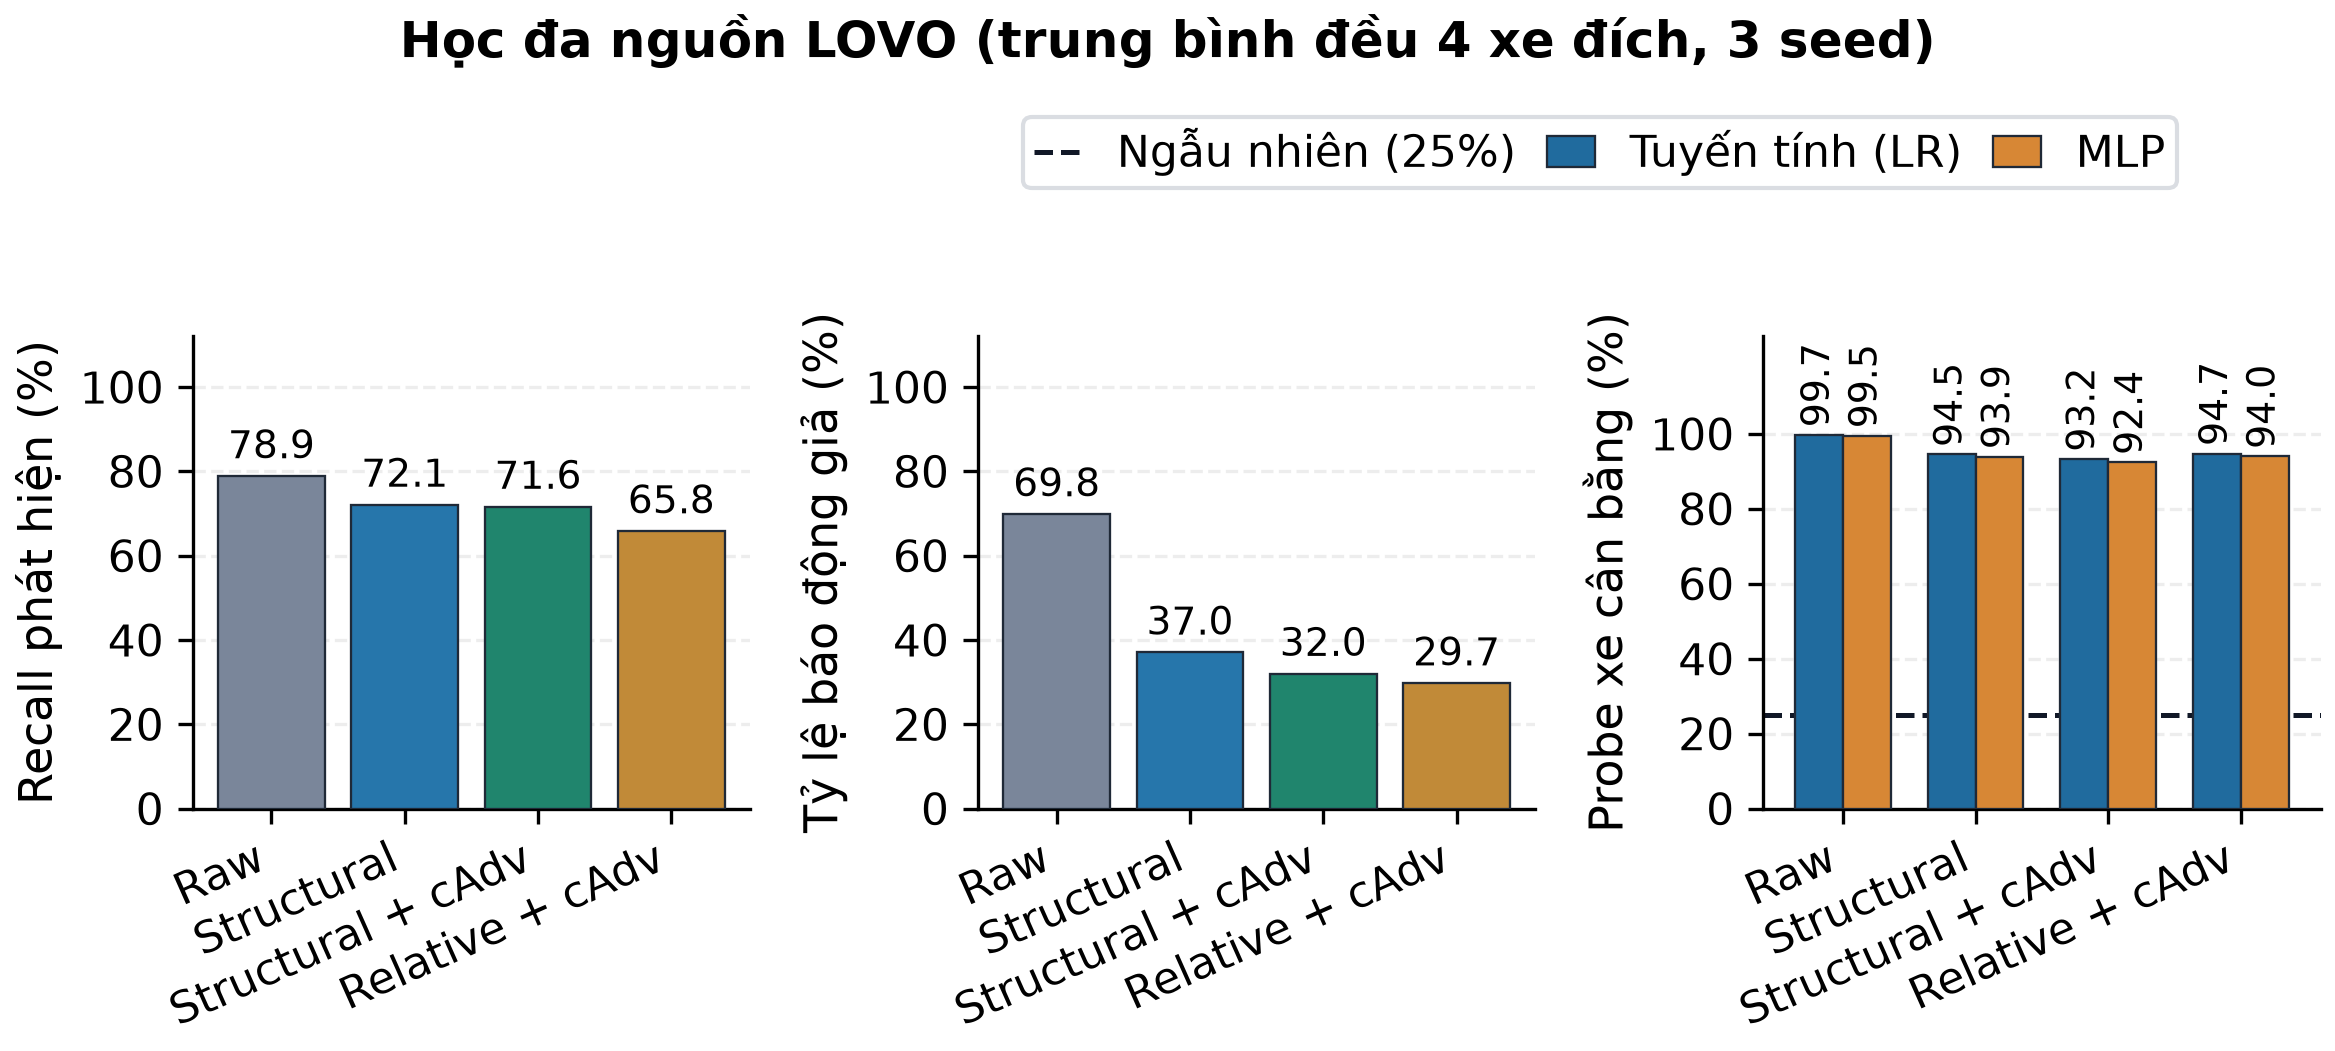
\includegraphics[width=0.80\textwidth]{figs/multisource_lovo_overview.png}
\caption[Hiệu năng học đa nguồn LOVO và mức độ rò rỉ danh tính xe]{Hiệu năng học đa nguồn LOVO (trung bình đều 4 xe giữ ngoài $\times$ 3 seed) tại ngưỡng validation nguồn và khả năng giải mã xe bằng probe (mức cơ hội $25\%$).}\label{fig:multisource-lovo}
\end{figure}

{\renewcommand{\arraystretch}{0.85}
\begin{table}[htbp]\centering\footnotesize\setlength{\tabcolsep}{4pt}
\caption[Kết quả học đa nguồn LOVO với đối kháng miền có điều kiện]{Kết quả học đa nguồn giữ ngoài một xe (LOVO) kèm nhánh đối kháng có điều kiện (48 lượt huấn luyện; trọng số đều bốn xe đích; ngưỡng chọn từ nguồn)}\label{tab:multisource-lovo}
\begin{tabular}{P{2.8cm}P{1.4cm}P{2.6cm}P{1.2cm}P{1.2cm}P{1.8cm}P{1.8cm}}
\toprule
Phương pháp & Recall & FAR /100k (\%) & AP & F1 & Probe xe (LR/MLP) & Probe atk (LR) \\ \midrule
Raw & 0,7885 & 69835,3 (69,84\%) & 0,2196 & 0,2182 & 99,74\% / 99,47\% & 61,51\% \\
Structural & \textbf{0,7211} & 37022,5 (37,02\%) & \textbf{0,6020} & 0,4073 & 94,49\% / 93,89\% & 80,47\% \\
Structural + cAdv & 0,7161 & 31974,5 (31,97\%) & 0,5970 & \textbf{0,4254} & \textbf{93,22\%} / \textbf{92,36\%} & \textbf{81,11\%} \\
Relative + cAdv & 0,6579 & \textbf{29721,1} (29,72\%) & 0,5764 & 0,4148 & 94,74\% / 93,96\% & 79,94\% \\
\midrule
\multicolumn{7}{P{13.6cm}}{\footnotesize \textit{Ghi chú:} Giá trị in đậm thể hiện kết quả tốt nhất trong các mô hình dựa trên cấu trúc đề xuất (Raw có Recall 0,7885 nhưng suy biến với FAR lên tới 69,84\% và AP chỉ 0,2196). Probe xe thấp hơn thể hiện ít rò rỉ danh tính xe hơn.}\\
\bottomrule
\end{tabular}
\end{table}} (Raw $0{,}2196$) và nhánh đối kháng~\cite{ganin2016dann} có điều kiện (\code{cAdv}) giảm FAR nguồn xuống $31{,}97\%$ ($\text{F1}=0{,}4254$), FAR phân rã theo xe vẫn bộc lộ sự mất cân bằng giữa các nền tảng: \textit{Traverse} đạt $0{,}058\%$ (recall $51{,}35\%$, AP $0{,}6193$) và \textit{Impala} $0{,}473\%$ (recall $54{,}26\%$, AP $0{,}6314$), nhưng \textit{Silverado} tăng lên $47{,}46\%$ (recall $85{,}46\%$, AP $0{,}6485$) và \textit{Forester} tới $79{,}91\%$ (recall $95{,}40\%$, AP $0{,}4890$). Đáng chú ý, biến thể \code{Relative + cAdv} (22D, loại bỏ 8 byte payload tuyệt đối như định nghĩa tại Mục~\ref{subsec:method-lovo}) cắt giảm thêm FAR nguồn xuống mức thấp nhất trong nhóm đa nguồn ($29{,}72\%$) trong khi vẫn bảo toàn khả năng giải mã tấn công ở mức cao ($79{,}94\%$ probe tấn công, Bảng~\ref{tab:multisource-lovo}, Phụ lục~\ref{app:sensitivity}). Tuy nhiên, mức độ tồn lưu thông tin xe của toàn bộ các biến thể đối kháng vẫn ở mức cao ($93{,}22\%\text{--}94{,}74\%$ probe LR), khẳng định rằng tối ưu đối kháng đơn thuần không thể xóa bỏ hoàn toàn ranh giới giữa các miền phương tiện.

\subsubsection{Làm trắng nền lành tính, triệt tiêu tuyến tính LEACE/INLP8 và điểm năng lượng Mahalanobis}\label{subsec:eval-whitening}
Trên 96 pipeline hậu nghiệm (12 encoder LOVO đóng băng $\times$ 8 nhánh, trích tổng cộng 54.231 cửa sổ lành đối chứng trên cả 4 xe đích gồm $19.774 + 8.968 + 20.239 + 5.250$ cửa sổ; mỗi xe dành riêng một bản ghi lành tính độc lập kèm kiểm tra lọc trùng mã băm SHA-256 loại 740 cửa sổ trùng SHA-256; Mục~\ref{subsec:method-whitening}), Bảng~\ref{tab:benign-invariant-main} và Hình~\ref{fig:benign-invariant} đối chiếu hiệu quả làm trắng nền lành, xóa tuyến tính LEACE/INLP8 và điểm năng lượng Mahalanobis $E_{\text{white}}$.

\begin{figure}[htbp]
\centering
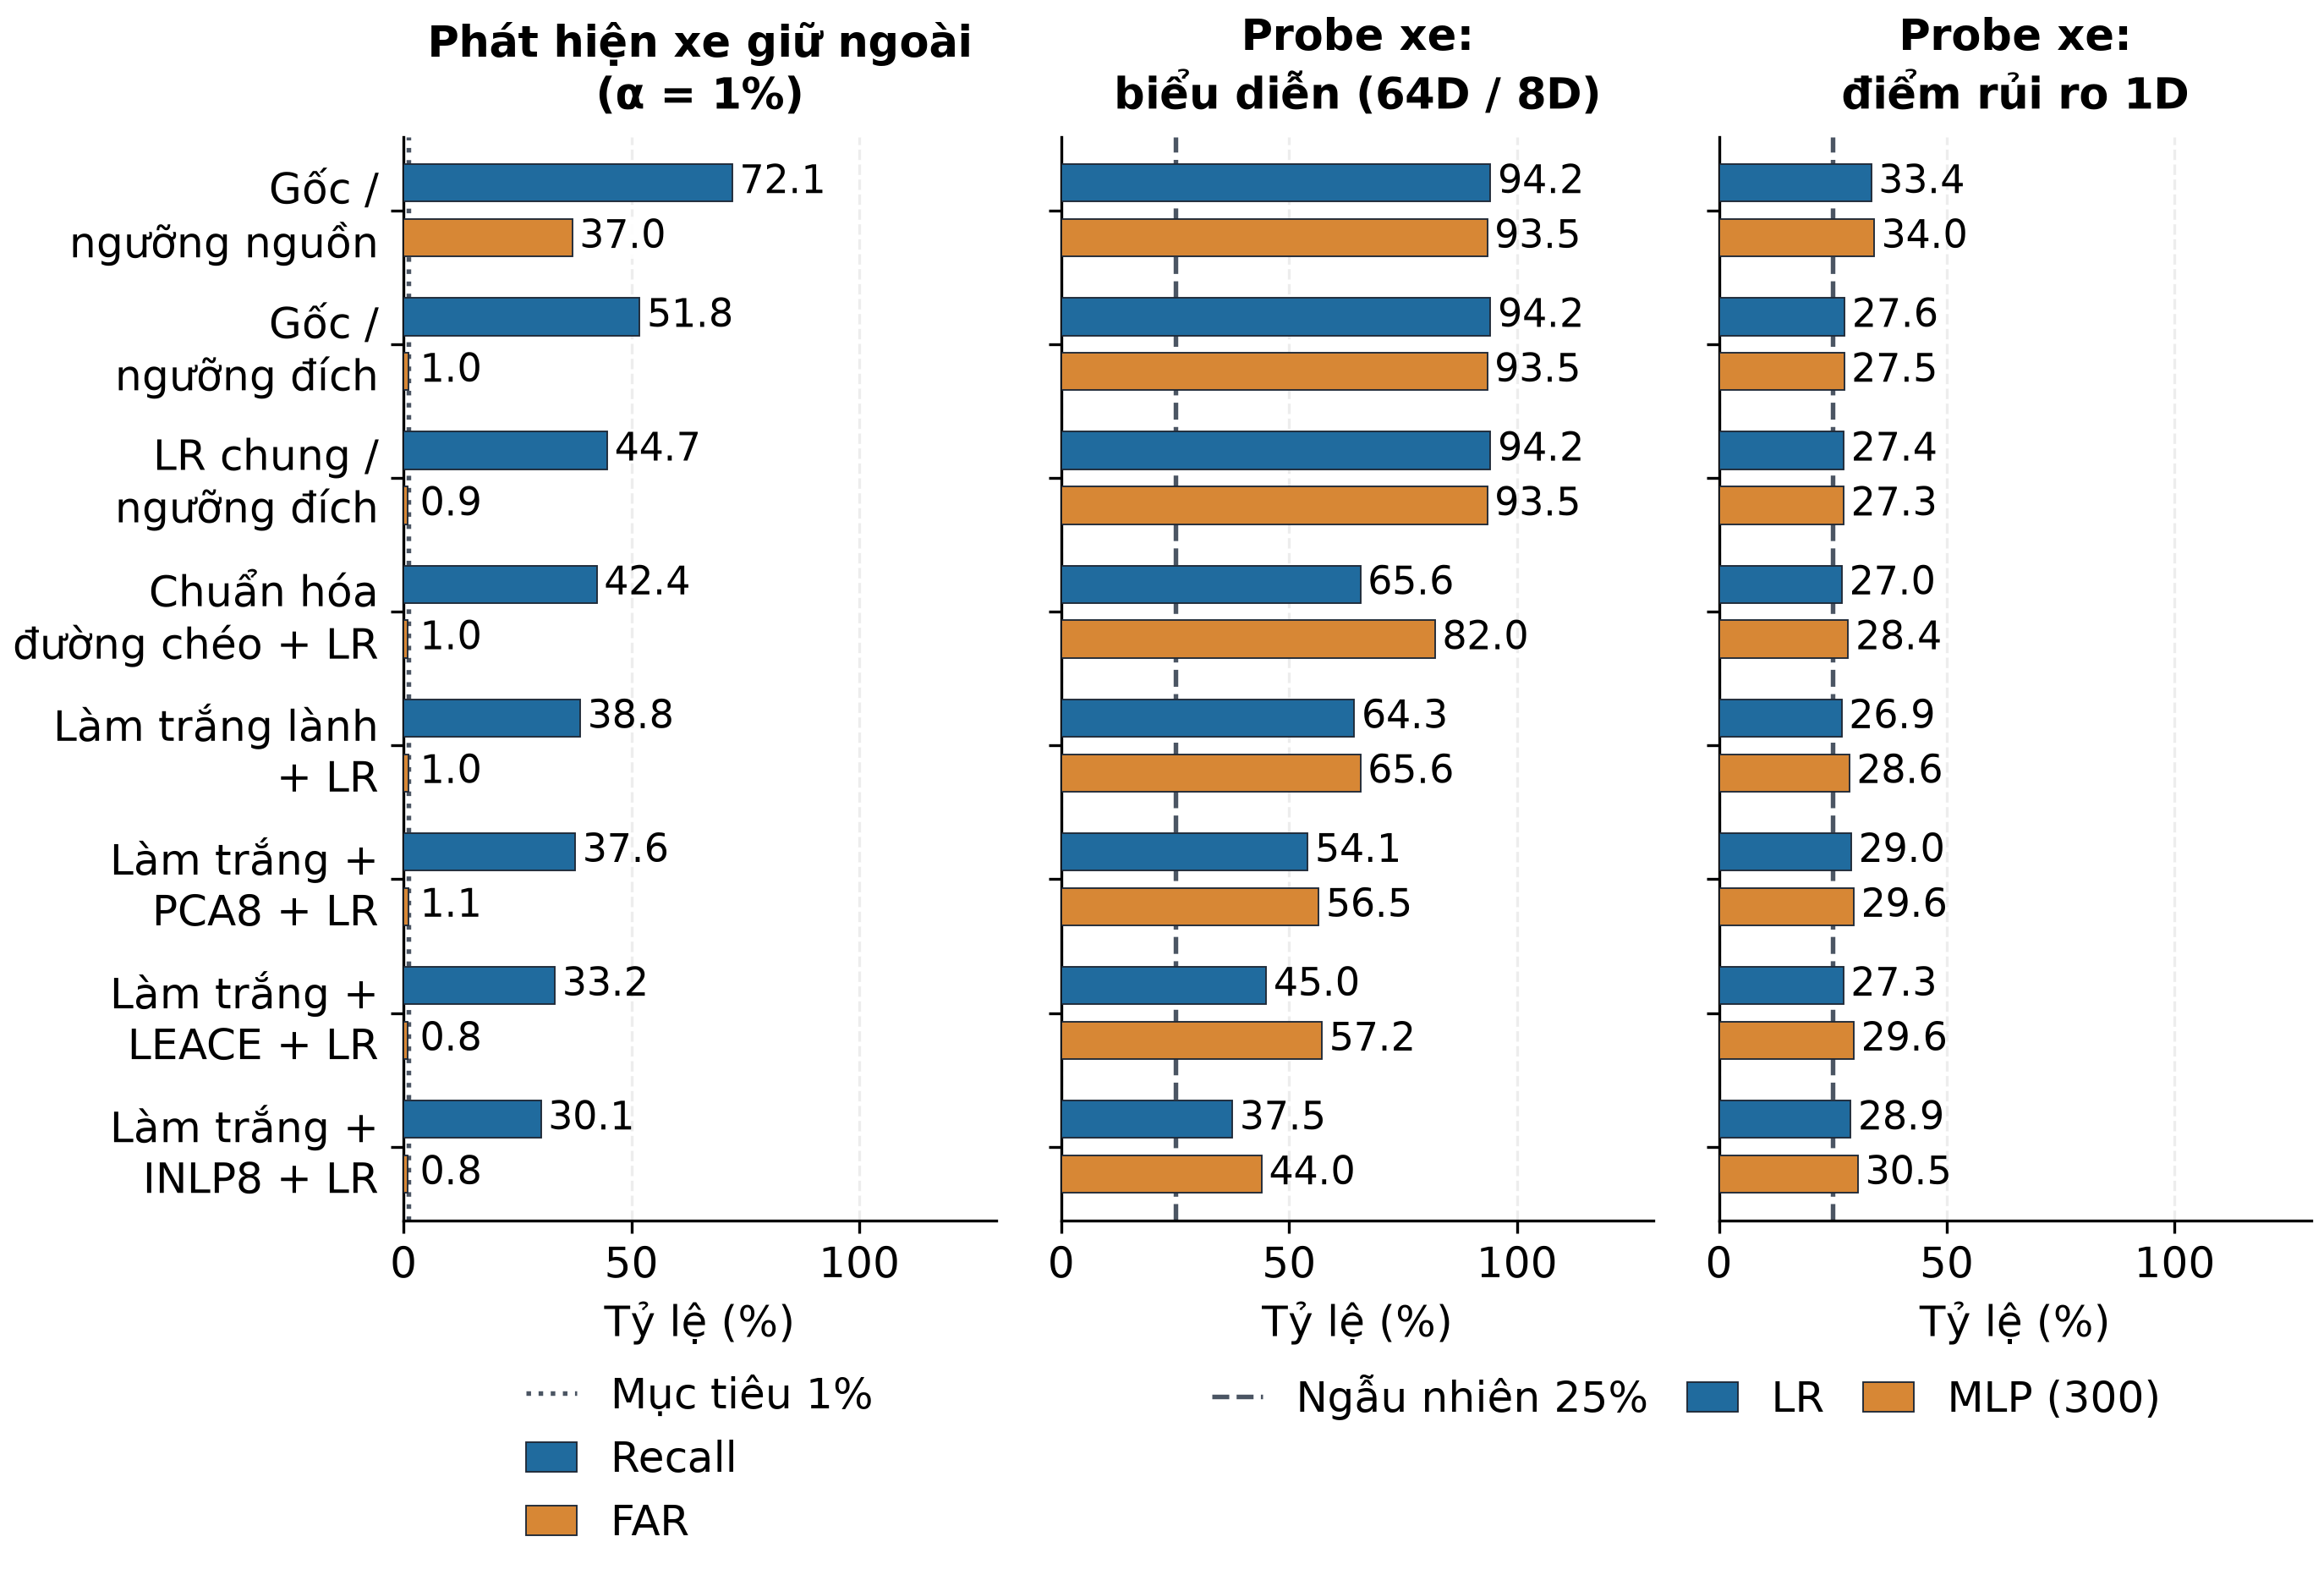
\includegraphics[width=0.80\textwidth]{figs/benign_invariant_overview.png}
\caption[Đối chiếu phát hiện tấn công và thăm dò tuyến tính sau làm trắng--xóa khái niệm]{Đối chiếu đồng thời phát hiện tấn công ($\alpha=1\%$, lọc trùng mã băm SHA-256), probe 4 xe trên biểu diễn đặc trưng (không gian 64D gốc / chiếu 8D dư đối với PCA8 và INLP8) và probe trên điểm rủi ro 1 chiều (mức cơ hội $25\%$).}\label{fig:benign-invariant}
\end{figure}

{\renewcommand{\arraystretch}{0.84}
\begin{table}[htbp]\centering\footnotesize\setlength{\tabcolsep}{3.5pt}
\caption[So sánh làm trắng nền lành tính kết hợp xóa tuyến tính và điểm năng lượng]{So sánh hiệu năng làm trắng nền lành tính kết hợp triệt tiêu khái niệm tuyến tính (LEACE/INLP8) và điểm bất thường năng lượng $E_{\text{white}}$ ($\alpha=1{,}0\%$ chuẩn hóa, lọc trùng mã băm SHA-256)}\label{tab:benign-invariant-main}
\begin{tabular}{P{3.0cm}P{1.1cm}P{1.3cm}P{1.1cm}P{1.1cm}P{1.7cm}P{1.6cm}P{1.5cm}}
\toprule
Phương pháp & Recall & FAR (\%) & F1 & AP & Probe biểu diễn (LR / MLP300) & MLP 1.500 vòng & Risk 1D (LR) \\ \midrule
Original / source thresh. & 0,7211 & 37,001 & 0,4096 & 0,6042 & 94,18\% / 93,46\% & 93,46\% & 33,40\% \\
Original / target thresh. & \textbf{0,5180} & 1,009 & \textbf{0,6032} & 0,6042 & 94,18\% / 93,46\% & -- & 27,58\% \\
Shared LR / target thresh. & 0,4469 & 0,889 & 0,5362 & 0,5544 & 94,18\% / 93,46\% & -- & 27,38\% \\
Benign diag + LR & 0,4239 & 0,990 & 0,5152 & 0,5243 & 65,63\% / 81,99\% & -- & 26,99\% \\
Benign whitening + LR & 0,3876 & 1,036 & 0,4705 & 0,4852 & 64,29\% / 65,63\% & -- & 26,92\% \\
Whitening + PCA8 + LR & 0,3765 & 1,100 & 0,4361 & 0,4603 & 54,08\% / 56,48\% & 53,68\% & 29,03\% \\
Whitening + LEACE + LR & 0,3321 & \textbf{0,844} & 0,4065 & 0,4242 & 44,96\% / 57,19\% & 57,17\% & \textbf{27,30\%} \\
Whitening + INLP8 + LR & 0,3013 & \textbf{0,844} & 0,3750 & 0,3715 & \textbf{37,53\%} / \textbf{43,97\%} & \textbf{42,01\%} & 28,90\% \\
\midrule
$E_{\text{white}}$ ($\alpha=0{,}1\%$) & 0,4606 & \textbf{0,297} & \textbf{0,5918} & \textbf{0,6172} & -- & -- & -- \\
$E_{\text{white}}$ ($\alpha=1{,}0\%$) & 0,6008 & 3,831 & 0,5323 & \textbf{0,6172} & -- & -- & -- \\
\midrule
\multicolumn{8}{P{13.8cm}}{\footnotesize \textit{Ghi chú:} Cột Probe biểu diễn đo trên không gian nhúng gốc cho các hàng trên, và đo trên không gian chiếu dư đối với các hàng PCA và INLP. Hàng \code{Original / source thresh.} có sai khác số học nhỏ so với hàng \code{Structural} ở Bảng~\ref{tab:multisource-lovo} (FAR $37{,}001\%$ so với $37{,}02\%$, AP $0{,}6042$ so với $0{,}6020$, Probe xe $94{,}18\%$ so với $94{,}49\%$) do bảng này áp dụng bộ lọc lọc trùng mã băm SHA-256 loại bỏ $740$ cửa sổ trùng mã băm SHA-256 trên tập dữ liệu lành đối chứng. Giá trị in đậm ở nửa trên thể hiện hiệu năng tốt nhất trong nhóm phân loại nhị phân có giám sát với $\alpha=1{,}0\%$; nửa dưới thể hiện điểm năng lượng không giám sát $E_{\text{white}}$ (đạt Recall 0,6008 ở $\alpha=1{,}0\%$ và FAR 0,297\% ở $\alpha=0{,}1\%$; do được tính trực tiếp từ khoảng cách Mahalanobis trên không gian nhúng mà không qua đầu phân loại nhị phân logit, cột Risk 1D được đánh dấu gạch ngang ---).}\\
\bottomrule
\end{tabular}
\end{table}}

Ba phát hiện chính từ Bảng~\ref{tab:benign-invariant-main} và Hình~\ref{fig:benign-invariant}: (1) \textbf{Ngụy tạo bất biến trên điểm rủi ro 1D:} Gập biểu diễn xuống điểm rủi ro 1D kéo probe xe về $27{,}30\%\text{--}28{,}90\%$ trong khi embedding 64D vẫn giữ $94{,}18\%$; (2) \textbf{Đánh đổi xóa tuyến tính và phần dư phi tuyến:} LEACE/INLP8 giảm probe tuyến tính 64D xuống $44{,}96\%/37{,}53\%$ (vượt PCA8 $54{,}08\%$, giữ probe tấn công $79{,}05\%\text{--}81{,}44\%$), nhưng làm recall tụt từ $51{,}80\%$ xuống $33{,}21\%/30{,}13\%$ và MLP 1.500 vòng vẫn giải mã được $57{,}17\%/42{,}01\%$; (3) \textbf{Điểm năng lượng $E_{\text{white}}$:} Đạt $\text{AP}=0{,}6172$ cao nhất; tại $\alpha=0{,}1\%$ đạt recall $46{,}06\%$, FAR $0{,}297\%$ ($297{,}3/100\text{k}$), F1 $0{,}5918$ (Impala $59{,}09\%$, Silverado $53{,}97\%$, Traverse $52{,}33\%$, Forester $18{,}85\%$), nhưng ở $\alpha=1{,}0\%$ FAR trượt lên $3{,}83\%$ do tự tương quan chuỗi CAN.

\noindent\textbf{Trả lời trực diện RQ5b:} Các kỹ thuật thích ứng miền cấp đặc trưng (MixStyle, LOVO-cAdv, LEACE/INLP8) giúp cải thiện biên phân tách và giảm thiểu một phần dấu ấn phương tiện, nhưng không thể xóa bỏ triệt để ranh giới miền trong không gian nhúng mà không làm suy giảm tín hiệu phát hiện tấn công do tồn dư phi tuyến sâu sắc giữa cấu trúc bus và chữ ký bất thường.

\section{Chi phí xử lý thực nghiệm và các đe dọa tính hợp lệ}
\subsection{Chi phí xử lý trên máy thực nghiệm và phân rã độ trễ}\label{sec:runtime}
Bảng~\ref{tab:runtime-decomp} cô lập chi phí xử lý ba thành phần trên CPU/GPU (\code{batch=1}, 20 cửa sổ tiền tố + 900 cửa sổ kiểm chuẩn độ trễ); Do MixStyle chuyển về phép đồng nhất (identity) khi suy luận, chi phí suy luận của \code{Structural + MixStyle} hoàn toàn tương đương \code{Structural}. Chi tiết phân rã ba thành phần được tổng hợp tại Bảng~\ref{tab:runtime-decomp} và kiểm toán độ phức tạp tĩnh tại Bảng~\ref{tab:model-complexity-audit} (Phụ lục~\ref{app:sensitivity}).

{\renewcommand{\arraystretch}{0.86}
\begin{table}[htbp]\centering\footnotesize
\caption{Phân rã độ trễ xử lý ba thành phần theo từng cửa sổ $W=64$ trên CPU và GPU ($N=900$, \code{batch=1}, đơn vị ms)}\label{tab:runtime-decomp}
\begin{tabular}{P{1.6cm}P{2.5cm}P{2.5cm}P{2.5cm}P{2.8cm}}
\toprule
Thiết bị & Đọc CSV (Median) & Trích xuất kép 28D+30D (Median) & Suy luận Structural (Median) & Tổng E2E Structural (Median / P95) \\ \midrule
CPU & 1,083 & 3,036 & 0,731 & 4,830 / 6,231 \\
CUDA & 0,932 & 2,285 & 1,150 & 4,402 / 5,291 \\
\bottomrule
\end{tabular}
\end{table}}

Thời gian suy luận thuần của \code{Structural Transformer} trên CPU chỉ đạt $0{,}731\text{ ms}$ (tương đương Raw $0{,}768\text{ ms}$, nhanh hơn CUDA $1{,}150\text{ ms}$ ở \code{batch=1}), trong khi khâu đọc CSV ($1{,}083\text{ ms}$) và trích xuất kép ($3{,}036\text{ ms}$) chiếm phần lớn chi phí E2E trong quy trình đo lường đối chuẩn (chi tiết phân rã chi phí tính toán và độ trễ được tổng hợp tại Bảng~\ref{tab:runtime-decomp}); trên bus 500~kbps ($1.000\text{--}2.000\text{ khung/giây}$) cần cộng thêm $32\text{--}64\text{ ms}$ chờ gom cửa sổ $W=64$ (tổng $\approx 37\text{--}70\text{ ms}$). Kiểm toán độ phức tạp tĩnh (Mục~\ref{subsec:complexity-audit}, Bảng~\ref{tab:model-complexity-audit}, Phụ lục~\ref{app:sensitivity}) xác nhận Structural chỉ thêm $128$ tham số ($75.298$ vs $75.170$, $+0{,}17\%$), $8.192$ MACs ($+0{,}15\%$) và $130{,}00\text{ KiB}$ RAM bảng $H_k$ (ở bản triển khai thực tế bằng C/C++ trên vi điều khiển nhúng, việc lưu trữ kiểu \texttt{uint8\_t} cho payload và mặt nạ bit giúp rút gọn bảng $H_k$ xuống chỉ còn $\approx 20{,}48\text{ KiB}$, hoàn toàn nằm trọn trong SRAM của ECU ô tô), nhẹ hơn \code{CANBERT+} ($54{,}25\text{M}$ tham số, $206{,}94\text{ MiB}$, $27{,}24\text{G}$ MACs) tới $720\times$ về tham số và $5.075\times$ về khối lượng tính toán.

\subsection{Đe dọa tính hợp lệ}\label{sec:threats-to-validity}
Khóa luận nhận diện năm nhóm đe dọa tính hợp lệ cần được xem xét khi diễn giải kết quả:
\begin{enumerate}
    \item \textbf{Hiệu lực kết cấu và thiết kế đối chuẩn đa phương tiện:}
    \begin{itemize}
        \item \textit{Đa dạng nền tảng vật lý:} Bộ đối chuẩn CTT chỉ gồm 4 dòng xe vật lý với 3 xe đích phân biệt (Subaru Forester xuất hiện lặp ở cả Tập 2 và Tập 3), và các vòng ghi chưa có siêu dữ liệu chuyến lái độc lập hoàn toàn.
        \item \textit{Sai lệch gộp và mức độ giám sát:} Nhãn nhị phân cấp cửa sổ $W=64$ không đo lường định vị khung tin hay độ trễ tiền sự cố; các mô hình baseline cấp khung tin (\code{CANLP}, \code{CANBERT+}) chịu bất lợi quy nạp lớn khi đối chuẩn dưới cùng một ngưỡng FAR cố định so với pooling trung bình.
        \item \textit{Phạm vi kiểm thử ngoại bộ:} Đánh giá trên 57 bản ghi ngoại bộ sử dụng mô hình neo huấn luyện từ Tập 1 (xe nguồn Chevrolet Impala), chưa bao quát toàn bộ 4 tập huấn luyện nguồn.
    \end{itemize}

    \item \textbf{Độ ổn định vùng đuôi và tính dừng của luồng dữ liệu:}
    \begin{itemize}
        \item \textit{Dịch chuyển tiên nghiệm lớp:} Việc lấy mẫu reservoir áp trần $1.000$ cửa sổ/lớp tạo tỷ lệ lớp nhân tạo cân bằng ($50:50$), lệch xa phân bố tấn công thực tế ($0{,}03\%\text{--}8\%$), thúc đẩy hiện tượng bão hòa logit và trôi dạt ngưỡng.
        \item \textit{Kích thước mẫu khởi động đơn chuyến:} Tại ngân sách khắt khe $\alpha=0{,}1\%$, một chuyến đi đơn lẻ với $K=500$ cửa sổ ($K\alpha = 0{,}5 < 1$) nhạy cảm với phương sai đuôi; phân vị chỉ ổn định vững chắc khi gộp đa phiên ($N_{\text{pool}} \ge 3.539$) hoặc vận hành ở $\alpha \ge 0{,}5\%$.
        \item \textit{Tự tương quan chuỗi:} Luồng dữ liệu CAN thực tế có tính tự tương quan thời gian mạnh và tính phi dừng giữa các chuyến lái, do đó các chặn phân vị IID không cấu thành cam kết phân phối tự do trong mọi điều kiện vận hành.
    \end{itemize}

    \item \textbf{Giới hạn của phép thăm dò tuyến tính:}
    \begin{itemize}
        \item \textit{Cảnh báo hội tụ tối ưu:} Phép thăm dò tuyến tính ghi nhận cảnh báo hội tụ ở một số ô tham số (98/576 ô ở LOVO, 133 ô ở làm trắng) do đặc tính phân tách gần như hoàn hảo của không gian đặc trưng.
        \item \textit{Tồn dư phi tuyến:} Việc triệt tiêu thông tin xe trên bộ thăm dò tuyến tính hoặc trên điểm rủi ro 1 chiều không đồng nghĩa với tính bất biến toàn diện, khi bộ giải mã MLP phi tuyến vẫn trích xuất được $42{,}01\%\text{--}57{,}17\%$ nhãn xe.
    \end{itemize}

    \item \textbf{Tính hậu nghiệm và tính toàn vẹn thời gian:}
    \begin{itemize}
        \item \textit{Bản chất phân tích chẩn đoán:} Các phân tích MixStyle, LOVO và làm trắng hiệp phương sai được thiết kế theo hướng chẩn đoán hậu nghiệm sau khi quan sát hiện tượng phân kỳ ở 4 tập đối chuẩn.
        \item \textit{Xáo trộn dấu thời gian:} Hiện tượng đảo ngược dấu thời gian dưới mili-giây trên CTT buộc mô hình chính phải vận hành ở chế độ thuần nội dung, chưa thay thế hoàn toàn đánh giá trên luồng bus vật lý thời gian thực.
    \end{itemize}

    \item \textbf{Khoảng cách triển khai trên vi điều khiển nhúng:}
    \begin{itemize}
        \item \textit{Độ trễ gom cửa sổ:} Mặc dù thời gian suy luận thuần trên CPU chỉ tốn $0{,}731\text{ ms}$, việc gom đủ $W=64$ khung tin trên đường truyền 500~kbps đòi hỏi độ trễ tích lũy vật lý $32\text{--}64\text{ ms}$.
        \item \textit{Ràng buộc phần cứng thực tế:} Các phép đo lường trên máy trạm chưa phản ánh đầy đủ xung đột hàng đợi bus, tranh chấp bộ nhớ hay hạn chế ngắt thời gian thực trên vi điều khiển chuyên dụng của ô tô.
    \end{itemize}
\end{enumerate}

\section{Tóm tắt chương}
Chương này đã triển khai toàn diện chuỗi thực nghiệm đối chứng khẳng định và chẩn đoán biểu diễn trên 60 đơn vị mô hình IDS độc lập qua bốn điều kiện chuyển giao A--D và 136 tệp nhật ký có dấu thời gian đơn điệu nghiêm ngặt. Các phân tích cắt bỏ 10 biến thể biểu diễn và quét độ nhạy kích thước cửa sổ $W \in \{32, 64, 128\}$ đã bóc tách rõ vai trò sống còn của các nhóm đặc trưng thống kê cục bộ và biến thiên tải trọng. Kết quả đối chứng xác lập sự phân kỳ sâu sắc giữa chất lượng phân tách độc lập ngưỡng (chỉ số AP được cải thiện vượt trội $+17{,}74$ điểm phần trăm) và sự trôi dạt nghiêm trọng của điểm vận hành tĩnh đóng băng từ nguồn (FAR tăng vọt lên $>52\%$). Đồng thời, các thí nghiệm thăm dò tuyến tính có kiểm soát (Linear Probe) và kiểm thử ngoại bộ trên 57 bản ghi độc lập cung cấp bằng chứng chẩn đoán vững chắc về hiện tượng đan xen đặc trưng: các tín hiệu hình thái khung tin (DLC/mặt nạ) và mật độ bus vừa mang dấu ấn nhận diện kiến trúc xe sâu sắc, vừa là kênh thông tin cốt lõi để phát hiện bất thường.

Trên cơ sở chẩn đoán đó, chương đã đánh giá thấu đáo các giải pháp thích ứng miền cấp đặc trưng và cấp vận hành nhằm khôi phục điểm làm việc thực tế cho hệ thống. Mặc dù các kỹ thuật chuẩn hóa phân phối ẩn (MixStyle), học đối kháng đa nguồn (LOVO-cAdv) và triệt tiêu khái niệm tuyến tính (LEACE/INLP8) giúp nới rộng biên phân tách và hạ thấp dấu ấn nhận diện xe trên điểm rủi ro 1 chiều, chúng không thể xóa bỏ hoàn toàn ranh giới giữa các miền phương tiện do sự tồn dư phi tuyến sâu sắc của cấu trúc bus. Trái lại, quy trình hiệu chuẩn nền lành tính tiền tố ngắn không giám sát ($K=500$ cửa sổ, tương ứng $16\text{--}32$ giây khởi động tĩnh) kết hợp bộ lọc sự kiện trượt $m$-trong-$n$ đã khôi phục thành công điểm vận hành thực tế cho bộ phát hiện nguồn trên xe đích, kiểm soát tỷ lệ báo động giả vùng đuôi chặt chẽ hơn hẳn các mô hình mật độ thuần xe đích (Target-Only). Toàn bộ các kết luận khoa học, giá trị thực tiễn, giới hạn và định hướng mở rộng hệ thống được tổng kết tại \hyperref[chap:conclusion]{Phần Kết luận và hướng phát triển}.

\chap{Kết luận và hướng phát triển}\label{chap:conclusion}
\sect{Tổng kết các kết quả nghiên cứu chính}
Qua quá trình thực nghiệm đối chứng nghiêm ngặt trên nhiều điều kiện chuyển giao đa xe và các bộ dữ liệu ngoại bộ, khóa luận rút ra các kết luận khoa học cốt lõi sau:

\textbf{Trả lời RQ1 (Về hiệu năng chuyển giao đa xe và sự phân kỳ ngưỡng):}
Giả thuyết cho rằng biểu diễn cấu trúc giúp tự động tăng độ nhạy (Recall) trên xe đích lạ ở cửa sổ $W=64$ dưới một ngưỡng tĩnh đóng băng từ nguồn ($\text{FAR} \le 100/100.000$) không được ủng hộ bởi thực nghiệm. Tại ngưỡng nguồn, Structural đạt recall 73,83\%, thấp hơn Raw khoảng 11,59 điểm phần trăm (85,41\%), đồng thời tỷ lệ báo động giả trên xe đích tăng cao ($\text{FAR} = 52{,}46\%$). Tuy nhiên, khi đánh giá chất lượng phân tách độc lập với ngưỡng quyết định cố định, biểu diễn Structural thể hiện ưu thế vượt trội: Average Precision (AP) ở điều kiện B tăng vọt từ 0,3781 lên 0,5554 (+17,74 điểm phần trăm chênh lệch ghép cặp; +17,73 điểm phần trăm chênh lệch trung bình so với Raw và vượt xa CANBERT+ 0,0970). Hiện tượng tỷ lệ báo động giả cao khi chuyển xe thực chất bắt nguồn từ sự trôi dạt phân phối logit (\textit{threshold shift}) giữa các hãng xe. Điều này chứng minh rằng việc đánh giá chuyển giao zero-shot trên mạng CAN phải tách biệt rõ ràng giữa chất lượng xếp hạng độc lập ngưỡng (AP) và hiệu năng vận hành tại ngưỡng tĩnh; việc khôi phục điểm vận hành khả thi trên xe đích đòi hỏi các cơ chế thích ứng và hiệu chuẩn được khảo sát trong RQ5.

\textbf{Trả lời RQ2 (Về vai trò của các thành phần trong biểu diễn cấu trúc):}
Nghiên cứu chứng minh rằng việc loại bỏ CAN-ID thô một cách đơn thuần là không đủ để tạo ra một biểu diễn chuyển giao tốt; thực tế, bỏ ID khỏi mô hình thô làm AP điều kiện B sụt giảm nghiêm trọng từ 0,3781 xuống 0,2200. Các thành phần trong biểu diễn cấu trúc mang lại những đánh đổi rõ rệt: nhóm thống kê cục bộ (tần suất và thứ tự xuất hiện của ID trong cửa sổ) đóng vai trò sống còn đối với chất lượng xếp hạng và độ nhạy phát hiện bất thường (cắt bỏ thống kê cục bộ làm AP điều kiện B rơi tự do từ 0,5554 xuống 0,2894). Trong khi đó, việc loại bỏ byte payload tuyệt đối và chỉ giữ lại động học biến thiên $\Delta$payload giúp giải phóng mô hình khỏi nguy cơ quá khớp vào chữ ký tấn công nguồn, nâng mạnh hiệu năng phát hiện tấn công zero-day ở điều kiện C (AP đạt 0,4730 so với 0,2661 của Raw).

\textbf{Trả lời RQ3 (Về mức độ độc lập đặc thù xe và hiện tượng đan xen đặc trưng):}
Phép đo thăm dò tuyến tính (\textit{Linear Probe}) chỉ ra rằng biểu diễn Structural chỉ làm giảm nhẹ khả năng giải mã danh tính xe từ 0,9925 xuống 0,9488 (4,37 điểm phần trăm), vẫn cao hơn rất nhiều so với mức cơ hội ngẫu nhiên 0,2500. Phân tích chẩn đoán chuyên sâu bóc tách nguyên nhân rò rỉ: nhóm 10 chiều hình thái khung tin \code{dlc\_and\_masks} (gồm 9 chiều DLC và mặt nạ byte hợp lệ đạt $96{,}42\%$ cùng 1 chiều cờ hợp lệ $h_i$ đạt $27{,}46\%$) cho probe xe tổng hợp $96{,}70\%$, bên cạnh mật độ lưu lượng bus cục bộ ($75{,}65\%$) mang đậm dấu ấn kiến trúc mạng của từng hãng xe. Do hiện tượng đan xen đặc trưng (\textit{feature entanglement}), các kênh cấu trúc mang thông tin xe cũng chính là các tín hiệu nhạy bén nhất để phát hiện bất thường (probe tấn công tăng từ 0,6419 lên 0,7669). Vì vậy, việc cắt bỏ đặc trưng thô bạo sẽ phá hủy khả năng phát hiện xâm nhập. Điều này khẳng định biểu diễn cấu trúc chưa đạt được tính độc lập đặc thù xe hoàn toàn, và bài toán chuyển giao phương tiện đòi hỏi các kỹ thuật thích ứng miền như hiệu chuẩn ngưỡng thay vì kỳ vọng một biểu diễn zero-shot bất biến tuyệt đối.

\textbf{Trả lời RQ4 (Về năng lực tổng quát hóa ngoại bộ và điều kiện ứng dụng thực tế):}
Kiểm thử trên 57 bản ghi ngoại bộ độc lập (sử dụng mô hình neo huấn luyện từ Tập 1 với xe nguồn Chevrolet Impala) cho thấy khả năng chuyển giao phụ thuộc chặt chẽ vào cơ chế thu thập và hình thái tấn công. Cụ thể, hệ thống đạt hiệu năng rất cao trước các kịch bản tấn công làm xáo trộn mạnh mật độ bus thực tế: trên Renault Clio (DoS), mô hình đạt Recall 99,84\% với FAR chỉ 0,19\% tại ngưỡng nguồn và triệt tiêu về 0,00\% sau hiệu chuẩn; trên Opel Astra (DoS), hiệu chuẩn giúp duy trì Recall 100\% đồng thời kéo FAR xuống $0{,}17\% \pm 0{,}08\%$ (với biến thể kết hợp MixStyle).

Ngược lại, thực nghiệm cũng bộc lộ hai ranh giới thất bại quan trọng. Thứ nhất, trên bộ dữ liệu mô phỏng CICIoV2024, tệp lành tính có độ dài khung cố định ($\text{DLC} = 8$) kèm mật độ định danh cao ($U_k = 33{,}35 \pm 3{,}30$ so với 26,75--28,34 của CTT) khiến ngưỡng nguồn báo động giả 100\%, trong khi các tệp tấn công thiếu lưu lượng nền làm $U_k$ sụp đổ về 1,00 tạo ra phân tách nhân tạo (Recall 100\%, $\text{AP} = 0{,}9172 \pm 0{,}0711$) và gây phương sai rất lớn giữa các hạt giống sau hiệu chuẩn ($0{,}3336 \pm 0{,}5242$). Thứ hai, trên CAN-MIRGU, các cuộc tấn công mạo danh giữ nguyên chu kỳ và các pha đình chỉ không chèn khung tin khiến Recall duy trì ở mức rất thấp (0,65\%--3,08\% sau hiệu chuẩn). Các kết quả này khẳng định không thể suy diễn hiệu năng trên một bộ dữ liệu đơn lẻ thành năng lực phổ quát, đồng thời nhấn mạnh vai trò bắt buộc của kiểm toán dữ liệu đầu vào và hiệu chuẩn nền đích.

\textbf{Trả lời RQ5a (Về hiệu chuẩn ngưỡng vận hành và tính bổ trợ Target-Only):}
Quy trình hiệu chuẩn tiền tố lành tính gộp ngoại tuyến (sử dụng $\mathrm{prefix\_end}$ với ngân sách $N_{\text{pool}} \in [3.539, 6.000]$ cửa sổ) cải thiện đáng kể khả năng kiểm soát tỷ lệ báo động giả thực nghiệm trung bình: Structural+MixStyle đạt Recall $48{,}59\%$ ở ngân sách danh định $\alpha=1{,}0\%$ với FAR trung bình $\le 1{,}0752\%$, và giảm tiếp xuống FAR trung bình $\le 0{,}2234\%$ kèm Precision $84{,}96\%$ khi áp dụng bộ lọc sự kiện trượt $2\text{-of-}3$. Tuy nhiên, FAR thực nghiệm có độ phân tán giữa các xe (Set~3 đạt $0{,}22\%$ trong khi Set~4 chạm mức xấu nhất $2{,}00\%$, gấp đôi ngân sách danh định do tính không dừng). Đối chứng với các bộ phát hiện thuần không giám sát trên xe đích (Target-Only) cho thấy lợi thế thực nghiệm then chốt về số lượng tham số ước lượng: đặc trưng cấu trúc 30D mang lại khả năng phân tách hình học nội tại (giúp \code{Split-Mahalanobis St60} đạt AP $0{,}7048\text{--}0{,}7605$ không cần nguồn), nhưng các bộ ước lượng mật độ mục tiêu phải ước lượng toàn bộ ma trận hiệp phương sai đối xứng $60\times 60$ ($1.830$ tham số độc lập cộng $60$ tham số kỳ vọng) trên dữ liệu đích và làm bùng nổ FAR đuôi ($1{,}225\%\text{--}7{,}564\%$); ngược lại, bộ mã hóa nguồn Transformer sở hữu 0 tham số biểu diễn cần fit trên đích và chỉ cần hiệu chuẩn 1 ngưỡng vô hướng duy nhất $\tau$, đem lại khả năng kiểm soát FAR đuôi ổn định hơn trong thực nghiệm. Cuối cùng, kết quả đối chứng trên 136 tệp đơn điệu khẳng định rằng khi có thông tin thời gian $\Delta t$ sạch, biến thể \code{Timed Structural (32D)} cải thiện mạnh xếp hạng với AP $0{,}9359$ và hạ FAR xuống $2{,}46\%$ trên 136 tệp đơn điệu, nhưng mức $2{,}46\%$ vẫn vượt ngân sách nguồn $0{,}1\%$ gấp 24,6 lần nên vẫn cần hiệu chuẩn.

\textbf{Trả lời RQ5b (Về bất biến biểu diễn cấp đặc trưng và giới hạn triệt tiêu thông tin xe):}
Các kỹ thuật điều chuẩn phân phối ẩn (MixStyle) và học đối kháng đa nguồn (LOVO-cAdv với biến thể Relative 22D) nâng cao năng lực phân tách AP (đạt tương ứng $0{,}5815$ và $0{,}6020$) nhưng không thể triệt tiêu sự dịch chuyển ngưỡng nguồn để vận hành khả thi (FAR nguồn vẫn ở mức $29{,}72\%\text{--}64{,}54\%$). Khi kết hợp làm trắng hiệp phương sai trên lưu lượng lành tính xe đích với triệt tiêu tuyến tính LEACE hoặc rút gọn INLP8, linear probe danh tính xe trên điểm rủi ro 1D giảm về sát mức cơ hội ngẫu nhiên ($27{,}30\%\text{--}28{,}90\%$), và điểm năng lượng làm trắng ($E_{\text{white}}$) đạt AP cao nhất ($0{,}6172$). Tuy nhiên, nghiên cứu bóc tách hai giới hạn then chốt: (i) triệt tiêu tuyến tính vẫn để lại rò rỉ phi tuyến đáng kể (probe MLP 1.500 vòng còn $42{,}01\%\text{--}57{,}17\%$), và (ii) con số FAR $0{,}297\%$ của $E_{\text{white}}$ ở $\alpha=0{,}1\%$ ghi nhận trong điều kiện chia xen kẽ cửa sổ chẵn/lẻ bị ảnh hưởng bởi rò rỉ tự tương quan chuỗi thời gian, do đó chỉ mang ý nghĩa chẩn đoán khả năng xóa biểu diễn chứ chưa phải là đường ống triển khai vận hành độc lập.

\sect{Giá trị và giới hạn của nghiên cứu}
Khóa luận cung cấp một đánh giá thực nghiệm hoàn toàn tái lập, xây dựng hệ thống đối chứng biểu diễn đa tầng và phân tách tường minh giữa chất lượng xếp hạng độc lập ngưỡng với hiệu năng tại điểm vận hành cố định. Tính bất biến dưới phép đổi tên ID nhất quán được chứng minh là một thuộc tính hình thức hẹp, không đồng nghĩa với tính độc lập miền xe thực tế do hiện tượng đan xen đặc trưng. Việc báo cáo trung thực các kết quả âm tính dưới ngưỡng nguồn đóng băng ngăn chặn các kết luận ngộ nhận từ các chỉ số AP hoặc Recall cục bộ, xác lập rõ ranh giới ứng dụng thực tế của mô hình phát hiện xâm nhập nội mạng ô tô.

\sect{Hướng nghiên cứu tiếp theo}
Ưu tiên dữ liệu có chronology và phiên lái độc lập được xác minh (như bộ dữ liệu ROAD), đánh giá trên các mẫu xe mới hoàn toàn độc lập với vòng phát triển, và kiểm tra độ trễ theo sự kiện. Phát triển phương pháp làm mịn/bất biến phi tuyến có điều kiện kết hợp học đa nguồn và thích ứng trực tuyến bền vững trước đầu độc khởi động để vượt qua đánh đổi của triệt tiêu tuyến tính. Thực nghiệm nhúng phải đo tài nguyên, hàng đợi, chính sách đặt lại/eviction cho bảng $H_k$ (ignition-cycle reset và LRU cho ID 29-bit/CAN-FD 64-byte), chi phí chờ $32\text{--}64\text{ ms}$ gom cửa sổ và deadline trên phần cứng mục tiêu (ARM Cortex / Jetson Nano). Bên cạnh đó, kết quả đối chứng thuần không giám sát tại Mục~\ref{subsec:target-only-k500} cho thấy mô hình khoảng cách \code{Split-Mahalanobis St60} khai thác tiền tố lành tính xe đích đạt AP rất cao ($0{,}7048\text{--}0{,}7605$, vượt trội Transformer) nhưng bị vỡ FAR vùng đuôi gấp $5\times\text{--}15\times$, trong khi Transformer giữ FAR cực kỳ chặt chẽ nhờ không cần ước lượng tham số biểu diễn mới trên miền đích và chỉ hiệu chuẩn một ngưỡng phân vị vô hướng duy nhất. Do đó, một hướng đi giàu tiềm năng cho nghiên cứu tiếp theo là phát triển \textbf{bộ dò lai (hybrid architecture)}: kết hợp điểm mật độ Mahalanobis với điểm rủi ro Transformer đóng băng và bộ lọc sự kiện trượt $m$-trong-$n$ nhằm vừa tối ưu hóa chất lượng xếp hạng AP, vừa kiểm soát nghiêm ngặt tỷ lệ báo động giả thực tế.

\appendix
\chapter{Chi tiết tái lập và nguồn gốc bằng chứng}\label{app:reproducibility}
\section{Nguồn gốc bằng chứng và quy mô thực nghiệm}\label{sec:app-provenance}
Ma trận chính gồm 60 đơn vị IDS (4 set $\times$ 3 seed $\times$ 5 phương pháp). Các vòng phân tích bổ sung và mở rộng hậu nghiệm bao gồm: 144 lượt huấn luyện mới cùng 24 baseline tái sử dụng trong nghiên cứu cắt bỏ và độ nhạy cửa sổ ($W \in \{32, 64, 128\}$); 12 lượt huấn luyện \code{Structural + MixStyle}; lưới quét hiệu chuẩn nền lành tính ($K \in \{200, 500, 1000\}$ và kiểm thử đầu độc/gộp $m$-of-$n$ trên các checkpoint đóng băng); 48 lượt huấn luyện học đa nguồn LOVO kèm đối kháng có điều kiện DANN (\code{multisource\_lovo\_v2}); 96 pipeline làm trắng nền lành tính kết hợp triệt tiêu tuyến tính LEACE/INLP8 và năng lượng Mahalanobis (\code{benign\_invariant\_pipeline}); cùng 120 lượt huấn luyện kiểm chứng bổ sung (48 lượt đối chứng Timed/Content trên 136 tệp đơn điệu, 48 lượt cửa sổ đẳng lượng $64.000$ khung, và 24 lượt phương sai lấy mẫu reservoir đa seed). Mọi phép thử 57 capture ngoại bộ không tương đương 57 phiên lái độc lập. Toàn bộ bảng số liệu chi tiết, khoảng tin cậy bootstrap, phân phối điểm số nguồn, mã băm kiểm chứng tính toàn vẹn và danh mục loại trừ dữ liệu đầu vào đều được lưu trữ có hệ thống trong hồ sơ tái lập tại Phụ lục này (Mục~\ref{subsec:app-hashes}--\ref{sec:app-bd-per-file-counts}).

\subsection{Mã băm toàn vẹn và phiên bản mã nguồn tham chiếu}\label{subsec:app-hashes}
Để đảm bảo tính toàn vẹn và khả năng tái lập bit-to-bit tuyệt đối, mã băm SHA-256 của các tệp kê khai dữ liệu và mã commit Git của các phương pháp đối thủ được ghim cố định như sau:
\begin{itemize}
\item \textbf{Manifest cache dữ liệu CTT:} \texttt{\seqsplit{03a6bbf16efb4f583ca5566025c8bdc3cc0b65a7138a0a29f652505b2c367f29}}
\item \textbf{CANBERT+ commit:} \texttt{\seqsplit{4c81d9b08e6e0c17b8e70bdab518209e399f0dbe}}
\item \textbf{CANLP commit:} \texttt{\seqsplit{8df8bb74a7aa9925187f4faff05d6c8b824ba5d1}}
\item \textbf{CrySyS-AssocRules commit:} \texttt{\seqsplit{59b9f29f81b0f56f49c218cb1bd8e97552b8d22c}}
\end{itemize}

\section{Đặc tả mở rộng sử dụng thông tin thời gian}
Thiết kế timed v2.1 có raw 29/structural 32 chiều (bổ sung $\Delta t$ và $\Delta t_{\text{ID}}$). Ma trận chính sử dụng nhánh content-only (28/30 chiều) để đảm bảo an toàn dữ liệu trước 100 tệp có timestamp đi lùi; kết quả thực nghiệm có đối chứng đầy đủ của nhánh timed trên 136 tệp đơn điệu nghiêm ngặt được báo cáo độc lập tại Mục~\ref{subsec:timed-vs-content} (Bảng~\ref{tab:monotonic-timed-vs-content}) thuộc Chương~\ref{chap:results}.
\section{Kiểm chứng tính nhất quán đặc trưng bằng ví dụ giải tích}
Với $W=4$ và ID (A,B,A,A), tần suất lần lượt là (3/4,1/4,3/4,3/4); hạng xuất hiện đầu tiên chia số ID là (0,1/2,0,0), chia $W$ là (0,1/4,0,0). Các cặp AB,BA,AA xuất hiện một lần nên đặc trưng chuyển tiếp là (0,1/3,1/3,1/3). Payload một byte (10,20,13,15) cho delta cùng ID (0,0,3/255,2/255). Lịch sử tiếp tục qua biên cửa sổ/chunk và được reset khi đổi file. Không cần dựng timestamp để tính các giá trị này.
\section{Phân biệt quy trình kiểm tra kỹ thuật và kết quả đánh giá mô hình}
Các bảng kiểm tra trung gian và kiểm toán công thức được tách bạch hoàn toàn khỏi kết quả đánh giá chính thức của mô hình. Nghiên cứu phân biệt rõ số dòng tệp CSV (bao gồm dòng tiêu đề) với số khung tin CAN thực tế, cũng như quyết định ở cấp khung tin so với cấp cửa sổ $W=64$. Các bước kiểm thử phần mềm hay chuẩn hóa công thức độ đo chỉ nhằm bảo đảm tính chính xác kỹ thuật, không tự động cấu thành bằng chứng về năng lực phát hiện xâm nhập của mô hình.
Kiểm toán số đếm công bố dùng đúng phụ lục arXiv v1~\cite{lampe2023appendix}, không mặc định phụ lục journal giống hệt. Các số theo frame đó không được dùng để xếp hạng với quyết định W64.

\section{Tổng hợp Linear Probe trên toàn bộ 10 biến thể biểu diễn}\label{sec:app-96ckpt-probes}
Bảng~\ref{tab:app-96ckpt-probes} báo cáo trung bình và độ lệch chuẩn giải mã tuyến tính trên 96+24 checkpoint của toàn bộ 10 biến thể biểu diễn nội dung ($4\text{ set} \times 3\text{ seed} \times 10\text{ biểu diễn} \times 2\text{ đích} = 240$ phép đo).

\begin{longtable}{P{5.4cm}P{3.4cm}P{3.4cm}}
\caption[Tổng hợp thăm dò tuyến tính trên 10 biến thể biểu diễn nội dung]{Kết quả thăm dò tuyến tính giải mã nhãn xe và tấn công trên 10 biến thể biểu diễn nội dung (trung bình $\pm$ độ lệch chuẩn Balanced Accuracy qua bốn tập và ba hạt giống)}\label{tab:app-96ckpt-probes}\\\toprule
Biểu diễn & Probe xe (cơ hội 0,25) & Probe tấn công (cơ hội 0,50)\\\midrule
\endfirsthead\caption[]{(tiếp theo)}\\\toprule
Biểu diễn & Probe xe (cơ hội 0,25) & Probe tấn công (cơ hội 0,50)\\\midrule
\endhead
\code{raw} (28D) & 0,9925 $\pm$ 0,0099 & 0,6419 $\pm$ 0,0169\\
\code{id\_only} (11D) & 0,9908 $\pm$ 0,0088 & 0,6531 $\pm$ 0,0165\\
\code{raw\_plus\_structural} (41D) & 0,9915 $\pm$ 0,0069 & 0,7451 $\pm$ 0,0255\\
\code{structural\_no\_payload} (22D) & 0,9728 $\pm$ 0,0023 & \textbf{0,7780 $\pm$ 0,0214}\\
\code{raw\_no\_id} (17D) & 0,9693 $\pm$ 0,0246 & 0,6449 $\pm$ 0,0157\\
\code{structural\_no\_delta} (21D) & 0,9652 $\pm$ 0,0225 & 0,6874 $\pm$ 0,0167\\
\code{structural\_no\_local} (27D) & 0,9633 $\pm$ 0,0125 & 0,7502 $\pm$ 0,0392\\
\code{structural\_no\_transition} (29D) & 0,9531 $\pm$ 0,0143 & 0,7701 $\pm$ 0,0379\\
\code{structural\_no\_rank\_w} (29D) & 0,9516 $\pm$ 0,0156 & 0,7669 $\pm$ 0,0362\\
\textbf{\code{structural}} (30D) & \textbf{0,9488 $\pm$ 0,0121} & 0,7669 $\pm$ 0,0271\\
\bottomrule\end{longtable}

\section{Kiểm toán chi tiết kết quả B và D theo từng set và seed}\label{sec:app-comparison-sets}
{\small\renewcommand{\arraystretch}{0.88}\setlength{\tabcolsep}{6pt}
\begin{longtable}{P{1.6cm}P{4.2cm}C{2.8cm}C{2.8cm}C{2.8cm}}
\caption[Phân rã Average Precision (AP) và chênh lệch ghép cặp $\Delta\text{AP}$ theo từng tập dữ liệu]{Phân rã Average Precision (AP) và chênh lệch ghép cặp $\Delta\text{AP}$ giữa Structural và Raw qua 4 tập dữ liệu đối chuẩn (trung bình $\pm$ độ lệch chuẩn qua ba hạt giống ngẫu nhiên)}\label{tab:per-set-ap-breakdown}\\\toprule
\multicolumn{5}{l}{\textbf{Bảng A.2a: Điều kiện B (Chuyển giao khác dòng xe, cùng họ tấn công)}} \\\midrule
Tập & Cặp xe (Nguồn $\to$ Đích) & Raw TF & Structural TF & $\Delta\text{AP}$ \\\midrule
\code{set\_01} & Impala $\to$ Silverado & $0{,}9498 \pm 0{,}0016$ & $0{,}8515 \pm 0{,}1418$ & $-0{,}0983 \pm 0{,}1408$ \\
\code{set\_02} & Traverse $\to$ Forester & $0{,}1932 \pm 0{,}1204$ & $0{,}4176 \pm 0{,}1136$ & $+0{,}2244 \pm 0{,}2325$ \\
\code{set\_03} & Silverado $\to$ Forester & $0{,}2631 \pm 0{,}0263$ & $0{,}7198 \pm 0{,}0516$ & $+0{,}4566 \pm 0{,}0778$ \\
\code{set\_04} & Forester $\to$ Traverse & $0{,}1062 \pm 0{,}0427$ & $0{,}2329 \pm 0{,}0487$ & $+0{,}1267 \pm 0{,}0071$ \\\midrule
Trung bình & 4 tập / 3 xe đích & $0{,}3781$ & $0{,}5554$ & $\mathbf{+0{,}1774}$ \\\midrule\midrule
\multicolumn{5}{l}{\textbf{Bảng A.2b: Điều kiện D (Chuyển giao khác dòng xe \& khác họ tấn công)}} \\\midrule
Tập & Cặp xe (Nguồn $\to$ Đích) & Raw TF & Structural TF & $\Delta\text{AP}$ \\\midrule
\code{set\_01} & Impala $\to$ Silverado & $0{,}0523 \pm 0{,}0382$ & $0{,}0163 \pm 0{,}0017$ & $-0{,}0360 \pm 0{,}0378$ \\
\code{set\_02} & Traverse $\to$ Forester & $0{,}0107 \pm 0{,}0010$ & $0{,}0858 \pm 0{,}0339$ & $+0{,}0751 \pm 0{,}0333$ \\
\code{set\_03} & Silverado $\to$ Forester & $0{,}2285 \pm 0{,}0082$ & $0{,}5572 \pm 0{,}0857$ & $+0{,}3287 \pm 0{,}0836$ \\
\code{set\_04} & Forester $\to$ Traverse & $0{,}3676 \pm 0{,}0901$ & $0{,}6834 \pm 0{,}0885$ & $+0{,}3158 \pm 0{,}0269$ \\\midrule
Trung bình & 4 tập / 3 xe đích & $0{,}1648$ & $0{,}3357$ & $\mathbf{+0{,}1709}$ \\\bottomrule
\end{longtable}}

Bảng~\ref{tab:comparison-sets} tổng hợp kết quả chi tiết của từng set dữ liệu tại Điều kiện B và D qua 3 seed cho các phương pháp nơ-ron hoạt động. Đối thủ \code{CrySyS-AssocRules/W64} suy biến ngưỡng nguồn tại $1 + \varepsilon_{\text{mach}} > 1{,}0$ cho $\text{Recall}=0{,}0000 \pm 0{,}0000$ và $\text{FAR}=0{,}00$ trên mọi set.

{\small\setlength{\tabcolsep}{3pt}
\begin{longtable}{P{1.4cm}P{0.7cm}P{3.4cm}P{3.4cm}P{3.4cm}P{2.6cm}}
\caption[Kết quả chi tiết tại Điều kiện B và D theo từng tập dữ liệu]{Kết quả chi tiết của các phương pháp nơ-ron tại Điều kiện B và D phân rã theo từng tập dữ liệu (Recall trung bình $\pm$ độ lệch chuẩn ba hạt giống; FAR trên $100.000$ cửa sổ trong ngoặc)}\label{tab:comparison-sets}\\\toprule
Set & ĐK & Raw TF & Structural TF & CANBERT+ adapted & CANLP-char-DNN\\\midrule
\endfirsthead\caption[]{(tiếp theo)}\\\toprule
Set & ĐK & Raw TF & Structural TF & CANBERT+ adapted & CANLP-char-DNN\\\midrule
\endhead
\code{set\_01} & B & 0,8165 $\pm$ 0,1960 (169) & 0,4950 $\pm$ 0,3875 (32) & 0,5730 $\pm$ 0,5111 (61471) & 0,1645 $\pm$ 0,0329 (21742)\\
\code{set\_01} & D & 0,0714 $\pm$ 0,1170 (10209) & 0,0005 $\pm$ 0,0008 (77) & 0,2344 $\pm$ 0,3023 (20027) & 0,0540 $\pm$ 0,0078 (4626)\\
\code{set\_02} & B & 1,0000 $\pm$ 0,0000 (100000) & 0,9663 $\pm$ 0,0366 (85422) & 0,9984 $\pm$ 0,0024 (99620) & 0,9772 $\pm$ 0,0059 (97042)\\
\code{set\_02} & D & 1,0000 $\pm$ 0,0000 (100000) & 0,8478 $\pm$ 0,1843 (84374) & 0,9943 $\pm$ 0,0084 (99499) & 0,9426 $\pm$ 0,0055 (97183)\\
\code{set\_03} & B & 0,6001 $\pm$ 0,3550 (61037) & 0,9741 $\pm$ 0,0290 (86687) & 0,0027 $\pm$ 0,0024 (35) & 0,0000 $\pm$ 0,0000 (0)\\
\code{set\_03} & D & 0,5744 $\pm$ 0,4664 (61722) & 0,9469 $\pm$ 0,0524 (91180) & 0,0004 $\pm$ 0,0006 (43) & 0,0000 $\pm$ 0,0000 (0)\\
\code{set\_04} & B & 1,0000 $\pm$ 0,0000 (100000) & 0,5179 $\pm$ 0,2763 (37705) & 0,9838 $\pm$ 0,0276 (98249) & 0,0000 $\pm$ 0,0000 (0)\\
\code{set\_04} & D & 1,0000 $\pm$ 0,0000 (100000) & 0,7827 $\pm$ 0,0870 (42942) & 0,9906 $\pm$ 0,0163 (98485) & 0,0000 $\pm$ 0,0000 (0)\\
\bottomrule
\multicolumn{6}{P{15.3cm}}{\footnotesize Giá trị trong bảng là Recall trung bình $\pm$ độ lệch chuẩn ba seed; số trong ngoặc là FAR trên 100.000 cửa sổ lành.}
\end{longtable}}

\section{Khoảng bootstrap recall 95\% có điều kiện theo file}\label{sec:app-comparison-ci}
Bảng~\ref{tab:comparison-ci} cung cấp khoảng tin cậy bootstrap 95\% có điều kiện theo capture cho chênh lệch recall giữa Structural và Raw ($\Delta R = \text{Structural} - \text{Raw}$).

{\small\setlength{\tabcolsep}{3pt}
\begin{longtable}{P{1.4cm}P{1.0cm}P{1.4cm}P{4.0cm}P{1.4cm}P{4.0cm}}
\caption[Khoảng tin cậy bootstrap 95\% chênh lệch Recall giữa Structural và Raw]{Khoảng tin cậy bootstrap 95\% có điều kiện theo tệp cho chênh lệch Recall giữa Structural và Raw ($\Delta R = \text{Structural} - \text{Raw}$) tại Điều kiện B và D}\label{tab:comparison-ci}\\\toprule
Set & Seed & $\Delta R_B$ & 95\% CI (Điều kiện B) & $\Delta R_D$ & 95\% CI (Điều kiện D)\\\midrule
\endfirsthead\caption[]{(tiếp theo)}\\\toprule
Set & Seed & $\Delta R_B$ & 95\% CI (Điều kiện B) & $\Delta R_D$ & 95\% CI (Điều kiện D)\\\midrule
\endhead
\code{set\_01} & 42 & -0,8782 & [-0,9602, -0,0012] (8 file) & -0,2064 & [-0,3391, -0,1134] (12 file)\\
\code{set\_01} & 43 & 0,1820 & [0,0000, 0,1990] (8 file) & -0,0005 & [-0,0055, 0,0029] (12 file)\\
\code{set\_01} & 44 & -0,2684 & [-0,2936, 0,0000] (8 file) & -0,0057 & [-0,0171, 0,0000] (12 file)\\
\code{set\_02} & 42 & -0,0019 & [-0,0042, 0,0000] (12 file) & -0,0181 & [-0,0541, -0,0046] (8 file)\\
\code{set\_02} & 43 & -0,0737 & [-0,1417, -0,0065] (12 file) & -0,3623 & [-0,6813, -0,1224] (8 file)\\
\code{set\_02} & 44 & -0,0256 & [-0,0487, -0,0027] (12 file) & -0,0761 & [-0,1335, -0,0217] (8 file)\\
\code{set\_03} & 42 & 0,1390 & [0,0407, 0,3676] (10 file) & 0,1164 & [0,0700, 0,1790] (14 file)\\
\code{set\_03} & 43 & 0,1993 & [-0,0147, 0,3589] (10 file) & 0,0936 & [-0,0181, 0,1775] (14 file)\\
\code{set\_03} & 44 & 0,7837 & [0,4389, 0,9840] (10 file) & 0,9076 & [0,8079, 0,9383] (14 file)\\
\code{set\_04} & 42 & -0,2963 & [-0,3695, -0,0491] (14 file) & -0,1661 & [-0,4748, -0,0452] (10 file)\\
\code{set\_04} & 43 & -0,3505 & [-0,4766, -0,0907] (14 file) & -0,1679 & [-0,4542, -0,0541] (10 file)\\
\code{set\_04} & 44 & -0,7996 & [-0,9750, -0,1600] (14 file) & -0,3177 & [-0,7372, -0,1051] (10 file)\\
\bottomrule
\multicolumn{6}{P{15.3cm}}{\footnotesize Ước lượng bootstrap 1.000 mẫu lặp có hoàn lại theo capture.}
\end{longtable}}

\section{Phân phối điểm số validation nguồn của AssocRules}\label{sec:app-assoc-scores}
Bảng~\ref{tab:assoc-scores} thống kê phân phối điểm số bất thường trên tập validation nguồn của mô hình \code{CrySyS-AssocRules/W64} qua 4 set và 3 seed.

{\small\setlength{\tabcolsep}{3.5pt}
\begin{longtable}{P{1.5cm}P{1.0cm}P{1.2cm}P{1.8cm}P{1.7cm}P{1.7cm}P{2.2cm}}
\caption[Phân phối điểm bất thường tập validation nguồn của CrySyS-AssocRules/W64]{Phân phối điểm số bất thường trên tập validation nguồn của mô hình \code{CrySyS-AssocRules/W64} theo từng tập và hạt giống (nhãn 0: lành tính; nhãn 1: tấn công)}\label{tab:assoc-scores}\\\toprule
Set & Seed & Nhãn & N & Median & Max & Trùng max\\\midrule
\endfirsthead\caption[]{(tiếp theo)}\\\toprule
Set & Seed & Nhãn & N & Median & Max & Trùng max\\\midrule
\endhead
set\_01 & 42 & 0 & 75185 & 0,9937 & 1,0000 & 451\\
set\_01 & 42 & 1 & 1232 & 0,9939 & 1,0000 & 395\\
set\_01 & 43 & 0 & 75185 & 0,9968 & 1,0000 & 451\\
set\_01 & 43 & 1 & 1232 & 0,9971 & 1,0000 & 395\\
set\_01 & 44 & 0 & 75185 & 0,9934 & 1,0000 & 451\\
set\_01 & 44 & 1 & 1232 & 0,9937 & 1,0000 & 395\\
set\_02 & 42 & 0 & 121062 & 0,9972 & 1,0000 & 427\\
set\_02 & 42 & 1 & 4213 & 1,0000 & 1,0000 & 2966\\
set\_02 & 43 & 0 & 121062 & 0,9973 & 1,0000 & 422\\
set\_02 & 43 & 1 & 4213 & 1,0000 & 1,0000 & 2965\\
set\_02 & 44 & 0 & 121062 & 0,9991 & 1,0000 & 554\\
set\_02 & 44 & 1 & 4213 & 1,0000 & 1,0000 & 2973\\
set\_03 & 42 & 0 & 111163 & 0,9992 & 1,0000 & 493\\
set\_03 & 42 & 1 & 797 & 0,9992 & 1,0000 & 180\\
set\_03 & 43 & 0 & 111163 & 0,9992 & 1,0000 & 493\\
set\_03 & 43 & 1 & 797 & 0,9992 & 1,0000 & 180\\
set\_03 & 44 & 0 & 111163 & 0,9992 & 1,0000 & 493\\
set\_03 & 44 & 1 & 797 & 0,9992 & 1,0000 & 180\\
set\_04 & 42 & 0 & 70374 & 0,9990 & 1,0000 & 3305\\
set\_04 & 42 & 1 & 1142 & 0,9987 & 1,0000 & 100\\
set\_04 & 43 & 0 & 70374 & 0,9990 & 1,0000 & 2774\\
set\_04 & 43 & 1 & 1142 & 0,9987 & 1,0000 & 100\\
set\_04 & 44 & 0 & 70374 & 0,9990 & 1,0000 & 3271\\
set\_04 & 44 & 1 & 1142 & 0,9987 & 1,0000 & 100\\
\bottomrule\end{longtable}}

\section{Kiểm toán phân bố số cửa sổ W64 từng tệp ở Điều kiện B và D}\label{sec:app-bd-per-file-counts}
Bảng~\ref{tab:bd-per-file-counts} kiểm toán số lượng cửa sổ và biên độ mất cân bằng nhãn trên toàn bộ 88 tệp đánh giá điều kiện B và D.

{\small\setlength{\tabcolsep}{3.5pt}
\begin{longtable}{P{1.4cm}P{0.8cm}P{1.0cm}P{1.8cm}P{1.5cm}P{1.8cm}P{3.0cm}P{1.6cm}}
\caption{Thống kê phân bố số lượng cửa sổ $W=64$ và tỷ lệ mất cân bằng nhãn trên 88 tệp đánh giá Điều kiện B và D}\label{tab:bd-per-file-counts}\\\toprule
Set & ĐK & Số tệp & Tổng cửa sổ & Tổng (+) & Tổng (--) & Tỷ lệ (+) min / med / max & Min (--) / tệp\\\midrule
\endfirsthead\caption[]{(tiếp theo)}\\\toprule
Set & ĐK & Số tệp & Tổng cửa sổ & Tổng (+) & Tổng (--) & Tỷ lệ (+) min / med / max & Min (--) / tệp\\\midrule
\endhead
\code{set\_01} & B & 8 & 100.745 & 8.430 & 92.315 & 0,22\% / 1,03\% / 43,91\% & 6.990\\
\code{set\_01} & D & 12 & 206.564 & 2.088 & 204.476 & 0,19\% / 0,79\% / 5,96\% & 4.857\\
\code{set\_02} & B & 12 & 131.953 & 2.578 & 129.375 & 0,31\% / 0,82\% / 10,90\% & 6.039\\
\code{set\_02} & D & 8 & 74.838 & 1.104 & 73.734 & 0,24\% / 1,12\% / 5,49\% & 4.378\\
\code{set\_03} & B & 10 & 107.093 & 8.834 & 98.259 & 1,72\% / 6,65\% / 34,70\% & 5.554\\
\code{set\_03} & D & 14 & 107.744 & 25.140 & 82.604 & 0,35\% / 6,48\% / 97,22\% & 202\\
\code{set\_04} & B & 14 & 271.995 & 13.782 & 258.213 & 0,03\% / 0,89\% / 97,81\% & 217\\
\code{set\_04} & D & 10 & 127.864 & 13.615 & 114.249 & 0,00\% / 8,03\% / 29,16\% & 5.193\\
\bottomrule\end{longtable}}

\chapter{Kiểm toán độ nhạy và đối chứng mở rộng}\label{app:sensitivity}
Phụ lục này lưu trữ đầy đủ 14 bảng kiểm toán độ nhạy, mẫu số thống kê và đối chứng mở rộng được tách ra từ Chương~\ref{chap:results} nhằm giữ mạch phân tích chính cô đọng trong khi vẫn bảo toàn toàn bộ bằng chứng định lượng và khả năng kiểm chứng độc lập.

\section{Tổng hợp đối chứng cắt bỏ, độ nhạy mẫu số và chênh lệch ghép cặp}

\subsection{Ma trận các nhóm thực nghiệm cắt bỏ đối chứng}\label{subsec:app-ablations}
Bảng~\ref{tab:ablations} tổng hợp có hệ thống ma trận 10 biến thể cắt bỏ đối chứng và mục tiêu kiểm định tương ứng nhằm bóc tách vai trò của từng thành phần trong biểu diễn cấu trúc.

{\renewcommand{\arraystretch}{0.88}
\begin{table}[htbp]\centering\footnotesize
\caption{Tổng hợp các nhóm thực nghiệm cắt bỏ đối chứng và mục tiêu kiểm định tương ứng}\label{tab:ablations}
\begin{tabular}{P{4.6cm}P{9.2cm}}
\toprule
Đối chứng & Mục tiêu\\\midrule
Raw vs raw-minus-ID & Cô lập loại bỏ 11 bit ID trong feature gốc\\
Raw-plus-structural vs raw & Kiểm tra thêm history/structure khi vẫn giữ ID\\
Structural vs raw-plus-structural & Kiểm tra ID trên nền feature phong phú hơn\\
Structural-minus-delta & Vai trò biến thiên payload và cờ lịch sử\\
Structural-minus-local & Vai trò tần suất và hạng ID cục bộ\\
Structural-minus-transition & Vai trò tần suất bigram\\
Structural-minus-payload & Bỏ byte tuyệt đối, giữ DLC/mask và history\\
Structural-minus-rank-W & Bỏ riêng chiều 28 của content, giữ các thống kê khác\\
ID-only / raw-minus-ID & Giới hạn từng nhóm nội dung; timing-only không áp dụng\\
32/64/128 frame & Độ nhạy kích thước và thời gian chờ cửa sổ\\\bottomrule
\end{tabular}
\end{table}}

\subsection{Thống kê mẫu số cửa sổ kiểm thử đối sánh chính}\label{subsec:app-counts}

Bảng~\ref{tab:comparison-counts} thống kê đầy đủ mẫu số cửa sổ kiểm thử dùng chung ($W=64$) giữa năm phương pháp và ba hạt giống trên bốn điều kiện A--D của ma trận đối sánh chính.

\begin{table}[htbp]
\centering
\small
\caption{Thống kê mẫu số cửa sổ kiểm thử dùng chung giữa năm phương pháp và ba hạt giống trên bốn điều kiện A--D (Tấn công / Lành tính)}\label{tab:comparison-counts}
\vspace{2pt}
\begin{tabular}{lcccc}
\toprule
\textbf{Tập dữ liệu} & \textbf{Điều kiện A} & \textbf{Điều kiện B} & \textbf{Điều kiện C} & \textbf{Điều kiện D} \\
\midrule
\code{set\_01} & 2.987 / 86.114 & 8.430 / 92.315 & 8.636 / 126.284 & 2.088 / 204.476 \\
\code{set\_02} & 2.088 / 204.476 & 2.578 / 129.375 & 1.359 / 188.481 & 1.104 / 73.734 \\
\code{set\_03} & 9.775 / 124.217 & 8.834 / 98.259 & 6.998 / 140.620 & 25.140 / 82.604 \\
\code{set\_04} & 25.140 / 82.604 & 13.782 / 258.213 & 8.834 / 98.259 & 13.615 / 114.249 \\
\bottomrule
\end{tabular}
\end{table}

\subsection{Chênh lệch ghép cặp giữa Structural và các đối thủ nơ-ron}\label{subsec:app-comparison-paired}
Bảng~\ref{tab:comparison-paired} chi tiết hóa chênh lệch hiệu năng ghép cặp giữa Structural Transformer và các đối thủ nơ-ron hoạt động tại Điều kiện B và D (trọng số bốn tập ngang nhau).

{\renewcommand{\arraystretch}{0.85}
\begin{table}[htbp]\centering\footnotesize
\caption[Chênh lệch ghép cặp giữa Structural và các đối thủ nơ-ron hoạt động]{Chênh lệch hiệu năng ghép cặp giữa Structural Transformer và các đối thủ nơ-ron hoạt động tại Điều kiện B và D (trọng số bốn tập bằng nhau; FAR tính trên $100.000$ cửa sổ và điểm phần trăm)}\label{tab:comparison-paired}
\begin{tabular}{P{1.1cm}P{4.7cm}P{1.6cm}P{2.8cm}P{1.4cm}P{1.4cm}}
\toprule
ĐK & Đối thủ so sánh & $\Delta R$ & $\Delta$ FAR /100k (\%pt) & $\Delta$ F1 & $\Delta$ AP\\\midrule
B & Raw TF & -0,1159 & -12839,95 (-12,84) & -0,0565 & 0,1774\\
B & CANBERT+ adapted & 0,0988 & -12382,39 (-12,38) & 0,1842 & 0,4584\\
B & CANLP-char-DNN adapted & 0,4529 & 22765,57 (+22,77) & 0,2106 & 0,5012\\
D & Raw TF & -0,0169 & -13339,51 (-13,34) & 0,0856 & 0,1709\\
D & CANBERT+ adapted & 0,0896 & 129,92 (+0,13) & 0,1425 & 0,2046\\
D & CANLP-char-DNN adapted & 0,3953 & 29191,18 (+29,19) & 0,1950 & 0,2456\\
\midrule
\multicolumn{6}{P{13.4cm}}{\footnotesize \textit{Ghi chú đối chứng suy biến:} \code{CrySyS-AssocRules/W64} bị loại khỏi bảng chênh lệch hiệu quả do ngưỡng nguồn suy biến ở $1 + \varepsilon_{\text{mach}} > 1{,}0$ ($\text{Recall}=0{,}0000, \text{FAR}=0{,}00$ trên mọi tập A--D); việc lấy Structural trừ $0$ ($\Delta R = +0{,}7383$, $\Delta\text{FAR}=+52.461{,}46$ ở B; $\Delta R = +0{,}6445$, $\Delta\text{FAR}=+54.643{,}37$ ở D) chỉ mang ý nghĩa số học và không đại diện cho so sánh với một bộ phát hiện đang hoạt động. Tuy nhiên, xét trên chỉ số độc lập ngưỡng AP, Structural vẫn vượt trội CrySyS-AssocRules/W64 ($\Delta\text{AP}=+0{,}4964$ ở B và $+0{,}2445$ ở D).}\\
\bottomrule\end{tabular}
\end{table}}


\subsection{Kiểm chứng độ nhạy theo tính đơn điệu timestamp}\label{subsec:monotonic-sensitivity}
Để kiểm chứng nhận định rằng 12.527 điểm đi lùi dưới mili-giây ở 100/236 tệp CTT không làm biến chất biểu diễn \code{Structural 30D} vốn tính toán dựa trên thứ tự dòng CSV, khóa luận tách kết quả đánh giá sau hiệu chuẩn ($K=500$, ngân sách $1{,}0\%$) thành hai nhóm độc lập: 136 tệp có timestamp đơn điệu không giảm tuyệt đối (\textit{monotonic}) và 100 tệp có ít nhất một lần đi lùi (\textit{non-monotonic}). Trên điều kiện B, Structural (Structural+MixStyle) đạt $\text{AP}=0{,}6980$ ($0{,}7188$), recall $55{,}83\%$ ($62{,}53\%$), FAR $0{,}75\%$ ($0{,}90\%$) trên nhóm \textit{monotonic}, so với $\text{AP}=0{,}3548$ ($0{,}3560$), recall $30{,}74\%$ ($31{,}46\%$), FAR $0{,}94\%$ ($1{,}30\%$) trên nhóm \textit{non-monotonic}. Tuy nhiên, khi phân rã từng set cho thấy sự chênh lệch này bắt nguồn từ thành phần set và họ tấn công trong từng nhóm chứ không phải do hiện tượng đi lùi timestamp: chẳng hạn ở Set 3 điều kiện B, nhóm \textit{non-monotonic} (4 tệp) lại đạt hiệu năng cao hơn hẳn nhóm \textit{monotonic} (6 tệp): Structural+MixStyle đạt recall $76{,}61\%$, AP $0{,}9233$ so với $50{,}15\%$, AP $0{,}7221$; ngược lại ở Set 1 điều kiện B, nhóm \textit{non-monotonic} (6 tệp, chứa toàn bộ các kịch bản tấn công vật lý kín đáo như \code{force-neutral}, \code{rpm}, \code{standstill}) cho AP thấp ($0{,}008$), trong khi nhóm \textit{monotonic} (2 tệp \code{DoS}) đạt AP $0{,}9913$. Kết hợp với bằng chứng $0/12.527$ bước nhảy $>1\text{ s}$ và $99{,}84\%$ sai lệch $\le 1\text{ ms}$, điều này xác nhận thứ tự dòng CSV bảo toàn cấu trúc cục bộ của lưu lượng CAN.

Nhằm kiểm chứng trực diện ảnh hưởng của đặc trưng thời gian khi loại bỏ hoàn toàn các tệp nhiễu đồng hồ, khóa luận huấn luyện và đánh giá bổ sung cặp thực nghiệm có đối chứng \code{Content (28D/30D)} so với \code{Timed (29D/32D, bổ sung }$\Delta t$\code{ và }$\Delta t_{\text{ID}}$\code{)} chỉ trên đúng $136/236$ tệp CTT đơn điệu không giảm tuyệt đối ($\text{timestamp\_inversions}=0$ ở tất cả train, validation và A--D qua cả 4 set $\times$ 3 seed = 48 lượt huấn luyện; Bảng~\ref{tab:monotonic-timed-vs-content}). Bộ trích xuất \code{Timed} vector hóa đã được kiểm chứng khớp từng bit (\textit{max diff} $= 0{,}00$) với \code{WindowExtractor(64, 'timed')}.

{\small\setlength{\tabcolsep}{3.5pt}
\textit{(Bảng đối chứng chi tiết giữa nhánh Content 28D/30D và Timed 29D/32D trên 136 tệp đơn điệu đã được nâng lên trình bày trực tiếp tại Mục~\ref{subsec:timed-vs-content}, Bảng~\ref{tab:monotonic-timed-vs-content} thuộc Chương~\ref{chap:results} để làm sáng tỏ hai chế độ vận hành của hệ thống).}

Kết quả trên tập con đơn điệu nghiêm ngặt tại Bảng~\ref{tab:monotonic-timed-vs-content} khẳng định hai điểm quan trọng: (1) Lý do loại bỏ $\Delta t$ khỏi ma trận chính hoàn toàn đến từ tính liêm chính dữ liệu trước 100/236 tệp bị nhiễu đi lùi đồng hồ chứ không nhằm né tránh $\Delta t$ --- trái lại, khi kết hợp trên bus có timestamp đơn điệu sạch, bộ đôi cấu trúc không gian--thời gian \code{Timed Structural (32D)} tạo bước nhảy vượt bậc ở mọi điều kiện chuyển giao ($\text{AP}_B=0{,}9451$, recall sau hiệu chuẩn $K=500, 1{,}0\%$ đạt $74{,}60\%$ [$80{,}35\%$ khử lặp 3 xe] tại FAR $0{,}63\%$, và $\text{AP}_D=0{,}7219$, $\text{AP}_C=0{,}7537$), giảm FAR ngay tại ngưỡng nguồn ở điều kiện B từ $41{,}16\%$ xuống $2{,}46\%$, trong khi \code{Timed Raw (29D)} chỉ tăng nhẹ $\text{AP}_B$ từ $0{,}5377$ lên $0{,}5788$ với FAR nguồn vẫn $65{,}88\%$; (2) Ngược lại, nhánh \code{Content (30D)} giữ vai trò cận dưới bảo thủ an toàn trên các luồng dữ liệu thiếu timestamp đáng tin cậy (như 100 tệp CTT có đi lùi hoặc log hex thuần trên bộ ngoại bộ CICIoV2024).

\subsection{Bóc tách quy tắc gộp khung tin trên CANBERT+ và CANLP-char-DNN}\label{subsec:baseline-pooling-ablation}
Để kiểm chứng liệu điểm số thấp của các mô hình nền học theo khung tin trên Bảng~\ref{tab:comparison-main} có xuất phát từ quy tắc gộp cực đại theo cửa sổ (\code{max} qua 64 khung) như đã thảo luận ở Mục~\ref{subsec:assoc-degenerate} hay không, nghiên cứu tái tính toán trực tiếp toàn bộ chuỗi điểm xác suất cấp khung tin (\code{.frames.f32}) đã lưu trữ trên 24 lượt chạy gốc của \code{CANBERT+} và \code{CANLP-char-DNN} với ba quy tắc gộp: \code{max} (mặc định gốc), \code{top8\_mean} (trung bình 8 khung cao nhất), và \code{mean} (trung bình toàn cửa sổ), đồng thời đánh giá luôn chế độ hiệu chuẩn $K=500$ (ngân sách $1{,}0\%$) trên B và D. Bảng~\ref{tab:baseline-pooling-ablation} tổng hợp kết quả.

{\small\setlength{\tabcolsep}{4pt}
\begin{longtable}{P{3.6cm}P{1.7cm}P{0.8cm}P{1.4cm}P{2.2cm}P{1.4cm}P{1.4cm}}
\caption[Ảnh hưởng của quy tắc gộp điểm khung tin lên CANBERT+ và CANLP]{Ảnh hưởng của các quy tắc gộp điểm số cấp khung tin lên hiệu năng của \code{CANBERT+} và \code{CANLP} (trung bình bốn tập và ba hạt giống từ chuỗi xác suất cấp khung đã lưu)}\label{tab:baseline-pooling-ablation}\\\toprule
Phương pháp / Chế độ & Pooling & ĐK & Recall & FAR (/100k hay \%) & Attack F1 & AP\\\midrule
\endfirsthead\caption[]{(tiếp theo)}\\\toprule
Phương pháp / Chế độ & Pooling & ĐK & Recall & FAR & Attack F1 & AP\\\midrule
\endhead
CANBERT+ (ngưỡng nguồn) & \code{max} & A & 0,3843 & 79,27 /100k & 0,4576 & 0,5335\\
CANBERT+ (ngưỡng nguồn) & \code{top8\_mean} & A & 0,4227 & 88,79 /100k & 0,5076 & 0,5447\\
CANBERT+ (ngưỡng nguồn) & \code{mean} & A & \textbf{0,4229} & 88,77 /100k & \textbf{0,5077} & \textbf{0,5451}\\
CANBERT+ (ngưỡng nguồn) & \code{max} & B & 0,6395 & 64,84\% & 0,0593 & 0,0970\\
CANBERT+ (ngưỡng nguồn) & \code{mean} & B & 0,7334 & 70,99\% & 0,1011 & 0,1636\\
CANBERT+ (ngưỡng nguồn) & \code{max} & C & 0,1037 & 62,54 /100k & 0,1461 & 0,2218\\
CANBERT+ (ngưỡng nguồn) & \code{mean} & C & 0,1069 & 53,24 /100k & 0,1501 & 0,2256\\
CANBERT+ ($K=500$, 1,0\%) & \code{max} & B & 0,2428 & 20,56\% & 0,1078 & 0,0997\\
CANBERT+ ($K=500$, 1,0\%) & \code{mean} & B & 0,1183 & \textbf{1,89\%} & 0,1562 & 0,1665\\
\midrule
CANLP (ngưỡng nguồn) & \code{max} & A & 0,1228 & 28,37 /100k & 0,1789 & 0,5482\\
CANLP (ngưỡng nguồn) & \code{top8\_mean} & A & 0,4122 & 119,45 /100k & 0,5578 & \textbf{0,5907}\\
CANLP (ngưỡng nguồn) & \code{mean} & A & \textbf{0,4125} & 119,35 /100k & \textbf{0,5582} & 0,5898\\
CANLP (ngưỡng nguồn) & \code{max} & B & 0,2854 & 29,70\% & 0,0329 & 0,0542\\
CANLP (ngưỡng nguồn) & \code{mean} & B & 0,6238 & 60,62\% & 0,1085 & 0,1982\\
CANLP (ngưỡng nguồn) & \code{max} & C & 0,0020 & 405,49 /100k & 0,0038 & 0,2373\\
CANLP (ngưỡng nguồn) & \code{mean} & C & 0,1908 & 330,84 /100k & 0,2189 & 0,2836\\
CANLP ($K=500$, 1,0\%) & \code{max} & B & 0,6578 & 68,25\% & 0,0794 & 0,0564\\
CANLP ($K=500$, 1,0\%) & \code{mean} & B & 0,1402 & \textbf{1,77\%} & 0,1835 & 0,2011\\
CANLP ($K=500$, 1,0\%) & \code{mean} & D & 0,1344 & \textbf{0,81\%} & 0,1858 & 0,2236\\
\bottomrule
\multicolumn{7}{P{13.6cm}}{\footnotesize \textit{Ghi chú:} Bảng đối chiếu các cấu hình gộp tiêu biểu; dưới quy tắc \code{mean} ở Điều kiện D (ngưỡng nguồn), \code{CANBERT+} đạt $\text{AP}_D=0{,}1490$ (Recall $0{,}5982$, FAR $61{,}84\%$), và \code{CANLP} đạt $\text{AP}_D=0{,}2201$ (Recall $0{,}3215$, FAR $28{,}64\%$), đều thấp hơn nhiều so với \code{Structural Transformer} ($\text{AP}_D=0{,}3357$ ở ngưỡng nguồn và $0{,}3411$ sau hiệu chuẩn).}\\
\end{longtable}}

Kết quả ở Bảng~\ref{tab:baseline-pooling-ablation} xác nhận hai hiện tượng rõ ràng: (1) Quy tắc \code{max} qua 64 khung khuếch đại các điểm dị biệt đơn lẻ, khiến \code{CANLP} mất ổn định cắt ngưỡng trên ngay chính xe nguồn (đổi sang \code{mean} nâng recall A từ $0{,}1228$ lên $0{,}4125$, C từ $0{,}0020$ lên $0{,}1908$), đồng thời gây bão hòa điểm $1{,}0$ khi hiệu chuẩn $K=500$ (FAR ở B giảm từ $68{,}25\%$ xuống $1{,}77\%$ với \code{mean}); (2) Tuy nhiên, ngay cả sau khi chuyển sang quy tắc \code{mean} tối ưu hơn cho cả hai đối thủ, chất lượng xếp hạng đa xe ở điều kiện B và D của \code{CANBERT+} ($\text{AP}_B=0{,}1636$, $\text{AP}_D=0{,}1490$) và \code{CANLP} ($\text{AP}_B=0{,}1982$, $\text{AP}_D=0{,}2201$) vẫn kém rất xa \code{Structural Transformer} ($0{,}5554$ ở ngưỡng nguồn và $0{,}5607$ sau hiệu chuẩn), cho thấy nút thắt cốt lõi của các đối thủ này là sự phụ thuộc vào từ vựng định danh và dạng thức ký tự của xe nguồn chứ không đơn thuần do hàm gộp.

\section{Độ nhạy kích thước cửa sổ đẳng lượng và lấy mẫu reservoir}
\subsection{Độ nhạy hiệu năng theo kích thước cửa sổ $W=32$ và $W=128$}\label{subsec:app-extension-w32}
Bảng~\ref{tab:extension-w32} tổng hợp kết quả đánh giá độ nhạy hiệu năng khi thay đổi kích thước cửa sổ phân tích $W \in \{32, 128\}$ qua bốn điều kiện chuyển giao A--D dưới ngưỡng đóng băng từ nguồn.

{\renewcommand{\arraystretch}{0.85}
\begin{table}[htbp]
\centering\footnotesize\setlength{\tabcolsep}{5pt}
\caption[Độ nhạy hiệu năng theo kích thước cửa sổ $W=32$ và $W=128$]{Đánh giá độ nhạy hiệu năng khi thay đổi kích thước cửa sổ phân tích ($W=32$ và $W=128$; trọng số bốn tập ngang nhau; FAR tính trên $100.000$ cửa sổ lành)}\label{tab:extension-w32}
\vspace{2pt}
\begin{tabular}{cclcccc}
\toprule
$W$ & ĐK & Phương pháp & Recall & FAR (/100k) & F1 & AP\\\midrule
\multirow{8}{*}{$W=32$} 
 & A & Raw & 0,5516 & 107,46 & 0,6827 & 0,7057\\
 & B & Raw & 0,7722 & 61820,20 & 0,2066 & 0,2974\\
 & C & Raw & 0,2010 & 102,37 & 0,2263 & 0,2534\\
 & D & Raw & 0,6019 & 62060,00 & 0,1258 & 0,1285\\
 & A & Structural & 0,5760 & 140,93 & 0,6904 & 0,6952\\
 & B & Structural & 0,7791 & 53054,55 & 0,2420 & 0,4196\\
 & C & Structural & 0,2360 & 87,68 & 0,2765 & 0,2943\\
 & D & Structural & 0,6342 & 55225,47 & 0,1659 & 0,2732\\\midrule
\multirow{8}{*}{$W=128$} 
 & A & Raw & 0,4141 & 104,55 & 0,5186 & 0,6147\\
 & B & Raw & 0,7353 & 61158,10 & 0,1954 & 0,3903\\
 & C & Raw & 0,0702 & 71,78 & 0,1093 & 0,2021\\
 & D & Raw & 0,5957 & 58708,86 & 0,1111 & 0,2516\\
 & A & Structural & 0,6248 & 95,04 & 0,7339 & 0,7299\\
 & B & Structural & 0,7481 & 54375,95 & 0,2468 & 0,4899\\
 & C & Structural & 0,2213 & 68,53 & 0,2558 & 0,3073\\
 & D & Structural & 0,6589 & 56877,92 & 0,1764 & 0,3097\\
\bottomrule
\end{tabular}
\end{table}}

\subsection{Kiểm chứng độ nhạy cửa sổ đẳng lượng khung tin và phương sai lấy mẫu reservoir}\label{subsec:frame-equated-w-and-reservoir}
Vì vòng chạy \code{W32/W128} ban đầu giữ cố định trần $1.000$ cửa sổ/tệp/lớp (tương ứng $32\text{k}$, $64\text{k}$ và $128\text{k}$ khung tin), Bảng~\ref{tab:frame-equated-w} kiểm chứng lại trên đúng \textbf{ngân sách đẳng lượng $64.000$ khung tin/tệp/lớp} (\code{W32 cap=2000}, \code{W64 cap=1000}, \code{W128 cap=500}) đồng thời cân bằng ngân sách khởi động hiệu chuẩn $K_{\text{khung}}=32.000$ khung ($K=1.000$, $500$ và $250$ cửa sổ tương ứng) qua $4\text{ set} \times 3\text{ seed}$. Kết quả xác nhận bất biến kép dưới điều kiện đồng lượng dữ liệu: (i) \code{Structural} vượt trội \code{Raw} về AP trên B và D ở cả ba kích thước cửa sổ ($W=32$: $0{,}4304$ so với $0{,}2794$ ở B; $W=64$: $0{,}5607$ so với $0{,}3803$; $W=128$: $0{,}4903$ so với $0{,}3679$), và (ii) $W=64$ tiếp tục là điểm tối ưu vì $W=32$ thiếu ngữ cảnh thống kê nội cửa sổ còn $W=128$ giảm một nửa số bước cập nhật gradient ($500$ so với $1.000$ cửa sổ). Bên cạnh đó, Bảng~\ref{tab:reservoir-variance} đo phương sai giữa 3 seed lấy mẫu reservoir độc lập (\code{20261103, 20261104, 20261105} tại model \code{seed=42}), cho thấy ưu thế AP của \code{Structural} so với \code{Raw} được bảo toàn ổn định ($0{,}5311 \pm 0{,}0466$ so với $0{,}3591 \pm 0{,}0334$ ở B; $0{,}3730 \pm 0{,}0252$ so với $0{,}2065 \pm 0{,}0443$ ở D).

{\small\setlength{\tabcolsep}{4pt}
\begin{longtable}{P{2.2cm}P{2.2cm}P{1.9cm}P{0.7cm}P{2.1cm}P{1.5cm}P{1.4cm}P{1.5cm}}
\caption[Độ nhạy kích thước cửa sổ đẳng lượng $64.000$ khung/tệp/lớp]{Đánh giá độ nhạy kích thước cửa sổ dưới ngân sách dữ liệu đẳng lượng $64.000$ khung/tệp/lớp (bốn tập $\times$ ba hạt giống; hiệu chuẩn $K_{\text{khung}}=32.000$, ngân sách FAR $1{,}0\%$)}\label{tab:frame-equated-w}\\\toprule
Cấu hình $W$ & Mô hình & Ngưỡng & ĐK & Recall (3-xe) & FAR (\%) & F1 & AP\\\midrule
\endfirsthead\caption[]{(tiếp theo)}\\\toprule
Cấu hình $W$ & Mô hình & Ngưỡng & ĐK & Recall (3-xe) & FAR (\%) & F1 & AP\\\midrule
\endhead
$W=32$ (cap 2000) & Raw & Nguồn & B & 0,7901 & 65,61\% & 0,1962 & 0,2759\\
$W=32$ (cap 2000) & Structural & Nguồn & B & 0,8082 & 54,30\% & 0,2709 & 0,4246\\
$W=32$ ($K=1000$) & Raw & Cal 1,0\% & B & 0,2035 (0,2184) & 0,98\% & 0,2562 & 0,2794\\
$W=32$ ($K=1000$) & \textbf{Structural} & Cal 1,0\% & B & \textbf{0,2832} (\textbf{0,3086}) & 1,17\% & \textbf{0,3442} & \textbf{0,4304}\\
$W=32$ ($K=1000$) & Raw & Cal 1,0\% & D & 0,0543 (0,0652) & 1,37\% & 0,0514 & 0,1058\\
$W=32$ ($K=1000$) & \textbf{Structural} & Cal 1,0\% & D & \textbf{0,1690} (\textbf{0,1933}) & \textbf{0,89\%} & \textbf{0,2226} & \textbf{0,2767}\\
\midrule
$W=64$ ($K=500$) & Raw & Cal 1,0\% & B & 0,3373 (0,3922) & 1,05\% & 0,3788 & 0,3803\\
$W=64$ ($K=500$) & \textbf{Structural} & Cal 1,0\% & B & \textbf{0,4042} (\textbf{0,4303}) & \textbf{0,85\%} & \textbf{0,4748} & \textbf{0,5607}\\
$W=64$ ($K=500$) & Raw & Cal 1,0\% & D & 0,0979 (0,1257) & 1,08\% & 0,1195 & 0,1692\\
$W=64$ ($K=500$) & \textbf{Structural} & Cal 1,0\% & D & \textbf{0,2071} (\textbf{0,2255}) & \textbf{0,58\%} & \textbf{0,2728} & \textbf{0,3411}\\
\midrule
$W=128$ (cap 500) & Raw & Nguồn & B & 0,8593 & 73,23\% & 0,2396 & 0,3657\\
$W=128$ (cap 500) & Structural & Nguồn & B & 0,7466 & 56,50\% & 0,2681 & 0,4862\\
$W=128$ ($K=250$) & Raw & Cal 1,0\% & B & 0,3206 (0,3669) & \textbf{0,80\%} & 0,3827 & 0,3679\\
$W=128$ ($K=250$) & \textbf{Structural} & Cal 1,0\% & B & \textbf{0,3819} (\textbf{0,4330}) & 1,69\% & \textbf{0,4204} & \textbf{0,4903}\\
$W=128$ ($K=250$) & Raw & Cal 1,0\% & D & 0,1155 (0,1444) & 1,49\% & 0,1384 & 0,1856\\
$W=128$ ($K=250$) & \textbf{Structural} & Cal 1,0\% & D & \textbf{0,1968} (\textbf{0,2319}) & \textbf{0,72\%} & \textbf{0,2474} & \textbf{0,3334}\\
\bottomrule\end{longtable}}

{\small\setlength{\tabcolsep}{4pt}
\begin{longtable}{P{2.2cm}P{2.1cm}P{0.7cm}P{2.4cm}P{2.4cm}P{2.2cm}P{2.2cm}}
\caption[Phương sai lấy mẫu reservoir theo hạt giống lấy mẫu ($W=64$)]{Phân tích phương sai lấy mẫu reservoir qua ba hạt giống lấy mẫu độc lập (\code{sampling\_seed} $\in \{20261103,\, 20261104,\, 20261105\}$, $W=64$, \code{seed=42}, trung bình $\pm$ độ lệch chuẩn qua bốn tập)}\label{tab:reservoir-variance}\\\toprule
Mô hình & Chế độ & ĐK & Recall & FAR (/100k) & Attack F1 & AP\\\midrule
\endfirsthead\caption[]{(tiếp theo)}\\\toprule
Mô hình & Chế độ & ĐK & Recall & FAR (/100k) & Attack F1 & AP\\\midrule
\endhead
Raw & Nguồn & B & 0,9539 $\pm$ 0,0135 & 80834 $\pm$ 7470 & 0,1916 $\pm$ 0,0968 & 0,3545 $\pm$ 0,0351\\
Structural & Nguồn & B & 0,6878 $\pm$ 0,0914 & 55092 $\pm$ 12450 & 0,1767 $\pm$ 0,0736 & \textbf{0,5272 $\pm$ 0,0468}\\
Raw & Cal $K=500$, 0,1\% & B & 0,2040 $\pm$ 0,1021 & 106,20 $\pm$ 42,45 & 0,2941 $\pm$ 0,0859 & 0,3591 $\pm$ 0,0334\\
\textbf{Structural} & Cal $K=500$, 0,1\% & B & \textbf{0,2482 $\pm$ 0,0233} & \textbf{83,48 $\pm$ 11,30} & \textbf{0,3695 $\pm$ 0,0335} & \textbf{0,5311 $\pm$ 0,0466}\\
Raw & Cal $K=500$, 1,0\% & B & 0,2490 $\pm$ 0,0848 & 779,74 $\pm$ 95,03 & 0,3266 $\pm$ 0,0626 & 0,3591 $\pm$ 0,0334\\
\textbf{Structural} & Cal $K=500$, 1,0\% & B & \textbf{0,4261 $\pm$ 0,0495} & \textbf{627,18 $\pm$ 77,98} & \textbf{0,5242 $\pm$ 0,0441} & \textbf{0,5311 $\pm$ 0,0466}\\
Raw & Cal $K=500$, 1,0\% & D & 0,1418 $\pm$ 0,0698 & 1075,39 $\pm$ 316,44 & 0,1630 $\pm$ 0,0578 & 0,2065 $\pm$ 0,0443\\
\textbf{Structural} & Cal $K=500$, 1,0\% & D & \textbf{0,2018 $\pm$ 0,0259} & \textbf{510,72 $\pm$ 71,19} & \textbf{0,2756 $\pm$ 0,0303} & \textbf{0,3730 $\pm$ 0,0252}\\
\bottomrule\end{longtable}}

\section{Độ nhạy hằng số điều chuẩn của Linear Probe}\label{sec:probe-audit}
Nhằm kiểm chứng kết quả rò rỉ theo từng nhóm đặc trưng tại Bảng~\ref{tab:input-feature-probes} không phụ thuộc vào lựa chọn đơn lẻ hằng số điều chuẩn $C$, Bảng~\ref{tab:probe-c-scaling} quét $C \in \{0{,}01,\,0{,}1,\,1{,}0,\,10{,}0\}$ trên đúng tập $3.800/4.640$ cửa sổ cân bằng. Độ chính xác giải mã xe của \code{dlc\_and\_masks\_10D} (640 chiều phẳng hóa) duy trì ổn định trong khoảng $0{,}9597\text{--}0{,}9670$ qua bốn bậc độ lớn của $C$, còn nhóm tách riêng 9 chiều \code{dlc\_masks\_9D} đạt $0{,}9580\text{--}0{,}9662$; tương tự toàn bộ 30 chiều đạt $0{,}9791\text{--}0{,}9806$, xác nhận dấu vân tay hình thái khung tin theo từng hãng xe tách biệt tuyến tính bền vững ngay cả dưới điều chuẩn $L_2$ mạnh ($C=0{,}01$). Kết quả tổng hợp probe trên đầy đủ 10 biến thể biểu diễn (96+24 checkpoint) được trình bày tại Bảng~\ref{tab:app-96ckpt-probes} ở Phụ lục~\ref{app:reproducibility}.

{\small\setlength{\tabcolsep}{5pt}
\begin{longtable}{P{4.4cm}P{1.4cm}P{1.5cm}P{1.5cm}P{1.5cm}P{1.5cm}}
\caption{Độ nhạy hằng số điều chuẩn $C$ của bộ thăm dò tuyến tính nhận diện xe theo từng nhóm đặc trưng đầu vào (Balanced Accuracy trên $4.640$ mẫu giữ ngoài)}\label{tab:probe-c-scaling}\\\toprule
Nhóm đặc trưng đầu vào & Chiều phẳng & $C=0,01$ & $C=0,1$ & $C=1,0$ & $C=10,0$\\\midrule
\endfirsthead\caption[]{(tiếp theo)}\\\toprule
Nhóm đặc trưng đầu vào & Chiều phẳng & $C=0,01$ & $C=0,1$ & $C=1,0$ & $C=10,0$\\\midrule
\endhead
Toàn bộ 30D (\code{all\_30D}) & 1920 & 0,9791 & 0,9804 & 0,9804 & \textbf{0,9806}\\
\code{dlc\_and\_masks\_10D} & 640 & 0,9597 & \textbf{0,9670} & \textbf{0,9670} & 0,9647\\
\code{dlc\_masks\_9D} (bỏ $h_i$) & 576 & 0,9580 & \textbf{0,9662} & 0,9642 & 0,9636\\
\code{local\_stats\_3D} & 192 & 0,7463 & \textbf{0,7631} & 0,7565 & 0,7537\\
\code{payload\_8D} & 512 & \textbf{0,7864} & 0,7782 & 0,7621 & 0,7418\\
\code{delta\_8D} & 512 & \textbf{0,6765} & 0,6597 & 0,6498 & 0,6414\\
\code{transition\_1D} & 64 & \textbf{0,4853} & 0,4692 & 0,4627 & 0,4623\\
\code{has\_prev\_1D} ($h_i$) & 64 & 0,2668 & 0,2744 & 0,2746 & \textbf{0,2752}\\
\bottomrule\end{longtable}}

\section{Kết quả mở rộng của phương pháp MixStyle}\label{subsec:app-mixstyle}
Để so sánh trực tiếp hiệu năng giữa các hướng tiếp cận, Bảng~\ref{tab:mixstyle-six} đối chiếu sáu pipeline tiêu biểu tại điều kiện chuyển xe B.
\begin{longtable}{P{6cm}P{2cm}P{2.2cm}P{2cm}}
\caption{So sánh hiệu năng của sáu quy trình phát hiện tại Điều kiện chuyển xe B dưới cùng giao thức đánh giá và ngưỡng nguồn}\label{tab:mixstyle-six}\\\toprule
Pipeline & Recall & FAR (\%) & AP\\\midrule
\endfirsthead\caption[]{(tiếp theo)}\\\toprule
Pipeline & Recall & FAR (\%) & AP\\\midrule
\endhead
Raw & 0,8541 & 65,3014 & 0,3781\\
Structural & 0,7383 & 52,4615 & 0,5554\\
Structural + MixStyle & 0,8194 & 64,5387 & 0,5815\\
CANBERT+ adapted & 0,6395 & 64,8438 & 0,0970\\
CANLP-char-DNN adapted & 0,2854 & 29,6959 & 0,0542\\
CrySyS-AssocRules/W64 & 0,0000 & 0,0000 & 0,0591\\
\bottomrule\end{longtable}
Bảng không xếp hạng trực tiếp các điểm công bố gốc. AssocRules có recall/FAR bằng không tại điểm dự đoán toàn benign; đó không phải phát hiện hiệu quả.

\subsection{Probe, đánh giá ngoại bộ và chi phí xử lý của MixStyle}
Kết quả thăm dò tuyến tính (Linear Probe) đo mức độ tồn lưu thông tin xe và khả năng phân tách tấn công của mô hình MixStyle được trình bày tại Bảng~\ref{tab:mixstyle-probe}.
\begin{longtable}{P{6cm}P{3cm}P{3cm}}
\caption[Thăm dò tuyến tính mức tồn lưu danh tính xe và tấn công của MixStyle]{Kết quả thăm dò tuyến tính nhận diện xe và tấn công của MixStyle trên $3.800$ mẫu huấn luyện và $4.640$ mẫu kiểm thử giữ ngoài theo vòng ghi (Balanced Accuracy)}\label{tab:mixstyle-probe}\\\toprule
Pipeline & Xe & Tấn công\\\midrule
\endfirsthead\caption[]{(tiếp theo)}\\\toprule
Pipeline & Xe & Tấn công\\\midrule
\endhead
raw & 0,9925 & 0,6419\\
structural & 0,9488 & 0,7669\\
structural\_mixstyle & 0,9527 & 0,7737\\
\bottomrule\end{longtable}
Mức cơ hội là 0,25 cho xe và 0,5 cho tấn công. Probe xe MixStyle đạt 0,9527, cao hơn Structural 0,9488; phép đo không ủng hộ giảm khả năng giải mã tuyến tính danh tính xe. Attack probe tăng nhẹ lên 0,7737. Các đối chứng constant/random/permuted được giữ đủ; phiên ghi độc lập và tính bất biến xe vẫn chưa được chứng minh.

Kết quả đánh giá phương pháp MixStyle trên các bộ dữ liệu ngoại bộ tại ngưỡng nguồn được tổng hợp chi tiết trong Bảng~\ref{tab:mixstyle-external}.
\begin{longtable}{P{4.4cm}P{4.8cm}P{1.6cm}P{2.2cm}}
\caption[Đánh giá mô hình MixStyle trên 57 bản ghi ngoại bộ tại ngưỡng nguồn]{Kết quả đánh giá phương pháp MixStyle trên các bộ dữ liệu ngoại bộ tại ngưỡng đóng băng từ nguồn (gộp cửa sổ theo bộ dữ liệu và hạt giống rồi lấy trung bình; FAR theo phần trăm)}\label{tab:mixstyle-external}\\\toprule
Dataset & Pipeline & Recall & FAR (\%)\\\midrule
\endfirsthead\caption[]{(tiếp theo)}\\\toprule
Dataset & Pipeline & Recall & FAR (\%)\\\midrule
\endhead
CAN-MIRGU (tấn công) & raw & 0,5848 & 59,1759\\
CAN-MIRGU (tấn công) & structural & 0,0546 & 2,7018\\
CAN-MIRGU (tấn công) & structural\_mixstyle & 0,0486 & 1,8267\\
CAN-MIRGU (lành tính) & raw & -- & 60,6151\\
CAN-MIRGU (lành tính) & structural & -- & 6,6311\\
CAN-MIRGU (lành tính) & structural\_mixstyle & -- & 5,9049\\
CICIoV2024 & raw & 0,6462 & 100,0000\\
CICIoV2024 & structural & 1,0000 & 100,0000\\
CICIoV2024 & structural\_mixstyle & 1,0000 & 100,0000\\
Opel Astra (DoS) & raw & 1,0000 & 43,8502\\
Opel Astra (DoS) & structural & 1,0000 & 31,5345\\
Opel Astra (DoS) & structural\_mixstyle & 1,0000 & 33,4282\\
Opel Astra (lành tính) & raw & -- & 43,8417\\
Opel Astra (lành tính) & structural & -- & 30,9805\\
Opel Astra (lành tính) & structural\_mixstyle & -- & 32,8628\\
Renault Clio (DoS) & raw & 0,9995 & 33,1029\\
Renault Clio (DoS) & structural & 0,9984 & 0,1886\\
Renault Clio (DoS) & structural\_mixstyle & 0,9984 & 0,1467\\
Renault Clio (lành tính) & raw & -- & 33,4437\\
Renault Clio (lành tính) & structural & -- & 0,1656\\
Renault Clio (lành tính) & structural\_mixstyle & -- & 0,1288\\
\bottomrule\end{longtable}
MIRGU attack có recall MixStyle 0,0486 và FAR 1,8267\%, so với Structural 0,0546 và 2,7018\%: giảm báo động giả đi kèm bỏ sót nhiều hơn. CICIoV vẫn có recall và FAR đều 100\%, nghĩa là dự đoán toàn attack. Renault DoS giữ recall 0,9984 và FAR giảm từ 0,1886\% xuống 0,1467\%, nhưng chưa đạt 0,1\%. Opel FAR tăng so với Structural. Các tập benign-only giữ recall/AP không xác định; giữ nguyên loại trừ OTIDS và cách ly CICIoV SPEED.

Do MixStyle chuyển về phép đồng nhất (identity) khi suy luận, chi phí suy luận của \code{Structural + MixStyle} hoàn toàn tương đương \code{Structural}. Chi phí phân rã ba thành phần trên CPU/GPU đã được trình bày tại Bảng~\ref{tab:runtime-decomp} (Chương~\ref{chap:results}, Mục~\ref{sec:runtime}).

\section{Kết quả mở rộng của học đa nguồn LOVO và bất biến biểu diễn}\label{sec:app-lovo}
Kết quả chi tiết 48 lượt huấn luyện của học đa nguồn LOVO và thăm dò phân loại xe/tấn công đã được đưa lên trình bày trực tiếp tại Bảng~\ref{tab:multisource-lovo} (Chương~\ref{chap:results}, Mục~\ref{subsec:eval-lovo}). Phần này lưu giữ các ghi chú bổ trợ về tính ổn định của các nhánh đối kháng qua từng hạt giống ngẫu nhiên.



\section{Phân rã hiệu chuẩn nền lành tính và đối chứng chỉ dùng dữ liệu đích}
Bảng~\ref{tab:cal-k-per-set} phân rã hiệu năng hiệu chuẩn nền lành tính theo từng tập dữ liệu tại ngân sách khởi động $K=500$ và mục tiêu $\alpha = 1{,}0\%$.

\begin{longtable}{P{1.1cm}P{1.2cm}P{3.6cm}P{2.3cm}P{2.2cm}P{2.2cm}}
\caption{Hiệu năng hiệu chuẩn nền lành tính phân rã theo từng tập dữ liệu tại $K=500$ và ngân sách FAR $1{,}0\%$ (trung bình $\pm$ độ lệch chuẩn ba hạt giống)}\label{tab:cal-k-per-set}\\\toprule
ĐK & Set & Pipeline & Recall & FAR (\%) & F1\\\midrule
\endfirsthead\caption[]{(tiếp theo)}\\\toprule
ĐK & Set & Pipeline & Recall & FAR (\%) & F1\\\midrule
\endhead
B & Set 1 & Raw & 0,9314 $\pm$ 0,0010 & 0,6413 $\pm$ 0,0863 & 0,9321 $\pm$ 0,0039\\
B & Set 1 & Structural & 0,7730 $\pm$ 0,2290 & 0,9938 $\pm$ 0,4096 & 0,8103 $\pm$ 0,1381\\
B & Set 1 & Structural + MixStyle & 0,8844 $\pm$ 0,0617 & 1,1225 $\pm$ 0,5147 & 0,8831 $\pm$ 0,0160\\
B & Set 2 & Raw & 0,1806 $\pm$ 0,1038 & 0,9213 $\pm$ 0,3416 & 0,2260 $\pm$ 0,1339\\
B & Set 2 & Structural & 0,3875 $\pm$ 0,0996 & 0,6876 $\pm$ 0,1789 & 0,4504 $\pm$ 0,1081\\
B & Set 2 & Structural + MixStyle & 0,3306 $\pm$ 0,2213 & 0,9543 $\pm$ 0,3823 & 0,3665 $\pm$ 0,2401\\
B & Set 3 & Raw & 0,1644 $\pm$ 0,0138 & 0,6386 $\pm$ 0,5029 & 0,2670 $\pm$ 0,0211\\
B & Set 3 & Structural & 0,2645 $\pm$ 0,2323 & 0,2704 $\pm$ 0,1984 & 0,3753 $\pm$ 0,2592\\
B & Set 3 & Structural + MixStyle & 0,5314 $\pm$ 0,1305 & 0,2227 $\pm$ 0,1058 & 0,6773 $\pm$ 0,1020\\
B & Set 4 & Raw & 0,0726 $\pm$ 0,0614 & 2,0025 $\pm$ 2,1866 & 0,0900 $\pm$ 0,0599\\
B & Set 4 & Structural & 0,1919 $\pm$ 0,0215 & 1,4660 $\pm$ 0,4026 & 0,2633 $\pm$ 0,0341\\
B & Set 4 & Structural + MixStyle & 0,1974 $\pm$ 0,0260 & 2,0014 $\pm$ 1,0755 & 0,2529 $\pm$ 0,0186\\
\midrule
D & Set 1 & Structural + MixStyle & 0,0027 $\pm$ 0,0019 & 0,1365 $\pm$ 0,0322 & 0,0047 $\pm$ 0,0033\\
D & Set 2 & Structural + MixStyle & 0,1057 $\pm$ 0,0978 & 0,9910 $\pm$ 0,5286 & 0,1100 $\pm$ 0,1058\\
D & Set 3 & Structural + MixStyle & 0,2299 $\pm$ 0,0542 & 0,4899 $\pm$ 0,0776 & 0,3673 $\pm$ 0,0703\\
D & Set 4 & Structural + MixStyle & 0,5316 $\pm$ 0,0459 & 0,9941 $\pm$ 0,5038 & 0,6588 $\pm$ 0,0210\\
\bottomrule\end{longtable}

\subsection{Đối chứng chỉ dùng dữ liệu đích \texorpdfstring{$K=500$}{K=500} không huấn luyện nguồn}\label{subsec:target-only-k500}
Để phản biện câu hỏi liệu có cần huấn luyện Transformer trên xe nguồn hay không một khi hệ thống đã cho phép thu thập $K=500$ cửa sổ lành tính đầu phiên trên xe đích, Bảng~\ref{tab:target-only-k500} đối chứng hai bộ dò bất thường thuần không giám sát trên cùng tập tiền tố khởi động gộp đa tệp $N_{\text{pool}} = \sum k_i \in [3.539, 6.000]$ cửa sổ lành tính của xe đích (gom $k_i = \min(500, \lfloor\mathrm{prefix\_end}^{(i)}/2\rfloor)$ từ mỗi tệp thử nghiệm, bảo đảm cùng ngân sách quan sát với quy trình hiệu chuẩn Transformer, 0 mẫu nguồn, 0 nhãn tấn công). Trong đó, (i) \code{IsolationForest} (200 cây) khớp trên toàn bộ tiền tố gộp $N_{\text{pool}}$ và chọn ngưỡng phân vị in-sample trên vector tóm tắt cửa sổ Structural 60D (\code{mean}+\code{std}), và (ii) khoảng cách năng lượng hiệp phương sai \code{Split-Mahalanobis} chính quy hóa co $0{,}1$ trên Raw 56D (\code{mean}+\code{std}) và Structural 60D theo cơ chế tách đôi chống rò rỉ nội mẫu (\textit{split-warmup}: gom 250 cửa sổ đầu mỗi tệp làm tập ước lượng $\mu,\Sigma$ với $N_{\text{fit}} \in [1.770, 3.000]$ và 250 cửa sổ tiếp theo làm tập chọn ngưỡng phân vị out-of-sample với $N_{\text{cal}} \in [1.770, 3.000]$).

{\small\setlength{\tabcolsep}{4pt}
\begin{longtable}{P{4.2cm}P{0.7cm}P{1.1cm}P{2.2cm}P{1.5cm}P{1.4cm}P{2.1cm}}
\caption[Đối chứng bộ phát hiện chỉ dùng dữ liệu nền đích $K=500$]{Kết quả đối chứng các bộ phát hiện thuần không giám sát chỉ sử dụng $K=500$ cửa sổ nền đích (không huấn luyện dữ liệu nguồn; giá trị trong ngoặc là trung bình ba xe đích khử lặp)}\label{tab:target-only-k500}\\\toprule
Phương pháp (0 nguồn) & ĐK & $\alpha$ & Recall (3-xe) & FAR (\%) & F1 & AP (3-xe)\\\midrule
\endfirsthead\caption[]{(tiếp theo)}\\\toprule
Phương pháp (0 nguồn) & ĐK & $\alpha$ & Recall (3-xe) & FAR (\%) & F1 & AP (3-xe)\\\midrule
\endhead
IsolationForest St60 ($K=500$) & B & 0,1\% & 0,3174 (0,3786) & 0,195 & 0,3888 & 0,5989 (0,5945)\\
IsolationForest St60 ($K=500$) & B & 1,0\% & 0,3889 (0,4557) & 2.708 & 0,3575 & 0,5989 (0,5945)\\
Split-Mahalanobis Raw56 (250/250) & B & 0,1\% & 0,5867 (0,5858) & 1.825 & 0,6231 & 0,6349 (0,6206)\\
Split-Mahalanobis Raw56 (250/250) & B & 1,0\% & 0,6561 (0,6508) & 5.636 & 0,5712 & 0,6349 (0,6206)\\
Split-Mahalanobis St60 (250/250) & B & 0,1\% & \textbf{0,6581} (\textbf{0,6317}) & 1.225 & \textbf{0,6829} & \textbf{0,7048} (\textbf{0,6701})\\
Split-Mahalanobis St60 (250/250) & B & 1,0\% & 0,7007 (0,6759) & 4.999 & 0,5968 & \textbf{0,7048} (\textbf{0,6701})\\
\midrule
IsolationForest St60 ($K=500$) & D & 0,1\% & 0,2405 (0,2945) & 0,122 & 0,3238 & 0,5287 (0,5274)\\
IsolationForest St60 ($K=500$) & D & 1,0\% & 0,3931 (0,4531) & 1.713 & 0,4041 & 0,5287 (0,5274)\\
Split-Mahalanobis Raw56 (250/250) & D & 0,1\% & 0,6059 (0,6299) & 1.165 & 0,6185 & 0,6955 (0,6845)\\
Split-Mahalanobis Raw56 (250/250) & D & 1,0\% & 0,6588 (0,6893) & 5.244 & 0,5423 & 0,6955 (0,6845)\\
Split-Mahalanobis St60 (250/250) & D & 0,1\% & \textbf{0,6244} (\textbf{0,6359}) & 1.530 & \textbf{0,6344} & \textbf{0,7605} (\textbf{0,7244})\\
Split-Mahalanobis St60 (250/250) & D & 1,0\% & 0,7193 (0,7268) & 7.564 & 0,5547 & \textbf{0,7605} (\textbf{0,7244})\\
\midrule
\multicolumn{7}{P{13.4cm}}{\footnotesize Đối chiếu tham chiếu in-sample $K=500$ Mahalanobis St60: AP $\text{B}=0,7321$ ($\alpha=0,1\%$ FAR $0,026\%$, $\alpha=1,0\%$ trượt lên $6.291\%$); AP $\text{D}=0,7750$ ($\alpha=0,1\%$ FAR $0,023\%$, $\alpha=1,0\%$ trượt lên $1.959\%$).}\\
\bottomrule\end{longtable}}

Kết quả ở Bảng~\ref{tab:target-only-k500} làm nổi bật hai kết luận cân bằng quan trọng: (1) Một khi đã cho phép thu thập nền $K=500$ cửa sổ trên xe đích, mô hình mật độ đơn giản \code{Split-Mahalanobis St60} (chỉ dùng biểu diễn Structural 30 chiều ở dạng mean+std, không cần huấn luyện nguồn) đạt chất lượng xếp hạng AP vượt trội hơn Transformer huấn luyện từ nguồn (B: $0{,}7048$ so với $0{,}5845$; D: $0{,}7605$ so với $0{,}3702$ --- đặc biệt ở điều kiện D zero-day nơi bộ phân loại nhị phân nguồn quá khớp theo tấn công nguồn), và biểu diễn Structural tiếp tục thắng Raw đồng bộ trên mô hình chỉ dùng đích ($0{,}7048$ so với $0{,}6349$ ở B; $0{,}7605$ so với $0{,}6955$ ở D); (2) Tuy vậy, điểm yếu cố hữu của khoảng cách hiệp phương sai 60 chiều dù fit trên toàn bộ tiền tố gộp ($N_{\text{fit}} \approx 1.770\text{--}3.000$ cửa sổ) là \textbf{mất kiểm soát báo động giả vùng đuôi}: tại ngân sách $\alpha=0{,}1\%$ và $1{,}0\%$, \code{Split-Mahalanobis St60} trượt FAR thực nghiệm lên $1{,}225\%\text{--}4{,}999\%$ ở B và $1{,}530\%\text{--}7{,}564\%$ ở D (vượt $5\times$--$15\times$ ngân sách) do hiện tượng phi dừng giữa các chuyến lái, tự tương quan chuỗi và đặc tính phi Gauss đuôi nặng; tương tự hiện tượng trượt FAR của $E_{\text{white}}$ ($3{,}831\%$ ở Bảng~\ref{tab:benign-invariant-main}); trong khi Transformer nguồn đóng băng chỉ hiệu chuẩn \textbf{một ngưỡng vô hướng 1 chiều} giữ FAR thực sát mục tiêu ($0{,}077\%\text{--}0{,}108\%$ tại $\alpha=0{,}1\%$ và $0{,}575\%\text{--}1{,}075\%$ tại $\alpha=1{,}0\%$; riêng B đạt $0{,}102\%\text{--}1{,}075\%$). Điều này lý giải vai trò bổ trợ rõ rệt giữa giàu thông tin cấu trúc của biểu diễn 30 chiều và tính ổn định phân vị của bộ mã hóa huấn luyện sẵn.

\section{Kiểm toán độ phức tạp kiến trúc, FLOPs và bộ nhớ trạng thái}\label{subsec:complexity-audit}

\subsection{Kiểm toán độ phức tạp kiến trúc, FLOPs và bộ nhớ trạng thái}\label{subsec:complexity-audit}
Bên cạnh thời gian thực thi đo trên máy bàn, Bảng~\ref{tab:model-complexity-audit} tổng hợp số tham số, MACs/cửa sổ, FLOPs/cửa sổ, dung lượng trọng số FP32 và bộ nhớ RAM cho bảng trạng thái lịch sử $H_k$ trên chuẩn CAN 11-bit. \code{Structural Transformer} chỉ bổ sung $128$ tham số ($+0{,}17\%$) và $8.192$ MACs/cửa sổ ($+0{,}15\%$) so với \code{Raw Transformer} ($5{,}37\text{M}$ so với $5{,}36\text{M}$ MACs), cùng $130{,}00\text{ KiB}$ RAM cố định cho bảng trạng thái 2.048 ID. Trái lại, \code{CANBERT+} tiêu thụ tới $54{,}25\text{M}$ tham số ($206{,}94\text{ MiB}$ FP32) và $27{,}24\text{G}$ MACs/cửa sổ ($54{,}48\text{G}$ FLOPs do chạy khối BERT 6 tầng $H=768$ lặp 64 lần cho từng khung $10$ token) — nặng gấp $720\times$ về tham số và $5.075\times$ về MACs/cửa sổ so với \code{Structural Transformer}.

{\footnotesize\setlength{\tabcolsep}{3pt}
\begin{longtable}{P{3.45cm}P{0.95cm}P{1.65cm}P{2.20cm}P{2.25cm}P{1.90cm}P{1.70cm}}
\caption{Thống kê độ phức tạp tĩnh của các mô hình (\code{batch=1}, $W=64$, tính trên một cửa sổ) và dung lượng bộ nhớ trạng thái $H_k$}\label{tab:model-complexity-audit}\\\toprule
Mô hình & Chiều & Params & MACs & FLOPs & FP32 & RAM $H_k$\\\midrule
\endfirsthead\caption[]{(tiếp theo)}\\\toprule
Mô hình & Chiều & Params & MACs & FLOPs & FP32 & RAM $H_k$\\\midrule
\endhead
Raw Transformer & 28 & 75.170 & 5.359.680 & 10.719.360 & 293,63 KiB & 0,0 KiB\\
\textbf{Structural Transformer} & \textbf{30} & \textbf{75.298} & \textbf{5.367.872} & \textbf{10.735.744} & \textbf{294,13 KiB} & \textbf{130,0 KiB}\\
Raw + Structural & 41 & 76.002 & 5.412.928 & 10.825.856 & 296,88 KiB & 130,0 KiB\\
Raw-no-ID & 17 & 74.466 & 5.314.624 & 10.629.248 & 290,88 KiB & 0,0 KiB\\
Structural-no-delta & 21 & 74.722 & 5.331.008 & 10.662.016 & 291,88 KiB & 0,0 KiB\\
Structural-no-payload & 22 & 74.786 & 5.335.104 & 10.670.208 & 292,13 KiB & 130,0 KiB\\
CANLP-char-DNN ($d=273$) & 273 & 43.458 & 2.768.896 & 5.537.792 & 169,76 KiB & 0,0 KiB\\
CANBERT+ (Set 1 vocab) & 10 & 54.247.853 & 27.240.881.280 & 54.481.762.560 & 206,94 MiB & 0,0 KiB\\
\bottomrule\end{longtable}}

\backmatter\phantomsection\addcontentsline{toc}{chapter}{Tài liệu tham khảo}\bibliographystyle{plainnat}\begingroup\small\setlength{\bibsep}{2.5pt}\sloppy\bibliography{refs}\endgroup\end{document}
